\makeatletter
\ifcsname if@infulldoc\endcsname\else
    \expandafter\newif\csname if@infulldoc\endcsname\@infulldocfalse
\fi
\makeatother

\csname if@infulldoc\endcsname\else

\def\libfolder#1{../lib/#1}

\RequirePackage{paralist}
\ifcsname stexdocpath\endcsname\else\def\stexdocpath{.}\fi
\documentclass[full]{l3doc}
%\RequirePackage{document-structure}
\usepackage[hyperref=auto,style=alphabetic]{biblatex}
\usepackage[mathhub=\stexdocpath/mh,usesms]{stex}
\usepackage{stex-highlighting,stexthm}

\newif\ifhadtitle\hadtitlefalse

\def\fileversion{3.3.0}
\def\filedate{\today}
\def\stexdoctitle#1#2{\title{#1\thanks{Version {\fileversion} (last revised {\filedate})} }\def\thispkg{#2}}

\author{Michael Kohlhase, Dennis Müller\\
 	FAU Erlangen-Nürnberg\\
 	\url{http://kwarc.info/}
}

\def\stexmaketitle{\ifhadtitle\else\hadtitletrue\maketitle\fi}

\def\docmodule{
\begin{document}
  \EnableManual
  \DisableImplementation
  \DocInput{\jobname.dtx}
  \EnableImplementation
  \DisableDocumentation
  \DisableManual
  \DocInputAgain
  \clearpage
  \PrintIndex
\end{document}
}

\ExplSyntaxOn
  \bool_new:N \g_stexdoc_typeset_manual_bool
  \NewDocumentCommand \EnableManual {}{
    \bool_gset_true:N \g_stexdoc_typeset_manual_bool
  }
  \NewDocumentCommand \DisableManual {}{
    \bool_gset_false:N \g_stexdoc_typeset_manual_bool
  }
  \NewDocumentEnvironment {stexmanual} {} {
    \bool_if:NTF \g_stexdoc_typeset_manual_bool
      {\bool_set_false:N \l__codedoc_in_implementation_bool}
      {\comment}
  }{
    \bool_if:NF \g_stexdoc_typeset_manual_bool {\endcomment}
  }
\ExplSyntaxOff

%\usepackage{makeidx}
%\makeindex

%\usepackage{document-structure}
\ExplSyntaxOn
\int_new:N \l_stex_docheader_sect

\cs_new_protected:Nn \stexdoc_do_section:n {
  \int_case:nnF \l_stex_docheader_sect {
    {0}{\cs_if_exist:NTF \part {\part{#1}}{
      \int_incr:N \l_stex_docheader_sect
      \stexdoc_do_section:
    }}
    {1}{\cs_if_exist:NTF \chapter {\chapter{#1}}{
      \int_incr:N \l_stex_docheader_sect
      \stexdoc_do_section:
    }}
    {2}{\section{#1}}
    {3}{\subsection{#1}}
    {4}{\subsubsection{#1}}
  }{\paragraph{#1}}
  \int_incr:N \l_stex_docheader_sect
}
%\int_incr:N \l_stex_docheader_sect
\NewDocumentEnvironment{sfragment}{m}{
  \stexdoc_do_section:n{#1}
}{}

\cs_set_nopar:Nn \_stexdoc_do_cs:Nn {
  \stex_debug:nn{here}{\tl_to_str:n{#1},~#2}
  \cs_if_exist:cTF{s\tl_to_str:n{#2}}{
    \cs_if_exist:cTF{s\tl_to_str:n{#2}name}{
    \symref{#2-sym}{#1{#2}}
    }{#1{#2}}
  }{
    #1{#2}
  }
}
\let\my_old_cs\cs
\protected\def\cs#1{
  \_stexdoc_do_cs:Nn \my_old_cs{#1}
}
\let\my_old_cmd\cmd
\protected\def\cmd#1{
  \_stexdoc_do_cs:Nn \my_old_cmd{#1}
}

\ExplSyntaxOff

\mhinput[sTeX/Documentation]{../lib/examples.tex}

\infulldoctrue

\begin{document}
  \csname if@infulldoc\endcsname\else
	\title{
		The {\stex{3}} Manual
		\thanks{Version {\fileversion} (last revised {\filedate})}
 	}
	\author{Michael Kohlhase, Dennis Müller\\
		FAU Erlangen-Nürnberg\\
		\url{http://kwarc.info/}
	}
	\pagenumbering{roman}
	\maketitle
	
	\begin{abstract}
  \sTeX is a collection of {\LaTeX} package that allow to markup documents semantically without leaving the document format, essentially turning {\LaTeX} into a document format for mathematical knowledge management (MKM).
  
  \sTeX augments {\LaTeX} with
  \begin{itemize}
    \item \emph{Semantic macros} that denote and distinguish between mathematical concepts, operators, etc. independent of their notational presentation,
  	\item A powerful \emph{module system} that allows for authoring and importing individual fragments containing document text and/or semantic macros, independent of -- and without hard coding -- directory paths relative to the current document, 
  	\item A mechanism for exporting \sTeX documents to (modular) XHTML, preserving all the semantic information for semantically informed knowledge management services.
  \end{itemize}
\end{abstract}
\bigskip

  This is the user manual for the \sTeX package and 
  associated software. It is primarily directed at end-users 
  who want to use \sTeX to author semantically
  enriched documents. For the full documentation, see
  \href{\basedocurl/stex-doc.pdf}{the \sTeX documentation}.
	
	\makeatletter
		\renewcommand\part{%
    		\clearpage
  			\thispagestyle{plain}%
  			\@tempswafalse
  			\null\vfil
  			\secdef\@part\@spart%
  		}
		\newcounter{chapter}
		\numberwithin{section}{chapter}
		\renewcommand\thechapter{\@arabic\c@chapter}
		\renewcommand\thesection{\thechapter.\@arabic\c@section}
		\newcommand*\chaptermark[1]{}
		\setcounter{secnumdepth}{2}
		\newcommand\@chapapp{\chaptername}
		%\newcommand\chaptername{Chapter}
  		\def\ps@headings{%
    		\let\@oddfoot\@empty
    		\def\@oddhead{{\slshape\rightmark}\hfil\thepage}%
    		\let\@mkboth\markboth
    		\def\chaptermark##1{%
      			\markright{\MakeUppercase{%
        			\ifnum \c@secnumdepth >\m@ne
            			\@chapapp\ \thechapter. \ %
        			\fi
        		##1}}%
        	}%
        }
		\newcommand\chapter{\clearpage
			\thispagestyle{plain}%
			\global\@topnum\z@
			\@afterindentfalse
			\secdef\@chapter\@schapter%
		}
		\def\@chapter[#1]#2{\refstepcounter{chapter}%
			\typeout{\@chapapp\space\thechapter.}%
			\addcontentsline{toc}{chapter}%
				{\protect\numberline{\thechapter}#1}%
			\chaptermark{#1}%
			\addtocontents{lof}{\protect\addvspace{10\p@}}%
			\addtocontents{lot}{\protect\addvspace{10\p@}}%
			\@makechapterhead{#2}%
			\@afterheading%
		}
		\def\@makechapterhead#1{%
			\vspace*{50\p@}%
			{\parindent \z@ \raggedright \normalfont
				\huge\bfseries \@chapapp\space \thechapter
				\par\nobreak
				\vskip 20\p@
				\interlinepenalty\@M
				\Huge \bfseries #1\par\nobreak
				\vskip 40\p@
			}%
		}
\newcommand*\l@chapter[2]{%
  \ifnum \c@tocdepth >\m@ne
    \addpenalty{-\@highpenalty}%
    \vskip 1.0em \@plus\p@
    \setlength\@tempdima{1.5em}%
    \begingroup
      \parindent \z@ \rightskip \@pnumwidth
      \parfillskip -\@pnumwidth
      \leavevmode \bfseries
      \advance\leftskip\@tempdima
      \hskip -\leftskip
      #1\nobreak\hfil
      \nobreak\hb@xt@\@pnumwidth{\hss #2%
                                 \kern-\p@\kern\p@}\par
      \penalty\@highpenalty
    \endgroup
  \fi}
\renewcommand*\l@section{\@dottedtocline{1}{1.5em}{2.8em}}
\renewcommand*\l@subsection{\@dottedtocline{2}{3.8em}{3.2em}}
\renewcommand*\l@subsubsection{\@dottedtocline{3}{7.0em}{4.1em}}
\def\partname{Part}
\def\toclevel@part{-1}
\def\maketitle{\chapter{\@title}}
\let\thanks\@gobble
\let\DelayPrintIndex\PrintIndex
\let\PrintIndex\@empty
\providecommand*{\hexnum}[1]{\text{\texttt{\char`\"}#1}}
\makeatother

\ExplSyntaxOn
\int_set:Nn \l_document_structure_section_level_int {1}
\ExplSyntaxOff

\clearpage

{%
  \def\\{:}% fix "newlines" in the ToC
  \tableofcontents
}

\clearpage
\pagenumbering{arabic}
	
\fi

\long\def\ignore#1{}

\begin{dangerbox}
  Boxes like this one contain implementation details that are
  mostly relevant for more advanced use cases, might be useful 
  to know when debugging, or might be good to know to better understand
  how something works. They can easily be skipped on a first read.
\end{dangerbox}

\begin{mmtbox}
  Boxes like this one explain how some \sTeX concept relates to the \mmt/\omdoc system,
  philosophy or language; see \cite{uniformal:on,Kohlhase:OMDoc1.2} for introductions.
\end{mmtbox}


\begin{sfragment}{What is \sTeX?}
  
Formal systems for mathematics (such as interactive theorem provers)
have the potential to significantly increase both the accessibility
of published knowledge, as well as the confidence in its veracity,
by rendering the precise semantics of statements machine actionable.
This allows for a plurality of added-value services, from semantic
search up to verification and automated theorem proving.
Unfortunately, their usefulness is hidden behind severe barriers
to accessibility; primarily related to their surface languages
reminiscent of programming languages and very unlike informal
standards of presentation.

\sTeX minimizes this gap between informal and formal 
mathematics by integrating formal methods into established
and widespread authoring workflows, primarily \LaTeX, via 
non-intrusive semantic
annotations of arbitrary informal document fragments. That way
formal knowledge management services become available for informal
documents, accessible via an IDE for authors and via generated
\emph{active} documents for readers, while remaining fully compatible
with existing authoring workflows and publishing systems.

Additionally, an extensible library of reusable
document fragments is being developed, that serve as reference targets
for global disambiguation, intermediaries for content exchange
between systems and other services.

Every component of the system is designed modularly and extensibly,
and thus lay the groundwork for a potential full integration of
interactive theorem proving systems into established informal document
authoring workflows.

\paragraph{} The general \sTeX workflow combines functionalities
provided by several pieces of software:
\begin{itemize}
\item The \sTeX package collection to use semantic annotations in {\LaTeX} documents,
\item \RusTeX \cite{RusTeX:on} to convert |tex| sources to (semantically enriched) |xhtml|,
\item The \mmt system~\cite{uniformal:on}, that extracts semantic information from the
  thus generated |xhtml| and provides semantically informed added value services.
  Notably, \mmt integrates the \RusTeX system already.
\end{itemize}

\end{sfragment}

\begin{sfragment}{Quickstart}
  
  \begin{sfragment}{Setup}
      There are two ways of using \sTeX: as a 
      \begin{enumerate}
      \item way of writing {\LaTeX} more modularly (object-oriented Math) for creating PDF
        documents or
      \item foundation for authoring active documents in HTML5 instrumented with knowledge
        management services. 
      \end{enumerate}
      Both are legitimate and useful. The first requires a significantly smaller
      tool-chain, so we describe it first. The second requires a much more substantial
      (and experimental) toolchain of knowledge management systems. Both workflows profit
      from an integrated development environment (IDE), which (also) automates setup as
      far as possible (see \sref{sec.sTeX-IDE}). 

      \begin{sfragment}[id=sec.minimal-setup]{Minimal Setup for the PDF-only Workflow}
        In the best of all worlds, there is no setup, as you already have a new version of
        {\TeX}Live on your system as a {\LaTeX} enthusiast. If not now is the time to
        install it; see \cite{TeXLive:on}. You can usually update {\TeX}Live via a package
        manager or the {\TeX}Live manager \textbf{tlmgr}.

        Alternatively, you can install \sTeX from CTAN, the Comprehensive {\TeX} Archive
        Network; see \cite{stexCTAN:on} for details.
      \end{sfragment}

      \begin{sfragment}[id=sec.git-setup]{GIT-based Setup for the \sTeX Development Version}
        If you want use the latest and greatest \sTeX packages
        that have not even been released to CTAN, 
        then you can directly clone them from the \sTeX development
        repository \cite{sTeX:github:on} by the following command-line instructions: 
\begin{lstlisting}[language=bash]
  cd <stexdir>
  git clone https://github.com/slatex/sTeX.git
\end{lstlisting}
       and keep it updated by pulling updates via \lstinline|git pull| in the cloned \sTeX
       directory.
       Make sure to either clone the \sTeX repository into a local texmf-tree or to update your \lstinline|TEXINPUTS| environment variable, e.g. by placing the following line in your \lstinline|.bashrc|:
\begin{lstlisting}[language=bash]
export TEXINPUTS="$(TEXINPUTS):<sTeXDIR>//:"
\end{lstlisting}       
      \end{sfragment}

      \begin{sfragment}[id=sec.stex-archives]{\sTeX Archives (Manual Setup)}
        Writing semantically annotated \sTeX becomes much easier, if we can use
        well-designed libraries of already annotated content. \sTeX provides such
        libraries as \sTeX archives -- i.e. GIT repositories at
        \url{https://gl.mathhub.info} -- most prominently the SMGLoM libraries at
        \url{https://gl.mathhub.info/smglom}.

        To do so, we set up a \textbf{local MathHub} by creating a MathHub directory
        \lstinline|<mhdir>|. Every \sTeX archive as an \textbf{archive path}
        \lstinline|<apath>| and a name \lstinline|<archive>|. We can clone the \sTeX
        archive by the following command-line instructions: 
\begin{lstlisting}[language=bash]
  cd <mhdir>/<apath>
  git clone https://gl.mathhub.info/smglom/<archive>.git
\end{lstlisting}
        Note that \sTeX archives often depend on other archives, thus you should be
        prepared to clone these as well -- e.g. if \texttt{pdflatex} reports missing
        files.  
        To make sure that \sTeX too knows where to find its archives, we need to set a global
        system variable |MATHHUB|, that points to your local |MathHub|-directory (see
        \sref{sec.stexarchives}).
\begin{lstlisting}[language=bash]
export MATHHUB="<mhdir>''
\end{lstlisting}
      \end{sfragment}
      
      \begin{sfragment}[id=sec.sTeX-IDE]{The \sTeX IDE}
        We are currently working on an \sTeX IDE as an \sTeX plugin for |VScode|;
        see~\cite{sTeX-IDE:on}. It will feature a setup procedure that automates the setup
        described above (and below). For additional functionality see the (now obsolete)
        plugin for \sTeX1 \cite{stexls:on,stexls-vscode-plugin:on}.
      \end{sfragment}
    
  \begin{sfragment}{Manual Setup for Active Documents and Knowledge Management Services}
      Foregoing on the \sTeX IDE, we will need several additional (on top of the minimal
      setup above) pieces of software; namely:
      \begin{itemize}
        \item \textbf{The \mmt System} available
          \href{https://github.com/uniformal/MMT/tree/sTeX}{here}. 
          We recommend following
          the setup routine documented 
          \href{https://uniformal.github.io//doc/setup/}{here}.

          Following the setup routine (Step 3) will entail designating
          a |MathHub|-directory on your local file system, where
          the \mmt system will look for \sTeX/\mmt content archives.

        \item \textbf{\sTeX Archives} If we only care about {\LaTeX} and generating
          |pdf|s, we do not technically need \mmt at all; however, we still need the
          |MATHHUB| system variable to be set. Furthermore, \mmt can make downloading
          content archives we might want to use significantly easier, since it makes sure
          that all dependencies of (often highly interrelated) \sTeX archives are cloned
          as well.

          Once set up, we can run |mmt| in a shell and download an archive along with all
          of its dependencies like this: |lmh install <name-of-repository>|, or a whole
          \emph{group} of archives; for example, |lmh install smglom| will download all
          smglom archives.
        \item \textbf{\RusTeX} The \mmt system will also set up \RusTeX for you, which is
          used to generate (semantically annotated) |xhtml| from tex sources. In lieu of
          using \mmt, you can also download and use \RusTeX directly
          \href{https://github.com/slatex/RusTeX}{here}.
      \end{itemize}
    \end{sfragment}
  \end{sfragment}

    \begin{sfragment}{A First \sTeX Document}
    Having set everything up, we can write a first
    \sTeX document. As an example, we will use the
    |smglom/calculus| and |smglom/arithmetics| archives, 
    which should be present in the designated |MathHub|-folder,
    and write a small fragment defining the \emph{geometric series}:

    \textcolor{red}{TODO: use some sTeX-archive instead of smglom,
    use a convergence-notion that includes the limit,
    mark-up the theorem properly}

    \begin{framed}\begin{latexcode}[gobble=8]
        \documentclass{article}
        \usepackage{stex,xcolor,stexthm}

        \begin{document}
        \begin{smodule}{GeometricSeries}
            \importmodule[smglom/calculus]{series}
            \importmodule[smglom/arithmetics]{realarith}

            \symdef{geometricSeries}[name=geometric-series]{\comp{S}}

            \begin{sdefinition}[for=geometricSeries]
                The \definame{geometricSeries} is the \symname{?series}
                \[\defeq{\geometricSeries}{\definiens{
                    \infinitesum{\svar{n}}{1}{
                        \realdivide[frac]{1}{
                            \realpower{2}{\svar{n}}
                    }}
                }}.\]
            \end{sdefinition}

            \begin{sassertion}[name=geometricSeriesConverges,type=theorem]
            The \symname{geometricSeries} \symname{converges} towards $1$.
            \end{sassertion}
        \end{smodule}
        \end{document}
    \end{latexcode}\end{framed}

    Compiling this document with |pdflatex| should yield
    the output

    \begin{mdframed}
        \noindent\textbf{Definition 0.1. }\ The 
        \pdftooltip{\textcolor{blue}{\textbf{geometric series}}}{URI: file://your/file/name/here?GeometricSeries?geometric-series}
        is the 
        \pdftooltip{\textcolor{blue}{series}}{URI: http://mathhub.info/smglom/calculus?series?series}
        \[
        \pdftooltip{\textcolor{blue}S}{URI: file://your/file/name/here?GeometricSeries?geometric-series}
        \pdftooltip{\textcolor{blue}{:=}}{URI: http://mathhub.info/smglom/mv?defeq?definitional-equation}
        \mathop{\pdftooltip{\textcolor{blue}{\sum}}{URI: http://mathhub.info/smglom/calculus?series?infinitesum}
        }_{
            \pdftooltip{\textcolor{gray}{n}}{Variable var://n}=1
        }^{
          \pdftooltip{\textcolor{blue}\infty}{URI: http://mathhub.info/smglom/calculus?series?infinitesum}
        } \frac{1}{2^{\pdftooltip{\textcolor{gray}{n}}{Variable var://n}}}
        .\]
        \noindent\textbf{Theorem 0.2. }\ The 
        \pdftooltip{\textcolor{blue}{geometric series}}{URI: file://your/file/name/here?GeometricSeries?geometric-series}
        \pdftooltip{\textcolor{blue}{converges}}{URI: http://mathhub.info/smglom/calculus?sequenceConvergence?converges} towards $1$.
    \end{mdframed}

    Move your cursor over the various highlighted parts of the document -- depending on
    your pdf viewer, this should yield some interesting (but possibly for now cryptic)
    information.

    \begin{sparagraph}[type=remark]
      Note that all of the highlighting, tooltips, coloring and the environment headers
      come from \pkg{stexthm} -- by default, the amount of additional packages loaded
      is kept to a minimum and all the presentations can be customized,
      see \sref{sec.customhighlight}.
    \end{sparagraph}

    Let's investigate this document in detail to understand the respective parts of the
    \sTeX markup infrastructure:\bigskip

    \begin{latexcode}[numbers=none,aboveskip=0pt,belowskip=0pt,gobble=8]
        \begin{smodule}{GeometricSeries}
        ...
        \end{smodule}
    \end{latexcode}
    \begin{environment}{smodule}
      First, we open a new \emph{module} called |GeometricSeries|.  The main purpose of
      the |smodule| environment is to group the contents and associate it with a
      \emph{globally unique} identifier (URI), which is computed from the name
      |GeometricSeries| and the document context.

      (Depending on your pdf viewer), the URI should pop up in a tooltip if you hover over
      the word \pdftooltip{\textcolor{blue}{\textbf{geometric series}}}{URI:
        file://your/file/name/here?GeometricSeries?geometric-series}.
    \end{environment}\bigskip

    \begin{latexcode}[numbers=none,aboveskip=0pt,belowskip=0pt,gobble=8]
        \importmodule[smglom/calculus]{series}
        \importmodule[smglom/arithmetics]{realarith}
    \end{latexcode}
    \begin{function}{\importmodule}
      Next, we \emph{import} two modules -- |series| from the \sTeX archive
      |smglom/calculus|, and |realarith| from the \sTeX archive |smglom/arithmetics|. If
      we investigate these archives, we find the files |series.en.tex| and
      |realarith.en.tex| (respectively) in their respective |source|-folders, which
      contain the statements \stexcode"\begin{smodule}{series}" and
        \stexcode"\begin{smodule}{realarith}" (respectively).
          \iffalse\end{smodule}\end{smodule}\fi

      The \stexcode"\importmodule"-statements make all \stex symbols and associated
      semantic macros (e.g. \stexcode"\infinitesum", \stexcode"\realdivide",
      \stexcode"\realpower") in the imported module available to the current module
      |GeometricSeries|. The module |GeometricSeries| ``exports'' all of these symbols to
      all modules imports it via an \stexcode"\importmodule{GeometricSeries}"
      instruction. Additionally it exports the local symbol \stexcode"\geometricSeries".
    \end{function}

    \begin{function}{\usemodule}
      If we only want to \emph{use} the content of some module |Foo|,
      e.g. in remarks or examples, but none
      of the symbols in our current module actually \emph{depend} on
      the content of |Foo|, we can use \stexcode"\usemodule" instead -- like
      \stexcode"\importmodule", this will make the module content available,
      but will \emph{not} export it to other modules.
    \end{function}\bigskip

    \begin{latexcode}[numbers=none,aboveskip=0pt,belowskip=0pt,gobble=6]
      \symdef{GeometricSeries}[name=geometric-series]{\comp{S}}
        \end{latexcode}
    \begin{function}{\symdef}
      Next, we introduce a new \emph{symbol} with name
      |geometric-series| and assign it the semantic macro
      \stexcode"\geometricSeries".
      \stexcode"\symdef" also immediately assigns this symbol a \emph{notation},
      namely $S$.
    \end{function}

    \begin{function}{\comp}
      The macro \stexcode"\comp" marks the $S$ in the notation as a
      \emph{notational component}, as opposed to e.g. arguments
      to \stexcode"\geometricSeries".
      It is the notational components that get highlighted
      and associated with the corresponding symbol (i.e. in this
      case |geometricSeries|). Since \stexcode"\geometricSeries" takes
      no arguments, we can wrap the whole notation in a \stexcode"\comp".
    \end{function}\bigskip

    \begin{latexcode}[numbers=none,aboveskip=0pt,belowskip=0pt,gobble=8]
        \begin{sdefinition}[for=geometricSeries]
        ...
        \end{sdefinition}
        \begin{sassertion}[name=geometricSeriesConverges,type=theorem]
        ...
        \end{sassertion}
    \end{latexcode}
    What follows are two \sTeX-\emph{statements} (e.g. definitions,
    theorems, examples, proofs, ...). These are semantically marked-up
    variants of the usual environments, which take additional optional
    arguments (e.g. |for=|, |type=|, |name=|). Since many \LaTeX\xspace templates
    predefine environments like |definition| or |theorem| with
    different syntax, we use \stexcode"sdefinition", 
    \stexcode"sassertion", \stexcode"sexample"
    etc. instead. You can customize these environments to e.g.
    simply wrap around some predefined |theorem|-environment.
    That way, we can still use \stexcode"sassertion" to provide semantic
    information, while being fully compatible with (and using
    the document presentation of) predefined environments.

    In our case, the \pkg{stexthm}-package patches
    e.g. \stexcode"\begin{sassertion}[type=theorem]" to use
    a |theorem|-environment defined (as usual) using the \pkg{amsthm} package.
    \bigskip \iffalse \end{sassertion}\fi

    \begin{latexcode}[numbers=none,aboveskip=0pt,belowskip=0pt,gobble=6]
      ... is the \symname{?series}
    \end{latexcode}
    \begin{function}{\symname}
      The \stexcode"\symname"-command prints the name of a symbol,
      highlights it (based on customizable settings)
      and associates the text printed with the corresponding
      symbol.
      
      Note that the argument of \stexcode"\symref" can be a local or imported symbol
      (here the |series| symbol is imported from the |series| module). \sTeX tries to
      determine the full symbol URI from the argument. If there are name clashes in or
      with the imported symbols, the name of the exporting module can be prepended to the
      symbol name before the |?| character.

      If you hover over the word
      \pdftooltip{\textcolor{blue}{series}}{URI: http://mathhub.info/smglom/calculus?series?series}
      in the pdf output, you should see a tooltip showing the full URI
      of the symbol used.
    \end{function}
    \begin{function}{\symref}
      The \stexcode"\symname"-command is a special case of the more general
      \stexcode"\symref"-command, which allows customizing the precise text associated
      with a symbol. \stexcode"\symref" takes two arguments the first ist the symbol
      name, and the second a variant verbalization of the symbol, e.g. an inflection
      variant, a different language or a synonym. In our example
      \stexcode"\symname{?series}" abbreviates \stexcode|\symref{?series}{series}|.
      
    \end{function}
    \begin{latexcode}[numbers=none,aboveskip=0pt,belowskip=0pt,gobble=6]
      The \definame{geometricSeries} ...
    \end{latexcode}
    \begin{function}{\definame,\definiendum}
      The \stexcode"sdefinition"-environment provides two additional
      macros, \stexcode"\definame" and \stexcode"\definiendum" which behave
      similarly to \stexcode"\symname" and \stexcode"\symref", but explicitly mark
      the symbols as \emph{being defined} in this environment,
      to allow for special highlighting.
    \end{function}\bigskip

    \begin{latexcode}[numbers=none,aboveskip=0pt,belowskip=0pt,gobble=8]
        \[\defeq{\geometricSeries}{\definiens{
            \infinitesum{\svar{n}}{1}{
                \realdivide[frac]{1}{
                    \realpower{2}{\svar{n}}
            }}
        }}.\]
    \end{latexcode}
    The next snippet -- set in a math environment -- uses
    several semantic macros imported from (or recursively via) 
    |series| and |realarithmetics|, such as \stexcode"\defeq", 
    \stexcode"\infinitesum",
    etc. In math mode, using a semantic macro inserts its (default)
    definition. A semantic macro can have several notations -- in
    that case, we can explicitly choose a specific notation by
    providing its identifier as an optional argument; e.g.
    \stexcode"\realdivide[frac]{a}{b}" will use the explicit notation named |frac|
    of the semantic macro \stexcode"\realdivide", which yields $\frac ab$
    instead of $a/b$.
    \begin{function}{\svar}
      The \stexcode"\svar{n}" command marks up the |n| as a variable
      with name |n| and notation |n|.
    \end{function}
    \begin{function}{\definiens}
      The \stexcode"sdefinition"-environment additionally provides the
      \stexcode"\definiens"-command, which allows for explicitly
      marking up its argument as the \emph{definiens} of the
      symbol currently being defined.
    \end{function}

    \begin{sfragment}{\omdoc/xhtml Conversion}
      So, if we run |pdflatex| on our document, then \sTeX yields pretty colors and
      tooltips\footnote{...and hyperlinks for symbols, and indices, and allows reusing
        document fragments modularly, and...}.  But \sTeX becomes a lot more powerful if
      we additionally convert our document to |xhtml| while preserving all the \sTeX
      markup in the result.

      \textcolor{red}{TODO VSCode Plugin}

      Using \rustex \cite{RusTeX:on}, we can convert the document to |xhtml|
      using the command |rustex -i /path/to/file.tex -o /path/to/outfile.xhtml|.
      Investigating the resulting file, we notice additional semantic
      information resulting from our usage of semantic macros,
      \stexcode"\symref" etc. Below is the (abbreviated) snippet inside
      our \stexcode"\definiens" block:

\begin{lstlisting}[escapechar=!,
morekeywords={property,resource,stex:comp,stex:arg,stex:OMA,stex:OMV}]
<mrow resource="" property="stex:definiens">
 <mrow resource="...?series?infinitesum" property="stex:OMBIND">
  <munderover displaystyle="true">
   <mo resource="...?series?infinitesum" property="stex:comp">!$\Sigma$!</mo>
   <mrow>
    <mrow resource="1" property="stex:arg">
     <mi resource="var://n" property="stex:OMV">n</mi>
    </mrow>
    <mo resource="...?series?infinitesum" property="stex:comp">=</mo>
    <mi resource="2" property="stex:arg">1</mi>
   </mrow>
   <mi resource="...?series?infinitesum" property="stex:comp">!$\infty$!</mi>
  </munderover>
  <mrow resource="3" property="stex:arg">
   <mfrac resource="...?realarith?division#frac#" property="stex:OMA">
    <mi resource="1" property="stex:arg">1</mi>
    <mrow resource="2" property="stex:arg">
     <msup resource="...realarith?exponentiation" property="stex:OMA">
      <mi resource="1" property="stex:arg">2</mi>
      <mrow resource="2" property="stex:arg">
       <mi resource="var://n" property="stex:OMV">n</mi>
      </mrow>
     </msup>
    </mrow>
   </mfrac>
  </mrow>
 </mrow>
</mrow>
      \end{lstlisting}
      ...containing all the semantic information. The \mmt system
      can extract from this the following \openmath snippet:

      \begin{lstlisting}[escapechar=!]
<OMBIND>
  <OMID name="...?series?infinitesum"/>
  <OMV name="n"/>
  <OMLIT name="1"/>
  <OMA>
    <OMS name="...?realarith?division"/>
    <OMLIT name="1"/>
    <OMA>
      <OMS name="...realarith?exponentiation"/>
      <OMLIT name="2"/>
      <OMV name="n"/>
    </OMA>
  </OMA>
</OMBIND>
      \end{lstlisting}
      ...giving us the full semantics of the snippet, allowing for
      a plurality of knowledge management services -- in particular
      when serving the |xhtml|.

      \begin{remark}
          Note that the |html| when opened in a browser will
          look slightly different than the |pdf| when it comes
          to highlighting semantic content -- that is because
          naturally |html| allows for much more powerful
          features than |pdf| does. Consequently, the |html|
          is intended to be served by a system like \mmt,
          which can pick up on the semantic information and
          offer much more powerful highlighting, linking
          and similar features, and being customizable by
          \emph{readers} rather than being prescribed by an author.

          Additionally, not all browsers (most notably Chrome)
          support \mathml natively, and might require
          additional external JavaScript libraries such as
          MathJax to render mathematical formulas properly.
      \end{remark}
    \end{sfragment}
\end{sfragment}

%%% Local Variables:
%%% mode: latex
%%% TeX-master: "stex-manual"
%%% End:

%  LocalWords:  coloring sec.customhighlight realarith infinitesum realarithmetics


\end{sfragment}

\begin{sfragment}{Creating \sTeX Content}

  % \iffalse meta-comment
% An Infrastructure for Semantic Macros and Module Scoping
% Copyright (c) 2019 Michael Kohlhase, all rights reserved
%                this file is released under the
%                LaTeX Project Public License (LPPL)
% 
% The original of this file is in the public repository at 
% http://github.com/sLaTeX/sTeX/
%
% TODO update copyright  
%
%<*driver>
\def\bibfolder#1{../../lib/bib/#1}
\RequirePackage{paralist}
\ifcsname stexdocpath\endcsname\else\def\stexdocpath{.}\fi
\documentclass[full]{l3doc}
%\RequirePackage{document-structure}
\usepackage[hyperref=auto,style=alphabetic]{biblatex}
\usepackage[mathhub=\stexdocpath/mh,usesms]{stex}
\usepackage{stex-highlighting,stexthm}

\newif\ifhadtitle\hadtitlefalse

\def\fileversion{3.3.0}
\def\filedate{\today}
\def\stexdoctitle#1#2{\title{#1\thanks{Version {\fileversion} (last revised {\filedate})} }\def\thispkg{#2}}

\author{Michael Kohlhase, Dennis Müller\\
 	FAU Erlangen-Nürnberg\\
 	\url{http://kwarc.info/}
}

\def\stexmaketitle{\ifhadtitle\else\hadtitletrue\maketitle\fi}

\def\docmodule{
\begin{document}
  \EnableManual
  \DisableImplementation
  \DocInput{\jobname.dtx}
  \EnableImplementation
  \DisableDocumentation
  \DisableManual
  \DocInputAgain
  \clearpage
  \PrintIndex
\end{document}
}

\ExplSyntaxOn
  \bool_new:N \g_stexdoc_typeset_manual_bool
  \NewDocumentCommand \EnableManual {}{
    \bool_gset_true:N \g_stexdoc_typeset_manual_bool
  }
  \NewDocumentCommand \DisableManual {}{
    \bool_gset_false:N \g_stexdoc_typeset_manual_bool
  }
  \NewDocumentEnvironment {stexmanual} {} {
    \bool_if:NTF \g_stexdoc_typeset_manual_bool
      {\bool_set_false:N \l__codedoc_in_implementation_bool}
      {\comment}
  }{
    \bool_if:NF \g_stexdoc_typeset_manual_bool {\endcomment}
  }
\ExplSyntaxOff

%\usepackage{makeidx}
%\makeindex

%\usepackage{document-structure}
\ExplSyntaxOn
\int_new:N \l_stex_docheader_sect

\cs_new_protected:Nn \stexdoc_do_section:n {
  \int_case:nnF \l_stex_docheader_sect {
    {0}{\cs_if_exist:NTF \part {\part{#1}}{
      \int_incr:N \l_stex_docheader_sect
      \stexdoc_do_section:
    }}
    {1}{\cs_if_exist:NTF \chapter {\chapter{#1}}{
      \int_incr:N \l_stex_docheader_sect
      \stexdoc_do_section:
    }}
    {2}{\section{#1}}
    {3}{\subsection{#1}}
    {4}{\subsubsection{#1}}
  }{\paragraph{#1}}
  \int_incr:N \l_stex_docheader_sect
}
%\int_incr:N \l_stex_docheader_sect
\NewDocumentEnvironment{sfragment}{m}{
  \stexdoc_do_section:n{#1}
}{}

\cs_set_nopar:Nn \_stexdoc_do_cs:Nn {
  \stex_debug:nn{here}{\tl_to_str:n{#1},~#2}
  \cs_if_exist:cTF{s\tl_to_str:n{#2}}{
    \cs_if_exist:cTF{s\tl_to_str:n{#2}name}{
    \symref{#2-sym}{#1{#2}}
    }{#1{#2}}
  }{
    #1{#2}
  }
}
\let\my_old_cs\cs
\protected\def\cs#1{
  \_stexdoc_do_cs:Nn \my_old_cs{#1}
}
\let\my_old_cmd\cmd
\protected\def\cmd#1{
  \_stexdoc_do_cs:Nn \my_old_cmd{#1}
}

\ExplSyntaxOff

\mhinput[sTeX/Documentation]{../lib/examples.tex}

\begin{document}
  \DocInput{\jobname.dtx}
\end{document}
%</driver>
% \fi
%
% \title{ \sTeX-Basics
% 	\thanks{Version {\fileversion} (last revised {\filedate})} 
% }
%
% \author{Michael Kohlhase, Dennis Müller\\
% 	FAU Erlangen-Nürnberg\\
% 	\url{http://kwarc.info/}
% }
%
% \maketitle
%
%\ifinfulldoc\else
% This is the documentation for the \pkg{stex-basics} package.
% For a more high-level introduction, 
%  see \href{\basedocurl/manual.pdf}{the \sTeX Manual} or the
% \href{\basedocurl/stex.pdf}{full \sTeX documentation}.
% \fi
%
% \begin{documentation}\label{pkg:basics:doc}
%
% This sub package provides general set up code, auxiliary methods
% and abstractions for |xhtml| annotations.
%
%\ifinfulldoc\else
% We can use \sTeX by simply including the package with |\usepackage{stex}|,
or -- primarily for individual fragments to be included in other
documents -- by using the \sTeX document class with |\documentclass{stex}|
which combines the \pkg{standalone} document class with the \pkg{stex}
package.

Both the \pkg{stex} package and document class offer the following
options:

\begin{description}
   \item[\texttt{lang}] (\meta{language}$\ast$) Languages
     to load with the \pkg{babel} package.
   \item[\texttt{mathhub}] (\meta{directory}) MathHub folder
     to search for repositories -- this is not necessary if the
     |MATHHUB| system variable is set.
   \item[\texttt{sms}] (\meta{boolean}) use \emph{persisted}
     mode (not yet implemented).
   \item[\texttt{image}] (\meta{boolean}) passed on to
     \pkg{tikzinput}.
   \item[\texttt{debug}] (\meta{log-prefix}$\ast$) Logs debugging
     information with the given prefixes to the terminal,
     or all if |all| is given. Largely irrelevant for the
     majority of users.
\end{description}

%%% Local Variables:
%%% mode: latex
%%% TeX-master: "../stex-manual"
%%% End:

% \fi
%
%
% \section{Macros and Environments}\label{pkg:basics:doc:macros}
%
% \begin{function}{\sTeX , \stex}
%   Both print this \stex logo.
% \end{function}
%
% \begin{function}{\stex_debug:nn}
%   \begin{syntax}
%     \cs{stex_debug:nn} \Arg{log-prefix} \Arg{message} ^^A \meta{comma list}
%   \end{syntax}
% Logs \meta{message}, if the package option |debug| contains \meta{log-prefix}.
% \end{function}
%
% \subsection{HTML Annotations}
%
% \begin{function}{\if@latexml}
%   \LaTeX2e conditional for \latexml
% \end{function}
%
% \begin{function}[pTF]{\latexml_if:}
%   \LaTeX3 conditionals for \latexml.
% \end{function}
%
% \begin{function}[pTF]{\stex_if_do_html:}
%   Whether to currently produce any HTML annotations (can be false
%   in some advanced structuring environments, for example)
% \end{function}
%
% \begin{function}{\stex_suppress_html:n}
%   Temporarily disables HTML annotations in its argument code
% \end{function}
% 
%
% We have four macros for annotating generated HTML (via \latexml
% or \rustex) with attributes:
%
% \begin{function}{\stex_annotate:nnn, \stex_annotate_invisible:nnn,
%   \stex_annotate_invisible:n}
%   \begin{syntax} \cs{stex_annotate:nnn} \Arg{property} \Arg{resource} \Arg{content} \end{syntax}
% Annotates the HTML generated by \meta{content} with\\
% \begin{center}
%  |property="stex:|\meta{property}|", resource="|\meta{resource}|"|.
% \end{center}
%
% \cs{stex_annotate_invisible:n} adds the attributes\\
% \begin{center}
% |stex:visible="false", style="display:none"|.
% \end{center}
%
% \cs{stex_annotate_invisible:nnn} combines the functionality of both.
% \end{function}
%
% \begin{environment}{stex_annotate_env}
%   \begin{syntax} \cs{begin}|{stex_annotate_env}|\Arg{property}\Arg{resource}
%       \meta{content}
%     \cs{end}|{stex_annotate_env}|
%   \end{syntax}
% behaves like \cs{stex_annotate:nnn} \Arg{property} \Arg{resource}
%     \Arg{content}.
% \end{environment}
%
% \subsection{Babel Languages}
%
% \begin{variable}{\c_stex_languages_prop,\c_stex_language_abbrevs_prop}
%   Map language abbreviations to their full babel names and vice versa.
%   e.g. \cs{c_stex_languages_prop}|{en}| yields |english|, and
%   \cs{c_stex_language_abbrevs_prop}|{english}| yields |en|.
% \end{variable}
%
% \subsection{Auxiliary Methods}
%
% \begin{function}{\stex_deactivate_macro:Nn , \stex_reactivate_macro:N}
%   \begin{syntax}\cs{stex_deactivate_macro:Nn}\meta{cs}\Arg{environments}\end{syntax}
%   Makes the macro \meta{cs} throw an error, indicating that it
%   is only allowed in the context of \meta{environments}.
%
%   \cs{stex_reactivate_macro:N}\meta{cs} reactivates it again, i.e.
%   this happens ideally in the \meta{begin}-code of the associated
%   environments.
% \end{function}
%
% \begin{function}{\ignorespacesandpars}
%   ignores white space characters and |\par| control sequences.
%   Expands tokens in the process.
% \end{function}
%
% \end{documentation}
%
% \begin{implementation}
%
% \section{\sTeX-Basics Implementation}\label{pkg:basics:impl}
%
%   \subsection{The \sTeX Document Class}
%
% The \cls{stex} document class is pretty straight-forward: It largely extends the \cls{standalone} package
% and loads the \pkg{stex} package, passing all provided options on to the package.
%
%    \begin{macrocode}
%<*cls>

%%%%%%%%%%%%%   basics.dtx   %%%%%%%%%%%%%

\RequirePackage{expl3,l3keys2e}
\ProvidesExplClass{stex}{2022/03/03}{3.1.0}{sTeX document class}

\DeclareOption*{\PassOptionsToPackage{\CurrentOption}{stex}}
\ProcessOptions

\bool_set_true:N \c_stex_document_class_bool

\RequirePackage{stex}

\stex_html_backend:TF {
  \LoadClass{article}
}{
  \LoadClass[border=1px,varwidth,crop=false]{standalone}
  \setlength\textwidth{15cm}
}
\RequirePackage{standalone}
%</cls>
%    \end{macrocode}
%
% \subsection{Preliminaries}
%
%    \begin{macrocode}
%<*package>

%%%%%%%%%%%%%   basics.dtx   %%%%%%%%%%%%%

\RequirePackage{expl3,l3keys2e,ltxcmds}
\ProvidesExplPackage{stex}{2022/03/03}{3.1.0}{sTeX package}

\bool_if_exist:NF \c_stex_document_class_bool {
  \bool_set_false:N \c_stex_document_class_bool
  \RequirePackage{standalone}
}

\message{^^J
  ******************************^^J
  *~This~is~sTeX~version~3.1.0~*^^J
  ******************************^^J
^^J}

%\RequirePackage{morewrites}
%\RequirePackage{amsmath}

%    \end{macrocode}
%
% Package options:
%
%    \begin{macrocode}
\keys_define:nn { stex } {
  debug     .clist_set:N  = \c_stex_debug_clist ,
  lang      .clist_set:N  = \c_stex_languages_clist ,
  mathhub   .tl_set_x:N   = \mathhub ,
  usesms    .bool_set:N   = \c_stex_persist_mode_bool ,
  writesms  .bool_set:N   = \c_stex_persist_write_mode_bool ,
  image     .bool_set:N   = \c_tikzinput_image_bool,
  unknown   .code:n       = {}
}
\ProcessKeysOptions { stex }
%    \end{macrocode}
%
% \begin{macro}{\stex,\sTeX}
%   The \sTeX logo:
%
%    \begin{macrocode}
\RequirePackage{xspace}
\protected\def\stex{
  \@ifundefined{texorpdfstring}{\let\texorpdfstring\@firstoftwo}{}
  \texorpdfstring{\raisebox{-.5ex}S\kern-.5ex\TeX}{sTeX}\xspace
}
\let\sTeX\stex
%    \end{macrocode}
% \end{macro}
%
%
% \subsection{Messages and logging}
%
%    \begin{macrocode}
%<@@=stex_log>
%    \end{macrocode}
%
% Warnings and error messages
%
%    \begin{macrocode}
\msg_new:nnn{stex}{error/unknownlanguage}{
  Unknown~language:~#1
}
\msg_new:nnn{stex}{warning/nomathhub}{
  MATHHUB~system~variable~not~found~and~no~
  \detokenize{\mathhub}-value~set!
}
\msg_new:nnn{stex}{error/deactivated-macro}{
  The~\detokenize{#1}~command~is~only~allowed~in~#2!
}
%    \end{macrocode}
% 
% \begin{macro}{\stex_debug:nn}
%
%  A simple macro issuing package messages with subpath.
%
%    \begin{macrocode}
\cs_new_protected:Nn \stex_debug:nn {
  \clist_if_in:NnTF \c_stex_debug_clist { all } {
    \msg_set:nnn{stex}{debug / #1}{
      \\Debug~#1:~#2\\
    }
    \msg_none:nn{stex}{debug / #1}
  }{
    \clist_if_in:NnT \c_stex_debug_clist { #1 } {
      \msg_set:nnn{stex}{debug / #1}{
        \\Debug~#1:~#2\\
      }
      \msg_none:nn{stex}{debug / #1}
    }  
  }
}
%    \end{macrocode}
% \end{macro}
%
% Redirecting messages:
%
%    \begin{macrocode}
\clist_if_in:NnTF \c_stex_debug_clist {all} {
    \msg_redirect_module:nnn{ stex }{ none }{ term }
}{
  \clist_map_inline:Nn \c_stex_debug_clist {
    \msg_redirect_name:nnn{ stex }{ debug / ##1 }{ term }
  }
}

\stex_debug:nn{log}{debug~mode~on}
%    \end{macrocode}
%
%
% \subsection{HTML Annotations}
%    \begin{macrocode}
%<@@=stex_annotate>
%    \end{macrocode}
%
%    \begin{macrocode}
%    \end{macrocode}
%
% \begin{variable}{\l_stex_html_arg_tl, \c_stex_html_emptyarg_tl}
%
% Used by annotation macros to ensure that the HTML output to annotate
% is not empty.
%
%    \begin{macrocode}
\tl_new:N \l_stex_html_arg_tl
%    \end{macrocode}
% \end{variable}
%
% \begin{macro}{\_stex_html_checkempty:n}
%    \begin{macrocode}
\cs_new_protected:Nn \_stex_html_checkempty:n {
  \tl_set:Nn \l_stex_html_arg_tl { #1 }
  \tl_if_empty:NT \l_stex_html_arg_tl {
    \tl_set_eq:NN \l_stex_html_arg_tl \c_stex_html_emptyarg_tl
  }
}
%    \end{macrocode}
% \end{macro}
%
% \begin{macro}[pTF]{\stex_if_do_html:}
%  Whether to (locally) produce HTML output
%    \begin{macrocode}
\bool_new:N \_stex_html_do_output_bool
\bool_set_true:N \_stex_html_do_output_bool

\prg_new_conditional:Nnn \stex_if_do_html: {p,T,F,TF} {
  \bool_if:nTF \_stex_html_do_output_bool
    \prg_return_true: \prg_return_false:
}
%    \end{macrocode}
% \end{macro}
%
% \begin{macro}{\stex_suppress_html:n}
%  Whether to (locally) produce HTML output
%    \begin{macrocode}
\cs_new_protected:Nn \stex_suppress_html:n {
  \exp_args:Nne \use:nn {
    \bool_set_false:N \_stex_html_do_output_bool
    #1
  }{
    \stex_if_do_html:T {
      \bool_set_true:N \_stex_html_do_output_bool
    }
  }
}
%    \end{macrocode}
% \end{macro}
%
%
% \begin{environment}{stex_annotate_env}
% \begin{macro}{\stex_annotate:nnn, \stex_annotate_invisible:n,
%    \stex_annotate_invisible:nnn}
%
% We define four macros for introducing attributes in the HTML
% output. The definitions depend on the ``backend'' used
% (\latexml, \rustex, \texttt{pdflatex}). 
%
% The \texttt{pdflatex}-macros largely do nothing; the
% \rustex-implementations are pretty clear in what they do,
%  the \latexml-implementations resort to perl bindings.
%
%    \begin{macrocode}
\tl_if_exist:NF\stex@backend{
  \ifcsname if@rustex\endcsname
    \def\stex@backend{rustex}
  \else
    \ifcsname if@latexml\endcsname
      \def\stex@backend{latexml}
    \else
      \def\stex@backend{pdflatex}
    \fi
  \fi
}
\input{stex-backend-\stex@backend.cfg}
%    \end{macrocode}
% \end{macro}
% \end{environment}
%
% \subsection{Babel Languages}
%    \begin{macrocode}
%<@@=stex_language>
%    \end{macrocode}
%
% \begin{variable}{\c_stex_languages_prop,\c_stex_language_abbrevs_prop}
%
% We store language abbreviations in two (mutually inverse) 
% property lists:
%    \begin{macrocode}
\prop_const_from_keyval:Nn \c_stex_languages_prop {
  en = english ,
  de = ngerman ,
  ar = arabic ,
  bg = bulgarian ,
  ru = russian ,
  fi = finnish ,
  ro = romanian ,
  tr = turkish ,
  fr = french
}

\prop_const_from_keyval:Nn \c_stex_language_abbrevs_prop {
  english   = en ,
  ngerman   = de ,
  arabic    = ar ,
  bulgarian = bg ,
  russian   = ru ,
  finnish   = fi ,
  romanian  = ro ,
  turkish   = tr ,
  french    = fr
}
% todo: chinese simplified (zhs)
%       chinese traditional (zht)
%    \end{macrocode}
% \end{variable}
%
% we use the |lang|-package option to load the corresponding
% babel languages:
%
%    \begin{macrocode}
\clist_if_empty:NF \c_stex_languages_clist {
  \clist_clear:N \l_tmpa_clist
  \clist_map_inline:Nn \c_stex_languages_clist {
    \prop_get:NnNTF \c_stex_languages_prop { #1 } \l_tmpa_str {
      \clist_put_right:No \l_tmpa_clist \l_tmpa_str
    } {
      \msg_error:nnx{stex}{error/unknownlanguage}{\l_tmpa_str}
    }
  }
  \stex_debug:nn{lang} {Languages:~\clist_use:Nn \l_tmpa_clist {,~} }
  \RequirePackage[\clist_use:Nn \l_tmpa_clist,]{babel}
}

\AtBeginDocument{
  \stex_html_backend:T {
    \seq_get_right:NN \g_stex_currentfile_seq \l_tmpa_str
    \seq_set_split:NnV \l_tmpa_seq . \l_tmpa_str
    \seq_pop_right:NN \l_tmpa_seq \l_tmpa_str % .tex
    \seq_pop_left:NN \l_tmpa_seq \l_tmpa_str % <filename>
    \seq_if_empty:NF \l_tmpa_seq { %remaining element should be language
      \seq_pop_right:NN \l_tmpa_seq \l_tmpa_str
      \stex_debug:nn{basics} {Language~\l_tmpa_str~
        inferred~from~file~name}
      \stex_annotate_invisible:nnn{language}{ \l_tmpa_str }{}
    }
  }
}
%    \end{macrocode}
%
% \subsection{Persistence}
%
%    \begin{macrocode}
%<@@=stex_persist>
\bool_if:NTF \c_stex_persist_mode_bool {
  \def \stex_persist:n #1 {}
  \def \stex_persist:x #1 {}
}{
  \bool_if:NTF \c_stex_persist_write_mode_bool {
  \iow_new:N \c_@@_iow
  \iow_open:Nn \c_@@_iow{\jobname.sms}
  \AtEndDocument{
    \iow_close:N \c_@@_iow
  }
  \cs_new_protected:Nn \stex_persist:n {
    \tl_set:Nn \l_tmpa_tl { #1 }
    \regex_replace_all:nnN { \cP\# } { \cO\# } \l_tmpa_tl
    \exp_args:NNo \iow_now:Nn \c_@@_iow \l_tmpa_tl
  }
  \cs_generate_variant:Nn \stex_persist:n {x}
  }{
    \def \stex_persist:n #1 {}
    \def \stex_persist:x #1 {}
  }
}
%    \end{macrocode}
%
% \subsection{Auxiliary Methods}
%
% \begin{macro}{\stex_deactivate_macro:Nn}
%    \begin{macrocode}
\cs_new_protected:Nn \stex_deactivate_macro:Nn {
  \exp_after:wN\let\csname \detokenize{#1} - orig\endcsname#1
  \def#1{
    \msg_error:nnnn{stex}{error/deactivated-macro}{\detokenize{#1}}{#2}
  }
}
%    \end{macrocode}
% \end{macro}
%
% \begin{macro}{\stex_reactivate_macro:N}
%    \begin{macrocode}
\cs_new_protected:Nn \stex_reactivate_macro:N {
  \exp_after:wN\let\exp_after:wN#1\csname \detokenize{#1} - orig\endcsname
}
%    \end{macrocode}
% \end{macro}
%
% \begin{macro}{\ignorespacesandpars}
%    \begin{macrocode}
\protected\def\ignorespacesandpars{
  \begingroup\catcode13=10\relax
  \@ifnextchar\par{
    \endgroup\expandafter\ignorespacesandpars\@gobble
  }{
    \endgroup
  }
}

\cs_new_protected:Nn \stex_copy_control_sequence:NNN {
  \tl_set:Nx \_tmp_args_tl {\cs_argument_spec:N #2}
  \exp_args:NNo \tl_remove_all:Nn \_tmp_args_tl \c_hash_str
  \int_set:Nn \l_tmpa_int {\tl_count:N \_tmp_args_tl}

  \tl_clear:N \_tmp_args_tl
  \int_step_inline:nn \l_tmpa_int {
    \tl_put_right:Nx \_tmp_args_tl {{\exp_not:n{####}\exp_not:n{##1}}}
  }

  \tl_set:Nn #3 {\cs_generate_from_arg_count:NNnn #1 \cs_set:Npn}
  \tl_put_right:Nx #3 { {\int_use:N \l_tmpa_int}{
      \exp_after:wN\exp_after:wN\exp_after:wN \exp_not:n 
      \exp_after:wN\exp_after:wN\exp_after:wN {
        \exp_after:wN #2 \_tmp_args_tl
      }
  }}
}
\cs_generate_variant:Nn \stex_copy_control_sequence:NNN {cNN}
\cs_generate_variant:Nn \stex_copy_control_sequence:NNN {NcN}
\cs_generate_variant:Nn \stex_copy_control_sequence:NNN {ccN}

\cs_new_protected:Nn \stex_copy_control_sequence_ii:NNN {
  \tl_set:Nx \_tmp_args_tl {\cs_argument_spec:N #2}
  \exp_args:NNo \tl_remove_all:Nn \_tmp_args_tl \c_hash_str
  \int_set:Nn \l_tmpa_int {\tl_count:N \_tmp_args_tl}

  \tl_clear:N \_tmp_args_tl
  \int_step_inline:nn \l_tmpa_int {
    \tl_put_right:Nx \_tmp_args_tl {{\exp_not:n{########}\exp_not:n{##1}}}
  }

  \edef \_tmp_args_tl {
    \exp_after:wN\exp_after:wN\exp_after:wN \exp_not:n 
    \exp_after:wN\exp_after:wN\exp_after:wN {
      \exp_after:wN #2 \_tmp_args_tl
    }
  }
  
  \exp_after:wN \def \exp_after:wN \_tmp_args_tl
  \exp_after:wN ##\exp_after:wN 1 \exp_after:wN ##\exp_after:wN 2
  \exp_after:wN  { \_tmp_args_tl }

  \edef \_tmp_args_tl {
    \exp_after:wN \exp_not:n \exp_after:wN {
      \_tmp_args_tl {####1}{####2}
    }
  }

  \tl_set:Nn #3 {\cs_generate_from_arg_count:NNnn #1 \cs_set:Npn}
  \tl_put_right:Nx #3 { {\int_use:N \l_tmpa_int}{
    \exp_after:wN\exp_not:n\exp_after:wN{\_tmp_args_tl}
  }}
}

\cs_generate_variant:Nn \stex_copy_control_sequence_ii:NNN {cNN}
\cs_generate_variant:Nn \stex_copy_control_sequence_ii:NNN {NcN}
\cs_generate_variant:Nn \stex_copy_control_sequence_ii:NNN {ccN}
%    \end{macrocode}
% \end{macro}
%
% \begin{macro}{\MMTrule}
%    \begin{macrocode}
\NewDocumentCommand \MMTrule {m m}{
  \seq_set_split:Nnn \l_tmpa_seq , {#2}
  \int_zero:N \l_tmpa_int
  \stex_annotate_invisible:nnn{mmtrule}{scala://#1}{
    \seq_if_empty:NF \l_tmpa_seq {
      $\seq_map_inline:Nn \l_tmpa_seq {
        \int_incr:N \l_tmpa_int
        \stex_annotate:nnn{arg}{i\int_use:N \l_tmpa_int}{##1}
      }$
    }
  }
}

\NewDocumentCommand \MMTinclude {m}{
  \stex_annotate_invisible:nnn{import}{#1}{}
}

\tl_new:N \g_stex_document_title
\cs_new_protected:Npn \STEXtitle #1 {
  \tl_if_empty:NT \g_stex_document_title {
    \tl_gset:Nn \g_stex_document_title { #1 }
  }
}
\cs_new_protected:Nn \stex_document_title:n {
  \tl_if_empty:NT \g_stex_document_title {
    \tl_gset:Nn \g_stex_document_title { #1 }
    \stex_annotate_invisible:n{\noindent
      \stex_annotate:nnn{doctitle}{}{ #1 }
    \par}
  }
}
\AtBeginDocument {
  \let \STEXtitle \stex_document_title:n
  \tl_if_empty:NF \g_stex_document_title {
    \stex_annotate_invisible:n{\noindent
      \stex_annotate:nnn{doctitle}{}{ \g_stex_document_title }
    \par}
  }
}

%</package>
%    \end{macrocode}
% \end{macro}
%
% \end{implementation}
% \ifinfulldoc\else\printbibliography\fi
%
% \PrintIndex


  \begin{sfragment}{How Knowledge is Organized in \sTeX}

    \sTeX content is organized on multiple levels:
    \begin{enumerate}
      \item \sTeX \textbf{archives} (see \sref{sec.stexarchives})
        contain individual |.tex|-files.
      \item These may contain \sTeX \textbf{modules}, introduced via 
      \stexcode"\begin{smodule}{ModuleName}".\iffalse\end{smodule}\fi
      \item Modules contain \sTeX \textbf{symbol declarations}, introduced via
        \stexcode"\symdecl{symbolname}", \stexcode"\symdef{symbolname}" and some other
        constructions. Most symbols have a \emph{notation} that can
        be used via a \emph{semantic macro} \stexcode"\symbolname" generated
        by symbol declarations.
      \item \sTeX \textbf{expressions} finally are built up from
        usages of semantic macros.
    \end{enumerate}

    \begin{mmtbox}
      \begin{itemize}
      \item \sTeX archives are simultaneously \mmt archives, and the same directory
        structure is consequently used.
      \item \sTeX modules correspond to \omdoc/\mmt \emph{theories}.
        \stexcode"\importmodule"s (and similar constructions) induce \mmt |include|s and
        other \emph{theory morphisms}, thus giving rise to a \emph{theory graph} in the
        \omdoc sense~\cite{RabKoh:WSMSML13}.
      \item Symbol declarations induce \omdoc/\mmt \emph{constants}, with optional
        (formal) \emph{type} and \emph{definiens} components.
      \item Finally, \sTeX expressions are converted to \omdoc/\mmt terms, which use the
        abstract syntax (and XML encoding) of \openmath \cite{BusCapCar:2oms04}.
      \end{itemize}
    \end{mmtbox}
  \end{sfragment}

  \begin{sfragment}[id=sec.stexarchives]{\sTeX Archives}
    % \iffalse meta-comment
% An Infrastructure for Semantic Macros and Module Scoping
% Copyright (c) 2019 Michael Kohlhase, all rights reserved
%                this file is released under the
%                LaTeX Project Public License (LPPL)
% 
% The original of this file is in the public repository at 
% http://github.com/sLaTeX/sTeX/
%
% TODO update copyright  
%
%<*driver>
\def\bibfolder#1{../../lib/bib/#1}
\RequirePackage{paralist}
\ifcsname stexdocpath\endcsname\else\def\stexdocpath{.}\fi
\documentclass[full]{l3doc}
%\RequirePackage{document-structure}
\usepackage[hyperref=auto,style=alphabetic]{biblatex}
\usepackage[mathhub=\stexdocpath/mh,usesms]{stex}
\usepackage{stex-highlighting,stexthm}

\newif\ifhadtitle\hadtitlefalse

\def\fileversion{3.3.0}
\def\filedate{\today}
\def\stexdoctitle#1#2{\title{#1\thanks{Version {\fileversion} (last revised {\filedate})} }\def\thispkg{#2}}

\author{Michael Kohlhase, Dennis Müller\\
 	FAU Erlangen-Nürnberg\\
 	\url{http://kwarc.info/}
}

\def\stexmaketitle{\ifhadtitle\else\hadtitletrue\maketitle\fi}

\def\docmodule{
\begin{document}
  \EnableManual
  \DisableImplementation
  \DocInput{\jobname.dtx}
  \EnableImplementation
  \DisableDocumentation
  \DisableManual
  \DocInputAgain
  \clearpage
  \PrintIndex
\end{document}
}

\ExplSyntaxOn
  \bool_new:N \g_stexdoc_typeset_manual_bool
  \NewDocumentCommand \EnableManual {}{
    \bool_gset_true:N \g_stexdoc_typeset_manual_bool
  }
  \NewDocumentCommand \DisableManual {}{
    \bool_gset_false:N \g_stexdoc_typeset_manual_bool
  }
  \NewDocumentEnvironment {stexmanual} {} {
    \bool_if:NTF \g_stexdoc_typeset_manual_bool
      {\bool_set_false:N \l__codedoc_in_implementation_bool}
      {\comment}
  }{
    \bool_if:NF \g_stexdoc_typeset_manual_bool {\endcomment}
  }
\ExplSyntaxOff

%\usepackage{makeidx}
%\makeindex

%\usepackage{document-structure}
\ExplSyntaxOn
\int_new:N \l_stex_docheader_sect

\cs_new_protected:Nn \stexdoc_do_section:n {
  \int_case:nnF \l_stex_docheader_sect {
    {0}{\cs_if_exist:NTF \part {\part{#1}}{
      \int_incr:N \l_stex_docheader_sect
      \stexdoc_do_section:
    }}
    {1}{\cs_if_exist:NTF \chapter {\chapter{#1}}{
      \int_incr:N \l_stex_docheader_sect
      \stexdoc_do_section:
    }}
    {2}{\section{#1}}
    {3}{\subsection{#1}}
    {4}{\subsubsection{#1}}
  }{\paragraph{#1}}
  \int_incr:N \l_stex_docheader_sect
}
%\int_incr:N \l_stex_docheader_sect
\NewDocumentEnvironment{sfragment}{m}{
  \stexdoc_do_section:n{#1}
}{}

\cs_set_nopar:Nn \_stexdoc_do_cs:Nn {
  \stex_debug:nn{here}{\tl_to_str:n{#1},~#2}
  \cs_if_exist:cTF{s\tl_to_str:n{#2}}{
    \cs_if_exist:cTF{s\tl_to_str:n{#2}name}{
    \symref{#2-sym}{#1{#2}}
    }{#1{#2}}
  }{
    #1{#2}
  }
}
\let\my_old_cs\cs
\protected\def\cs#1{
  \_stexdoc_do_cs:Nn \my_old_cs{#1}
}
\let\my_old_cmd\cmd
\protected\def\cmd#1{
  \_stexdoc_do_cs:Nn \my_old_cmd{#1}
}

\ExplSyntaxOff

\mhinput[sTeX/Documentation]{../lib/examples.tex}

\begin{document}
  \DocInput{\jobname.dtx}
\end{document}
%</driver>
% \fi
%
% \title{ \sTeX-MathHub
% 	\thanks{Version {\fileversion} (last revised {\filedate})} 
% }
%
% \author{Michael Kohlhase, Dennis Müller\\
% 	FAU Erlangen-Nürnberg\\
% 	\url{http://kwarc.info/}
% }
%
% \maketitle
%
%\ifinfulldoc\else
% This is the documentation for the \pkg{stex-mathhub} package.
% For a more high-level introduction, 
%  see \href{\basedocurl/manual.pdf}{the \sTeX Manual} or the
% \href{\basedocurl/stex.pdf}{full \sTeX documentation}.
% \fi
%
%
% \begin{documentation}\label{pkg:mathhub:doc}
% \changes{3.1.0}{2022/03/09}{Fixed a bug with \textbackslash inputref outside of archives}
%
% This sub package provides code for handling \sTeX archives,
% files, file paths and related methods.
%
% \ifinfulldoc\else
% \begin{sfragment}{Manual}\begin{sfragment}{The Local MathHub-Directory}
    \stexcode"\usemodule", \stexcode"\importmodule", 
    \stexcode"\inputref" etc. allow for 
    including content modularly without having to specify absolute
    paths, which would differ between users and machines. Instead,
    \sTeX uses \emph{archives} that determine the global
    namespaces for symbols and statements and make it possible
    for \sTeX to find content referenced via such URIs.

    All \sTeX archives need to exist in the local |MathHub|-directory.
    \sTeX knows where this folder is via one of three means:

    \begin{enumerate}
        \item If the \sTeX package is loaded with the option
            |mathhub=/path/to/mathhub|, then \sTeX will consider
            |/path/to/mathhub| as the local |MathHub|-directory.
        \item If the |mathhub| package option is \emph{not}
            set, but the macro |\mathhub| exists when the
            \sTeX-package is loaded, then this macro is
            assumed to point to the local |MathHub|-directory; i.e.
            \stexcode"\def\mathhub{/path/to/mathhub}\usepackage{stex}"
            will set the |MathHub|-directory as |path/to/mathhub|.
        \item Otherwise, \sTeX will attempt to retrieve the
            system variable |MATHHUB|, assuming it will
            point to the local |MathHub|-directory. Since this
            variant needs setting up only \emph{once} and is 
            machine-specific (rather than defined in tex code), 
            it is compatible with collaborating and sharing tex 
            content, and hence recommended.
    \end{enumerate}
\end{sfragment}

\begin{sfragment}{The Structure of \sTeX Archives}
    An \sTeX archive |group/name| needs to be stored in the
    directory |/path/to/mathhub/group/name|; e.g. assuming your
    local |MathHub|-directory is set as |/user/foo/MathHub|, then
    in order for the |smglom/calculus|-archive to be found by the
    \sTeX system, it needs to be in |/user/foo/MathHub/smglom/calculus|.

    Each such archive needs two subdirectories:
    \begin{itemize}
        \item |/source| -- this is where all your tex files go.
        \item |/META-INF| -- a directory containing a single file
            |MANIFEST.MF|, the content of which we will consider shortly
    \end{itemize}
    An additional |lib|-directory is optional, and is where \sTeX will
    look for files included via \stexcode"\libinput".

    Additionally a \emph{group} of archives |group/name| may have
    an additional archive |group/meta-inf|. If this |meta-inf|-archive
    has a |/lib|-subdirectory, it too will be searched by \stexcode"\libinput"
    from all tex files in any archive in the |group/*|-group.

    \paragraph{} We recommend this additional directory structure in the |source|-folder
    of an \sTeX archive:
    \begin{itemize}
        \item |/source/mod/| -- individual \sTeX modules, containing
            symbol declarations, notations, and 
            \stexcode"\begin{sparagraph}[type=symdoc,for=...]"
            environments for ``encyclopedic'' symbol documentations
            \iffalse\end{sparagraph}\fi
        \item |/source/def/| -- definitions
        \item |/source/ex/| -- examples
        \item |/source/thm/| -- theorems, lemmata and proofs; preferably
            proofs in separate files to allow for multiple proofs for the
            same statement
        \item |/source/snip/| -- individual text snippets such as remarks,
            explanations etc.
        \item |/source/frag/| -- individual document fragments,
            ideally only \stexcode"\inputref"ing snippets, definitions,
            examples etc. in some desirable order
        \item |/source/tikz/| -- tikz images, as individual |.tex|-files
        \item |/source/pic/| -- image files.
    \end{itemize}

\end{sfragment}

\begin{sfragment}{MANIFEST.MF-Files}
    The |MANIFEST.MF| in the |META-INF|-directory consists of
    key-value-pairs, instructing \sTeX (and associated software)
    of various properties of an archive. For example, 
    the |MANIFEST.MF| of the |smglom/calculus|-archive looks like this:

    \begin{framed}
        \begin{verbatim}
    id: smglom/calculus
    source-base: http://mathhub.info/smglom/calculus
    narration-base: http://mathhub.info/smglom/calculus
    dependencies: smglom/arithmetics,smglom/sets,smglom/topology,
                smglom/mv,smglom/linear-algebra,smglom/algebra
    responsible: Michael.Kohlhase@FAU.de
    title: Elementary Calculus
    teaser: Terminology for the mathematical study of change. 
    description: desc.html
        \end{verbatim}
    \end{framed}

    Many of these are in fact ignored by \sTeX, but some are important:
    \begin{itemize}
        \item[|id|:] The name of the archive, including its group (e.g. |smglom/calculus|),
        \item[|source-base|] or
        \item[|ns|:] The namespace from which all symbol and module URIs
            in this repository are formed, see (\textcolor{red}{TODO}),
        \item[|narration-base:|] The namespace from which all document
            URIs in this repository are formed, see (\textcolor{red}{TODO}),
        \item[|url-base|:] The URL that is formed as a basis for \emph{external references},
            see (\textcolor{red}{TODO}),
        \item[|dependencies|:] All archives that this archive depends on. \sTeX ignores
            this field, but \mmt can pick up on them to resolve dependencies,
            e.g. for |lmh install|.  
    \end{itemize}

\end{sfragment}

\begin{sfragment}{Using Files in \sTeX Archives Directly}
    Several macros provided by \sTeX allow for directly including
    files in repositories. These are:
    \begin{function}{\mhinput}
        \stexcode"\mhinput[Some/Archive]{some/file}" directly
        inputs the file |some/file| in the |source|-folder of
        |Some/Archive|.
    \end{function}
    \begin{function}{\inputref}
        \stexcode"\inputref[Some/Archive]{some/file}" behaves
        like \stexcode"\mhinput", but wraps the input in
        a |\begingroup ... \endgroup|. When converting
        to |xhtml|, the file is not input at all, and instead
        an |html|-annotation is inserted that references the file.

        In the majority of cases \stexcode"\inputref" is likely
        to be preferred over \stexcode"\mhinput".
    \end{function}
    \begin{function}{\ifinput}
        Both \stexcode"\mhinput" and \stexcode"\inputref"
        set \stexcode"\ifinput" to ``true'' during input. This allows
        for selectively including e.g. bibliographies only if the
        current file is not being currently included in a larger document.
    \end{function}
    \begin{function}{\addmhbibresource}
        \stexcode"\addmhbibresource[Some/Archive]{some/file}"
        searches for a file like \stexcode"\mhinput" does,
        but calls |\addbibresource| to the result and looks for the
        file in the archive root directory directly, rather than the
        |source| directory.
    \end{function}
    \begin{function}{\libinput}
        \stexcode"\libinput{some/file}" 
        searches for a file |some/file| in
        \begin{itemize}
            \item the |lib|-directory of the current archive, and
            \item the |lib|-directory of a |meta-inf|-archive in
                (any of) the archive groups containing the current archive
        \end{itemize}
        and include all found files in reverse order; 
        e.g. \stexcode"\libinput{preamble}" in a |.tex|-file in
        |smglom/calculus| will \emph{first} input |.../smglom/meta-inf/lib/preamble.tex|
        and then |../smglom/calculus/lib/preamble.tex|.

        Will throw an error if \emph{no} candidate for |some/file|
        is found.
    \end{function}
    \begin{function}{\libusepackage}
        \stexcode"\libusepackage[package-options]{some/file}" 
        searches for a file |some/file.sty| in the same
        way that \stexcode"\libinput" does, but will
        call |\usepackage[package-options]{path/to/some/file}|
        instead of |\input|.

        Will throw an error if not \emph{exactly one} candidate
        for |some/file| is found.
    \end{function}

    \begin{remark}
        A good practice is to have individual \sTeX fragments
        follow basically this document frame:
        \begin{latexcode}[gobble=12]
            \documentclass{stex}
            \libinput{preamble}
            \begin{document}
                ... 
                \ifinputref \else \libinput{postamble} \fi
            \end{document}
        \end{latexcode}
        Then the |preamble.tex| files can take care
        of loading the generally required packages, setting
        presentation customizations etc. (per archive
        or archive group or both), and |postamble.tex|
        can e.g. print the bibliography, index etc.
    \end{remark}
\end{sfragment}\end{sfragment}
% \fi
%
% \section{Macros and Environments}\label{pkg:mathhub:doc:macros}
%
% \begin{function}{\stex_kpsewhich:n}
% |\stex_kpsewhich:n| executes kpsewhich and stores the return
% in\\ |\l_stex_kpsewhich_return_str|. This does not require
% shell escaping.
% \end{function}
%
% \subsection{Files, Paths, URIs}
%
% \begin{function}{\stex_path_from_string:Nn}
%
%   \begin{syntax} \cs{stex_path_from_string:Nn} \meta{path-variable} \Arg{string} \end{syntax}
%   turns the \meta{string} into a path by splitting it at |/|-characters
%   and stores the result in \meta{path-variable}. Also applies
%   \cs{stex_path_canonicalize:N}.
% \end{function}
%
% \begin{function}{\stex_path_to_string:NN, \stex_path_to_string:N}
%   The inverse; turns a path into a string and stores it in the second
% argument variable, or leaves it in the input stream.
% \end{function}
%
% \begin{function}{\stex_path_canonicalize:N}
%   Canonicalizes the path provided; in particular, resolves |.| and |..|
%   path segments.
% \end{function}
%
% \begin{function}[pTF]{\stex_path_if_absolute:N}
%   Checks whether the path provided is \emph{absolute}, i.e. starts
%   with an empty segment
% \end{function}
%
% \begin{variable}{\c_stex_pwd_seq, \c_stex_pwd_str, \c_stex_mainfile_seq, \c_stex_mainfile_str}
%   Store the current working directory as path-sequence and string,
%   respectively, and the (heuristically guessed) full path to the
%   main file, based on the PWD and |\jobname|.
% \end{variable}
%
% \begin{variable}{\g_stex_currentfile_seq}
%   The file being currently processed (respecting |\input| etc.)
% \end{variable}
%
% \begin{function}{\stex_filestack_push:n,\stex_filestack_pop:}
% Push and pop (repsectively) a file path to the file stack,
% to keep track of the current file. Are called in hooks |file/before|
% and |file/after|, respectively.
% \end{function}
%
%  \subsection{MathHub Archives}
%
% \begin{variable}{\mathhub, \c_stex_mathhub_seq, \c_stex_mathhub_str}
% We determine the path to the local MathHub folder via one of
% four means, in order of precedence:
% \begin{enumerate}
%   \item The |mathhub| package option, or
%   \item the |\mathhub|-macro, if it has been defined before
%     the |\usepackage{stex}|-statement, or
%   \item the |MATHHUB| system variable, or
%   \item a path specified in |~/.stex/mathhub.path|.
% \end{enumerate}
% In all four cases, \cs{c_stex_mathhub_seq} and
% \cs{c_stex_mathhub_str} are set accordingly.
% \end{variable}
%
% \begin{variable}{\l_stex_current_repository_prop}
%   Always points to the \emph{current} MathHub repository (if
%   we currently are in one). Has the following fields corresponding
%   to the entries in the |MANIFEST.MF|-file:
%   \begin{itemize}
%     \item[|id|:] The name of the archive, including its group (e.g. |smglom/calculus|),
%     \item[|ns|:] The content namespace (for modules and symbols),
%     \item[|narr|:] the narration namespace (for document references),
%     \item[|docurl|:] The URL that is used as a basis for \emph{external references},
%     \item[|deps|:] All archives that this archive depends on (currently not in use).
%   \end{itemize}
% \end{variable}
%
% \begin{function}{\stex_set_current_repository:n}
%   Sets the current repository to the one with the provided ID.
%   calls \cs{__stex_mathhub_do_manifest:n}, so works whether this
%   repository's |MANIFEST.MF|-file has already been read or not.
% \end{function}
%
% \begin{function}{\stex_require_repository:n}
%   Calls \cs{__stex_mathhub_do_manifest:n} iff the corresponding
%   archive property list does not already exist, and
%   adds a corresponding definition to the |.sms|-file.
% \end{function}
%
% \begin{function}{\stex_in_repository:nn}
%   \begin{syntax}\cs{stex_in_repository:nn}\Arg{repository-name}\Arg{code}\end{syntax}
% Change the current repository to \Arg{repository-name} (or not, if \Arg{repository-name} is
% empty), and passes its ID on to \Arg{code} as |#1|. Switches back
% to the previous repository after executing \Arg{code}.
% \end{function}
%
%  \subsection{Using Content in Archives}
%
% \begin{function}[EXP]{\mhpath}
%   \begin{syntax}\cs{mhpath}\Arg{archive-ID}\Arg{filename}\end{syntax}
% Expands to the full path of file \meta{filename} in repository \meta{archive-ID}.
% Does not check whether the file or the repository exist. 
% \end{function}
%
% \begin{function}{\inputref,\mhinput}
%   \begin{syntax}\cs{inputref}|[|\meta{archive-ID}|]|\Arg{filename}\end{syntax}
% Both \cs{input} the file \meta{filename} in archive \meta{archive-ID} (relative
% to the |source|-subdirectory). \cs{mhinput} does so directly.
% \cs{inputref} does so within an |\begingroup|...|\endgroup|-block,
% and skips it in |html|-mode, inserting a \emph{reference} to the
% file instead.
%
%   Both also set |\ifinputref| to true.
% \end{function}
%
% \begin{function}{\addmhbibresource}
%   \begin{syntax}\cs{inputref}|[|\meta{archive-ID}|]|\Arg{filename}\end{syntax}
% Adds a |.bib|-file \meta{filename} in archive \meta{archive-ID} (relative
% to the top-directory of the archive!).
% \end{function}
%
% \begin{function}{\libinput}
%   \begin{syntax} \cs{libinput}\Arg{filename} \end{syntax}
%   Inputs \meta{filename}|.tex| from the |lib| folders in the
%   current archive and the |meta-inf|-archive of the current archive group(s)
%   (if existent) in descending order. Throws an error if no file by that name exists in
%   any of the relevant |lib|-folders.
% \end{function}
%
% \begin{function}{\libusepackage}
%   \begin{syntax} \cs{libusepackage}[\meta{args}]\Arg{filename} \end{syntax}
%   Like \cs{libinput}, but looks for |.sty|-files and calls
%   |\usepackage[\meta{args}]\Arg{filename}| instead of \cs{input}.
%
%   Throws an error, if none or more than one suitable package file is found.
% \end{function}
%
% \begin{function}{\mhgraphics,\cmhgraphics}
%   \emph{If} the \pkg{graphicx} package is loaded, these
%   macros are defined at |\begin{document}|.
%
%   \cs{mhgraphics} takes the same arguments as \cs{includegraphics},
%   with the additional optional key |mhrepos|. It then resolves
%   the file path in |\mhgraphics[mhrepos=Foo/Bar]{foo/bar.png}|
%   relative to the |source|-folder of the |Foo/Bar|-archive.
%
%   \cs{cmhgraphics} additional wraps the image in a |center|-environment.
% \end{function}
%
% \begin{function}{\lstinputmhlisting,\clstinputmhlisting}
%   Like \cs{mhgraphics}, but only defined if the \pkg{listings}-package
%   is loaded, and with \cs{lstinputlisting} instead of \cs{includegraphics}.
% \end{function}
%
% \end{documentation}
%
% \begin{implementation}
%
% \section{\sTeX-MathHub Implementation}\label{pkg:mathhub:doc:impl}
%
%    \begin{macrocode}
%<*package>

%%%%%%%%%%%%%   mathhub.dtx   %%%%%%%%%%%%%

%<@@=stex_path>
%    \end{macrocode}
%
% Warnings and error messages
%
%    \begin{macrocode}
\msg_new:nnn{stex}{error/norepository}{
  No~archive~#1~found~in~#2
}
\msg_new:nnn{stex}{error/notinarchive}{
  Not~currently~in~an~archive,~but~\detokenize{#1}~
  needs~one!
}
\msg_new:nnn{stex}{error/nofile}{
  \detokenize{#1}~could~not~find~file~#2
}
\msg_new:nnn{stex}{error/twofiles}{
  \detokenize{#1}~found~two~candidates~for~#2
}
%    \end{macrocode}
%
% \subsubsection{Generic Path Handling}
%
% We treat paths as \LaTeX3-sequences (of the individual
% path segments, i.e. separated by a /-character) unix-style;
% i.e. a path is absolute if the sequence starts with an empty 
% entry.
%
% \begin{macro}{\stex_path_from_string:Nn}
%    \begin{macrocode}
\cs_new_protected:Nn \stex_path_from_string:Nn {
  \str_set:Nx \l_tmpa_str { #2 }
  \str_if_empty:NTF \l_tmpa_str {
    \seq_clear:N #1
  }{
    \exp_args:NNNo \seq_set_split:Nnn #1 / { \l_tmpa_str }    
    \sys_if_platform_windows:T{
      \seq_clear:N \l_tmpa_tl
      \seq_map_inline:Nn #1 {
        \seq_set_split:Nnn \l_tmpb_tl \c_backslash_str { ##1 }
        \seq_concat:NNN \l_tmpa_tl \l_tmpa_tl \l_tmpb_tl
      }
      \seq_set_eq:NN #1 \l_tmpa_tl
    }
    \stex_path_canonicalize:N #1
  }
}

%    \end{macrocode}
% \end{macro}
%
% \begin{macro}{\stex_path_to_string:NN,\stex_path_to_string:N}
%    \begin{macrocode}
\cs_new_protected:Nn \stex_path_to_string:NN {
  \exp_args:NNe \str_set:Nn #2 { \seq_use:Nn #1 / }
}

\cs_new:Nn \stex_path_to_string:N {
  \seq_use:Nn #1 /
}
%    \end{macrocode}
% \end{macro}
%
% \begin{variable}{\c_@@_dot_str,\c_@@_up_str}
%
% |.| and |..|, respectively.
%
%    \begin{macrocode}
\str_const:Nn \c_@@_dot_str {.}
\str_const:Nn \c_@@_up_str {..}
%    \end{macrocode}
% \end{variable}
%
% \begin{macro}{\stex_path_canonicalize:N}
%
%  Canonicalizes the path provided; in particular, resolves |.| and |..|
%  path segments.
%
%    \begin{macrocode}
\cs_new_protected:Nn \stex_path_canonicalize:N {
  \seq_if_empty:NF #1 {
    \seq_clear:N \l_tmpa_seq
    \seq_get_left:NN #1 \l_tmpa_tl
    \str_if_empty:NT \l_tmpa_tl {
      \seq_put_right:Nn \l_tmpa_seq {}
    }
    \seq_map_inline:Nn #1 {
      \str_set:Nn \l_tmpa_tl { ##1 }
      \str_if_eq:NNF \l_tmpa_tl \c_@@_dot_str {
        \str_if_eq:NNTF \l_tmpa_tl \c_@@_up_str {
          \seq_if_empty:NTF \l_tmpa_seq {
            \exp_args:NNo \seq_put_right:Nn \l_tmpa_seq {
              \c_@@_up_str
            }
          }{
            \seq_get_right:NN \l_tmpa_seq \l_tmpa_tl
            \str_if_eq:NNTF \l_tmpa_tl \c_@@_up_str {
              \exp_args:NNo \seq_put_right:Nn \l_tmpa_seq {
                \c_@@_up_str
              }
            }{
              \seq_pop_right:NN \l_tmpa_seq \l_tmpb_tl
            }
          }
        }{
          \str_if_empty:NF \l_tmpa_tl {
            \exp_args:NNo \seq_put_right:Nn \l_tmpa_seq { \l_tmpa_tl }
          }
        }
      }
    }
    \seq_gset_eq:NN #1 \l_tmpa_seq
  }
}
%    \end{macrocode}
% \end{macro}
%
% \begin{macro}[pTF]{\stex_path_if_absolute:N}
%    \begin{macrocode}
\prg_new_conditional:Nnn \stex_path_if_absolute:N {p, T, F, TF} {
  \seq_if_empty:NTF #1 {
    \prg_return_false:
  }{
    \seq_get_left:NN #1 \l_tmpa_tl
    \sys_if_platform_windows:TF{
      \str_if_in:NnTF \l_tmpa_tl {:}{
        \prg_return_true:
      }{
        \prg_return_false:
      }
    }{
      \str_if_empty:NTF \l_tmpa_tl {
        \prg_return_true:
      }{
        \prg_return_false:
      }
    }
  }
}
%    \end{macrocode}
% \end{macro}
%
% \subsubsection{PWD and kpsewhich}
%
% \begin{macro}{\stex_kpsewhich:n}
%    \begin{macrocode}
\str_new:N\l_stex_kpsewhich_return_str
\cs_new_protected:Nn \stex_kpsewhich:n {\begingroup
  \catcode`\ =12
  \sys_get_shell:nnN { kpsewhich ~ #1 } { } \l_tmpa_tl
  \tl_gset_eq:NN \l_tmpa_tl \l_tmpa_tl
  \endgroup
  \exp_args:NNo\str_set:Nn\l_stex_kpsewhich_return_str{\l_tmpa_tl}
  \tl_trim_spaces:N \l_stex_kpsewhich_return_str
}
%    \end{macrocode}
% \end{macro}
%
% We determine the PWD
%
% \begin{variable}{\c_stex_pwd_seq,\c_stex_pwd_str}
%    \begin{macrocode}
\sys_if_platform_windows:TF{
  \begingroup\escapechar=-1\catcode`\\=12
  \exp_args:Nx\stex_kpsewhich:n{-expand-var~\c_percent_str CD\c_percent_str}
  \exp_args:NNx\str_replace_all:Nnn\l_stex_kpsewhich_return_str{\c_backslash_str}/
  \exp_args:Nnx\use:nn{\endgroup}{\str_set:Nn\exp_not:N\l_stex_kpsewhich_return_str{\l_stex_kpsewhich_return_str}}
}{
  \stex_kpsewhich:n{-var-value~PWD}
}

\stex_path_from_string:Nn\c_stex_pwd_seq\l_stex_kpsewhich_return_str
\stex_path_to_string:NN\c_stex_pwd_seq\c_stex_pwd_str
\stex_debug:nn {mathhub} {PWD:~\str_use:N\c_stex_pwd_str}
%    \end{macrocode}
% \end{variable}
%
% \subsubsection{File Hooks and Tracking}
%    \begin{macrocode}
%<@@=stex_files>
%    \end{macrocode}
%
% We introduce hooks for file inputs that keep track of the
% absolute paths of files used. This will be useful to keep track
% of modules, their archives, namespaces etc.
%
% Note that the absolute paths are only accurate in |\input|-statements
% for paths relative to the PWD, so they shouldn't be relied upon
% in any other setting than for \sTeX-purposes.
%
% \begin{variable}{\g_@@_stack}
%
% keeps track of file changes
%
%    \begin{macrocode}
\seq_gclear_new:N\g_@@_stack
%    \end{macrocode}
% \end{variable}
%
% \begin{variable}{\c_stex_mainfile_seq, \c_stex_mainfile_str}
%    \begin{macrocode}
\str_set:Nx \c_stex_mainfile_str {\c_stex_pwd_str/\jobname.tex}
\stex_path_from_string:Nn \c_stex_mainfile_seq 
  \c_stex_mainfile_str
%    \end{macrocode}
% \end{variable}
%
% \begin{variable}{\g_stex_currentfile_seq}
%    \begin{macrocode}
\seq_gclear_new:N\g_stex_currentfile_seq
%    \end{macrocode}
% \end{variable}
%
% \begin{macro}{\stex_filestack_push:n}
%    \begin{macrocode}
\cs_new_protected:Nn \stex_filestack_push:n {
  \stex_path_from_string:Nn\g_stex_currentfile_seq{#1}
  \stex_path_if_absolute:NF\g_stex_currentfile_seq{
    \stex_path_from_string:Nn\g_stex_currentfile_seq{
      \c_stex_pwd_str/#1
    }
  }
  \seq_gset_eq:NN\g_stex_currentfile_seq\g_stex_currentfile_seq
  \exp_args:NNo\seq_gpush:Nn\g_@@_stack\g_stex_currentfile_seq
}
%    \end{macrocode}
% \end{macro}
%
% \begin{macro}{\stex_filestack_pop:}
%    \begin{macrocode}
\cs_new_protected:Nn \stex_filestack_pop: {
  \seq_if_empty:NF\g_@@_stack{
    \seq_gpop:NN\g_@@_stack\l_tmpa_seq
  }
  \seq_if_empty:NTF\g_@@_stack{
    \seq_gset_eq:NN\g_stex_currentfile_seq\c_stex_mainfile_seq
  }{
    \seq_get:NN\g_@@_stack\l_tmpa_seq
    \seq_gset_eq:NN\g_stex_currentfile_seq\l_tmpa_seq
  }
}
%    \end{macrocode}
% \end{macro}
%
% Hooks for the current file:
%
%    \begin{macrocode}
\AddToHook{file/before}{
  \stex_filestack_push:n{\CurrentFilePath/\CurrentFile}
}
\AddToHook{file/after}{
  \stex_filestack_pop:
}
%    \end{macrocode}
%
% \subsection{MathHub Repositories}
%    \begin{macrocode}
%<@@=stex_mathhub>
%    \end{macrocode}
%
% \begin{variable}{\mathhub, \c_stex_mathhub_seq, \c_stex_mathhub_str}
% The path to the mathhub directory. If the \cs{mathhub}-macro is not set,
% we query |kpsewhich| for the |MATHHUB| system variable.
%    \begin{macrocode}
\str_if_empty:NTF\mathhub{
  \sys_if_platform_windows:TF{
    \begingroup\escapechar=-1\catcode`\\=12
    \exp_args:Nx\stex_kpsewhich:n{-expand-var~\c_percent_str MATHHUB\c_percent_str}
    \exp_args:NNx\str_replace_all:Nnn\l_stex_kpsewhich_return_str{\c_backslash_str}/
    \exp_args:Nnx\use:nn{\endgroup}{\str_set:Nn\exp_not:N\l_stex_kpsewhich_return_str{\l_stex_kpsewhich_return_str}}
  }{
    \stex_kpsewhich:n{-var-value~MATHHUB}
  }
  \str_set_eq:NN\c_stex_mathhub_str\l_stex_kpsewhich_return_str

  \str_if_empty:NT \c_stex_mathhub_str {
    \sys_if_platform_windows:TF{
      \begingroup\escapechar=-1\catcode`\\=12
      \exp_args:Nx\stex_kpsewhich:n{-var-value~HOME}
      \exp_args:NNx\str_replace_all:Nnn\l_stex_kpsewhich_return_str{\c_backslash_str}/
      \exp_args:Nnx\use:nn{\endgroup}{\str_set:Nn\exp_not:N\l_stex_kpsewhich_return_str{\l_stex_kpsewhich_return_str}}
    }{
      \stex_kpsewhich:n{-var-value~HOME}
    }
    \ior_open:NnT \l_tmpa_ior{\l_stex_kpsewhich_return_str / .stex / mathhub.path}{
      \begingroup\escapechar=-1\catcode`\\=12
      \ior_str_get:NN \l_tmpa_ior \l_tmpa_str
      \sys_if_platform_windows:T{
        \exp_args:NNx\str_replace_all:Nnn\l_tmpa_str{\c_backslash_str}/
      }
      \str_gset_eq:NN \c_stex_mathhub_str\l_tmpa_str
      \endgroup
      \ior_close:N \l_tmpa_ior
    }
  }
  \str_if_empty:NTF\c_stex_mathhub_str{
    \msg_warning:nn{stex}{warning/nomathhub}
  }{
    \stex_debug:nn{mathhub}{MathHub:~\str_use:N\c_stex_mathhub_str}
    \exp_args:NNo \stex_path_from_string:Nn\c_stex_mathhub_seq\c_stex_mathhub_str
  }
}{
  \stex_path_from_string:Nn \c_stex_mathhub_seq \mathhub
  \stex_path_if_absolute:NF \c_stex_mathhub_seq {
    \exp_args:NNx \stex_path_from_string:Nn \c_stex_mathhub_seq {
      \c_stex_pwd_str/\mathhub
    }
  }
  \stex_path_to_string:NN\c_stex_mathhub_seq\c_stex_mathhub_str
  \stex_debug:nn{mathhub} {MathHub:~\str_use:N\c_stex_mathhub_str}
}
%    \end{macrocode}
% \end{variable}
%
% \begin{macro}{\_@@_do_manifest:n}
% Checks whether the manifest for archive |#1| already exists, and
% if not, finds and parses the corresponding manifest file
%    \begin{macrocode}
\cs_new_protected:Nn \_@@_do_manifest:n {
  \prop_if_exist:cF {c_stex_mathhub_#1_manifest_prop} {
    \str_set:Nx \l_tmpa_str { #1 }
    \prop_new:c { c_stex_mathhub_#1_manifest_prop }
    \seq_set_split:NnV \l_tmpa_seq / \l_tmpa_str
    \seq_concat:NNN \l_tmpa_seq \c_stex_mathhub_seq \l_tmpa_seq
    \_@@_find_manifest:N \l_tmpa_seq
    \seq_if_empty:NTF \l_@@_manifest_file_seq {
      \msg_error:nnxx{stex}{error/norepository}{#1}{
        \stex_path_to_string:N \c_stex_mathhub_str
      }
      \input{Fatal~Error!}
    } {
      \exp_args:No \_@@_parse_manifest:n { \l_tmpa_str }
    }
  }
}
%    \end{macrocode}
% \end{macro}
%
% \begin{variable}{\l_@@_manifest_file_seq}
%    \begin{macrocode}
\seq_new:N\l_@@_manifest_file_seq
%    \end{macrocode}
% \end{variable}
%
% \begin{macro}{\_@@_find_manifest:N}
%
% Attempts to find the |MANIFEST.MF| in some file path and
% stores its path in \cs{l_@@_manifest_file_seq}:
%
%    \begin{macrocode}
\cs_new_protected:Nn \_@@_find_manifest:N {
  \seq_set_eq:NN\l_tmpa_seq #1
  \bool_set_true:N\l_tmpa_bool
  \bool_while_do:Nn \l_tmpa_bool {
    \seq_if_empty:NTF \l_tmpa_seq {
      \bool_set_false:N\l_tmpa_bool
    }{
      \file_if_exist:nTF{
        \stex_path_to_string:N\l_tmpa_seq/MANIFEST.MF
      }{
        \seq_put_right:Nn\l_tmpa_seq{MANIFEST.MF}
        \bool_set_false:N\l_tmpa_bool
      }{
        \file_if_exist:nTF{
          \stex_path_to_string:N\l_tmpa_seq/META-INF/MANIFEST.MF
        }{
          \seq_put_right:Nn\l_tmpa_seq{META-INF}
          \seq_put_right:Nn\l_tmpa_seq{MANIFEST.MF}
          \bool_set_false:N\l_tmpa_bool
        }{
          \file_if_exist:nTF{
            \stex_path_to_string:N\l_tmpa_seq/meta-inf/MANIFEST.MF
          }{
            \seq_put_right:Nn\l_tmpa_seq{meta-inf}
            \seq_put_right:Nn\l_tmpa_seq{MANIFEST.MF}
            \bool_set_false:N\l_tmpa_bool
          }{
            \seq_pop_right:NN\l_tmpa_seq\l_tmpa_tl
          }
        }
      }
    }
  }
  \seq_set_eq:NN\l_@@_manifest_file_seq\l_tmpa_seq
}
%    \end{macrocode}
% \end{macro}
%
% \begin{variable}{\c_@@_manifest_ior}
%
%   File variable used for |MANIFEST|-files
%
%    \begin{macrocode}
\ior_new:N \c_@@_manifest_ior
%    \end{macrocode}
% \end{variable}
%
% \begin{macro}{\_@@_parse_manifest:n}
%
% Stores the entries in manifest file in the
% corresponding property list:
%
%    \begin{macrocode}
\cs_new_protected:Nn \_@@_parse_manifest:n {
  \seq_set_eq:NN \l_tmpa_seq \l_@@_manifest_file_seq
  \ior_open:Nn \c_@@_manifest_ior {\stex_path_to_string:N \l_tmpa_seq}
  \ior_map_inline:Nn \c_@@_manifest_ior {
    \str_set:Nn \l_tmpa_str {##1}
    \exp_args:NNoo \seq_set_split:Nnn 
        \l_tmpb_seq \c_colon_str \l_tmpa_str
    \seq_pop_left:NNTF \l_tmpb_seq \l_tmpa_tl {
      \exp_args:NNe \str_set:Nn \l_tmpb_tl { 
        \exp_args:NNo \seq_use:Nn \l_tmpb_seq \c_colon_str 
      }
      \exp_args:No \str_case:nnTF \l_tmpa_tl {
        {id} {
          \prop_gput:cno { c_stex_mathhub_#1_manifest_prop } 
            { id } \l_tmpb_tl
        }
        {narration-base} {
          \prop_gput:cno { c_stex_mathhub_#1_manifest_prop } 
            { narr } \l_tmpb_tl
        }
        {url-base} {
          \prop_gput:cno { c_stex_mathhub_#1_manifest_prop } 
            { docurl } \l_tmpb_tl
        }
        {source-base} {
          \prop_gput:cno { c_stex_mathhub_#1_manifest_prop } 
            { ns } \l_tmpb_tl
        }
        {ns} {
          \prop_gput:cno { c_stex_mathhub_#1_manifest_prop } 
            { ns } \l_tmpb_tl
        }
        {dependencies} {
          \prop_gput:cno { c_stex_mathhub_#1_manifest_prop } 
            { deps } \l_tmpb_tl
        }
      }{}{}
    }{}
  }
  \ior_close:N \c_@@_manifest_ior
  \stex_persist:x {
    \prop_set_from_keyval:cn{ c_stex_mathhub_#1_manifest_prop }{
      \exp_after:wN \prop_to_keyval:N \csname c_stex_mathhub_#1_manifest_prop\endcsname
    }
  }
}
%    \end{macrocode}
% \end{macro}
% 
%
% \begin{macro}{\stex_set_current_repository:n}
%    \begin{macrocode}
\cs_new_protected:Nn \stex_set_current_repository:n {
  \stex_require_repository:n { #1 }
  \prop_set_eq:Nc \l_stex_current_repository_prop { 
    c_stex_mathhub_#1_manifest_prop 
  }
}
%    \end{macrocode}
% \end{macro}
%
% \begin{macro}{\stex_require_repository:n}
%    \begin{macrocode}
\cs_new_protected:Nn \stex_require_repository:n {
  \prop_if_exist:cF { c_stex_mathhub_#1_manifest_prop } {
    \stex_debug:nn{mathhub}{Opening~archive:~#1}
    \_@@_do_manifest:n { #1 }
  }
}
%    \end{macrocode}
% \end{macro}
%
%\begin{variable}{\l_stex_current_repository_prop}
%
% Current MathHub repository
%
%    \begin{macrocode}
%\prop_new:N \l_stex_current_repository_prop
\bool_if:NF \c_stex_persist_mode_bool {
  \_@@_find_manifest:N \c_stex_pwd_seq
  \seq_if_empty:NTF \l_@@_manifest_file_seq {
    \stex_debug:nn{mathhub}{Not~currently~in~a~MathHub~repository}
  } {
    \_@@_parse_manifest:n { main }
    \prop_get:NnN \c_stex_mathhub_main_manifest_prop {id} 
      \l_tmpa_str
    \prop_set_eq:cN { c_stex_mathhub_\l_tmpa_str _manifest_prop }
      \c_stex_mathhub_main_manifest_prop
    \exp_args:Nx \stex_set_current_repository:n { \l_tmpa_str }
    \stex_debug:nn{mathhub}{Current~repository:~
      \prop_item:Nn \l_stex_current_repository_prop {id}
    }
  }
}
%    \end{macrocode}
% \end{variable}
%
% \begin{macro}{\stex_in_repository:nn}
% Executes the code in the second argument in the context
% of the repository whose ID is provided as the first argument.
%    \begin{macrocode}
\cs_new_protected:Nn \stex_in_repository:nn {
  \str_set:Nx \l_tmpa_str { #1 }
  \cs_set:Npn \l_tmpa_cs ##1 { #2 }
  \str_if_empty:NTF \l_tmpa_str {
    \prop_if_exist:NTF \l_stex_current_repository_prop {
      \stex_debug:nn{mathhub}{do~in~current~repository:~\prop_item:Nn \l_stex_current_repository_prop { id }}
      \exp_args:Ne \l_tmpa_cs{
        \prop_item:Nn \l_stex_current_repository_prop { id }
      }
    }{
      \l_tmpa_cs{}
    }
  }{
    \stex_debug:nn{mathhub}{in~repository:~\l_tmpa_str}
    \stex_require_repository:n \l_tmpa_str
    \str_set:Nx \l_tmpa_str { #1 }
    \exp_args:Nne \use:nn {
      \stex_set_current_repository:n \l_tmpa_str
      \exp_args:Nx \l_tmpa_cs{\l_tmpa_str}
    }{
      \stex_debug:nn{mathhub}{switching~back~to:~
        \prop_if_exist:NTF \l_stex_current_repository_prop {
          \prop_item:Nn \l_stex_current_repository_prop { id }:~
          \meaning\l_stex_current_repository_prop
        }{
          no~repository
        }
      }
      \prop_if_exist:NTF \l_stex_current_repository_prop {
       \stex_set_current_repository:n {
        \prop_item:Nn \l_stex_current_repository_prop { id }
       }
      }{
        \let\exp_not:N\l_stex_current_repository_prop\exp_not:N\undefined
      }
    }
  }
}
%    \end{macrocode}
% \end{macro}
%
%  \subsection{Using Content in Archives}
%
% \begin{macro}{\mhpath}
%    \begin{macrocode}
\def \mhpath #1 #2 {
  \exp_args:Ne \tl_if_empty:nTF{#1}{
    \c_stex_mathhub_str / 
      \prop_item:Nn \l_stex_current_repository_prop { id }
      / source / #2
  }{
    \c_stex_mathhub_str / #1 / source / #2
  }
}
%    \end{macrocode}
% \end{macro}
%
% \begin{macro}{\inputref,\mhinput}
%    \begin{macrocode}
\newif \ifinputref \inputreffalse

\cs_new_protected:Nn \_@@_mhinput:nn {
  \stex_in_repository:nn {#1} {
    \ifinputref
      \input{ \c_stex_mathhub_str / ##1 / source / #2 }
    \else
      \inputreftrue
      \input{ \c_stex_mathhub_str / ##1 / source / #2 }
      \inputreffalse
    \fi
  }
}
\NewDocumentCommand \mhinput { O{} m}{
  \_@@_mhinput:nn{ #1 }{ #2 }
}

\cs_new_protected:Nn \_@@_inputref:nn {
  \stex_in_repository:nn {#1} {
    \stex_html_backend:TF {
      \str_clear:N \l_tmpa_str
      \prop_get:NnNF \l_stex_current_repository_prop { narr } \l_tmpa_str {
        \prop_get:NnNF \l_stex_current_repository_prop { ns } \l_tmpa_str {}
      }

      \tl_if_empty:nTF{ ##1 }{
        \IfFileExists{#2}{
          \stex_annotate_invisible:nnn{inputref}{
            \l_tmpa_str / #2
          }{}
        }{
          \input{#2}
        }
      }{
        \IfFileExists{ \c_stex_mathhub_str / ##1 / source / #2 }{
          \stex_annotate_invisible:nnn{inputref}{
            \l_tmpa_str / #2
          }{}
        }{
          \input{ \c_stex_mathhub_str / ##1 / source / #2 }
        }
      }

    }{
      \begingroup
        \inputreftrue
        \tl_if_empty:nTF{ ##1 }{
          \input{#2}
        }{
          \input{ \c_stex_mathhub_str / ##1 / source / #2 }
        }
      \endgroup
    }
  }
}
\NewDocumentCommand \inputref { O{} m}{
  \_@@_inputref:nn{ #1 }{ #2 }
}
%    \end{macrocode}
% \end{macro}
%
% \begin{macro}{\addmhbibresource}
%    \begin{macrocode}
\cs_new_protected:Nn \_@@_mhbibresource:nn {
  \stex_in_repository:nn {#1} {
    \addbibresource{ \c_stex_mathhub_str / ##1 / #2 }
  }
}
\newcommand\addmhbibresource[2][]{
  \_@@_mhbibresource:nn{ #1 }{ #2 }
}
%    \end{macrocode}
% \end{macro}
%
% \begin{macro}{\libinput}
%    \begin{macrocode}
\cs_new_protected:Npn \libinput #1 {
  \prop_if_exist:NF \l_stex_current_repository_prop {
    \msg_error:nnn{stex}{error/notinarchive}\libinput
  } 
  \prop_get:NnNF \l_stex_current_repository_prop {id} \l_tmpa_str {
    \msg_error:nnn{stex}{error/notinarchive}\libinput
  }
  \seq_clear:N \l_@@_libinput_files_seq
  \seq_set_eq:NN \l_tmpa_seq \c_stex_mathhub_seq
  \seq_set_split:NnV \l_tmpb_seq / \l_tmpa_str

  \bool_while_do:nn { ! \seq_if_empty_p:N \l_tmpb_seq }{
    \str_set:Nx \l_tmpa_str {\stex_path_to_string:N \l_tmpa_seq / meta-inf / lib / #1.tex}
    \IfFileExists{ \l_tmpa_str }{
      \seq_put_right:No \l_@@_libinput_files_seq \l_tmpa_str
    }{}
    \seq_pop_left:NN \l_tmpb_seq \l_tmpa_str
    \seq_put_right:No \l_tmpa_seq \l_tmpa_str
  }

  \str_set:Nx \l_tmpa_str {\stex_path_to_string:N \l_tmpa_seq / lib / #1.tex}
  \IfFileExists{ \l_tmpa_str }{
    \seq_put_right:No \l_@@_libinput_files_seq \l_tmpa_str
  }{}

  \seq_if_empty:NTF \l_@@_libinput_files_seq {
    \msg_error:nnxx{stex}{error/nofile}{\exp_not:N\libinput}{#1.tex}
  }{
    \seq_map_inline:Nn \l_@@_libinput_files_seq {
      \input{ ##1 }
    }
  }
}
%    \end{macrocode}
% \end{macro}
%
% \begin{macro}{\libusepackage}
%    \begin{macrocode}
\NewDocumentCommand \libusepackage {O{} m} {
  \prop_if_exist:NF \l_stex_current_repository_prop {
    \msg_error:nnn{stex}{error/notinarchive}\libusepackage
  } 
  \prop_get:NnNF \l_stex_current_repository_prop {id} \l_tmpa_str {
    \msg_error:nnn{stex}{error/notinarchive}\libusepackage
  }
  \seq_clear:N \l_@@_libinput_files_seq
  \seq_set_eq:NN \l_tmpa_seq \c_stex_mathhub_seq
  \seq_set_split:NnV \l_tmpb_seq / \l_tmpa_str

  \bool_while_do:nn { ! \seq_if_empty_p:N \l_tmpb_seq }{
    \str_set:Nx \l_tmpa_str {\stex_path_to_string:N \l_tmpa_seq / meta-inf / lib / #2}
    \IfFileExists{ \l_tmpa_str.sty }{
      \seq_put_right:No \l_@@_libinput_files_seq \l_tmpa_str
    }{}
    \seq_pop_left:NN \l_tmpb_seq \l_tmpa_str
    \seq_put_right:No \l_tmpa_seq \l_tmpa_str
  }

  \str_set:Nx \l_tmpa_str {\stex_path_to_string:N \l_tmpa_seq / lib / #2}
  \IfFileExists{ \l_tmpa_str.sty }{
    \seq_put_right:No \l_@@_libinput_files_seq \l_tmpa_str
  }{}

  \seq_if_empty:NTF \l_@@_libinput_files_seq {
    \msg_error:nnxx{stex}{error/nofile}{\exp_not:N\libusepackage}{#2.sty}
  }{
    \int_compare:nNnTF {\seq_count:N \l_@@_libinput_files_seq} = 1 {
      \seq_map_inline:Nn \l_@@_libinput_files_seq {
        \usepackage[#1]{ ##1 }
      }
    }{
      \msg_error:nnxx{stex}{error/twofiles}{\exp_not:N\libusepackage}{#2.sty}
    }
  }
}
%    \end{macrocode}
% \end{macro}
%
% \begin{macro}{\mhgraphics,\cmhgraphics}
%    \begin{macrocode}

\AddToHook{begindocument}{
	\ltx@ifpackageloaded{graphicx}{
    \define@key{Gin}{mhrepos}{\def\Gin@mhrepos{#1}}
    \newcommand\mhgraphics[2][]{%
      \def\Gin@mhrepos{}\setkeys{Gin}{#1}%
      \includegraphics[#1]{\mhpath\Gin@mhrepos{#2}}}
    \newcommand\cmhgraphics[2][]{\begin{center}\mhgraphics[#1]{#2}\end{center}}    
  }{}
%    \end{macrocode}
% \end{macro}
%
% \begin{macro}{\lstinputmhlisting,\clstinputmhlisting}
%    \begin{macrocode}
	\ltx@ifpackageloaded{listings}{
    \define@key{lst}{mhrepos}{\def\lst@mhrepos{#1}}
    \newcommand\lstinputmhlisting[2][]{%
      \def\lst@mhrepos{}\setkeys{lst}{#1}%
      \lstinputlisting[#1]{\mhpath\lst@mhrepos{#2}}}
    \newcommand\clstinputmhlisting[2][]{\begin{center}\lstinputmhlisting[#1]{#2}\end{center}}
  }{}
}

%</package>
%    \end{macrocode}
% \end{macro}
%
% \end{implementation}
% \ifinfulldoc\else\printbibliography\fi
%
% \PrintIndex

  \end{sfragment}

  \begin{sfragment}[id=sec.decls]{Module, Symbol and Notation Declarations}
    % \iffalse meta-comment
% An Infrastructure for Semantic Macros and Module Scoping
% Copyright (c) 2019 Michael Kohlhase, all rights reserved
%                this file is released under the
%                LaTeX Project Public License (LPPL)
% 
% The original of this file is in the public repository at 
% http://github.com/sLaTeX/sTeX/
%
% TODO update copyright  
%
%<*driver>
\def\bibfolder#1{../../lib/bib/#1}
\RequirePackage{paralist}
\ifcsname stexdocpath\endcsname\else\def\stexdocpath{.}\fi
\documentclass[full]{l3doc}
%\RequirePackage{document-structure}
\usepackage[hyperref=auto,style=alphabetic]{biblatex}
\usepackage[mathhub=\stexdocpath/mh,usesms]{stex}
\usepackage{stex-highlighting,stexthm}

\newif\ifhadtitle\hadtitlefalse

\def\fileversion{3.3.0}
\def\filedate{\today}
\def\stexdoctitle#1#2{\title{#1\thanks{Version {\fileversion} (last revised {\filedate})} }\def\thispkg{#2}}

\author{Michael Kohlhase, Dennis Müller\\
 	FAU Erlangen-Nürnberg\\
 	\url{http://kwarc.info/}
}

\def\stexmaketitle{\ifhadtitle\else\hadtitletrue\maketitle\fi}

\def\docmodule{
\begin{document}
  \EnableManual
  \DisableImplementation
  \DocInput{\jobname.dtx}
  \EnableImplementation
  \DisableDocumentation
  \DisableManual
  \DocInputAgain
  \clearpage
  \PrintIndex
\end{document}
}

\ExplSyntaxOn
  \bool_new:N \g_stexdoc_typeset_manual_bool
  \NewDocumentCommand \EnableManual {}{
    \bool_gset_true:N \g_stexdoc_typeset_manual_bool
  }
  \NewDocumentCommand \DisableManual {}{
    \bool_gset_false:N \g_stexdoc_typeset_manual_bool
  }
  \NewDocumentEnvironment {stexmanual} {} {
    \bool_if:NTF \g_stexdoc_typeset_manual_bool
      {\bool_set_false:N \l__codedoc_in_implementation_bool}
      {\comment}
  }{
    \bool_if:NF \g_stexdoc_typeset_manual_bool {\endcomment}
  }
\ExplSyntaxOff

%\usepackage{makeidx}
%\makeindex

%\usepackage{document-structure}
\ExplSyntaxOn
\int_new:N \l_stex_docheader_sect

\cs_new_protected:Nn \stexdoc_do_section:n {
  \int_case:nnF \l_stex_docheader_sect {
    {0}{\cs_if_exist:NTF \part {\part{#1}}{
      \int_incr:N \l_stex_docheader_sect
      \stexdoc_do_section:
    }}
    {1}{\cs_if_exist:NTF \chapter {\chapter{#1}}{
      \int_incr:N \l_stex_docheader_sect
      \stexdoc_do_section:
    }}
    {2}{\section{#1}}
    {3}{\subsection{#1}}
    {4}{\subsubsection{#1}}
  }{\paragraph{#1}}
  \int_incr:N \l_stex_docheader_sect
}
%\int_incr:N \l_stex_docheader_sect
\NewDocumentEnvironment{sfragment}{m}{
  \stexdoc_do_section:n{#1}
}{}

\cs_set_nopar:Nn \_stexdoc_do_cs:Nn {
  \stex_debug:nn{here}{\tl_to_str:n{#1},~#2}
  \cs_if_exist:cTF{s\tl_to_str:n{#2}}{
    \cs_if_exist:cTF{s\tl_to_str:n{#2}name}{
    \symref{#2-sym}{#1{#2}}
    }{#1{#2}}
  }{
    #1{#2}
  }
}
\let\my_old_cs\cs
\protected\def\cs#1{
  \_stexdoc_do_cs:Nn \my_old_cs{#1}
}
\let\my_old_cmd\cmd
\protected\def\cmd#1{
  \_stexdoc_do_cs:Nn \my_old_cmd{#1}
}

\ExplSyntaxOff

\mhinput[sTeX/Documentation]{../lib/examples.tex}

\begin{document}
  \DocInput{\jobname.dtx}
\end{document}
%</driver>
% \fi
%
% \title{ \sTeX-Modules
% 	\thanks{Version {\fileversion} (last revised {\filedate})} 
% }
%
% \author{Michael Kohlhase, Dennis Müller\\
% 	FAU Erlangen-Nürnberg\\
% 	\url{http://kwarc.info/}
% }
%
% \maketitle
%
%\ifinfulldoc\else
% This is the documentation for the \pkg{stex-modules} package.
% For a more high-level introduction, 
%  see \href{\basedocurl/manual.pdf}{the \sTeX Manual} or the
% \href{\basedocurl/stex.pdf}{full \sTeX documentation}.\fi
%
%
% \begin{documentation}\label{pkg:modules:doc}
%
% This sub package contains code related to Modules
%
% \ifinfulldoc\else
% \begin{sfragment}{The \texttt{smodule}-Environment}
    \begin{environment}{smodule}
        A new module is declared using the basic syntax
        \begin{center}
        \stexcode"\begin{smodule}[options]{ModuleName}...\end{smodule}".
        \end{center}
        A module is required to declare any new formal content such as
        symbols or notations (but not variables, which may be introduced
        anywhere).

        The |smodule|-environment takes several optional arguments,
        all of which are optional:

        \begin{itemize}
            \item[|title|] (\meta{token list}) to display in customizations.
            \item[|type|] (\meta{string}$\ast$)  for use in customizations.
            \item[|deprecate|] (\meta{module}) if set, will throw a warning
            when loaded, urging to use \meta{module} instead.
            \item[|id|] (\meta{string}) for cross-referencing.
            \item[|ns|] (\meta{URI}) the namespace to use. \emph{Should not be used,
            unless you know precisely what you're doing}. If not explicitly set, is
            computed using \cs{stex_modules_current_namespace:}.
            \item[|lang|] (\meta{language}) if not set, computed from the current file name (e.g. |foo.en.tex|).
            \item[|sig|] (\meta{language}) if the current file is a translation of a file with the same base name
            but a different language suffix, setting |sig=<lang>| will preload the module
            from that language file. This helps ensuring that the (formal) content of both modules
            is (almost) identical across languages and avoids duplication.
            \item[|creators|] (\meta{string}$\ast$) names of the creators.
            \item[|contributors|] (\meta{string}$\ast$) names of contributors.
            \item[|srccite|] (\meta{string}) a source citation for the content of this module.
        \end{itemize}
    \end{environment}

    \begin{mmtbox}
        An \sTeX module corresponds to an \mmt/\omdoc \emph{theory}.
    \end{mmtbox}

    By default, opening a module will produce no output whatsoever,
    e.g.:
    \stexexample{
\begin{smodule}[title={This is Some Module}]{SomeModule}
    Hello World
\end{smodule}
    }

    \begin{function}{\stexpatchmodule}
        We can customize this behavior either for all modules or
        only for modules with a specific |type| using the command
        \stexcode"\stexpatchmodule[optional-type]{begin-code}{end-code}".
        Some optional parameters are then available in |\smodule*|-macros,
        specifically |\smoduletitle|, |\smoduletype| and |\smoduleid|.
        For example:

        \stexexample{
\stexpatchmodule[display]
  {\textbf{Module (\smoduletitle)}\par}
  {\par\noindent\textbf{End of Module (\smoduletitle)}}

\begin{smodule}[type=display,title={Some New Module}]{SomeModule2}
    Hello World
\end{smodule}
        }

    \end{function}
\end{sfragment}
% \fi
%
% \section{Macros and Environments}\label{pkg:modules:doc:macros}
%
% The content of a module with uri \meta{<URI>} is stored in four
% macros. All modifications of these macros are global:
% \begin{variable}{\c_stex_module_<URI>_prop}
%    A property list with the following fields:
% \begin{itemize}
%   \item[|name|] The \emph{name} of the module,
%   \item[|ns|] the \emph{namespace} in field |ns|,
%   \item[|file|] the \emph{file} containing the module, 
%       as a sequence of path fragments
%   \item[|lang|] the module's \emph{language},
%   \item[|sig|] the language of the signature module, if the
%     current file is a translation from some other language,
%   \item[|deprecate|] if this module is deprecated, the module
%     that replaces it,
%   \item[|meta|] the metatheory of the module.
% \end{itemize}
% \end{variable}
%
% \begin{variable}{\c_stex_module_<URI>_code}
%    The code to execute when this module is activated (i.e. imported),
%    e.g. to set all the semantic macros, notations, etc. 
% \end{variable}
%
% \begin{variable}{\c_stex_module_<URI>_constants}
%    The names of all constants declared in the module 
% \end{variable}
%
% \begin{variable}{\c_stex_module_<URI>_constants}
%    The full URIs of all modules imported in this module 
% \end{variable}
%
% \begin{variable}{\l_stex_current_module_str}
%   \cs{l_stex_current_module_str} always
%   contains the URI of the current module (if existent).
% \end{variable}
%
% \begin{variable}{\l_stex_all_modules_seq}
%   Stores full URIs for all modules currently in scope.
% \end{variable}
%
% \begin{function}[pTF]{\stex_if_in_module:}
%   Conditional for whether we are currently in a module
% \end{function}
%
% \begin{function}[pTF]{\stex_if_module_exists:n}
%   Conditional for whether a module with the provided URI
%   is already known.
% \end{function}
%
% \begin{function}{\stex_add_to_current_module:n,\STEXexport}
%   Adds the provided tokens to the |_code| control sequence of the
%   current module. 
%
%   \cs{stex_add_to_current_module:n} is used internally,
%   \cs{STEXexport} is intended for users and additionally executes
%   the provided code immediately.
% \end{function}
%
% \begin{function}{\stex_add_constant_to_current_module:n}
%   Adds the declaration with the provided name to the |_constants|
%   control sequence of the current module.
% \end{function}
%
% \begin{function}{\stex_add_import_to_current_module:n}
%   Adds the module with the provided full URI to the |_imports|
%   control sequence of the current module.
% \end{function}
%
% \begin{function}{\stex_collect_imports:n}
%   Iterates over all imports of the provided (full URI of a) module
%   and stores them as a topologically sorted list -- including
%   the provided module as the last element -- in
%   |\l_stex_collect_imports_seq|
% \end{function}
%
% \begin{function}{\stex_do_up_to_module:n}
%  Code that is \emph{exported} from module (such as symbol declarations)
%  should be local \emph{to the current module}. For that reason, ideally
%  all symbol declarations and similar commands should be called directly
%  in the module environment, however, that is not always feasible, e.g.
%  in structural features or |sparapraph|s. \cs{stex_do_up_to_module}
%  therefore executes the provided code repeatedly in an \cs{aftergroup}
%  up until the group level is equal to that of the innermost smodule environment. 
% \end{function}
%
% \begin{function}{\stex_modules_current_namespace:}
%   Computes the current namespace as follows:
%
%   If the current file is |.../source/sub/file.tex| in some archive
%   with namespace |http://some.namespace/foo|, then the namespace of
%   is |http://some.namespace/foo/sub/file|. Otherwise, the namespace
%   is the absolute file path of the current file (i.e. starting with |file:///|).
%
%  The result is stored in |\l_stex_module_ns_str|. Additionally, the sub path
%  relative to the current repository is stored in |\l_stex_module_subpath_str|.
% \end{function}
%
% \subsection{The \texttt{smodule} environment}
%
% \begin{environment}{module}
%   \begin{syntax} \cs{begin}|{module}[|\meta{options}|]|\Arg{name}\end{syntax}
% 
%   Opens a new module with name \meta{name}. Options are:
%   \begin{itemize}
%     \item[|title|] (\meta{token list}) to display in customizations.
%     \item[|type|] (\meta{string}$\ast$)  for use in customizations.
%     \item[|deprecate|] (\meta{module}) if set, will throw a warning
%       when loaded, urging to use \meta{module} instead.
%     \item[|id|] (\meta{string}) for cross-referencing.
%     \item[|ns|] (\meta{URI}) the namespace to use. \emph{Should not be used,
%       unless you know precisely what you're doing}. If not explicitly set, is
%       computed using \cs{stex_modules_current_namespace:}.
%     \item[|lang|] (\meta{language}) if not set, computed from the current file name (e.g. |foo.en.tex|).
%     \item[|sig|] (\meta{language}) if the current file is a translation of a file with the same base name
%       but a different language suffix, setting |sig=<lang>| will preload the module
%       from that language file. This helps ensuring that the (formal) content of both modules
%       is (almost) identical across languages and avoids duplication.
%     \item[|creators|] (\meta{string}$\ast$) names of the creators.
%     \item[|contributors|] (\meta{string}$\ast$) names of contributors.
%     \item[|srccite|] (\meta{string}) a source citation for the content of this module.
%   \end{itemize}
%
% \begin{function}{\stex_module_setup:nn}
%   \begin{syntax}\cs{stex_module_setup:nn}\Arg{params}\Arg{name}\end{syntax}
%   Sets up a new module with name \meta{name} and optional parameters
%   \meta{params}. In particular, sets
%   \cs{l_stex_current_module_str} appropriately.
% \end{function}
%
% \end{environment}
%
% \begin{function}{\stexpatchmodule}
%   \begin{syntax} \cs{stexpatchmodule} [\meta{type}] \Arg{begincode} \Arg{endcode} \end{syntax}
%   Customizes the presentation for those |smodule|-environments
%   with |type=|\meta{type}, or all others if no \meta{type} is given.
% \end{function}
%
% \begin{function}{\STEXModule}
%   \begin{syntax} \cs{STEXModule} \Arg{fragment} \end{syntax}
%   Attempts to find a module whose URI ends with \meta{fragment}
%   in the current scope and passes the full URI on to
%   \cs{stex_invoke_module:n}.
% \end{function}
%
% \begin{function}{\stex_invoke_module:n}
%   Invoked by \cs{STEXModule}. Needs to be followed either
%   by |!\macro| or |?|\Arg{symbolname}. In the first case,
%   it stores the full URI in \cs{macro}; in the second
%   case, it invokes the symbol \meta{symbolname} in the
%   selected module.
% \end{function}
%
% \begin{function}{\stex_activate_module:n}
%   Activate the module with the provided URI; i.e. executes
%   all macro code of the module's |_code|-macro (does
%   nothing if the module is already activated in the current
%   context) and adds the module to \cs{l_stex_all_modules_seq}.
% \end{function}
%
% \end{documentation}
%
% \begin{implementation}\label{pkg:modules:impl}
%
% \section{\sTeX-Modules Implementation}
%
%    \begin{macrocode}
%<*package>

%%%%%%%%%%%%%   modules.dtx   %%%%%%%%%%%%%

%<@@=stex_modules>
%    \end{macrocode}
%
% Warnings and error messages
%
%    \begin{macrocode}
\msg_new:nnn{stex}{error/unknownmodule}{
  No~module~#1~found
}
\msg_new:nnn{stex}{error/syntax}{
  Syntax~error:~#1
}
\msg_new:nnn{stex}{error/siglanguage}{
  Module~#1~declares~signature~#2,~but~does~not~
  declare~its~language
}
\msg_new:nnn{stex}{warning/deprecated}{
  #1~is~deprecated;~please~use~#2~instead!
}

\msg_new:nnn{stex}{error/conflictingmodules}{
  Conflicting~imports~for~module~#1
}
%    \end{macrocode}
%
%
% \begin{variable}{\l_stex_current_module_str}
%  The current module:
%    \begin{macrocode}
\str_new:N \l_stex_current_module_str
%    \end{macrocode}
% \end{variable}
%
% \begin{variable}{\l_stex_all_modules_seq}
%   Stores all available modules
%    \begin{macrocode}
\seq_new:N \l_stex_all_modules_seq
%    \end{macrocode}
% \end{variable}
%
% \begin{macro}[pTF]{\stex_if_in_module:}
%    \begin{macrocode}
\prg_new_conditional:Nnn \stex_if_in_module: {p, T, F, TF} {
  \str_if_empty:NTF \l_stex_current_module_str
    \prg_return_false: \prg_return_true:
}
%    \end{macrocode}
% \end{macro}
%
% \begin{macro}[pTF]{\stex_if_module_exists:n}
%    \begin{macrocode}
\prg_new_conditional:Nnn \stex_if_module_exists:n {p, T, F, TF} {
  \prop_if_exist:cTF { c_stex_module_#1_prop }
    \prg_return_true: \prg_return_false:
}
%    \end{macrocode}
% \end{macro}
%
% \begin{macro}{\stex_add_to_current_module:n,\STEXexport}
%
% Only allowed within modules:
%
%    \begin{macrocode}
\cs_new_protected:Nn \stex_execute_in_module:n { \stex_if_in_module:T {
  \stex_add_to_current_module:n { #1 }
  \stex_do_up_to_module:n { #1 }
}}
\cs_generate_variant:Nn \stex_execute_in_module:n {x}

\cs_new_protected:Nn \stex_add_to_current_module:n {
  \tl_gput_right:cn {c_stex_module_\l_stex_current_module_str _code} { #1 }
}
\cs_generate_variant:Nn \stex_add_to_current_module:n {x}
\cs_new_protected:Npn \STEXexport {
  \begingroup
  \newlinechar=-1\relax
  \endlinechar=-1\relax
  %\catcode`\ = 9\relax
  \expandafter\endgroup\_@@_export:n
}
\cs_new_protected:Nn \_@@_export:n {
  \ignorespaces #1
  \stex_add_to_current_module:n { \ignorespaces #1 }
  \stex_smsmode_do:
}
\stex_deactivate_macro:Nn \STEXexport {module~environments}
%    \end{macrocode}
% \end{macro}
%
% \begin{macro}{\stex_add_constant_to_current_module:n}
%    \begin{macrocode}
\cs_new_protected:Nn \stex_add_constant_to_current_module:n {
  \str_set:Nx \l_tmpa_str { #1 }
  \seq_gput_right:co {c_stex_module_\l_stex_current_module_str _constants} { \l_tmpa_str }
}
%    \end{macrocode}
% \end{macro}
%
% \begin{macro}{\stex_add_import_to_current_module:n}
%    \begin{macrocode}
\cs_new_protected:Nn \stex_add_import_to_current_module:n {
  \str_set:Nx \l_tmpa_str { #1 }
  \exp_args:Nno
  \seq_if_in:cnF{c_stex_module_\l_stex_current_module_str _imports}\l_tmpa_str{
    \seq_gput_right:co{c_stex_module_\l_stex_current_module_str _imports}\l_tmpa_str
  }
}
%    \end{macrocode}
% \end{macro}
%
% \begin{macro}{\stex_collect_imports:n}
%    \begin{macrocode}
\cs_new_protected:Nn \stex_collect_imports:n {
  \seq_clear:N \l_stex_collect_imports_seq
  \_@@_collect_imports:n {#1}
}
\cs_new_protected:Nn \_@@_collect_imports:n {
  \seq_map_inline:cn {c_stex_module_#1_imports} {
    \seq_if_in:NnF \l_stex_collect_imports_seq { ##1 } {
      \_@@_collect_imports:n { ##1 }
    }
  }
  \seq_if_in:NnF \l_stex_collect_imports_seq { #1 } {
    \seq_put_right:Nx \l_stex_collect_imports_seq { #1 }
  }
}
%    \end{macrocode}
% \end{macro}
%
% \begin{macro}{\stex_do_up_to_module:n}
%    \begin{macrocode}
\int_new:N \l_@@_group_depth_int
\cs_new_protected:Nn \stex_do_up_to_module:n {
  \int_compare:nNnTF \l_@@_group_depth_int = \currentgrouplevel {
    #1
  }{
    #1
    \expandafter \tl_gset:Nn 
    \csname l_@@_aftergroup_\l_stex_current_module_str _tl 
    \expandafter\expandafter\expandafter\endcsname
    \expandafter\expandafter\expandafter { \csname 
      l_@@_aftergroup_\l_stex_current_module_str _tl\endcsname #1 }
    \aftergroup\_@@_aftergroup_do:
  }
}
\cs_generate_variant:Nn \stex_do_up_to_module:n {x}
\cs_new_protected:Nn \_@@_aftergroup_do: {
  \stex_debug:nn{aftergroup}{\cs_meaning:c{
    l_@@_aftergroup_\l_stex_current_module_str _tl
  }}
  \int_compare:nNnTF \l_@@_group_depth_int = \currentgrouplevel {
    \use:c{l_@@_aftergroup_\l_stex_current_module_str _tl}
    \tl_gclear:c{l_@@_aftergroup_\l_stex_current_module_str _tl}
  }{
    \use:c{l_@@_aftergroup_\l_stex_current_module_str _tl}
    \aftergroup\_@@_aftergroup_do:
  }
}
\cs_new_protected:Nn \_stex_reset_up_to_module:n {
  \expandafter\let\csname l_@@_aftergroup_#1_tl\endcsname\undefined
}
%    \end{macrocode}
% \end{macro}
%
% \begin{macro}{\stex_modules_compute_namespace:nN}
% Computes the appropriate namespace from the top-level namespace
% of a repository (|#1|) and a file path
% (|#2|).
%
%
%    \begin{macrocode}

%    \end{macrocode}
% \end{macro}
%
% \begin{macro}{\stex_modules_current_namespace:}
%
% Computes the current namespace based on the current
% MathHub repository (if existent) and the current file.
%
%    \begin{macrocode}
\str_new:N \l_stex_module_ns_str
\str_new:N \l_stex_module_subpath_str
\cs_new_protected:Nn \_@@_compute_namespace:nN {
  \seq_set_eq:NN \l_tmpa_seq #2
  % split off file extension
  \seq_pop_right:NN \l_tmpa_seq \l_tmpb_str % <- filename
  \exp_args:NNno \seq_set_split:Nnn \l_tmpb_seq . \l_tmpb_str
  \seq_get_left:NN \l_tmpb_seq \l_tmpb_str % <- filename without suffixes
  \seq_put_right:No \l_tmpa_seq \l_tmpb_str % <- file path including name without suffixes

  \bool_set_true:N \l_tmpa_bool
  \bool_while_do:Nn \l_tmpa_bool {
    \seq_pop_left:NN \l_tmpa_seq \l_tmpb_str
    \exp_args:No \str_case:nnTF { \l_tmpb_str } {
      {source} { \bool_set_false:N \l_tmpa_bool }
    }{}{
      \seq_if_empty:NT \l_tmpa_seq {
        \bool_set_false:N \l_tmpa_bool
      }
    }
  }

  \stex_path_to_string:NN \l_tmpa_seq \l_stex_module_subpath_str
  % \l_tmpa_seq <- sub-path relative to archive
  \str_if_empty:NTF \l_stex_module_subpath_str {
    \str_set:Nx \l_stex_module_ns_str {#1}
  }{
    \str_set:Nx \l_stex_module_ns_str { 
      #1/\l_stex_module_subpath_str
    }
  }
}

\cs_new_protected:Nn \stex_modules_current_namespace: {
  \str_clear:N \l_stex_module_subpath_str
  \prop_if_exist:NTF \l_stex_current_repository_prop {
    \prop_get:NnN \l_stex_current_repository_prop { ns } \l_tmpa_str
    \_@@_compute_namespace:nN \l_tmpa_str \g_stex_currentfile_seq
  }{
    % split off file extension
    \seq_set_eq:NN \l_tmpa_seq \g_stex_currentfile_seq
    \seq_pop_right:NN \l_tmpa_seq \l_tmpb_str
    \exp_args:NNno \seq_set_split:Nnn \l_tmpb_seq . \l_tmpb_str
    \seq_get_left:NN \l_tmpb_seq \l_tmpb_str
    \seq_put_right:No \l_tmpa_seq \l_tmpb_str
    \str_set:Nx \l_stex_module_ns_str { 
      file:/\stex_path_to_string:N \l_tmpa_seq
    }
  }
}
%    \end{macrocode}
% \end{macro}
%
% \subsubsection{The \texttt{smodule} environment}
%
% |smodule| arguments:
%
%    \begin{macrocode}
\keys_define:nn { stex / module } {
  title         .tl_set:N     = \smoduletitle ,
  type          .str_set_x:N  = \smoduletype ,
  id            .str_set_x:N  = \smoduleid ,
  deprecate     .str_set_x:N  = \l_stex_module_deprecate_str ,
  ns            .str_set_x:N  = \l_stex_module_ns_str ,
  lang          .str_set_x:N  = \l_stex_module_lang_str ,
  sig           .str_set_x:N  = \l_stex_module_sig_str ,
  creators      .str_set_x:N  = \l_stex_module_creators_str ,
  contributors  .str_set_x:N  = \l_stex_module_contributors_str ,
  meta          .str_set_x:N  = \l_stex_module_meta_str ,
  srccite       .str_set_x:N  = \l_stex_module_srccite_str
}

\cs_new_protected:Nn \_@@_args:n {
  \str_clear:N \smoduletitle
  \str_clear:N \smoduletype
  \str_clear:N \smoduleid
  \str_clear:N \l_stex_module_ns_str
  \str_clear:N \l_stex_module_deprecate_str
  \str_clear:N \l_stex_module_lang_str
  \str_clear:N \l_stex_module_sig_str
  \str_clear:N \l_stex_module_creators_str
  \str_clear:N \l_stex_module_contributors_str
  \str_clear:N \l_stex_module_meta_str
  \str_clear:N \l_stex_module_srccite_str
  \keys_set:nn { stex / module } { #1 }
}

% module parameters here? In the body?

%    \end{macrocode}
%
% \begin{macro}{\stex_module_setup:nn}
% Sets up a new module property list:
%    \begin{macrocode}
\cs_new_protected:Nn \stex_module_setup:nn {
  \int_set:Nn \l_@@_group_depth_int {\currentgrouplevel}
  \str_set:Nx \l_stex_module_name_str { #2 }
  \_@@_args:n { #1 }
%    \end{macrocode}
%
% First, we set up the name and namespace of the module.
%
% Are we in a nested module?
%
%    \begin{macrocode}
  \stex_if_in_module:TF {
    % Nested module
    \prop_get:cnN {c_stex_module_\l_stex_current_module_str _prop}
      { ns } \l_stex_module_ns_str
    \str_set:Nx \l_stex_module_name_str {
      \prop_item:cn {c_stex_module_\l_stex_current_module_str _prop}
        { name } / \l_stex_module_name_str
    }
    \str_if_empty:NT \l_stex_module_lang_str {
      \str_set:Nx \l_stex_module_lang_str {
        \prop_item:cn {c_stex_module_\l_stex_current_module_str _prop}
          { lang }
      }
    }
  }{
    % not nested:
    \str_if_empty:NT \l_stex_module_ns_str {
      \stex_modules_current_namespace:
      \exp_args:NNNo \seq_set_split:Nnn \l_tmpa_seq
          / {\l_stex_module_ns_str}
      \seq_pop_right:NN \l_tmpa_seq \l_tmpa_str
      \str_if_eq:NNT \l_tmpa_str \l_stex_module_name_str {
        \str_set:Nx \l_stex_module_ns_str {
          \stex_path_to_string:N \l_tmpa_seq
        }
      }
    }
  }
%    \end{macrocode}
%
% Next, we determine the language of the module:
%
%    \begin{macrocode}
  \str_if_empty:NT \l_stex_module_lang_str {
    \seq_get_right:NN \g_stex_currentfile_seq \l_tmpa_str
    \seq_set_split:NnV \l_tmpa_seq . \l_tmpa_str
    \seq_pop_right:NN \l_tmpa_seq \l_tmpa_str % .tex
    \exp_args:No \str_if_eq:nnF \l_tmpa_str {tex} {
      \exp_args:No \str_if_eq:nnF \l_tmpa_str {dtx} {
        \exp_args:NNo \seq_put_right:Nn \l_tmpa_seq \l_tmpa_str
      }
    }
    \seq_pop_left:NN \l_tmpa_seq \l_tmpa_str % <filename>
    \seq_if_empty:NF \l_tmpa_seq { %remaining element should be [<something>.]language
      \seq_pop_right:NN \l_tmpa_seq \l_stex_module_lang_str
      \stex_debug:nn{modules} {Language~\l_stex_module_lang_str~
        inferred~from~file~name}
    }
  } 

  \stex_if_smsmode:F { \str_if_empty:NF \l_stex_module_lang_str {
    \exp_args:NNo \stex_set_language:Nn \l_tmpa_str \l_stex_module_lang_str
  }}
%    \end{macrocode}
%
% We check if we need to extend a signature module, and set
% \cs{l_stex_current_module_prop} accordingly:
%
%    \begin{macrocode}
  \str_if_empty:NTF \l_stex_module_sig_str {
    \exp_args:Nnx \prop_gset_from_keyval:cn {
      c_stex_module_\l_stex_module_ns_str?\l_stex_module_name_str _prop
    } {
      name      = \l_stex_module_name_str ,
      ns        = \l_stex_module_ns_str ,
      file      = \exp_not:o { \g_stex_currentfile_seq } ,
      lang      = \l_stex_module_lang_str ,
      sig       = \l_stex_module_sig_str ,
      deprecate = \l_stex_module_deprecate_str ,
      meta      = \l_stex_module_meta_str
    }
    \seq_clear:c {c_stex_module_\l_stex_module_ns_str?\l_stex_module_name_str _imports}
    \seq_clear:c {c_stex_module_\l_stex_module_ns_str?\l_stex_module_name_str _constants}
    \seq_clear:c {c_stex_module_\l_stex_module_ns_str?\l_stex_module_name_str _copymodules}
    \tl_clear:c {c_stex_module_\l_stex_module_ns_str?\l_stex_module_name_str _code}
    \str_set:Nx\l_stex_current_module_str{\l_stex_module_ns_str?\l_stex_module_name_str}
%    \end{macrocode}
%
% We load the metatheory:
%
%    \begin{macrocode}
    \str_if_empty:NT \l_stex_module_meta_str {
      \str_set:Nx \l_stex_module_meta_str {
        \c_stex_metatheory_ns_str ? Metatheory
      }
    }
    \str_if_eq:VnF \l_stex_module_meta_str {NONE} {
      \bool_set_true:N \l_stex_in_meta_bool
      \exp_args:Nx \stex_add_to_current_module:n { 
        \bool_set_true:N \l_stex_in_meta_bool
        \stex_activate_module:n {\l_stex_module_meta_str}
        \bool_set_false:N \l_stex_in_meta_bool
      }
      \stex_activate_module:n {\l_stex_module_meta_str}
      \bool_set_false:N \l_stex_in_meta_bool
    }
  }{
    \str_if_empty:NT \l_stex_module_lang_str {
      \msg_error:nnxx{stex}{error/siglanguage}{
        \l_stex_module_ns_str?\l_stex_module_name_str
      }{\l_stex_module_sig_str}
    }
    \stex_debug:nn{modules}{Signature~\l_stex_module_sig_str~for~\l_stex_module_ns_str?\l_stex_module_name_str}
    \stex_if_module_exists:nTF{\l_stex_module_ns_str?\l_stex_module_name_str}{
      \stex_debug:nn{modules}{(already exists)}
    }{
      \stex_debug:nn{modules}{(needs loading)}
      \seq_set_eq:NN \l_tmpa_seq \g_stex_currentfile_seq
      \seq_pop_right:NN \l_tmpa_seq \l_tmpa_str
      \seq_set_split:NnV \l_tmpb_seq . \l_tmpa_str
      \seq_pop_right:NN \l_tmpb_seq \l_tmpa_str % .tex
      \seq_pop_left:NN \l_tmpb_seq \l_tmpa_str % <filename>
      \str_set:Nx \l_tmpa_str {
        \stex_path_to_string:N \l_tmpa_seq /
        \l_tmpa_str . \l_stex_module_sig_str .tex
      }
      \IfFileExists \l_tmpa_str {
        \exp_args:No \stex_file_in_smsmode:nn { \l_tmpa_str } {
          \str_clear:N \l_stex_current_module_str
          \seq_clear:N \l_stex_all_modules_seq
          \stex_debug:nn{modules}{Loading~signature}
        }
      }{
        \msg_error:nnx{stex}{error/unknownmodule}{for~signature~\l_tmpa_str}
      }
    }
    \stex_if_smsmode:F {
      \stex_activate_module:n {
        \l_stex_module_ns_str ? \l_stex_module_name_str
      }
    }
    \str_set:Nx\l_stex_current_module_str{\l_stex_module_ns_str?\l_stex_module_name_str}
  }
  \str_if_empty:NF \l_stex_module_deprecate_str {
    \msg_warning:nnxx{stex}{warning/deprecated}{
      Module~\l_stex_current_module_str
    }{
      \l_stex_module_deprecate_str
    }
  }
  \seq_put_right:Nx \l_stex_all_modules_seq {
    \l_stex_module_ns_str ? \l_stex_module_name_str
  }
  \tl_clear:c{l_@@_aftergroup_\l_stex_module_ns_str ? \l_stex_module_name_str _tl}
}
%    \end{macrocode}
% \end{macro}
%
% \begin{environment}{smodule}
%
% The |module| environment.
%
% \begin{macro}{\_@@_begin_module:}
%
%   implements |\begin{smodule}|
%
%    \begin{macrocode}
\cs_new_protected:Nn \_@@_begin_module: {
  \stex_reactivate_macro:N \STEXexport
  \stex_reactivate_macro:N \importmodule
  \stex_reactivate_macro:N \symdecl
  \stex_reactivate_macro:N \notation
  \stex_reactivate_macro:N \symdef

  \stex_debug:nn{modules}{
    New~module:\\
    Namespace:~\l_stex_module_ns_str\\
    Name:~\l_stex_module_name_str\\
    Language:~\l_stex_module_lang_str\\
    Signature:~\l_stex_module_sig_str\\
    Metatheory:~\l_stex_module_meta_str\\
    File:~\stex_path_to_string:N \g_stex_currentfile_seq
  }
  
  \stex_if_do_html:T{
    \begin{stex_annotate_env} {theory} {
      \l_stex_module_ns_str ? \l_stex_module_name_str
    }

    \stex_annotate_invisible:nnn{header}{} {
      \stex_annotate:nnn{language}{ \l_stex_module_lang_str }{}
      \stex_annotate:nnn{signature}{ \l_stex_module_sig_str }{}
      \str_if_eq:VnF \l_stex_module_meta_str {NONE} {
        \stex_annotate:nnn{metatheory}{ \l_stex_module_meta_str }{}
      }
      \str_if_empty:NF \smoduletype {
        \stex_annotate:nnn{type}{\smoduletype}{}
      }
    }
  }
  % TODO: Inherit metatheory for nested modules?
}
\iffalse \end{stex_annotate_env} \fi %^^A make syntax highlighting work again
%    \end{macrocode}
% \end{macro}
%
% \begin{macro}{\_@@_end_module:}
%
%   implements |\end{module}|
%
%    \begin{macrocode}
\cs_new_protected:Nn \_@@_end_module: {
  \stex_debug:nn{modules}{Closing~module~\prop_item:cn {c_stex_module_\l_stex_current_module_str _prop} { name }}
  \_stex_reset_up_to_module:n \l_stex_current_module_str
  \stex_if_smsmode:T {
    \stex_persist:x {
      \prop_set_from_keyval:cn{c_stex_module_\l_stex_current_module_str _prop}{
        \exp_after:wN \prop_to_keyval:N \csname c_stex_module_\l_stex_current_module_str _prop\endcsname
      }
      \seq_set_from_clist:cn{c_stex_module_\l_stex_current_module_str _constants}{
        \seq_use:cn{c_stex_module_\l_stex_current_module_str _constants},
      }
      \seq_set_from_clist:cn{c_stex_module_\l_stex_current_module_str _imports}{
        \seq_use:cn{c_stex_module_\l_stex_current_module_str _imports},
      }
      \tl_set:cn {c_stex_module_\l_stex_current_module_str _code}
    }
    \exp_after:wN \let \exp_after:wN \l_tmpa_tl \csname c_stex_module_\l_stex_current_module_str _code\endcsname
    \exp_after:wN \stex_persist:n \exp_after:wN { \exp_after:wN { \l_tmpa_tl } }
  }
}
%    \end{macrocode}
% \end{macro}
%
%  The core environment
%    
%    \begin{macrocode}
\iffalse \begin{stex_annotate_env} \fi %^^A make syntax highlighting work again
\NewDocumentEnvironment { smodule } { O{} m } {
  \stex_module_setup:nn{#1}{#2}
  \par
  \stex_if_smsmode:F{
    \tl_if_empty:NF \smoduletitle {
      \exp_args:No \stex_document_title:n \smoduletitle
    }
    \tl_clear:N \l_tmpa_tl
    \clist_map_inline:Nn \smoduletype {
      \tl_if_exist:cT {_@@_smodule_##1_start:}{
        \tl_set:Nn \l_tmpa_tl {\use:c{_@@_smodule_##1_start:}}
      }
    }
    \tl_if_empty:NTF \l_tmpa_tl {
      \_@@_smodule_start:
    }{
      \l_tmpa_tl
    }
  }
  \_@@_begin_module:
  \str_if_empty:NF \smoduleid {
    \stex_ref_new_doc_target:n \smoduleid
  }
  \stex_smsmode_do:
} {
  \_@@_end_module:
  \stex_if_smsmode:F {
    \end{stex_annotate_env}
    \clist_set:No \l_tmpa_clist \smoduletype
    \tl_clear:N \l_tmpa_tl
    \clist_map_inline:Nn \l_tmpa_clist {
      \tl_if_exist:cT {_@@_smodule_##1_end:}{
        \tl_set:Nn \l_tmpa_tl {\use:c{_@@_smodule_##1_end:}}
      }
    }
    \tl_if_empty:NTF \l_tmpa_tl {
      \_@@_smodule_end:
    }{
      \l_tmpa_tl
    }
  }
}
%    \end{macrocode}
% \end{environment}
%
% \begin{macro}{\stexpatchmodule}
%    \begin{macrocode}
\cs_new_protected:Nn \_@@_smodule_start: {}
\cs_new_protected:Nn \_@@_smodule_end: {}

\newcommand\stexpatchmodule[3][] {
    \str_set:Nx \l_tmpa_str{ #1 }
    \str_if_empty:NTF \l_tmpa_str {
      \tl_set:Nn \_@@_smodule_start: { #2 }
      \tl_set:Nn \_@@_smodule_end: { #3 }
    }{
      \exp_after:wN \tl_set:Nn \csname _@@_smodule_#1_start:\endcsname{ #2 }
      \exp_after:wN \tl_set:Nn \csname _@@_smodule_#1_end:\endcsname{ #3 }
    }
}
%    \end{macrocode}
% \end{macro}
%
% \subsubsection{Invoking modules}
%
% \begin{macro}{\STEXModule,\stex_invoke_module:n}
%    \begin{macrocode}
\NewDocumentCommand \STEXModule { m } {
  \exp_args:NNx \str_set:Nn \l_tmpa_str { #1 }
  \int_set:Nn \l_tmpa_int { \str_count:N \l_tmpa_str }
  \tl_set:Nn \l_tmpa_tl {
    \msg_error:nnx{stex}{error/unknownmodule}{#1}
  }
  \seq_map_inline:Nn \l_stex_all_modules_seq {
    \str_set:Nn \l_tmpb_str { ##1 }
    \str_if_eq:eeT { \l_tmpa_str } {
      \str_range:Nnn \l_tmpb_str { -\l_tmpa_int } { -1 }
    } {
      \seq_map_break:n {
        \tl_set:Nn \l_tmpa_tl {
          \stex_invoke_module:n { ##1 }
        }
      }
    }
  }
  \l_tmpa_tl
}

\cs_new_protected:Nn \stex_invoke_module:n {
  \stex_debug:nn{modules}{Invoking~module~#1}
  \peek_charcode_remove:NTF ! {
    \_@@_invoke_uri:nN { #1 }
  } {
    \peek_charcode_remove:NTF ? {
      \_@@_invoke_symbol:nn { #1 }
    } {
      \msg_error:nnx{stex}{error/syntax}{
        ?~or~!~expected~after~
        \c_backslash_str STEXModule{#1}
      }
    }
  }
}

\cs_new_protected:Nn \_@@_invoke_uri:nN {
  \str_set:Nn #2 { #1 }
}

\cs_new_protected:Nn \_@@_invoke_symbol:nn {
  \stex_invoke_symbol:n{#1?#2}
}
%    \end{macrocode}
% \end{macro}
%
% \begin{macro}{\stex_activate_module:n}
%    \begin{macrocode}
\bool_new:N \l_stex_in_meta_bool
\bool_set_false:N \l_stex_in_meta_bool
\cs_new_protected:Nn \stex_activate_module:n {
  \stex_debug:nn{modules}{Activating~module~#1}
  \exp_args:NNx \seq_if_in:NnF \l_stex_all_modules_seq { #1 } {
    \seq_put_right:Nx \l_stex_all_modules_seq { #1 }
    \use:c{ c_stex_module_#1_code }
  }
}
%    \end{macrocode}
% \end{macro}
%
%    \begin{macrocode}
%</package>
%    \end{macrocode}
%
% \end{implementation}
% \ifinfulldoc\else\printbibliography\fi
%
% \PrintIndex

    % \iffalse meta-comment
% An Infrastructure for Semantic Macros and Module Scoping
% Copyright (c) 2019 Michael Kohlhase, all rights reserved
%                this file is released under the
%                LaTeX Project Public License (LPPL)
% 
% The original of this file is in the public repository at 
% http://github.com/sLaTeX/sTeX/
%
% TODO update copyright  
%
%<*driver>
\providecommand\bibfolder{../../lib/bib}
\RequirePackage{paralist}
\ifcsname stexdocpath\endcsname\else\def\stexdocpath{.}\fi
\documentclass[full]{l3doc}
%\RequirePackage{document-structure}
\usepackage[hyperref=auto,style=alphabetic]{biblatex}
\usepackage[mathhub=\stexdocpath/mh,usesms]{stex}
\usepackage{stex-highlighting,stexthm}

\newif\ifhadtitle\hadtitlefalse

\def\fileversion{3.3.0}
\def\filedate{\today}
\def\stexdoctitle#1#2{\title{#1\thanks{Version {\fileversion} (last revised {\filedate})} }\def\thispkg{#2}}

\author{Michael Kohlhase, Dennis Müller\\
 	FAU Erlangen-Nürnberg\\
 	\url{http://kwarc.info/}
}

\def\stexmaketitle{\ifhadtitle\else\hadtitletrue\maketitle\fi}

\def\docmodule{
\begin{document}
  \EnableManual
  \DisableImplementation
  \DocInput{\jobname.dtx}
  \EnableImplementation
  \DisableDocumentation
  \DisableManual
  \DocInputAgain
  \clearpage
  \PrintIndex
\end{document}
}

\ExplSyntaxOn
  \bool_new:N \g_stexdoc_typeset_manual_bool
  \NewDocumentCommand \EnableManual {}{
    \bool_gset_true:N \g_stexdoc_typeset_manual_bool
  }
  \NewDocumentCommand \DisableManual {}{
    \bool_gset_false:N \g_stexdoc_typeset_manual_bool
  }
  \NewDocumentEnvironment {stexmanual} {} {
    \bool_if:NTF \g_stexdoc_typeset_manual_bool
      {\bool_set_false:N \l__codedoc_in_implementation_bool}
      {\comment}
  }{
    \bool_if:NF \g_stexdoc_typeset_manual_bool {\endcomment}
  }
\ExplSyntaxOff

%\usepackage{makeidx}
%\makeindex

%\usepackage{document-structure}
\ExplSyntaxOn
\int_new:N \l_stex_docheader_sect

\cs_new_protected:Nn \stexdoc_do_section:n {
  \int_case:nnF \l_stex_docheader_sect {
    {0}{\cs_if_exist:NTF \part {\part{#1}}{
      \int_incr:N \l_stex_docheader_sect
      \stexdoc_do_section:
    }}
    {1}{\cs_if_exist:NTF \chapter {\chapter{#1}}{
      \int_incr:N \l_stex_docheader_sect
      \stexdoc_do_section:
    }}
    {2}{\section{#1}}
    {3}{\subsection{#1}}
    {4}{\subsubsection{#1}}
  }{\paragraph{#1}}
  \int_incr:N \l_stex_docheader_sect
}
%\int_incr:N \l_stex_docheader_sect
\NewDocumentEnvironment{sfragment}{m}{
  \stexdoc_do_section:n{#1}
}{}

\cs_set_nopar:Nn \_stexdoc_do_cs:Nn {
  \stex_debug:nn{here}{\tl_to_str:n{#1},~#2}
  \cs_if_exist:cTF{s\tl_to_str:n{#2}}{
    \cs_if_exist:cTF{s\tl_to_str:n{#2}name}{
    \symref{#2-sym}{#1{#2}}
    }{#1{#2}}
  }{
    #1{#2}
  }
}
\let\my_old_cs\cs
\protected\def\cs#1{
  \_stexdoc_do_cs:Nn \my_old_cs{#1}
}
\let\my_old_cmd\cmd
\protected\def\cmd#1{
  \_stexdoc_do_cs:Nn \my_old_cmd{#1}
}

\ExplSyntaxOff

\mhinput[sTeX/Documentation]{../lib/examples.tex}

\begin{document}
  \DocInput{\jobname.dtx}
\end{document}
%</driver>
% \fi
%
% \title{ \sTeX-Symbols
% 	\thanks{Version {\fileversion} (last revised {\filedate})} 
% }
%
% \author{Michael Kohlhase, Dennis Müller\\
% 	FAU Erlangen-Nürnberg\\
% 	\url{http://kwarc.info/}
% }
%
% \maketitle
%
%\ifinfulldoc\else
% This is the documentation for the \pkg{stex-symbols} package.
% For a more high-level introduction, 
%  see \href{\basedocurl/manual.pdf}{the \sTeX Manual} or the
% \href{\basedocurl/stex.pdf}{full \sTeX documentation}.
%
% \begin{smodule}[ns=https://github.com/slatex/sTeX/doc]{SymbolsAndNotations}
\begin{sfragment}{Declaring New Symbols and Notations}
  Inside an \stexcode"smodule" environment, we can declare new \sTeX symbols.

\begin{function}{\symdecl}
  The most basic command for doing so is using \stexcode"\symdecl{symbolname}". This
  introduces a new symbol with name |symbolname|, arity $0$ and semantic macro
  \stexcode"\symbolname".

  The starred variant \stexcode"\symdecl*{symbolname}" will declare a symbol, but not
  introduce a semantic macro.  If we don't want to supply a notation (for example to
  introduce concepts like ``abelian'', which is not something that has a notation), the
  starred variant is likely to be what we want.
\end{function}
\begin{mmtbox}
  \stexcode"\symdecl" introduces a new \omdoc/\mmt constant in the current module
  (=\omdoc/\mmt theory).  Correspondingly, they get assigned the URI
  |<module-URI>?<constant-name>|.
\end{mmtbox}

Without a semantic macro or a notation, the only meaningful way to reference a symbol is
via \stexcode"\symref",\stexcode"\symname" etc.

\stexexample{%
\symdecl*{foo}
Given a \symname{foo}, we can...
}

Obviously, most semantic macros should take actual \emph{arguments}, implying that the
symbol we introduce is an \emph{operator} or \emph{function}. We can let
\stexcode"\symdecl" know the \emph{arity} (i.e. number of arguments) of a symbol like
this:

\stexexample{%
\symdecl{binarysymbol}[args=2]
\symref{binarysymbol}{this} is a symbol taking two arguments.
}

So far we have gained exactly \ldots nothing by adding the arity information: we cannot do
anything with the arguments in the text.

We will now see what we can gain with more machinery.
    
\begin{function}{\notation}
  We probably want to supply a notation as well, in which case we can finally actually use
  the semantic macro in math mode.  We can do so using the \stexcode"\notation" command,
  like this:

\stexexample{%
\notation{binarysymbol}{\text{First: }#1\text{; Second: }#2}
$\binarysymbol{a}{b}$ }
\end{function}

\begin{mmtbox}
  Applications of semantic macros, such as \stexcode"\binarysymbol{a}{b}" are translated
  to \mmt/\omdoc as |OMA|-terms with head |<OMS name="...?binarysymbol"/>|.

  Semantic macros with no arguments correspond to |OMS| directly.
\end{mmtbox}

\begin{function}{\comp}
  For many semantic services e.g. semantic highlighting or \defemph{wikification} (linking
  user-visible notation components to the definition of the respective symbol they come
  from), we need to specify the notation components. Unfortunately, there is currently no
  way the \sTeX engine can infer this by itself, so we have to specify it manually in the
  notation specification.  We can do so with the \stexcode"\comp" command.
\end{function}

We can introduce a new notation |highlight| for \stexcode"\binarysymbol" that fixes this
flaw, which we can subsequently use with \stexcode"\binarysymbol[highlight]":

\stexexample{%
\notation{binarysymbol}[highlight]
    {\comp{\text{First: }}#1\comp{\text{; Second: }}#2}
$\binarysymbol[highlight]{a}{b}$
}

\begin{dangerbox}
  Ideally, \stexcode"\comp" would not be necessary: Everything in a notation that is
  \emph{not} an argument should be a notation component. Unfortunately, it is
  computationally expensive to determine where an argument begins and ends, and the
  argument markers |#n| may themselves be nested in other macro applications or
  \TeX\xspace groups, making it ultimately almost impossible to determine them
  automatically while also remaining compatible with arbitrary highlighting customizations
  (such as tooltips, hyperlinks, colors) that users might employ, and that are ultimately
  invoked by \stexcode"\comp".
\end{dangerbox}

\begin{dangerbox}
  Note that it is required that
  \begin{enumerate}
  \item the argument markers |#n| never occur inside a \stexcode"\comp", and
  \item no semantic arguments may ever occur inside a notation.
  \end{enumerate}
  Both criteria are not just required for technical reasons, but conceptionally
  meaningful:
        
  The underlying principle is that the arguments to a semantic macro represent
  \emph{arguments to the mathematical operation} represented by a symbol. For example, a
  semantic macro \stexcode"\addition{a}{b}" taking two arguments would represent \emph{the
    actual addition of (mathematical objects) $a$ and $b$}.  It should therefore be
  impossible for $a$ or $b$ to be part of a notation component of \stexcode"\addition".

  Similarly, a semantic macro can not conceptually be part of the notation of
  \stexcode"\addition", since a semantic macro represents a \emph{distinct mathematical
    concept} with \emph{its own semantics}, whereas notations are syntactic
  representations of the very symbol to which the notation belongs.

  If you want an argument to a semantic macro to be a purely syntactic parameter, then you
  are likely somewhat confused with respect to the distinction between the precise
  \emph{syntax} and \emph{semantics} of the symbol you are trying to declare (which
  happens quite often even to experienced \sTeX users), and might want to give those
  another thought - quite likely, the macro you aim to implement does not actually
  represent a semantically meaningful mathematical concept, and you will want to use
  \stexcode"\def" and similar native \LaTeX\xspace macro definitions rather than semantic
  macros.
\end{dangerbox}

\begin{function}{\symdef}
  In the vast majority of cases where a symbol declaration should come with a semantic
  macro, we will want to supply a notation immediately. For that reason, the
  \stexcode"\symdef" command combines the functionality of both \stexcode"\symdecl" and
  \stexcode"\notation" with the optional arguments of both:
\end{function}

\stexexample{%
\symdef{newbinarysymbol}[hl,args=2]
    {\comp{\text{1.: }}#1\comp{\text{; 2.: }}#2}
$\newbinarysymbol{a}{b}$
}

We just declared a new symbol |newbinarysymbol| with |args=2| and immediately provided it
with a notation with identifier |hl|. Since |hl| is the \emph{first} (and so far, only)
notation supplied for |newbinarysymbol|, using \stexcode"\newbinarysymbol" without
optional argument defaults to this notation.\bigskip

But one man's meat is another man's poison: it is very subjective what the ``default
notation'' of an operator should be. Different communities have different practices. For
instance, the complex unit is written as $i$ in Mathematics and as $j$ in electrical
engineering. So to allow modular specification and facilitate re-use of document fragments
\sTeX allows to re-set notation defaults.

\begin{function}{\setnotation}
  The first notation provided will stay the default notation unless explicitly changed --
  this is enabled by the \stexcode"\setnotation" command:
  \stexcode"\setnotation{symbolname}{notation-id}" sets the default notation of
  \stexcode"\symbolname" to |notation-id|, i.e. henceforth, \stexcode"\symbolname" behaves
  like \stexcode"\symbolname[notation-id]" from now on.
\end{function}

Often, a default notation is set right after the corresponding notation is introduced --
the starred version \stexcode"\notation*" for that reason introduces a new notation and
immediately sets it to be the new default notation. So expressed differently, the
\emph{first} \stexcode"\notation" for a symbol behaves exactly like \stexcode"\notation*",
and \stexcode"\notation*{foo}[bar]{...}" behaves exactly like
\stexcode"\notation{foo}[bar]{...}\setnotation{foo}{bar}".

\begin{function}{\textsymdecl}
  In the less mathematical settings where we want a symbol and
  semantic macro for some concept with a notation \emph{beyond}
  its mere name, but which should also be available in \TeX's text
  mode, the command \stexcode"\textsymdecl" is useful.
  For example, we can declare a symbol \stexcode"openmath"
  with the notation \stexcode"\textsc{OpenMath}" using
  \textsymdecl{openmath}[name=OpenMath]{\textsc{OpenMath}}
  \stexcode"\textsymdecl{openmath}[name=OpenMath]{\textsc{OpenMath}}".
  The \stexcode"\openmath" yields \openmath both in text and math
  mode.
\end{function}
    
\begin{sfragment}{Operator Notations}
  Once we have a semantic macro with arguments, such as \stexcode"\newbinarysymbol", the
  semantic macro represents the \emph{application} of the symbol to a list of
  arguments. What if we want to refer to the operator \emph{itself}, though?

  We can do so by supplying the \stexcode"\notation" (or \stexcode"\symdef") with an
  \emph{operator notation}, indicated with the optional argument |op=|.  We can then
  invoke the operator notation using \stexcode"\symbolname![notation-identifier]".  Since
  operator notations never take arguments, we do not need to use \stexcode"\comp" in it,
  the whole notation is wrapped in a \stexcode"\comp" automatically:

  \stexexample{%
    \notation{newbinarysymbol}[ab, op={\text{a:}\cdot\text{; b:}\cdot}]
    {\comp{\text{a:}}#1\comp{\text{; b:}}#2} \symname{newbinarysymbol} is also
    occasionally written $\newbinarysymbol![ab]$
  }

  \begin{mmtbox}
    \stexcode"\symbolname!" is translated to \omdoc/\mmt as |<OMS name="...?symbolname"/>|
    directly.
  \end{mmtbox}

\end{sfragment}
\end{sfragment}

\begin{sfragment}{Argument Modes}
  The notations so far used \emph{simple} arguments which we call \emph{mode}-|i|
  arguments. Declaring a new symbol with \stexcode"\symdecl{foo}[args=3]" is equivalent to
  writing \stexcode"\symdecl{foo}[args=iii]", indicating that the semantic macro takes
  three mode-|i| arguments. However, there are three more argument modes which we will
  investigate now, namely mode-|b|, mode-|a| and mode-|B| arguments.

\begin{sfragment}{Mode-\texttt b Arguments}

A mode-|b| argument represents a \emph{variable} that is \emph{bound} by the symbol in
its application, making the symbol a \emph{binding operator}. Typical examples of
binding operators are e.g. sums $\sum$, products $\prod$, integrals $\int$, quantifiers
like $\forall$ and $\exists$, that $\lambda$-operator, etc.

\begin{mmtbox}
  Mode-|b| arguments behave exactly like mode-|i| arguments within \TeX, but applications
  of binding operators, i.e. symbols with mode-|b| arguments, are translated to
  |OMBIND|-terms in \omdoc/\mmt, rather than |OMA|.
\end{mmtbox}

For example, we can implement a summation operator binding an index variable and taking
lower and upper index bounds and the expression to sum over like this:

\stexexample{%
\symdef{summation}[args=biii]
  {\mathop{\comp{\sum}}_{#1\comp{=}#2}^{#3}#4}
  $\summation{\svar{x}}{1}{\svar{n}}{\svar{x}}^2$
}

where the variable $\svar{x}$ is now \emph{bound} by the \stexcode"\summation"-symbol in
the expression.
\end{sfragment}
    
\begin{sfragment}{Mode-\texttt a Arguments}
  Mode-|a| arguments represent a \emph{flexary argument sequence}, i.e. a sequence of
  arguments of arbitrary length.  Formally, operators that take arbitrarily many arguments
  don't ``exist'', but in informal mathematics, they are ubiquitous.  Mode-|a| arguments
  allow us to write e.g.  \stexcode"\addition{a,b,c,d,e}" rather than having to write
  something like \stexcode"\addition{a}{\addition{b}{\addition{c}{\addition{d}{e}}}}"!

  \stexcode"\notation" (and consequently \stexcode"\symdef", too) take one additional
  argument for each mode-|a| argument that indicates how to ``accumulate'' a
  comma-separated sequence of arguments. This is best demonstrated on an example.

  Let's say we want an operator representing quantification over an ascending chain of
  elements in some set, i.e.  \stexcode"\ascendingchain{S}{a,b,c,d,e}{t}" should yield
  $\forall a{<_S}b{<_S}c{<_S}d{<_S}e.\,t$. The ``base''-notation for this operator is
  simply\\ \stexcode"{\comp{\forall} #2\comp{.\,}#3}", where |#2| represents the full
  notation fragment \emph{accumulated} from |{a,b,c,d,e}|.
        
  The \emph{additional} argument to \stexcode"\notation" (or \stexcode"\symdef") takes the
  same arguments as the base notation and two \emph{additional} arguments |##1| and |##2|
  representing successive pairs in the mode-|a| argument, and accumulates them into |#2|,
  i.e. to produce $a<_Sb<_Sc<_Sd<_Se$, we do \stexcode"{##1 \comp{<}_{#1} ##2}":

  \stexexample{%
\symdef{ascendingchain}[args=iai]
  {\comp{\forall} #2\comp{.\,}#3}
  {##1 \comp{<}_{#1} ##2}

Tadaa: $\ascendingchain{S}{a,b,c,d,e}{t}$
}

If this seems overkill, keep in mind that you will rarely need the single-hash arguments
|#1|,|#2| etc.  in the |a|-notation-argument.  For a much more representative and simpler
example, we can introduce flexary addition via:
\stexexample{%
  \symdef{addition}[args=a]{#1}{##1 \comp{+} ##2}
  
Tadaa: $\addition{a,b,c,d,e}$
}

\begin{sfragment}{The \texttt{assoc}-key}
  We mentioned earlier that ``formally'', flexary arguments don't really
  ``exist''. Indeed, formally, addition is usually defined as a binary operation,
  quantifiers bind a single variable etc.

  Consequently, we can tell \sTeX (or, rather, \mmt/\omdoc) how to ``resolve'' flexary
  arguments by providing \stexcode"\symdecl" or \stexcode"\symdef" with an optional
  |assoc|-argument, as in \stexcode"\symdecl{addition}[args=a,assoc=bin]".  The possible
  values for the |assoc|-key are:
  \begin{itemize}
  \item[|bin|:] A binary, associative argument, e.g.  as in \stexcode"\addition"
  \item[|binl|:] A binary, left-associative argument, e.g.
    $a^{\scriptstyle b^{\scriptstyle c^d}}$, which stands for $((a^b)^c)^d$
  \item[|binr|:] A binary, right-associative argument, e.g. as in $A\to B\to C\to D$,
    which stands for $A \to (B \to (C \to D))$
  \item[|pre|:] Successively prefixed, e.g. as in $\forall x,y,z.\,P$, which stands for
    $\forall x.\, \forall y.\, \forall z.\,P$
  \item[|conj|:] Conjunctive, e.g. as in $a=b=c=d$ or $a,b,c,d\in A$, which stand for
    $a=d\wedge b=d\wedge c=d$ and $a\in A\wedge b\in A \wedge c\in A\wedge d\in A$,
    respectively
  \item[|pwconj|:] Pairwise conjunctive, e.g. as in $a\neq b\neq c\neq d$, which stands
    for $a\neq b\wedge a\neq c\wedge a\neq d\wedge b\neq c\wedge b\neq d\wedge c\neq d$
  \end{itemize}
  As before, at the PDF level, this annotation is invisible (and without effect), but at
  the level of the generated OMDoc/MMT this leads to more semantical expressions.
\end{sfragment}
\end{sfragment}
    
\begin{sfragment}{Mode-\texttt B Arguments}
  Finally, mode-|B| arguments simply combine the functionality of both |a| and |b| -
  i.e. they represent an arbitrarily long sequence of variables to be bound, e.g. for
  implementing quantifiers:

  \stexexample{%
\symdef{quantforall}[args=Bi]
  {\comp{\forall}#1\comp{.}#2}
  {##1\comp,##2}

$\quantforall{\svar{x},\svar{y},\svar{z}}{P}$
}
\end{sfragment}
\end{sfragment}

\begin{sfragment}{Type and Definiens Components}
  \stexcode"\symdecl" and \stexcode"\symdef" take two more optional arguments. \TeX\xspace
  largely ignores them (except for special situations we will talk about later), but \mmt
  can pick up on them for additional services. These are the |type| and |def| keys, which
  expect expressions in math-mode (ideally using semantic macros, of course!)

  \begin{mmtbox}
    The |type| and |def| keys correspond to the |type| and |definiens| components of
    \omdoc/\mmt constants.

    Correspondingly, the name ``type'' should be taken with a grain of salt, since
    \omdoc/\mmt -- being foundation-independent -- does not a priori implement a fixed
    typing system.
  \end{mmtbox}

  \symdef{funtype}[args=ai]{#1 \comp\to #2}{##1 \comp\times ##2}
  \symdef{fun}[args=bi]{#1 \comp\mapsto #2}
  \symdef{set}{\comp{\texttt{Set}}}
  
  The |type|-key allows us to provide additional information
  (given the necessary \sTeX symbols), e.g. for
  addition on natural numbers:
  
  \stexexample{%
\symdef{Nat}[type=\set]{\comp{\mathbb N}}
\symdef{addition}[
    type=\funtype{\Nat,\Nat}{\Nat},
    op=+,
    args=a
]{#1}{##1 \comp+ ##2}

\symname{addition} is an operation $\funtype{\Nat,\Nat}{\Nat}$
}

The |def|-key allows for declaring symbols as abbreviations:
\stexexample{%
\symdef{successor}[
    type=\funtype{\Nat}{\Nat},
    def=\fun{\svar{x}}{\addition{\svar{x},1}},
    op=\mathtt{succ},
    args=1
]{\comp{\mathtt{succ(}#1\comp{)}}}

The \symname{successor} operation $\funtype{\Nat}{\Nat}$
is defined as $\fun{\svar{x}}{\addition{\svar{x},1}}$
}
\end{sfragment}

\begin{sfragment}{Precedences and Automated Bracketing}
  Having done \stexcode"\addition", the obvious next thing to implement is
  \stexcode"\multiplication".  This is straight-forward in theory:

  \stexexample{%
\symdef{multiplication}[
    type=\funtype{\Nat,\Nat}{\Nat},
    op=\cdot,
    args=a
]{#1}{##1 \comp\cdot ##2}

\symname{multiplication} is an operation $\funtype{\Nat,\Nat}{\Nat}$
}

However, if we \emph{combine} \stexcode"\addition" and \stexcode"\multiplication", we
notice a problem:

\stexexample{%
$\addition{a,\multiplication{b,\addition{c,\multiplication{d,e}}}}$
}

We all know that $\multiplication!$ binds stronger than $\addition!$, so the output
$\addition{a,\multiplication{b,\addition{c,\multiplication{d,e}}}}$ does not actually
reflect the term we wrote. We can of course insert parentheses manually

\stexexample{%
$\addition{a,\multiplication{b,(\addition{c,\multiplication{d,e}})}}$
}
but we can also do better by supplying \emph{precedences} and
have \sTeX insert parentheses automatically.

For that purpose, \stexcode"\notation" (and hence \stexcode"\symdef") take an optional
argument |prec=<opprec>;<argprec1>x...x<argprec n>|.

We will investigate the precise meaning of |<opprec>| and the |<argprec>|s shortly -- in
the vast majority of cases, it is perfectly sufficient to think of |prec=| taking a single
number and having that be \emph{the} precedence of the notation, where lower precedences
(somewhat counterintuitively) bind stronger than higher precedences.  So fixing our
notations for \stexcode"\addition" and \stexcode"\multiplication", we get:

\stexexample{%
\notation{multiplication}[
    op=\cdot,
    prec=50
]{#1}{##1 \comp\cdot ##2}
\notation{addition}[
    op=+,
    prec=100
]{#1}{##1 \comp+ ##2}

$\addition{a,\multiplication{b,\addition{c,\multiplication{d,e}}}}$
}

Note that the precise numbers used for precedences are pretty arbitrary - what matters is
which precedences are higher than which other precedences when used in conjunction.
\begin{variable}{\infprec,\neginfprec}
  It is occasionally useful to have ``infinitely'' high or low precedences to enforce or
  forbid automated bracketing entirely, e.g. for bracket-like notations such as intervals
  -- for those purposes, \stexcode"\infprec" and \stexcode"\neginfprec" exist (which are
  implemented as the maximal and minimal integer values accordingly).g
\end{variable}

\begin{dangerbox}
  More precisely, each notation takes
  \begin{enumerate}
  \item One \emph{operator precedence} and
  \item one \emph{argument precedence} for each argument.
  \end{enumerate}
  By default, all precedences are $0$, unless the symbol takes no argument, in which case
  the operator precedence is \stexcode"\neginfprec" (negative infinity). If we only
  provide a single number, this is taken as both the operator precedence and all argument
  precedences.

  \sTeX decides whether to insert parentheses by comparing operator precedences to a
  \emph{downward precedence} $p_d$ with initial value \stexcode"\infprec".  When
  encountering a semantic macro, \sTeX takes the operator precedence $p_{op}$ of the
  notation used and checks whether $p_{op}>p_d$. If so, \sTeX insert parentheses.

  When \sTeX steps into an argument of a semantic macro, it sets $p_d$ to the respective
  argument precedence of the notation used.

  In the example above:
  \begin{enumerate}
  \item \sTeX starts out with $p_d=$\stexcode"\infprec".
  \item \sTeX encounters \stexcode"\addition" with $p_{op}=100$. Since
    $100\not>$\stexcode"\infprec", it inserts no parentheses.
  \item Next, \sTeX encounters the two arguments for \stexcode"\addition".  Both have no
    specifically provided argument precedence, so \sTeX uses $p_d=p_{op}=100$ for both and
    recurses.
  \item Next, \sTeX encounters \stexcode"\multiplication{b,...}", whose notation has
    $p_{op}=50$.
  \item We compare to the current downward precedence $p_d$ set by \stexcode"\addition",
    arriving at $p_{op}=50\not>100=p_d$, so \sTeX again inserts no parentheses.
  \item Since the notation of \stexcode"\multiplication" has no explicitly set argument
    precedences, \sTeX uses the operator precedence for all arguments of
    \stexcode"\multiplication", hence sets $p_d=p_{op}=50$ and recurses.
  \item Next, \sTeX encounters the inner \stexcode"\addition{c,...}" whose notation has
    $p_{op}=100$.
  \item We compare to the current downward precedence $p_d$ set by
    \stexcode"\multiplication", arriving at $p_{op}=100>50=p_d$ -- which finally prompts
    \sTeX to insert parentheses, and we proceed as before.
  \end{enumerate}
\end{dangerbox}
\end{sfragment}

\begin{sfragment}{Variables}
  All symbol and notation declarations require a module with which they are associated,
  hence the commands \stexcode"\symdecl", \stexcode"\notation", \stexcode"\symdef"
  etc. are disabled outside of |smodule|-environments.

  Variables are different -- variables are allowed everywhere, are not exported when the
  current module (if one exists) is imported (via \stexcode"\importmodule" or
  \stexcode"\usemodule") and (also unlike symbol declarations) ``disappear'' at the end of
  the current \TeX\xspace group.

  \begin{function}{\svar}
    So far, we have always used variables using \stexcode"\svar{n}", which marks-up $n$ as
    a variable with name |n|. More generally, \stexcode"\svar[foo]{<texcode>}" marks-up
    the arbitrary |<texcode>| as representing a variable with name |foo|.
  \end{function}

  Of course, this makes it difficult to reuse variables, or introduce ``functional''
  variables with arities $>0$, or provide them with a type or definiens.

  \begin{function}{\vardef}
    For that, we can use the \stexcode"\vardef" command. Its syntax is largely the same as
    that of \stexcode"\symdef", but unlike symbols, variables have only one notation
    (\textcolor{red}{TODO: so far?}), hence there is only \stexcode"\vardef" and no
    \stexcode"\vardecl".
  \end{function}

\stexexample{%
\vardef{varf}[
    name=f,
    type=\funtype{\Nat}{\Nat},
    op=f,
    args=1,
    prec=0;\neginfprec
]{\comp{f}#1}
\vardef{varn}[name=n,type=\Nat]{\comp{n}}
\vardef{varx}[name=x,type=\Nat]{\comp{x}}

Given a function $\varf!:\funtype{\Nat}{\Nat}$, 
by $\addition{\varf!,\varn}$ we mean the function\rustexBREAK
$\fun{\varx}{\varf{\addition{\varx,\varn}}}$
}

(of course, ``lifting'' addition in the way described in the previous example is an
operation that deserves its own symbol rather than abusing \stexcode"\addition",
but... well.)

\textcolor{red}{TODO: bind=forall/exists}
\end{sfragment}

\begin{sfragment}{Variable Sequences}
  Variable \emph{sequences} occur quite frequently in informal mathematics, hence they
  deserve special support. Variable sequences behave like variables in that they disappear
  at the end of the current \TeX\xspace group and are not exported from modules, but their
  declaration is quite different.

  \begin{function}{\varseq}
    A variable sequence is introduced via the command \stexcode"\varseq", which takes the
    usual optional arguments |name| and |type|. It then takes a starting index, an end
    index and a \emph{notation} for the individual elements of the sequence parametric in
    an index. Note that both the starting as well as the ending index may be variables.
  \end{function}

  This is best shown by example:
  \stexexample{%
\vardef{varn}[name=n,type=\Nat]{\comp{n}}
\varseq{seqa}[name=a,type=\Nat]{1}{\varn}{\comp{a}_{#1}}

The $i$th index of $\seqa!$ is $\seqa{i}$.
}

Note that the syntax |\seqa!| now automatically generates a presentation based on the
starting and ending index.
        
\textcolor{red}{TODO: more notations for invoking sequences}.

\vardef{varn}[name=n,type=\Nat]{\comp{n}}
\varseq{seqa}[name=a]{1}{\varn}{\comp{a}_{#1}}

Notably, variable sequences are nicely compatible with |a|-type arguments, so we can do
the following:

\stexexample{%
$\addition{\seqa}$
}

Sequences can be \emph{multidimensional} using the |args|-key, in which case the
notation's arity increases and starting and ending indices have to be provided as a
comma-separated list:

\stexexample{%
\vardef{varm}[name=m,type=\Nat]{\comp{m}}
\varseq{seqa}[
    name=a,
    args=2,
    type=\Nat,
]{1,1}{\varn,\varm}{\comp{a}_{#1}^{#2}}

$\seqa!$ and $\addition{\seqa}$
}
\vardef{varm}[name=m,type=\Nat]{\comp{m}}

We can also explicitly provide a ``middle'' segment to be used, like such:

\stexexample{%
\varseq{seqa}[
    name=a,
    type=\Nat,
    args=2,
    mid={\comp{a}_{\varn}^1,\comp{a}_1^2,\ellipses,\comp{a}_{1}^{\varm}}
]{1,1}{\varn,\varm}{\comp{a}_{#1}^{#2}}

$\seqa!$ and $\addition{\seqa}$
}
\end{sfragment}
\end{smodule}

%%% Local Variables:
%%% mode: latex
%%% TeX-master: "../stex-manual"
%%% End:

%  LocalWords:  binarysymbol newbinarysymbol hl,args a,b,c,d,e ascendingchain assoc binl
%  LocalWords:  a,assoc binr x,y,z conj a,b,c,d pwconj funtype succ prec opprec argprec1
%  LocalWords:  argprec texcode varf varn n,type varx x,type varseq seqa a,type th m,type

% \fi
%
% \begin{documentation}\label{pkg:symbols:doc}
% \changes{3.1.0}{2022/03/03}{Introduced sequence variables}
% \changes{3.1.0}{2022/03/01}{Fixed bug with precedences in variables}
% \changes{3.1.0}{2022/03/01}{Introduced \detokenize{\varemph, \varemph@uri}}
%
% Code related to symbol declarations and notations
%
% \section{Macros and Environments}\label{pkg:symbols:doc:macros}
%
% \begin{function}{\symdecl}
%   \begin{syntax} \cs{symdecl}\Arg{macroname}|[|\meta{args}|]| \end{syntax}
%   Declares a new symbol with semantic macro \cs{macroname}. Optional
%   arguments are:
%   \begin{itemize}
%     \item |name|: An (\omdoc) name. By default equal to \meta{macroname}.
%     \item |type|: An (ideally semantic) term, representing a \emph{type}. Not used by \sTeX, but
%         passed on to \mmt for semantic services.
%     \item |def|: An (ideally semantic) term, representing a \emph{definiens}. Not used by \sTeX, but
%         passed on to \mmt for semantic services.
%     \item |local|: A boolean (by default false). If set, this declaration
%         will not be added to the module content, i.e. importing
%         the current module will not make this declaration available.
%     \item |args|: Specifies the ``signature'' of the semantic macro.
%       Can be either an integer $0 \leq n \leq 9$, or a (more precise)
%       sequence of the following characters:
%         \begin{itemize}
%           \item[|i|] a ``normal'' argument, e.g.
%             |\symdecl{plus}[args=ii]| allows for |\plus{2}{2}|.
%           \item[|a|] an \emph{associative} argument; i.e. a sequence of
%             arbitrarily many arguments provided as a comma-separated list,
%             e.g.
%             |\symdecl{plus}[args=a]| allows for |\plus{2,2,2}|.
%           \item[|b|] a \emph{variable} argument. Is treated by \sTeX
%             like an |i|-argument, but an application is turned into
%             an |OMBind| in \omdoc, binding the provided variable
%             in the subsequent arguments of the operator; e.g.
%             |\symdecl{forall}[args=bi]| allows for |\forall{x\in\Nat}{x\geq0}|.
%         \end{itemize}
%   \end{itemize}
% \end{function}
%
% \begin{function}{\stex_symdecl_do:n}
%   Implements the core functionality of \cs{symdecl}, and is
%   called by \cs{symdecl} and \cs{symdef}.
%
%   Ultimately stores the symbol \meta{URI} in the property
%   list |\l_stex_symdecl_|\meta{URI}|_prop| with fields:
%   \begin{itemize}
%     \item |name| (string),
%     \item |module| (string),
%     \item |notations| (sequence of strings; initially empty),
%     \item |local| (boolean),
%     \item |type| (token list),
%     \item |args| (string of |i|s, |a|s and |b|s),
%     \item |arity| (integer string),
%     \item |assocs| (integer string; number of associative arguments),
%   \end{itemize}
% \end{function}
%
% \begin{function}{\stex_all_symbols:n}
%   Iterates over all currently available symbols.
%   Requires two |\seq_map_break:| to break fully.
% \end{function}
%
% \begin{function}{\stex_get_symbol:n}
%   Computes the full URI of a symbol from a macro argument, e.g.
%   the macro name, the macro itself, the full URI...
% \end{function}
%
% \begin{function}{\notation}
%   \begin{syntax} \cs{notation}|[|\meta{args}|]|\Arg{symbol}\Arg{notations$^+$} \end{syntax}
%   Introduces a new notation for \meta{symbol}, see \cs{stex_notation_do:nn}
% \end{function}
%
% \begin{function}{\stex_notation_do:nn}
%   \begin{syntax} \cs{stex_notation_do:nn}\Arg{URI}\Arg{notations$^+$}\end{syntax}
%
%   Implements the core functionality of \cs{notation}, and is
%   called by \cs{notation} and \cs{symdef}.
%
%   Ultimately stores the notation in the property
%   list\\ |\g_stex_notation_|\meta{URI}|#|\meta{variant}|#|^^A
%   \meta{lang}|_prop| with fields:
%   \begin{itemize}
%     \item |symbol| (URI string),
%     \item |language| (string),
%     \item |variant| (string),
%     \item |opprec| (integer string),
%     \item |argprecs| (sequence of integer strings)
%   \end{itemize}
% \end{function}
%
% \begin{function}{\symdef}
%   \begin{syntax} \cs{symdef}|[|\meta{args}|]|\Arg{symbol}\Arg{notations$^+$} \end{syntax}
%   Combines \cs{symdecl} and \cs{notation} by introducing a new
%   symbol and assigning a new notation for it.
% \end{function}
%
% \end{documentation}
%
% \begin{implementation}\label{pkg:symbols:impl}
%
% \section{\sTeX-Symbols Implementation}
%
%    \begin{macrocode}
%<*package>

%%%%%%%%%%%%%   symbols.dtx   %%%%%%%%%%%%%

%    \end{macrocode}
%
% Warnings and error messages
%
%    \begin{macrocode}
\msg_new:nnn{stex}{error/wrongargs}{
  args~value~in~symbol~declaration~for~#1~
  needs~to~be~i,~a,~b~or~B,~but~#2~given
}
\msg_new:nnn{stex}{error/unknownsymbol}{
  No~symbol~#1~found!
}
\msg_new:nnn{stex}{error/seqlength}{
  Expected~#1~arguments;~got~#2!
}
%    \end{macrocode}
%
% \subsection{Symbol Declarations}
%    \begin{macrocode}
%<@@=stex_symdecl>
%    \end{macrocode}
%
% \begin{macro}{\stex_all_symbols:n}
%   Map over all available symbols
%    \begin{macrocode}
\cs_new_protected:Nn \stex_all_symbols:n {
  \def \_@@_all_symbols_cs ##1 {#1}
  \seq_map_inline:Nn \l_stex_all_modules_seq {
    \seq_map_inline:cn{c_stex_module_##1_constants}{
      \_@@_all_symbols_cs{##1?####1}
    }
  } 
}
%    \end{macrocode}
% \end{macro}
%
% \begin{macro}{\STEXsymbol}
%    \begin{macrocode}
\NewDocumentCommand \STEXsymbol { m } {
  \stex_get_symbol:n { #1 }
  \exp_args:No
  \stex_invoke_symbol:n { \l_stex_get_symbol_uri_str }
}
%    \end{macrocode}
% \end{macro}
%
% |symdecl| arguments:
%
%    \begin{macrocode}
\keys_define:nn { stex / symdecl } {
  name        .str_set_x:N  = \l_stex_symdecl_name_str ,
  local       .bool_set:N   = \l_stex_symdecl_local_bool ,
  args        .str_set_x:N  = \l_stex_symdecl_args_str ,
  type        .tl_set:N     = \l_stex_symdecl_type_tl ,
  deprecate   .str_set_x:N  = \l_stex_symdecl_deprecate_str ,
  align       .str_set:N    = \l_stex_symdecl_align_str , % TODO(?)
  gfc         .str_set:N    = \l_stex_symdecl_gfc_str , % TODO(?)
  specializes .str_set:N    = \l_stex_symdecl_specializes_str , % TODO(?)
  def         .tl_set:N     = \l_stex_symdecl_definiens_tl ,
  assoc       .choices:nn   = 
      {bin,binl,binr,pre,conj,pwconj}
      {\str_set:Nx \l_stex_symdecl_assoctype_str {\l_keys_choice_tl}}
}

\bool_new:N \l_stex_symdecl_make_macro_bool

\cs_new_protected:Nn \_@@_args:n {
  \str_clear:N \l_stex_symdecl_name_str
  \str_clear:N \l_stex_symdecl_args_str
  \str_clear:N \l_stex_symdecl_deprecate_str
  \str_clear:N \l_stex_symdecl_assoctype_str
  \bool_set_false:N \l_stex_symdecl_local_bool
  \tl_clear:N \l_stex_symdecl_type_tl
  \tl_clear:N \l_stex_symdecl_definiens_tl
  
  \keys_set:nn { stex / symdecl } { #1 }
}
%    \end{macrocode}
%
% \begin{macro}{\symdecl}
%
% Parses the optional arguments and passes them on to
% \cs{stex_symdecl_do:} (so that \cs{symdef}
% can do the same)
%
%    \begin{macrocode}

\NewDocumentCommand \symdecl { s m O{}} {
  \_@@_args:n { #3 }
  \IfBooleanTF #1 {
    \bool_set_false:N \l_stex_symdecl_make_macro_bool
  } {
    \bool_set_true:N \l_stex_symdecl_make_macro_bool
  }
  \stex_symdecl_do:n { #2 }
  \stex_smsmode_do:
}

\cs_new_protected:Nn \stex_symdecl_do:nn {
  \_@@_args:n{#1}
  \bool_set_false:N \l_stex_symdecl_make_macro_bool
  \stex_symdecl_do:n{#2}
}

\stex_deactivate_macro:Nn \symdecl {module~environments}
%    \end{macrocode}
% \end{macro}
%
%
% \begin{macro}{\stex_symdecl_do:n}
%    \begin{macrocode}
\cs_new_protected:Nn \stex_symdecl_do:n {
  \stex_if_in_module:F {
    % TODO throw error? some default namespace?
  }
  
  \str_if_empty:NT \l_stex_symdecl_name_str {
    \str_set:Nx \l_stex_symdecl_name_str { #1 }
  }

  \prop_if_exist:cT { l_stex_symdecl_ 
      \l_stex_current_module_str ?
      \l_stex_symdecl_name_str
    _prop
  }{
    % TODO throw error (beware of circular dependencies)
  }

  \prop_clear:N \l_tmpa_prop
  \prop_put:Nnx \l_tmpa_prop { module } { \l_stex_current_module_str }
  \seq_clear:N \l_tmpa_seq
  \prop_put:Nno \l_tmpa_prop { name } \l_stex_symdecl_name_str
  \prop_put:Nno \l_tmpa_prop { type } \l_stex_symdecl_type_tl

  \str_if_empty:NT \l_stex_symdecl_deprecate_str {
    \str_if_empty:NF \l_stex_module_deprecate_str {
      \str_set_eq:NN \l_stex_symdecl_deprecate_str \l_stex_module_deprecate_str
    }
  }
  \prop_put:Nno \l_tmpa_prop { deprecate } \l_stex_symdecl_deprecate_str

  \exp_args:No \stex_add_constant_to_current_module:n {
    \l_stex_symdecl_name_str
  }

  % arity/args
  \int_zero:N \l_tmpb_int

  \bool_set_true:N \l_tmpa_bool
  \str_map_inline:Nn \l_stex_symdecl_args_str {
    \token_case_meaning:NnF ##1 {
      0 {} 1 {} 2 {} 3 {} 4 {} 5 {} 6 {} 7 {} 8 {} 9 {}
      {\tl_to_str:n i} { \bool_set_false:N \l_tmpa_bool }
      {\tl_to_str:n b} { \bool_set_false:N \l_tmpa_bool }
      {\tl_to_str:n a} { 
        \bool_set_false:N \l_tmpa_bool
        \int_incr:N \l_tmpb_int
      }
      {\tl_to_str:n B} { 
        \bool_set_false:N \l_tmpa_bool
        \int_incr:N \l_tmpb_int
      }
    }{
      \msg_error:nnxx{stex}{error/wrongargs}{
        \l_stex_current_module_str ?
        \l_stex_symdecl_name_str
      }{##1}
    }
  }
  \bool_if:NTF \l_tmpa_bool {
    % possibly numeric
    \str_if_empty:NTF \l_stex_symdecl_args_str {
      \prop_put:Nnn \l_tmpa_prop { args } {}
      \prop_put:Nnn \l_tmpa_prop { arity } { 0 }
    }{
      \int_set:Nn \l_tmpa_int { \l_stex_symdecl_args_str }
      \prop_put:Nnx \l_tmpa_prop { arity } { \int_use:N \l_tmpa_int }
      \str_clear:N \l_tmpa_str
      \int_step_inline:nn \l_tmpa_int {
        \str_put_right:Nn \l_tmpa_str i
      }
      \prop_put:Nnx \l_tmpa_prop { args } { \l_tmpa_str }
    }
  } {
    \prop_put:Nnx \l_tmpa_prop { args } { \l_stex_symdecl_args_str }
    \prop_put:Nnx \l_tmpa_prop { arity }
      { \str_count:N \l_stex_symdecl_args_str }
  }
  \prop_put:Nnx \l_tmpa_prop { assocs } { \int_use:N \l_tmpb_int }
  
  \tl_if_empty:NTF \l_stex_symdecl_definiens_tl {
    \prop_put:Nnx \l_tmpa_prop { defined }{ false }
  }{
    \prop_put:Nnx \l_tmpa_prop { defined }{ true }
  }

  % semantic macro

  \bool_if:NT \l_stex_symdecl_make_macro_bool {
    \exp_args:Nx \stex_do_up_to_module:n {
      \tl_set:cn { #1 } { \stex_invoke_symbol:n {
        \l_stex_current_module_str ? \l_stex_symdecl_name_str
      }}
    }

    \bool_if:NF \l_stex_symdecl_local_bool {
      \exp_args:Nx \stex_add_to_current_module:n {
        \tl_set:cn { #1 } { \stex_invoke_symbol:n {
          \l_stex_current_module_str ? \l_stex_symdecl_name_str
        } }
      }
    }
  }

  \stex_debug:nn{symbols}{New~symbol:~
    \l_stex_current_module_str ? \l_stex_symdecl_name_str^^J
    Type:~\exp_not:o { \l_stex_symdecl_type_tl }^^J
    Args:~\prop_item:Nn \l_tmpa_prop { args }^^J
    Definiens:~\exp_not:o {\l_stex_symdecl_definiens_tl}
  }

  % circular dependencies require this:

  \prop_if_exist:cF {
    l_stex_symdecl_ 
    \l_stex_current_module_str ? \l_stex_symdecl_name_str
    _prop 
  } {
    \exp_args:Nx \stex_do_up_to_module:n {
      \prop_set_from_keyval:cn {
        l_stex_symdecl_ 
        \l_stex_current_module_str ? \l_stex_symdecl_name_str
        _prop 
      } {\prop_to_keyval:N \l_tmpa_prop}
      \seq_clear:c {
        l_stex_symdecl_ 
        \l_stex_current_module_str ? \l_stex_symdecl_name_str
        _notations
      }
    }
  }



  \bool_if:NF \l_stex_symdecl_local_bool {
    \exp_args:Nx
    \stex_add_to_current_module:n {
      \seq_clear:c {
        l_stex_symdecl_ 
        \l_stex_current_module_str ? \l_stex_symdecl_name_str
        _notations
      }
      \prop_set_from_keyval:cn {
        l_stex_symdecl_ 
        \l_stex_current_module_str ? \l_stex_symdecl_name_str
        _prop 
      } {
        name      = \prop_item:Nn \l_tmpa_prop { name }       ,
        module    = \prop_item:Nn \l_tmpa_prop { module }     ,
        type      = \prop_item:Nn \l_tmpa_prop { type }       ,
        args      = \prop_item:Nn \l_tmpa_prop { args }       ,
        arity     = \prop_item:Nn \l_tmpa_prop { arity }      ,
        assocs    = \prop_item:Nn \l_tmpa_prop { assocs }
      }
    }
  }

  \stex_if_smsmode:F {
%    \exp_args:Nx \stex_do_up_to_module:n {
%        \seq_put_right:Nn \exp_not:N \l_stex_all_symbols_seq {
%        \l_stex_current_module_str ? \l_stex_symdecl_name_str
%      }
%    }
    \stex_if_do_html:T {
      \stex_annotate_invisible:nnn {symdecl} {
        \l_stex_current_module_str ? \l_stex_symdecl_name_str
      } {
        \tl_if_empty:NF \l_stex_symdecl_type_tl {\stex_annotate_invisible:nnn{type}{}{$\l_stex_symdecl_type_tl$}}
        \stex_annotate_invisible:nnn{args}{}{
          \prop_item:Nn \l_tmpa_prop { args }
        }
        \stex_annotate_invisible:nnn{macroname}{#1}{}
        \tl_if_empty:NF \l_stex_symdecl_definiens_tl {
          \stex_annotate_invisible:nnn{definiens}{}
            {$\l_stex_symdecl_definiens_tl$}
        }
        \str_if_empty:NF \l_stex_symdecl_assoctype_str {
          \stex_annotate_invisible:nnn{assoctype}{\l_stex_symdecl_assoctype_str}{}
        }
      }
    }
  }
}
%    \end{macrocode}
% \end{macro}
%
% \begin{macro}{\stex_get_symbol:n}
%
%    \begin{macrocode}
\str_new:N \l_stex_get_symbol_uri_str

\cs_new_protected:Nn \stex_get_symbol:n {
  \tl_if_head_eq_catcode:nNTF { #1 } \relax {
    \tl_set:Nn \l_tmpa_tl { #1 }
    \_@@_get_symbol_from_cs:
  }{
    % argument is a string
    % is it a command name?
    \cs_if_exist:cTF { #1 }{
      \cs_set_eq:Nc \l_tmpa_tl { #1 }
      \str_set:Nx \l_tmpa_str { \cs_argument_spec:N \l_tmpa_tl }
      \str_if_empty:NTF \l_tmpa_str {
        \exp_args:Nx \cs_if_eq:NNTF {
          \tl_head:N \l_tmpa_tl
        } \stex_invoke_symbol:n {
          \_@@_get_symbol_from_cs:
        }{
          \_@@_get_symbol_from_string:n { #1 }
        }
      } {
        \_@@_get_symbol_from_string:n { #1 }
      }
    }{
      % argument is not a command name
      \_@@_get_symbol_from_string:n { #1 }
      % \l_stex_all_symbols_seq
    }
  }
  \str_if_eq:eeF {
    \prop_item:cn {
      l_stex_symdecl_\l_stex_get_symbol_uri_str _prop
    }{ deprecate }
  }{}{
    \msg_warning:nnxx{stex}{warning/deprecated}{
      Symbol~\l_stex_get_symbol_uri_str
    }{
      \prop_item:cn {l_stex_symdecl_\l_stex_get_symbol_uri_str _prop}{ deprecate }
    }
  }
}

\cs_new_protected:Nn \_@@_get_symbol_from_string:n {
  \tl_set:Nn \l_tmpa_tl {
    \msg_error:nnn{stex}{error/unknownsymbol}{#1}
  }
  \str_set:Nn \l_tmpa_str { #1 }
  \int_set:Nn \l_tmpa_int { \str_count:N \l_tmpa_str }

  \stex_all_symbols:n {
    \str_if_eq:eeT { \l_tmpa_str }{ \str_range:nnn {##1}{-\l_tmpa_int}{-1}}{
      \seq_map_break:n{\seq_map_break:n{
        \tl_set:Nn \l_tmpa_tl {
          \str_set:Nn \l_stex_get_symbol_uri_str { ##1 }
        }
      }}
    }
  }

  \l_tmpa_tl
}

\cs_new_protected:Nn \_@@_get_symbol_from_cs: {
  \exp_args:NNx \tl_set:Nn \l_tmpa_tl 
    { \tl_tail:N \l_tmpa_tl }
  \tl_if_single:NTF \l_tmpa_tl {
    \exp_args:No \tl_if_head_is_group:nTF \l_tmpa_tl {
      \exp_after:wN \str_set:Nn \exp_after:wN
        \l_stex_get_symbol_uri_str \l_tmpa_tl
    }{
      % TODO
      % tail is not a single group
    }
  }{
    % TODO
    % tail is not a single group
  }
}
%    \end{macrocode}
% \end{macro}
%
% \subsection{Notations}
%    \begin{macrocode}
%<@@=stex_notation>
%    \end{macrocode}
%
% |notation| arguments:
%
%    \begin{macrocode}
\keys_define:nn { stex / notation } {
  lang    .tl_set_x:N  = \l_@@_lang_str ,
  variant .tl_set_x:N  = \l_@@_variant_str ,
  prec    .str_set_x:N = \l_@@_prec_str ,
  op      .tl_set:N    = \l_@@_op_tl ,
  primary .bool_set:N  = \l_@@_primary_bool ,
  primary .default:n   = {true} ,
  unknown .code:n      = \str_set:Nx 
      \l_@@_variant_str \l_keys_key_str
}

\cs_new_protected:Nn \_stex_notation_args:n {
  \str_clear:N \l_@@_lang_str
  \str_clear:N \l_@@_variant_str
  \str_clear:N \l_@@_prec_str
  \tl_clear:N \l_@@_op_tl
  \bool_set_false:N \l_@@_primary_bool
  
  \keys_set:nn { stex / notation } { #1 }
}
%    \end{macrocode}
%
%
%
% \begin{macro}{\notation}
%    \begin{macrocode}
\NewDocumentCommand \notation { s m O{}} {
  \_stex_notation_args:n { #3 }
  \tl_clear:N \l_stex_symdecl_definiens_tl
  \stex_get_symbol:n { #2 }
  \tl_set:Nn \l_stex_notation_after_do_tl {
    \_@@_final:
    \IfBooleanTF#1{
      \stex_setnotation:n {\l_stex_get_symbol_uri_str}
    }{}
    \stex_smsmode_do:\ignorespacesandpars
  }
  \stex_notation_do:nnnnn
    { \prop_item:cn {l_stex_symdecl_\l_stex_get_symbol_uri_str _prop } { args } }
    { \prop_item:cn { l_stex_symdecl_\l_stex_get_symbol_uri_str _prop } { arity } }
    { \l_@@_variant_str \c_hash_str \l_@@_lang_str }
    { \l_@@_prec_str}
}
\stex_deactivate_macro:Nn \notation {module~environments}
%    \end{macrocode}
% \end{macro}
%
% \begin{macro}{\stex_notation_do:nnnnn}
%    \begin{macrocode}
\seq_new:N \l_@@_precedences_seq
\tl_new:N \l_@@_opprec_tl
\int_new:N \l_@@_currarg_int
\tl_new:N \stex_symbol_after_invokation_tl

\cs_new_protected:Nn \stex_notation_do:nnnnn {
  \let\l_stex_current_symbol_str\relax
  \seq_clear:N \l_@@_precedences_seq
  \tl_clear:N \l_@@_opprec_tl
  \str_set:Nx \l_@@_args_str { #1 }
  \str_set:Nx \l_@@_arity_str { #2 }
  \str_set:Nx \l_@@_suffix_str { #3 }
  \str_set:Nx \l_@@_prec_str { #4 }

  % precedences
  \str_if_empty:NTF \l_@@_prec_str {
    \int_compare:nNnTF \l_@@_arity_str = 0 {
      \tl_set:No \l_@@_opprec_tl { \neginfprec }
    }{
      \tl_set:Nn \l_@@_opprec_tl { 0 }
    }
  } {
    \str_if_eq:onTF \l_@@_prec_str {nobrackets}{
      \tl_set:No \l_@@_opprec_tl { \neginfprec }
      \int_step_inline:nn { \l_@@_arity_str } {
        \exp_args:NNo
        \seq_put_right:Nn \l_@@_precedences_seq { \infprec }
      }
    }{
      \seq_set_split:NnV \l_tmpa_seq ; \l_@@_prec_str
      \seq_pop_left:NNTF \l_tmpa_seq \l_tmpa_str {
        \tl_set:No \l_@@_opprec_tl { \l_tmpa_str }
        \seq_pop_left:NNT \l_tmpa_seq \l_tmpa_str {
          \exp_args:NNNo \exp_args:NNno \seq_set_split:Nnn 
            \l_tmpa_seq {\tl_to_str:n{x} } { \l_tmpa_str }
          \seq_map_inline:Nn \l_tmpa_seq {
            \seq_put_right:Nn \l_tmpb_seq { ##1 }
          }
        }
      }{
        \int_compare:nNnTF \l_@@_arity_str = 0 {
          \tl_set:No \l_@@_opprec_tl { \infprec }
        }{
          \tl_set:No \l_@@_opprec_tl { 0 }
        }
      }
    }
  }

  \seq_set_eq:NN \l_tmpa_seq \l_@@_precedences_seq
  \int_step_inline:nn { \l_@@_arity_str } {
    \seq_pop_left:NNF \l_tmpa_seq \l_tmpb_str {
      \exp_args:NNo
      \seq_put_right:No \l_@@_precedences_seq { 
        \l_@@_opprec_tl
      }
    }
  }
  \tl_clear:N \l_stex_notation_dummyargs_tl

  \int_compare:nNnTF \l_@@_arity_str = 0 {
    \exp_args:NNe
    \cs_set:Npn \l_stex_notation_macrocode_cs {
      \_stex_term_math_oms:nnnn { \l_stex_current_symbol_str } 
        { \l_@@_suffix_str }
        { \l_@@_opprec_tl } 
        { \exp_not:n { #5 } }
    }
    \l_stex_notation_after_do_tl
  }{
    \str_if_in:NnTF \l_@@_args_str b {
      \exp_args:Nne \use:nn
      {
      \cs_generate_from_arg_count:NNnn \l_stex_notation_macrocode_cs
      \cs_set:Npn \l_@@_arity_str } { {
        \_stex_term_math_omb:nnnn { \l_stex_current_symbol_str } 
          { \l_@@_suffix_str }
          { \l_@@_opprec_tl } 
          { \exp_not:n { #5 } }
      }}
    }{
      \str_if_in:NnTF \l_@@_args_str B {
        \exp_args:Nne \use:nn
        {
        \cs_generate_from_arg_count:NNnn \l_stex_notation_macrocode_cs
        \cs_set:Npn \l_@@_arity_str } { {
          \_stex_term_math_omb:nnnn { \l_stex_current_symbol_str } 
            { \l_@@_suffix_str }
            { \l_@@_opprec_tl } 
            { \exp_not:n { #5 } }
        } }
      }{
        \exp_args:Nne \use:nn
        {
        \cs_generate_from_arg_count:NNnn \l_stex_notation_macrocode_cs
        \cs_set:Npn \l_@@_arity_str } { {
          \_stex_term_math_oma:nnnn { \l_stex_current_symbol_str } 
            { \l_@@_suffix_str }
            { \l_@@_opprec_tl } 
            { \exp_not:n { #5 } }
        } }
      }
    }

    \str_set_eq:NN \l_@@_remaining_args_str \l_@@_args_str
    \int_zero:N \l_@@_currarg_int
    \seq_set_eq:NN \l_@@_remaining_precs_seq \l_@@_precedences_seq
    \_@@_arguments:
  }
}
%    \end{macrocode}
% \end{macro}
%
% \begin{macro}{\_@@_arguments:}
%
% Takes care of annotating the arguments in a
% notation macro
%
%    \begin{macrocode}
\cs_new_protected:Nn \_@@_arguments: {
  \int_incr:N \l_@@_currarg_int
  \str_if_empty:NTF \l_@@_remaining_args_str {
    \l_stex_notation_after_do_tl
  }{
    \str_set:Nx \l_tmpa_str { \str_head:N \l_@@_remaining_args_str }
    \str_set:Nx \l_@@_remaining_args_str { \str_tail:N \l_@@_remaining_args_str }
    \str_if_eq:VnTF \l_tmpa_str a {
      \_@@_argument_assoc:n
    }{
      \str_if_eq:VnTF \l_tmpa_str B {
        \_@@_argument_assoc:n
      }{
        \seq_pop_left:NN \l_@@_remaining_precs_seq \l_tmpa_str
        \tl_put_right:Nx \l_stex_notation_dummyargs_tl {
          { \_stex_term_math_arg:nnn
            { \int_use:N \l_@@_currarg_int }
            { \l_tmpa_str }
            { ####\int_use:N \l_@@_currarg_int }
          }
        }
        \_@@_arguments:
      }
    }
  }
}
%    \end{macrocode}
% \end{macro}
%
% \begin{macro}{\_@@_argument_assoc:n}
%    \begin{macrocode}
\cs_new_protected:Nn \_@@_argument_assoc:n {

  \cs_generate_from_arg_count:NNnn \l_tmpa_cs \cs_set:Npn 
    {\l_@@_arity_str}{
    #1
  }
  \int_zero:N \l_tmpa_int
  \tl_clear:N \l_tmpa_tl
  \str_map_inline:Nn \l_@@_args_str {
    \int_incr:N \l_tmpa_int
    \tl_put_right:Nx \l_tmpa_tl {
      \str_if_eq:nnTF {##1}{a}{ {} }{
        \str_if_eq:nnTF {##1}{B}{ {} }{
          {\_stex_term_arg:nn{\int_use:N \l_tmpa_int}{################ \int_use:N \l_tmpa_int}}
        }
      }
    }
  }
  \exp_after:wN\exp_after:wN\exp_after:wN \def 
  \exp_after:wN\exp_after:wN\exp_after:wN \l_tmpa_cs 
  \exp_after:wN\exp_after:wN\exp_after:wN ## 
  \exp_after:wN\exp_after:wN\exp_after:wN 1 
  \exp_after:wN\exp_after:wN\exp_after:wN ## 
  \exp_after:wN\exp_after:wN\exp_after:wN 2 
  \exp_after:wN\exp_after:wN\exp_after:wN {
    \exp_after:wN \exp_after:wN \exp_after:wN 
    \exp_not:n \exp_after:wN \exp_after:wN \exp_after:wN {
      \exp_after:wN \l_tmpa_cs \l_tmpa_tl
    }
  }

  \seq_pop_left:NN \l_@@_remaining_precs_seq \l_tmpa_str
  \tl_put_right:Nx \l_stex_notation_dummyargs_tl { {
    \_stex_term_math_assoc_arg:nnnn
      { \int_use:N \l_@@_currarg_int }
      { \l_tmpa_str }
      { ####\int_use:N \l_@@_currarg_int }
      { \l_tmpa_cs {####1} {####2} }
  } }
  \_@@_arguments:
}
%    \end{macrocode}
% \end{macro}
%
% \begin{macro}{\_@@_final:}
%
% Called after processing all notation arguments
%
%    \begin{macrocode}
\cs_new_protected:Nn \_@@_final: {
%  \exp_args:Nne \use:nn
%  {
%  \cs_generate_from_arg_count:cNnn {
%      stex_notation_ \l_stex_get_symbol_uri_str \c_hash_str 
%      \l_@@_suffix_str
%      _cs
%    }
%    \cs_set:Npn \l_@@_arity_str } { {
%      \exp_after:wN \exp_after:wN \exp_after:wN
%      \exp_not:n \exp_after:wN \exp_after:wN \exp_after:wN 
%      { \exp_after:wN \l_stex_notation_macrocode_cs \l_stex_notation_dummyargs_tl \stex_symbol_after_invokation_tl}
%  } }

%  \tl_if_empty:NF \l_@@_op_tl {
%    \cs_set:cpx {
%      stex_op_notation_ \l_stex_get_symbol_uri_str \c_hash_str
%      \l_@@_suffix_str
%      _cs
%    } { \exp_not:N \comp{ \exp_args:No \exp_not:n { \l_@@_op_tl } } }
%  }

  \exp_args:Nx \stex_do_up_to_module:n {
    \cs_generate_from_arg_count:cNnn {
      stex_notation_ \l_stex_get_symbol_uri_str \c_hash_str 
      \l_@@_suffix_str
      _cs
    } \cs_set:Npn {\l_@@_arity_str} {
        \exp_after:wN \exp_after:wN \exp_after:wN
        \exp_not:n \exp_after:wN \exp_after:wN \exp_after:wN 
        { \exp_after:wN \l_stex_notation_macrocode_cs \l_stex_notation_dummyargs_tl \stex_symbol_after_invokation_tl}
    }
    \tl_if_empty:NF \l_@@_op_tl {
      \cs_set:cpn {
        stex_op_notation_\l_stex_get_symbol_uri_str \c_hash_str
        \l_@@_suffix_str
        _cs
      } { \exp_not:N \comp{ \exp_args:No \exp_not:n { \l_@@_op_tl } } }
    }
  }

  \exp_args:Ne
  \stex_add_to_current_module:n {
    \cs_generate_from_arg_count:cNnn {
      stex_notation_ \l_stex_get_symbol_uri_str \c_hash_str 
      \l_@@_suffix_str
      _cs
    } \cs_set:Npn {\l_@@_arity_str} {
        \exp_after:wN \exp_after:wN \exp_after:wN
        \exp_not:n \exp_after:wN \exp_after:wN \exp_after:wN 
        { \exp_after:wN \l_stex_notation_macrocode_cs \l_stex_notation_dummyargs_tl \stex_symbol_after_invokation_tl}
    }
    \tl_if_empty:NF \l_@@_op_tl {
      \cs_set:cpn {
        stex_op_notation_\l_stex_get_symbol_uri_str \c_hash_str
        \l_@@_suffix_str
        _cs
      } { \exp_not:N \comp{ \exp_args:No \exp_not:n { \l_@@_op_tl } } }
    }
  }

  \stex_debug:nn{symbols}{
    Notation~\l_@@_suffix_str
    ~for~\l_stex_get_symbol_uri_str^^J
    Operator~precedence:~\l_@@_opprec_tl^^J
    Argument~precedences:~
      \seq_use:Nn \l_@@_precedences_seq {,~}^^J
    Notation: \cs_meaning:c {
      stex_notation_ \l_stex_get_symbol_uri_str \c_hash_str 
      \l_@@_suffix_str
      _cs
    }
  }
  
  \exp_args:Nx
  \stex_do_up_to_module:n {
    \seq_put_right:cx {
      l_stex_symdecl_ \l_stex_get_symbol_uri_str
      _notations
    } {
      \l_@@_suffix_str
    }
  }
  \exp_args:Ne
  \stex_add_to_current_module:n {
    \seq_put_right:cn {
      l_stex_symdecl_\l_stex_get_symbol_uri_str
      _notations
    } { \l_@@_suffix_str }
  }

  \stex_if_smsmode:F {

    % HTML annotations
    \stex_if_do_html:T {
      \stex_annotate_invisible:nnn { notation }
      { \l_stex_get_symbol_uri_str } {
        \stex_annotate_invisible:nnn { notationfragment }
          { \l_@@_suffix_str }{}
        \stex_annotate_invisible:nnn { precedence }
          { \l_@@_prec_str }{}

        \int_zero:N \l_tmpa_int
        \str_set_eq:NN \l_@@_remaining_args_str \l_@@_args_str
        \tl_clear:N \l_tmpa_tl
        \int_step_inline:nn { \l_@@_arity_str }{
          \int_incr:N \l_tmpa_int
          \str_set:Nx \l_tmpb_str { \str_head:N \l_@@_remaining_args_str }
          \str_set:Nx \l_@@_remaining_args_str { \str_tail:N \l_@@_remaining_args_str }
          \str_if_eq:VnTF \l_tmpb_str a {
            \tl_set:Nx \l_tmpa_tl { \l_tmpa_tl { 
              \c_hash_str \c_hash_str \int_use:N \l_tmpa_int a ,
              \c_hash_str \c_hash_str \int_use:N \l_tmpa_int b
            } }
          }{
            \str_if_eq:VnTF \l_tmpb_str B {
              \tl_set:Nx \l_tmpa_tl { \l_tmpa_tl { 
                \c_hash_str \c_hash_str \int_use:N \l_tmpa_int a ,
                \c_hash_str \c_hash_str \int_use:N \l_tmpa_int b
              } }
            }{
              \tl_set:Nx \l_tmpa_tl { \l_tmpa_tl { 
                \c_hash_str \c_hash_str \int_use:N \l_tmpa_int
              } }
            }
          }
        }
        \stex_annotate_invisible:nnn { notationcomp }{}{
          \str_set:Nx \l_stex_current_symbol_str {\l_stex_get_symbol_uri_str }
          $ \exp_args:Nno \use:nn { \use:c {
            stex_notation_ \l_stex_current_symbol_str
            \c_hash_str \l_@@_suffix_str _cs
          } } { \l_tmpa_tl } $
        }
      }
    }
  }
}
%    \end{macrocode}
% \end{macro}
%
% \begin{macro}{\setnotation}
%    \begin{macrocode}
\keys_define:nn { stex / setnotation } {
  lang    .tl_set_x:N  = \l_@@_lang_str ,
  variant .tl_set_x:N  = \l_@@_variant_str ,
  unknown .code:n      = \str_set:Nx 
      \l_@@_variant_str \l_keys_key_str
}

\cs_new_protected:Nn \_stex_setnotation_args:n {
  \str_clear:N \l_@@_lang_str
  \str_clear:N \l_@@_variant_str
  \keys_set:nn { stex / setnotation } { #1 }
}

\cs_new_protected:Nn \stex_setnotation:n {
  \exp_args:Nnx \seq_if_in:cnTF { l_stex_symdecl_#1 _notations }
    { \l_@@_variant_str \c_hash_str \l_@@_lang_str }{
      \exp_args:Nnx \seq_remove_all:cn { l_stex_symdecl_#1 _notations }
        { \l_@@_variant_str \c_hash_str \l_@@_lang_str }
      \exp_args:Nnx \seq_remove_all:cn { l_stex_symdecl_#1 _notations }
        { \c_hash_str }
      \exp_args:Nnx \seq_put_left:cn { l_stex_symdecl_#1 _notations }
        { \l_@@_variant_str \c_hash_str \l_@@_lang_str }
      \exp_args:Nx \stex_add_to_current_module:n {
        \exp_args:Nnx \seq_remove_all:cn { l_stex_symdecl_#1 _notations }
          { \l_@@_variant_str \c_hash_str \l_@@_lang_str }
        \exp_args:Nnx \seq_put_left:cn { l_stex_symdecl_#1 _notations }
          { \l_@@_variant_str \c_hash_str \l_@@_lang_str }
        \exp_args:Nnx \seq_remove_all:cn { l_stex_symdecl_#1 _notations }
          { \c_hash_str }
      }
      \stex_debug:nn {notations}{
        Setting~default~notation~
        {\l_@@_variant_str \c_hash_str \l_@@_lang_str}~for~
        #1 \\
        \expandafter\meaning\csname
        l_stex_symdecl_#1 _notations\endcsname
      }
    }{
      % todo throw error
    }
}

\NewDocumentCommand \setnotation {m m} {
  \stex_get_symbol:n { #1 }
  \_stex_setnotation_args:n { #2 }
  \stex_setnotation:n{\l_stex_get_symbol_uri_str}
  \stex_smsmode_do:\ignorespacesandpars
}

\cs_new_protected:Nn \stex_copy_notations:nn {
  \stex_debug:nn {notations}{
    Copying~notations~from~#2~to~#1\\
    \seq_use:cn{l_stex_symdecl_#2_notations}{,~}
  }
  \tl_clear:N \l_tmpa_tl
  \int_step_inline:nn { \prop_item:cn {l_stex_symdecl_#2_prop}{ arity } } {
    \tl_put_right:Nn \l_tmpa_tl { {## ##1} }
  }
  \seq_map_inline:cn {l_stex_symdecl_#2_notations}{
    \cs_set_eq:Nc \l_tmpa_cs { stex_notation_ #2 \c_hash_str ##1 _cs }
    \edef \l_tmpa_tl {
      \exp_after:wN\exp_after:wN\exp_after:wN \exp_not:n 
      \exp_after:wN\exp_after:wN\exp_after:wN {
        \exp_after:wN \l_tmpa_cs \l_tmpa_tl
      }
    }
    \exp_args:Nx
    \stex_do_up_to_module:n {
      \seq_put_right:cn{l_stex_symdecl_#1_notations}{##1}
      \cs_generate_from_arg_count:cNnn {
        stex_notation_ #1 \c_hash_str ##1 _cs
      } \cs_set:Npn { \prop_item:cn {l_stex_symdecl_#2_prop}{ arity } }{
        \exp_after:wN\exp_not:n\exp_after:wN{\l_tmpa_tl}
      }
    }
  }
}

\NewDocumentCommand \copynotation {m m} {
  \stex_get_symbol:n { #1 }
  \str_set_eq:NN \l_tmpa_str \l_stex_get_symbol_uri_str
  \stex_get_symbol:n { #2 }
  \exp_args:Noo
  \stex_copy_notations:nn \l_tmpa_str \l_stex_get_symbol_uri_str
  \exp_args:Nx \stex_add_import_to_current_module:n{
    \stex_copy_notations:nn {\l_tmpa_str} {\l_stex_get_symbol_uri_str}
  }
  \stex_smsmode_do:\ignorespacesandpars
}

%    \end{macrocode}
% \end{macro}
%
% \begin{macro}{\symdef}
%    \begin{macrocode}
\keys_define:nn { stex / symdef } {
  name    .str_set_x:N = \l_stex_symdecl_name_str ,
  local   .bool_set:N  = \l_stex_symdecl_local_bool ,
  args    .str_set_x:N = \l_stex_symdecl_args_str ,
  type    .tl_set:N    = \l_stex_symdecl_type_tl ,
  def     .tl_set:N    = \l_stex_symdecl_definiens_tl ,
  op      .tl_set:N    = \l_@@_op_tl ,
  lang    .str_set_x:N = \l_@@_lang_str ,
  variant .str_set_x:N = \l_@@_variant_str ,
  prec    .str_set_x:N = \l_@@_prec_str ,
  assoc   .choices:nn  = 
      {bin,binl,binr,pre,conj,pwconj}
      {\str_set:Nx \l_stex_symdecl_assoctype_str {\l_keys_choice_tl}},
  unknown .code:n      = \str_set:Nx 
      \l_@@_variant_str \l_keys_key_str
}

\cs_new_protected:Nn \_@@_symdef_args:n {
  \str_clear:N \l_stex_symdecl_name_str
  \str_clear:N \l_stex_symdecl_args_str
  \str_clear:N \l_stex_symdecl_assoctype_str
  \bool_set_false:N \l_stex_symdecl_local_bool
  \tl_clear:N \l_stex_symdecl_type_tl
  \tl_clear:N \l_stex_symdecl_definiens_tl
  \str_clear:N \l_@@_lang_str
  \str_clear:N \l_@@_variant_str
  \str_clear:N \l_@@_prec_str
  \tl_clear:N \l_@@_op_tl
  
  \keys_set:nn { stex / symdef } { #1 }
}

\NewDocumentCommand \symdef { m O{} } {
  \_@@_symdef_args:n { #2 }
  \bool_set_true:N \l_stex_symdecl_make_macro_bool
  \stex_symdecl_do:n { #1 }
  \tl_set:Nn \l_stex_notation_after_do_tl {
    \_@@_final:
    \stex_smsmode_do:\ignorespacesandpars
  }
  \str_set:Nx \l_stex_get_symbol_uri_str {
    \l_stex_current_module_str ? \l_stex_symdecl_name_str
  }
  \exp_args:Nx \stex_notation_do:nnnnn
    { \prop_item:cn {l_stex_symdecl_\l_stex_get_symbol_uri_str _prop } { args } }
    { \prop_item:cn { l_stex_symdecl_\l_stex_get_symbol_uri_str _prop } { arity } }
    { \l_@@_variant_str \c_hash_str \l_@@_lang_str }
    { \l_@@_prec_str}
}
\stex_deactivate_macro:Nn \symdef {module~environments}
%    \end{macrocode}
% \end{macro}
%
% \subsection{Variables}
%
%    \begin{macrocode}
%<@@=stex_variables>

\keys_define:nn { stex / vardef } {
  name    .str_set_x:N  = \l_@@_name_str ,
  args    .str_set_x:N  = \l_@@_args_str ,
  type    .tl_set:N     = \l_@@_type_tl ,
  def     .tl_set:N     = \l_@@_def_tl ,
  op      .tl_set:N     = \l_@@_op_tl ,
  prec    .str_set_x:N  = \l_@@_prec_str ,
  assoc   .choices:nn   = 
      {bin,binl,binr,pre,conj,pwconj}
      {\str_set:Nx \l_@@_assoctype_str {\l_keys_choice_tl}},
  bind    .choices:nn   =
      {forall,exists}
      {\str_set:Nx \l_@@_bind_str {\l_keys_choice_tl}}
}

\cs_new_protected:Nn \_@@_args:n {
  \str_clear:N \l_@@_name_str
  \str_clear:N \l_@@_args_str
  \str_clear:N \l_@@_prec_str
  \str_clear:N \l_@@_assoctype_str
  \str_clear:N \l_@@_bind_str
  \tl_clear:N \l_@@_type_tl
  \tl_clear:N \l_@@_def_tl
  \tl_clear:N \l_@@_op_tl

  \keys_set:nn { stex / vardef } { #1 }
}

\NewDocumentCommand \_@@_do_simple:nnn { m O{}} {
  \_@@_args:n {#2}
  \str_if_empty:NT \l_@@_name_str {
    \str_set:Nx \l_@@_name_str { #1 }
  }
  \prop_clear:N \l_tmpa_prop
  \prop_put:Nno \l_tmpa_prop { name } \l_@@_name_str
  
  \int_zero:N \l_tmpb_int
  \bool_set_true:N \l_tmpa_bool
  \str_map_inline:Nn \l_@@_args_str {
    \token_case_meaning:NnF ##1 {
      0 {} 1 {} 2 {} 3 {} 4 {} 5 {} 6 {} 7 {} 8 {} 9 {}
      {\tl_to_str:n i} { \bool_set_false:N \l_tmpa_bool }
      {\tl_to_str:n b} { \bool_set_false:N \l_tmpa_bool }
      {\tl_to_str:n a} { 
        \bool_set_false:N \l_tmpa_bool
        \int_incr:N \l_tmpb_int
      }
      {\tl_to_str:n B} { 
        \bool_set_false:N \l_tmpa_bool
        \int_incr:N \l_tmpb_int
      }
    }{
      \msg_error:nnxx{stex}{error/wrongargs}{
        variable~\l_@@_name_str
      }{##1}
    }
  }
  \bool_if:NTF \l_tmpa_bool {
    % possibly numeric
    \str_if_empty:NTF \l_@@_args_str {
      \prop_put:Nnn \l_tmpa_prop { args } {}
      \prop_put:Nnn \l_tmpa_prop { arity } { 0 }
    }{
      \int_set:Nn \l_tmpa_int { \l_@@_args_str }
      \prop_put:Nnx \l_tmpa_prop { arity } { \int_use:N \l_tmpa_int }
      \str_clear:N \l_tmpa_str
      \int_step_inline:nn \l_tmpa_int {
        \str_put_right:Nn \l_tmpa_str i
      }
      \str_set_eq:NN \l_@@_args_str \l_tmpa_str
      \prop_put:Nnx \l_tmpa_prop { args } { \l_@@_args_str }
    }
  } {
    \prop_put:Nnx \l_tmpa_prop { args } { \l_@@_args_str }
    \prop_put:Nnx \l_tmpa_prop { arity }
      { \str_count:N \l_@@_args_str }
  }
  \prop_put:Nnx \l_tmpa_prop { assocs } { \int_use:N \l_tmpb_int }
  \tl_set:cx { #1 }{ \stex_invoke_variable:n { \l_@@_name_str } }

  \prop_set_eq:cN { l_stex_variable_\l_@@_name_str _prop} \l_tmpa_prop

  \tl_if_empty:NF \l_@@_op_tl {
    \cs_set:cpx {
      stex_var_op_notation_ \l_@@_name_str _cs
    } { \exp_not:N\comp{ \exp_args:No \exp_not:n { \l_@@_op_tl } } }
  }

  \tl_set:Nn \l_stex_notation_after_do_tl {
    \exp_args:Nne \use:nn {
      \cs_generate_from_arg_count:cNnn { stex_var_notation_\l_@@_name_str _cs }
        \cs_set:Npn { \prop_item:Nn \l_tmpa_prop { arity } }
    } {{
      \exp_after:wN \exp_after:wN \exp_after:wN
      \exp_not:n \exp_after:wN \exp_after:wN \exp_after:wN 
      { \exp_after:wN \l_stex_notation_macrocode_cs \l_stex_notation_dummyargs_tl \stex_symbol_after_invokation_tl}
    }}
    \stex_if_do_html:T {
      \stex_annotate_invisible:nnn {vardecl}{\l_@@_name_str}{
        \stex_annotate_invisible:nnn { precedence }
          { \l_@@_prec_str }{}
        \tl_if_empty:NF \l_@@_type_tl {\stex_annotate_invisible:nnn{type}{}{$\l_@@_type_tl$}}
        \stex_annotate_invisible:nnn{args}{}{ \l_@@_args_str }
        \stex_annotate_invisible:nnn{macroname}{#1}{}
        \tl_if_empty:NF \l_@@_def_tl {
          \stex_annotate_invisible:nnn{definiens}{}
            {$\l_@@_def_tl$}
        }
        \str_if_empty:NF \l_@@_assoctype_str {
          \stex_annotate_invisible:nnn{assoctype}{\l_@@_assoctype_str}{}
        }
        \int_zero:N \l_tmpa_int
        \str_set_eq:NN \l_@@_remaining_args_str \l_@@_args_str
        \tl_clear:N \l_tmpa_tl
        \int_step_inline:nn { \prop_item:Nn \l_tmpa_prop { arity } }{
          \int_incr:N \l_tmpa_int
          \str_set:Nx \l_tmpb_str { \str_head:N \l_@@_remaining_args_str }
          \str_set:Nx \l_@@_remaining_args_str { \str_tail:N \l_@@_remaining_args_str }
          \str_if_eq:VnTF \l_tmpb_str a {
            \tl_set:Nx \l_tmpa_tl { \l_tmpa_tl { 
              \c_hash_str \c_hash_str \int_use:N \l_tmpa_int a ,
              \c_hash_str \c_hash_str \int_use:N \l_tmpa_int b
            } }
          }{
            \str_if_eq:VnTF \l_tmpb_str B {
              \tl_set:Nx \l_tmpa_tl { \l_tmpa_tl { 
                \c_hash_str \c_hash_str \int_use:N \l_tmpa_int a ,
                \c_hash_str \c_hash_str \int_use:N \l_tmpa_int b
              } }
            }{
              \tl_set:Nx \l_tmpa_tl { \l_tmpa_tl { 
                \c_hash_str \c_hash_str \int_use:N \l_tmpa_int
              } }
            }
          }
        }
        \stex_annotate_invisible:nnn { notationcomp }{}{
          \str_set:Nx \l_stex_current_symbol_str {var://\l_@@_name_str }
          $ \exp_args:Nno \use:nn { \use:c {
            stex_var_notation_\l_@@_name_str _cs
          } } { \l_tmpa_tl } $
        }
      }
    }\ignorespacesandpars
  }

  \stex_notation_do:nnnnn { \l_@@_args_str } { \prop_item:Nn \l_tmpa_prop { arity } } {}{ \l_@@_prec_str}
}

\cs_new:Nn \_stex_reset:N {
  \tl_if_exist:NTF #1 {
    \def \exp_not:N #1 { \exp_args:No \exp_not:n #1 }
  }{
    \let \exp_not:N #1 \exp_not:N \undefined
  }
}

\NewDocumentCommand \_@@_do_complex:nn { m m }{
  \clist_set:Nx \l_@@_names { \tl_to_str:n {#1} }
  \exp_args:Nnx \use:nn {
    % TODO
    \stex_annotate_invisible:nnn {vardecls}{\clist_use:Nn\l_@@_names,}{
      #2
    }
  }{
    \_stex_reset:N \varnot
    \_stex_reset:N \vartype
    \_stex_reset:N \vardefi
  }
}

\NewDocumentCommand \vardef { s } {
  \IfBooleanTF#1 {
    \_@@_do_complex:nn
  }{
    \_@@_do_simple:nnn
  }
}

\NewDocumentCommand \svar { O{} m }{
  \tl_if_empty:nTF {#1}{
    \str_set:Nn \l_tmpa_str { #2 }
  }{
    \str_set:Nn \l_tmpa_str { #1 }
  }
  \_stex_term_omv:nn {
    var://\l_tmpa_str
  }{ 
    \exp_args:Nnx \use:nn {
      \def\comp{\_varcomp}
      \str_set:Nx \l_stex_current_symbol_str { var://\l_tmpa_str }
      \comp{ #2 }
    }{
      \_stex_reset:N \comp
      \_stex_reset:N \l_stex_current_symbol_str
    }
  }
}



\keys_define:nn { stex / varseq } {
  name    .str_set_x:N  = \l_@@_name_str ,
  args    .int_set:N    = \l_@@_args_int ,
  type    .tl_set:N     = \l_@@_type_tl  ,
  mid     .tl_set:N     = \l_@@_mid_tl   ,
  bind    .choices:nn   =
      {forall,exists}
      {\str_set:Nx \l_@@_bind_str {\l_keys_choice_tl}}
}

\cs_new_protected:Nn \_@@_seq_args:n {
  \str_clear:N \l_@@_name_str
  \int_set:Nn \l_@@_args_int 1
  \tl_clear:N \l_@@_type_tl
  \str_clear:N \l_@@_bind_str

  \keys_set:nn { stex / varseq } { #1 }
}

\NewDocumentCommand \varseq {m O{} m m m}{
  \_@@_seq_args:n { #2 }
  \str_if_empty:NT \l_@@_name_str {
    \str_set:Nx \l_@@_name_str { #1 }
  }
  \prop_clear:N \l_tmpa_prop
  \prop_put:Nnx \l_tmpa_prop { arity }{\int_use:N \l_@@_args_int}

  \seq_set_from_clist:Nn \l_tmpa_seq {#3}
  \int_compare:nNnF {\seq_count:N \l_tmpa_seq} = \l_@@_args_int {
    \msg_error:nnxx{stex}{error/seqlength}
      {\int_use:N \l_@@_args_int}
      {\seq_count:N \l_tmpa_seq}
  }
  \seq_set_from_clist:Nn \l_tmpb_seq {#4}
  \int_compare:nNnF {\seq_count:N \l_tmpb_seq} = \l_@@_args_int {
    \msg_error:nnxx{stex}{error/seqlength}
      {\int_use:N \l_@@_args_int}
      {\seq_count:N \l_tmpb_seq}
  }
  \prop_put:Nnn \l_tmpa_prop {starts} {#3}
  \prop_put:Nnn \l_tmpa_prop {ends} {#4}

  \cs_generate_from_arg_count:cNnn {stex_varseq_\l_@@_name_str _cs}
    \cs_set:Npn  {\int_use:N \l_@@_args_int} { #5 }
  
  \exp_args:NNo \tl_set:No \l_tmpa_tl {\use:c{stex_varseq_\l_@@_name_str _cs}}
  \int_step_inline:nn \l_@@_args_int {
    \tl_put_right:Nx \l_tmpa_tl { {\seq_item:Nn \l_tmpa_seq {##1}} }
  }
  \tl_set:Nx \l_tmpa_tl {\exp_args:NNo \exp_args:No \exp_not:n{\l_tmpa_tl}}
  \tl_put_right:Nn \l_tmpa_tl {,\ellipses,}
  \tl_if_empty:NF \l_@@_mid_tl {
    \tl_put_right:No \l_tmpa_tl \l_@@_mid_tl
    \tl_put_right:Nn \l_tmpa_tl {,\ellipses,}
  }
  \exp_args:NNo \tl_set:No \l_tmpb_tl {\use:c{stex_varseq_\l_@@_name_str _cs}}
  \int_step_inline:nn \l_@@_args_int {
    \tl_put_right:Nx \l_tmpb_tl { {\seq_item:Nn \l_tmpb_seq {##1}} }
  }
  \tl_set:Nx \l_tmpb_tl {\exp_args:NNo \exp_args:No \exp_not:n{\l_tmpb_tl}}
  \tl_put_right:No \l_tmpa_tl \l_tmpb_tl
  

  \prop_put:Nno \l_tmpa_prop { notation }\l_tmpa_tl

  \tl_set:cx {#1} {\stex_invoke_sequence:n {\l_@@_name_str}}

  \exp_args:NNo \tl_set:No \l_tmpa_tl {\use:c{stex_varseq_\l_@@_name_str _cs}}

  \int_step_inline:nn \l_@@_args_int {
    \tl_set:Nx \l_tmpa_tl {\exp_args:No \exp_not:n \l_tmpa_tl {
      \_stex_term_math_arg:nnn{##1}{0}{\exp_not:n{####}##1}
    }}
  }

  \tl_set:Nx \l_tmpa_tl {
    \_stex_term_math_oma:nnnn { varseq://\l_@@_name_str}{}{0}{
      \exp_args:NNo \exp_args:No \exp_not:n {\l_tmpa_tl}
    }
  }

  \tl_set:No \l_tmpa_tl { \exp_after:wN { \l_tmpa_tl \stex_symbol_after_invokation_tl} }
  
  \exp_args:Nno \use:nn {
  \cs_generate_from_arg_count:cNnn {stex_varseq_\l_@@_name_str _cs}
    \cs_set:Npn {\int_use:N \l_@@_args_int}}{\l_tmpa_tl}

  \stex_debug:nn{sequences}{New~Sequence:~
    \expandafter\meaning\csname stex_varseq_\l_@@_name_str _cs\endcsname\\~\\
    \prop_to_keyval:N \l_tmpa_prop
  }

  \prop_set_eq:cN {stex_varseq_\l_@@_name_str _prop}\l_tmpa_prop
  \ignorespacesandpars
}

%    \end{macrocode}
%
%    \begin{macrocode}
%</package>
%    \end{macrocode}
%
% \end{implementation}
%
% \PrintIndex

% \endinput
% Local Variables:
% mode: doctex
% TeX-master: t
% End:

  \end{sfragment}

  \begin{sfragment}{Module Inheritance and Structures}
    The \sTeX features for modular document management are inherited from the OMDoc/MMT
    model that organizes knowledge into a graph, where the nodes are theories (called
    modules in \sTeX) and the edges are truth-preserving mappings (called theory
    morphismes in MMT). We have already seen modules/theories above.

    Before we get into theory morphisms in \sTeX we will see a very simple application of
    modules: managing multilinguality modularly.

    \begin{sfragment}{Multilinguality and Translations}

      If we load the \sTeX document class or package with the option |lang=<lang>|, \sTeX
      will load the appropriate \pkg{babel} language for you -- e.g. |lang=de| will load
      the babel language |ngerman|. Additionally, it makes \sTeX aware of the current
      document being set in (in this example) \emph{german}. This matters for reasons
      other than mere \pkg{babel}-purposes, though:

      Every \emph{module} is assigned a language. If no \sTeX
      package option is set that allows for inferring a language,
      \sTeX will check whether the current file name ends in
      e.g. |.en.tex| (or |.de.tex| or |.fr.tex|, or...) and
      set the language accordingly. Alternatively, a language
      can be explicitly assigned via 
      \stexcode"\begin{smodule}[lang=<language>]{Foo}".
      \iffalse\end{smodule}\fi

      \begin{mmtbox}
        Technically, each |smodule|-environment induces \emph{two}
        \omdoc/\mmt theories:
        \stexcode"\begin{smodule}[lang=<lang>]{Foo}"
        \iffalse\end{smodule}\fi
        generates a theory |some/namespace?Foo| that only contains
        the ``formal'' part of the module -- i.e. exactly the
        content that is exported when using \stexcode"\importmodule".

        Additionally, \mmt generates a \emph{language theory} 
        |some/namespace/Foo?<lang>| that includes |some/namespace?Foo|
        and contains all the other document content -- variable
        declarations, includes for each \stexcode"\usemodule", etc.
      \end{mmtbox}

      Notably, the language suffix in a filename is ignored
      for \stexcode"\usemodule", \stexcode"\importmodule"
      and in generating/computing URIs for modules. This however
      allows for providing \emph{translations} for modules
      between languages without needing to duplicate content:

      If a module |Foo| exists in e.g. english in a file |Foo.en.tex|,
      we can provide a file |Foo.de.tex| right next to it, and write
      \stexcode"\begin{smodule}[sig=en]{Foo}".
      \iffalse\end{smodule}\fi
      The |sig|-key then signifies, that the ``signature'' of the
      module is contained in the \emph{english} version of the module,
      which is immediately imported from there, just like
      \stexcode"\importmodule" would.

      Additionally to translating the informal content of a module
      file to different languages, it also allows for customizing
      notations between languages. For example,
      the \emph{least common multiple} of two numbers is often
      denoted as $\mathtt{lcm}(a,b)$ in english, but is
      called \emph{kleinstes gemeinsames Vielfaches} in german
      and consequently denoted as $\mathtt{kgV}(a,b)$ there.

      We can therefore imagine a german version of an lcm-module
      looking something like this:

      \begin{latexcode}[gobble=8]
        \begin{smodule}[sig=en]{lcm}
          \notation*{lcm}[de]{\comp{\mathtt{kgV}}(#1,#2)}

          Das \symref{lcm}{kleinste gemeinsame Vielfache}
          $\lcm{a,b}$ von zwei Zahlen $a,b$ ist... 
        \end{smodule}
      \end{latexcode}

      If we now do \stexcode"\importmodule{lcm}"
      (or \stexcode"\usemodule{lcm}") within a \emph{german} document,
      it will also load the content of the german translation,
      including the |de|-notation for \stexcode"\lcm".

    \end{sfragment}

    % \iffalse meta-comment
% An Infrastructure for Semantic Macros and Module Scoping
% Copyright (c) 2019 Michael Kohlhase, all rights reserved
%                this file is released under the
%                LaTeX Project Public License (LPPL)
% 
% The original of this file is in the public repository at 
% http://github.com/sLaTeX/sTeX/
%
% TODO update copyright  
%
%<*driver>
\def\libfolder#1{../../lib/#1}
\RequirePackage{paralist}
\ifcsname stexdocpath\endcsname\else\def\stexdocpath{.}\fi
\documentclass[full]{l3doc}
%\RequirePackage{document-structure}
\usepackage[hyperref=auto,style=alphabetic]{biblatex}
\usepackage[mathhub=\stexdocpath/mh,usesms]{stex}
\usepackage{stex-highlighting,stexthm}

\newif\ifhadtitle\hadtitlefalse

\def\fileversion{3.3.0}
\def\filedate{\today}
\def\stexdoctitle#1#2{\title{#1\thanks{Version {\fileversion} (last revised {\filedate})} }\def\thispkg{#2}}

\author{Michael Kohlhase, Dennis Müller\\
 	FAU Erlangen-Nürnberg\\
 	\url{http://kwarc.info/}
}

\def\stexmaketitle{\ifhadtitle\else\hadtitletrue\maketitle\fi}

\def\docmodule{
\begin{document}
  \EnableManual
  \DisableImplementation
  \DocInput{\jobname.dtx}
  \EnableImplementation
  \DisableDocumentation
  \DisableManual
  \DocInputAgain
  \clearpage
  \PrintIndex
\end{document}
}

\ExplSyntaxOn
  \bool_new:N \g_stexdoc_typeset_manual_bool
  \NewDocumentCommand \EnableManual {}{
    \bool_gset_true:N \g_stexdoc_typeset_manual_bool
  }
  \NewDocumentCommand \DisableManual {}{
    \bool_gset_false:N \g_stexdoc_typeset_manual_bool
  }
  \NewDocumentEnvironment {stexmanual} {} {
    \bool_if:NTF \g_stexdoc_typeset_manual_bool
      {\bool_set_false:N \l__codedoc_in_implementation_bool}
      {\comment}
  }{
    \bool_if:NF \g_stexdoc_typeset_manual_bool {\endcomment}
  }
\ExplSyntaxOff

%\usepackage{makeidx}
%\makeindex

%\usepackage{document-structure}
\ExplSyntaxOn
\int_new:N \l_stex_docheader_sect

\cs_new_protected:Nn \stexdoc_do_section:n {
  \int_case:nnF \l_stex_docheader_sect {
    {0}{\cs_if_exist:NTF \part {\part{#1}}{
      \int_incr:N \l_stex_docheader_sect
      \stexdoc_do_section:
    }}
    {1}{\cs_if_exist:NTF \chapter {\chapter{#1}}{
      \int_incr:N \l_stex_docheader_sect
      \stexdoc_do_section:
    }}
    {2}{\section{#1}}
    {3}{\subsection{#1}}
    {4}{\subsubsection{#1}}
  }{\paragraph{#1}}
  \int_incr:N \l_stex_docheader_sect
}
%\int_incr:N \l_stex_docheader_sect
\NewDocumentEnvironment{sfragment}{m}{
  \stexdoc_do_section:n{#1}
}{}

\cs_set_nopar:Nn \_stexdoc_do_cs:Nn {
  \stex_debug:nn{here}{\tl_to_str:n{#1},~#2}
  \cs_if_exist:cTF{s\tl_to_str:n{#2}}{
    \cs_if_exist:cTF{s\tl_to_str:n{#2}name}{
    \symref{#2-sym}{#1{#2}}
    }{#1{#2}}
  }{
    #1{#2}
  }
}
\let\my_old_cs\cs
\protected\def\cs#1{
  \_stexdoc_do_cs:Nn \my_old_cs{#1}
}
\let\my_old_cmd\cmd
\protected\def\cmd#1{
  \_stexdoc_do_cs:Nn \my_old_cmd{#1}
}

\ExplSyntaxOff

\mhinput[sTeX/Documentation]{../lib/examples.tex}

\begin{document}
  \DocInput{\jobname.dtx}
\end{document}
%</driver>
% \fi
%
% \title{ \sTeX-Module Inheritance
% 	\thanks{Version {\fileversion} (last revised {\filedate})} 
% }
%
% \author{Michael Kohlhase, Dennis Müller\\
% 	FAU Erlangen-Nürnberg\\
% 	\url{http://kwarc.info/}
% }
%
% \maketitle
%
%\ifinfulldoc\else
% This is the documentation for the \pkg{stex-inheritance} package.
% For a more high-level introduction, 
%  see \href{\basedocurl/manual.pdf}{the \sTeX Manual} or the
% \href{\basedocurl/stex.pdf}{full \sTeX documentation}.
% \fi
%
% \begin{documentation}\label{pkg:inheritance:doc}
% \changes{3.1.0}{2022/03/10}{SMS mode now loads recursive dependencies \emph{first}}
%
% Code related to Module Inheritance, in particular \emph{sms mode}.
%
%\ifinfulldoc\else
% \begin{sfragment}{Simple Inheritance and Namespaces}

    \begin{function}{\importmodule,\usemodule}
        \stexcode"\importmodule[Some/Archive]{path?ModuleName}"
        is only allowed within an \stexcode"smodule"-environment
        and makes the symbols declared therein available. Additionally
        the content of |ModuleName| will be exported if the
        current module is imported somewhere else via
        \stexcode"\importmodule".

        \stexcode"\usemodule" behaves the same way, but without exporting
        the content of the used module.
    \end{function}

    It is worth going into some detail how exactly \stexcode"\importmodule"
    and \stexcode"\usemodule" resolve their arguments to find
    the desired module -- which is closely related to the
    \emph{namespace} generated for a module, that is used to generate
    its URI.

    \begin{dangerbox}
        Ideally, \sTeX would use arbitrary URIs for modules, with no
   forced relationships between the \emph{logical} namespace
   of a module and the \emph{physical} location of the file
   declaring the module -- like \mmt does things.

   Unfortunately, \TeX\ only provides very restricted access to
   the file system, so we are forced to generate namespaces
   systematically in such a way that they reflect the physical
   location of the associated files, so that \sTeX can resolve
   them accordingly. Largely, users need not concern themselves
   with namespaces at all, but for completenesses sake, we describe
   how they are constructed:

   \begin{itemize}
     \item If \stexcode"\begin{smodule}{Foo}"
        \iffalse\end{smodule}\fi occurs in a file
       |/path/to/file/Foo[.|\meta{lang}|].tex| which does not belong
       to an archive, the namespace is |file://path/to/file|.
     \item If the same statement occurs in a file
       |/path/to/file/bar[.|\meta{lang}|].tex|, the namespace is 
       |file://path/to/file/bar|.
   \end{itemize}

   In other words: outside of archives, the namespace corresponds to
   the file URI with the filename dropped iff it is equal to the
   module name, and ignoring the (optional) language suffix.

   If the current file is in an archive, the procedure is the same
   except that the initial segment of the file path up to the archive's
   |source|-folder is replaced by the archive's namespace URI.
\end{dangerbox}

\begin{dangerbox}
        Conversely, here is how namespaces/URIs and file paths are computed
 in import statements, examplary \stexcode"\importmodule":

 \begin{itemize}
   \item \stexcode"\importmodule{Foo}" outside of an archive refers 
     to module |Foo| in the current namespace. Consequently, |Foo|
     must have been declared earlier in the same document or, if not,
     in a file |Foo[.|\meta{lang}|].tex| in the same directory.
   \item The same statement \emph{within} an archive refers to either
     the module |Foo| declared earlier in the same document, or
     otherwise to the module |Foo| in the archive's top-level namespace.
     In the latter case, is has to be declared in a file |Foo[.|\meta{lang}|].tex|
     directly in the archive's |source|-folder.
   \item Similarly, in \stexcode"\importmodule{some/path?Foo}" the path
     |some/path| refers to either the sub-directory and relative 
     namespace path of the current directory and namespace outside of an archive,
     or relative to the current archive's top-level namespace and |source|-folder,
     respectively.

     The module |Foo| must either be declared in the file
     \meta{top-directory}|/some/path/Foo[.|\meta{lang}|].tex|, or in
     \meta{top-directory}|/some/path[.|\meta{lang}|].tex| (which are
     checked in that order).
   \item Similarly, \stexcode"\importmodule[Some/Archive]{some/path?Foo}"
     is resolved like the previous cases, but relative to the archive
     |Some/Archive| in the mathhub-directory.
   \item Finally, \stexcode"\importmodule{full://uri?Foo}" naturally refers to the
     module |Foo| in the namespace |full://uri|. Since the file this module
     is declared in can not be determined directly from the URI, the module
     must be in memory already, e.g. by being referenced earlier in the
     same document.

     Since this is less compatible with a modular development, using full
     URIs directly is strongly discouraged, unless the module is delared in
     the current file directly.
 \end{itemize} 

    \end{dangerbox}

\end{sfragment}
%\fi
%
% \section{Macros and Environments}\label{pkg:inheritance:doc:macros}
%
%    \subsection{SMS Mode}
% ``SMS Mode'' is used when loading modules from external tex files.
% It deactivates any output and ignores all \TeX\ commands
% not explicitly allowed via the following lists -- all of which either
% declare module content or are needed in order to declare module content:
%
% \begin{variable}{\g_stex_smsmode_allowedmacros_tl}
%   Macros that are executed as is; i.e. sms mode continues immediately after.
%   These macros may not take any arguments or otherwise gobble tokens.
%
%   Initially: \cs{makeatletter}, \cs{makeatother}, \cs{ExplSyntaxOn},
%   \cs{ExplSyntaxOff}.
% \end{variable}
%
% \begin{variable}{\g_stex_smsmode_allowedmacros_escape_tl}
%   Macros that are executed and potentially gobble up further tokens.
%   These macros need to make sure, that the very last token they ultimately
%   expand to is \cs{stex_smsmode_do:}.
%
%   Initially: \cs{symdecl}, \cs{notation}, \cs{symdef}, 
%   \cs{importmodule}, \cs{STEXexport}, \cs{inlineass}, \cs{inlinedef},
%   \cs{inlineex}, \cs{endinput}, \cs{setnotation}, \cs{copynotation}.
% \end{variable}
%
% \begin{variable}{\g_stex_smsmode_allowedenvs_seq}
%   The names of environments that should be allowed in SMS mode.
%   The corresponding \cs{begin}-statements are treated like
%   the macros in \cs{g_stex_smsmode_allowedmacros_escape_tl}, so
%   \cs{stex_smsmode_do:} needs to be the last token in the
%   \cs{begin}-code. Since \cs{end}-statements take no arguments anyway,
%   those are called directly and sms mode continues afterwards.
%
%   Initially: |smodule|, |copymodule|, |interpretmodule|, |sdefinition|,
%   |sexample|, |sassertion|, |sparagraph|.
% \end{variable}
%
% \begin{function}[pTF]{\stex_if_smsmode:}
%   Tests whether SMS mode is currently active.
% \end{function}
%
% \begin{function}{\stex_file_in_smsmode:nn}
%   \begin{syntax} \cs{stex_in_smsmode:nn} \Arg{filename} \Arg{code} \end{syntax}
%   Executes \meta{code} in SMS mode, followed by the content of \meta{filename}. 
%   \meta{code} can be used e.g. to set the current repository, and is
%   executed within a new tex group, and the same group as the file content.
% \end{function}
%
% \begin{function}{\stex_smsmode_do:}
%   Starts gobbling tokens until one is encountered that is allowed in SMS mode.
% \end{function}
%
%    \subsection{Imports and Inheritance}
%
% \begin{function}{\importmodule}
%   \begin{syntax} \cs{importmodule}|[|\meta{archive-ID}|]|\Arg{module-path} \end{syntax}
%   Imports a module by reading it from a file and ``activating'' it.
%   \sTeX determines the module and its containing file by passing its
%   arguments on to \cs{stex_import_module_path:nn}.
%   
% \end{function}
%
% \begin{function}{\usemodule}
%   \begin{syntax} \cs{importmodule}|[|\meta{archive-ID}|]|\Arg{module-path} \end{syntax}
%   Like \cs{importmodule}, but does not export its contents;
%   i.e. including the current module will not activate the used module
% \end{function}
%
% \begin{function}{\stex_import_module_uri:nn}
%   \begin{syntax} \cs{stex_import_module_uri:nn} \Arg{archive-ID} \Arg{module-path} \end{syntax}
%   Determines the URI of a module by splitting
%   \meta{module-path} into \meta{path}|?|\meta{name}. If \meta{module-path}
%   does \emph{not} contain a |?|-character, we consider it to be the \meta{name},
%   and \meta{path} to be empty.
%
%   If \meta{archive-ID} is empty, it is automatically set to the
%   ID of the current archive (if one exists).
%
%   \begin{enumerate}
%   \item If \meta{archive-ID} is empty:
%     \begin{enumerate}
%     \item If \meta{path} is empty, then
%         \meta{name} must have been declared earlier in the same file
%         and retrievable from \cs{g_stex_modules_in_file_seq}, or
%         a file with name \meta{name}|.|\meta{lang}|.tex| must exist
%         in the same folder, containing a module \meta{name}.
%
%         That module should have the same namespace as the current one.
%     \item If \meta{path} is not empty, it must point to the relative
%         path of the containing file as well as the namespace.
%     \end{enumerate}
%   \item Otherwise:
%      \begin{enumerate}
%         \item If \meta{path} is empty, then
%         \meta{name} must have been declared earlier in the same file
%         and retrievable from \cs{g_stex_modules_in_file_seq}, or
%         a file with name \meta{name}|.|\meta{lang}|.tex| must exist
%         in the top |source| folder of the archive, 
%         containing a module \meta{name}.
%
%         That module should lie directly in the namespace 
%         of the archive.
%     \item If \meta{path} is not empty, it must point to the
%         path of the containing file as well as the namespace,
%         relative to the namespace of the archive.
%
%         If a module by that namespace exists, it is returned.
%         Otherwise, we call \cs{stex_require_module:nn} 
%         on the |source| directory of the archive to find the
%         file.
%       \end{enumerate}
%   \end{enumerate}
% \end{function}
% \begin{variable}{
%   \l_stex_import_name_str,\l_stex_import_archive_str,\l_stex_import_path_str,\l_stex_import_ns_str
% }
%  stores the result in these four variables.
% \end{variable}
%
% \begin{function}{\stex_import_require_module:nnnn}
%    \begin{syntax} \Arg{ns} \Arg{archive-ID} \Arg{path} \Arg{name} \end{syntax}
%     Checks whether a module with URI \meta{ns}|?|\meta{name} already
%     exists. If not, it looks for a plausible file that declares
%     a module with that URI.
%
%     Finally, activates that module by executing its |_code|-macro.
% \end{function}
%
% \end{documentation}
%
% \begin{implementation}\label{pkg:inheritance:impl}
%
% \section{\sTeX-Module Inheritance Implementation}
%
%    \begin{macrocode}
%<*package>

%%%%%%%%%%%%%   inheritance.dtx   %%%%%%%%%%%%%

%    \end{macrocode}
%
% \subsection{SMS Mode}
%    \begin{macrocode}
%<@@=stex_smsmode>
%    \end{macrocode}
%
% \begin{variable}{
%   \g_stex_smsmode_allowedmacros_tl,
%   \g_stex_smsmode_allowedmacros_escape_tl,
%   \g_stex_smsmode_allowedenvs_seq
% }
%    \begin{macrocode}
\tl_new:N \g_stex_smsmode_allowedmacros_tl
\tl_new:N \g_stex_smsmode_allowedmacros_escape_tl
\seq_new:N \g_stex_smsmode_allowedenvs_seq

\tl_set:Nn \g_stex_smsmode_allowedmacros_tl {
  \makeatletter
  \makeatother
  \ExplSyntaxOn
  \ExplSyntaxOff
  \rustexBREAK
}

\tl_set:Nn \g_stex_smsmode_allowedmacros_escape_tl {
  \symdef
  \importmodule
  \notation
  \symdecl
  \STEXexport
  \inlineass
  \inlinedef
  \inlineex
  \endinput
  \setnotation
  \copynotation
  \assign
  \renamedecl
  \donotcopy
  \instantiate
  \textsymdecl
  \mmtdef
  \setmetatheory
}

\exp_args:NNx \seq_set_from_clist:Nn \g_stex_smsmode_allowedenvs_seq {
  \tl_to_str:n {
    smodule,
    copymodule,
    interpretmodule,
    realization,
    sdefinition,
    sexample,
    sassertion,
    sparagraph,
    mmtinterface,
    mathstructure,
    extstructure,
    extstructure*
  }
}
%    \end{macrocode}
% \end{variable}
%
% \begin{macro}[pTF]{\stex_if_smsmode:}
%    \begin{macrocode}
\bool_new:N \g_@@_bool
\bool_set_false:N \g_@@_bool
\prg_new_conditional:Nnn \stex_if_smsmode: { p, T, F, TF } {
  \bool_if:NTF \g_@@_bool \prg_return_true: \prg_return_false:
}
%    \end{macrocode}
% \end{macro}
%
% \begin{macro}{\_@@_in_smsmode:nn}
%    \begin{macrocode}
\cs_new_protected:Nn \_@@_in_smsmode:nn { \stex_suppress_html:n {
  \vbox_set:Nn \l_tmpa_box {
    \bool_set_eq:cN { l_@@_#1_bool } \g_@@_bool
    \bool_gset_true:N \g_@@_bool
    #2
    \bool_gset_eq:Nc \g_@@_bool { l_@@_#1_bool }
  }
  \box_clear:N \l_tmpa_box
} }
%    \end{macrocode}
% \end{macro}
%
% \begin{macro}{\stex_file_in_smsmode:nn}
%    \begin{macrocode}
\quark_new:N \q_@@_break

\NewDocumentCommand \_@@_importmodule: { O{} m} {
  \seq_gput_right:Nn \l_@@_importmodules_seq {{#1}{#2}}
  \stex_smsmode_do:
}

\cs_new_protected:Nn \_@@_module:nn {
  \__stex_modules_args:n{#1}
  \stex_if_in_module:F {
    \str_if_empty:NF \l_stex_module_sig_str {
      \stex_modules_current_namespace:
      \str_set:Nx \l_stex_module_name_str { #2 }
      \stex_if_module_exists:nF{\l_stex_module_ns_str?\l_stex_module_name_str}{
        \seq_set_eq:NN \l_tmpa_seq \g_stex_currentfile_seq
        \seq_pop_right:NN \l_tmpa_seq \l_tmpa_str
        \seq_set_split:NnV \l_tmpb_seq . \l_tmpa_str
        \seq_pop_right:NN \l_tmpb_seq \l_tmpa_str % .tex
        \seq_pop_left:NN \l_tmpb_seq \l_tmpa_str % <filename>
        \str_set:Nx \l_tmpa_str {
          \stex_path_to_string:N \l_tmpa_seq /
          \l_tmpa_str . \l_stex_module_sig_str .tex
        }
        \IfFileExists \l_tmpa_str {
          \exp_args:NNx \seq_gput_right:Nn \l_@@_sigmodules_seq \l_tmpa_str
        }{
          \msg_error:nnx{stex}{error/unknownmodule}{for~signature~\l_tmpa_str}
        }
      }
    }
  }
}

\prg_new_conditional:Nnn \_@@_check_import_pair:nn {T,F,TF} {
  %\stex_debug:nn{import-pair}{\detokenize{{#1}~{#2}}}
  \tl_if_empty:nTF{#1}{
    \prop_if_exist:NTF \l_stex_current_repository_prop
      {
        %\stex_debug:nn{import-pair}{in repository \prop_item:Nn \l_stex_current_repository_prop {id}}
        \prg_return_true:
      } {
        \seq_set_split:Nnn \l_tmpa_seq ? {#2}
        \seq_get_left:NN \l_tmpa_seq \l_tmpa_tl
        \tl_if_empty:NT \l_tmpa_tl {
          \seq_pop_left:NN \l_tmpa_seq \l_tmpa_tl
        }
        %\stex_debug:nn{import-pair}{\seq_use:Nn \l_tmpa_seq,~of~length~\seq_count:N \l_tmpa_seq}
        \int_compare:nNnTF {\seq_count:N \l_tmpa_seq} > 1
          \prg_return_true: \prg_return_false:
      }
  }\prg_return_true:
}

\cs_new_protected:Nn \stex_file_in_smsmode:nn {
  \stex_filestack_push:n{#1}
  \seq_gclear:N \l_@@_importmodules_seq
  \seq_gclear:N \l_@@_sigmodules_seq
  % ----- new -----------------------------
  \_@@_in_smsmode:nn{#1}{
    \let\importmodule\_@@_importmodule:
    \let\stex_module_setup:nn\_@@_module:nn
    \let\__stex_modules_begin_module:\relax
    \let\__stex_modules_end_module:\relax
    \seq_clear:N \g_stex_smsmode_allowedenvs_seq
    \exp_args:NNx \seq_put_right:Nn \g_stex_smsmode_allowedenvs_seq {\tl_to_str:n{smodule}}
    \tl_clear:N \g_stex_smsmode_allowedmacros_tl
    \tl_clear:N \g_stex_smsmode_allowedmacros_escape_tl
    \tl_put_right:Nn \g_stex_smsmode_allowedmacros_escape_tl {\importmodule}
    \everyeof{\q_@@_break\noexpand}
    \expandafter\expandafter\expandafter
    \stex_smsmode_do:
    \csname @ @ input\endcsname "#1"\relax

    \seq_map_inline:Nn \l_@@_sigmodules_seq {
      \stex_filestack_push:n{##1}
      \expandafter\expandafter\expandafter
      \stex_smsmode_do:
      \csname @ @ input\endcsname "##1"\relax
      \stex_filestack_pop:
    }
  }
  % ----- new -----------------------------
  \_@@_in_smsmode:nn{#1} {
    #2
    % ----- new -----------------------------
    \begingroup
    %\stex_debug:nn{smsmode}{Here:~\seq_use:Nn\l_@@_importmodules_seq, }
    \seq_map_inline:Nn \l_@@_importmodules_seq { 
      \_@@_check_import_pair:nnT ##1 { \begingroup
        \stex_import_module_uri:nn ##1
        \stex_import_require_module:nnnn
          \l_stex_import_ns_str
          \l_stex_import_archive_str
          \l_stex_import_path_str
          \l_stex_import_name_str \endgroup
      }
    }
    \endgroup
    \stex_debug:nn{smsmode}{Actually~loading~file~#1}
    % ----- new -----------------------------
    \everyeof{\q_@@_break\noexpand}
    \expandafter\expandafter\expandafter
    \stex_smsmode_do:
    \csname @ @ input\endcsname "#1"\relax
  }
  \stex_filestack_pop:
}
%    \end{macrocode}
% \end{macro}
%
% \begin{macro}{\stex_smsmode_do:}
% is executed on encountering |\| in smsmode.
% It checks whether the corresponding command is allowed and executes
% or ignores it accordingly:
%    \begin{macrocode}
\cs_new_protected:Npn \stex_smsmode_do: {
  \stex_if_smsmode:T {
    \_@@_do:w
  }
}
\cs_new_protected:Npn \_@@_do:w #1 {
  \exp_args:Nx \tl_if_empty:nTF { \tl_tail:n{ #1 }}{
    \expandafter\if\expandafter\relax\noexpand#1
      \expandafter\_@@_do_aux:N\expandafter#1
    \else\expandafter\_@@_do:w\fi
  }{
    \_@@_do:w %#1
  }
}
\cs_new_protected:Nn \_@@_do_aux:N {
  \cs_if_eq:NNF #1 \q_@@_break {
    \tl_if_in:NnTF \g_stex_smsmode_allowedmacros_tl {#1} {
      #1\_@@_do:w
    }{
      \tl_if_in:NnTF \g_stex_smsmode_allowedmacros_escape_tl {#1} {
        #1
      }{
        \cs_if_eq:NNTF \begin #1 {
          \_@@_check_begin:n
        }{
          \cs_if_eq:NNTF \end #1 {
            \_@@_check_end:n
          }{
            \_@@_do:w
          }
        }
      }
    }
  }
}

\cs_new_protected:Nn \_@@_check_begin:n {
  \seq_if_in:NxTF \g_stex_smsmode_allowedenvs_seq { \detokenize{#1} }{
    \begin{#1}
  }{
    \_@@_do:w
  }
}
\cs_new_protected:Nn \_@@_check_end:n {
  \seq_if_in:NxTF \g_stex_smsmode_allowedenvs_seq { \detokenize{#1} }{
    \end{#1}\_@@_do:w
  }{
    \str_if_eq:nnTF{#1}{document}{\endinput}{\_@@_do:w}
  }
}
%    \end{macrocode}
% \end{macro}
%

% \subsection{Inheritance}
%    \begin{macrocode}
%<@@=stex_importmodule>
%    \end{macrocode}
%
% \begin{macro}{\stex_import_module_uri:nn}
%    \begin{macrocode}
\cs_new_protected:Nn \stex_import_module_uri:nn {
  \str_set:Nx \l_stex_import_archive_str { #1 }
  \str_set:Nn \l_stex_import_path_str { #2 }

  \exp_args:NNNo \seq_set_split:Nnn \l_tmpb_seq ? { \l_stex_import_path_str }
  \seq_pop_right:NN \l_tmpb_seq \l_stex_import_name_str
  \str_set:Nx \l_stex_import_path_str { \seq_use:Nn \l_tmpb_seq ? }

  \stex_modules_current_namespace:
  \bool_lazy_all:nTF {
    {\str_if_empty_p:N \l_stex_import_archive_str}
    {\str_if_empty_p:N \l_stex_import_path_str}
    {\stex_if_module_exists_p:n { \l_stex_module_ns_str ? \l_stex_import_name_str } }
  }{
    \str_set_eq:NN \l_stex_import_path_str \l_stex_module_subpath_str
    \str_set_eq:NN \l_stex_import_ns_str \l_stex_module_ns_str
  }{
    \str_if_empty:NT \l_stex_import_archive_str {
      \prop_if_exist:NT \l_stex_current_repository_prop {
        \prop_get:NnN \l_stex_current_repository_prop { id } \l_stex_import_archive_str
      }
    }  
    \str_if_empty:NTF \l_stex_import_archive_str {
      \str_if_empty:NF \l_stex_import_path_str {
        \stex_path_from_string:Nn \l_tmpb_seq {
          \l_stex_module_ns_str  / .. / \l_stex_import_path_str
        }
        \str_set:Nx \l_stex_import_ns_str {\stex_path_to_string:N \l_tmpb_seq}
        \str_replace_once:Nnn \l_stex_import_ns_str {file:/} {file://}
      }
    }{
      \stex_require_repository:n \l_stex_import_archive_str
      \prop_get:cnN { c_stex_mathhub_\l_stex_import_archive_str _manifest_prop } { ns }
        \l_stex_import_ns_str
      \str_if_empty:NF \l_stex_import_path_str {
        \str_set:Nx \l_stex_import_ns_str {
          \l_stex_import_ns_str / \l_stex_import_path_str
        }
      }
    }
  }
}
%    \end{macrocode}
% \end{macro}
%
% \begin{variable}{
%   \l_stex_import_name_str,\l_stex_import_archive_str,\l_stex_import_path_str,\l_stex_import_ns_str
% }
%   Store the return values of \cs{stex_import_module_uri:nn}.
%    \begin{macrocode}
\str_new:N \l_stex_import_name_str
\str_new:N \l_stex_import_archive_str
\str_new:N \l_stex_import_path_str
\str_new:N \l_stex_import_ns_str
%    \end{macrocode}
% \end{variable}
%
% \begin{macro}{\stex_import_require_module:nnnn}
%    \begin{syntax} \Arg{ns} \Arg{archive-ID} \Arg{path} \Arg{name} \end{syntax}
%    \begin{macrocode}
\cs_new_protected:Nn \stex_import_require_module:nnnn {
  \exp_args:Nx \stex_if_module_exists:nF { #1 ? #4 } {

    \stex_debug:nn{requiremodule}{Here:\\~~1:~#1\\~~2:~#2\\~~3:~#3\\~~4:~#4}

    \exp_args:NNxx \seq_set_split:Nnn \l_tmpa_seq {\tl_to_str:n{/}} {#4}
    \seq_get_left:NN \l_tmpa_seq \l_tmpc_str

    %\stex_debug:nn{requiremodule}{Top~module:\l_tmpc_str}

    % archive
    \str_set:Nx \l_tmpa_str { #2 }
    \str_if_empty:NTF \l_tmpa_str {
      \seq_set_eq:NN \l_tmpa_seq \g_stex_currentfile_seq
      \seq_put_right:Nn \l_tmpa_seq {..}
    } {
      \stex_path_from_string:Nn \l_tmpb_seq { \l_tmpa_str }
      \seq_concat:NNN \l_tmpa_seq \c_stex_mathhub_seq \l_tmpb_seq
      \seq_put_right:Nn \l_tmpa_seq { source }
    }

    % path
    \str_set:Nx \l_tmpb_str { #3 }
    \str_if_empty:NTF \l_tmpb_str {
      \str_set:Nx \l_tmpa_str { \stex_path_to_string:N \l_tmpa_seq / \l_tmpc_str }
      
      \ltx@ifpackageloaded{babel} { 
        \exp_args:NNx \prop_get:NnNF \c_stex_language_abbrevs_prop 
            { \languagename } \l_tmpb_str {
              \msg_error:nnx{stex}{error/unknownlanguage}{\languagename}
            }
      } {
        \str_clear:N \l_tmpb_str
      }

      \stex_debug:nn{modules}{Checking~a1~\l_tmpa_str.\l_tmpb_str.tex}
      \IfFileExists{ \l_tmpa_str.\l_tmpb_str.tex }{
        \str_gset:Nx \g_@@_file_str { \l_tmpa_str.\l_tmpb_str.tex }
      }{
        \stex_debug:nn{modules}{Checking~a2~\l_tmpa_str.tex}
        \IfFileExists{ \l_tmpa_str.tex }{
          \str_gset:Nx \g_@@_file_str { \l_tmpa_str.tex }
        }{
          % try english as default
          \stex_debug:nn{modules}{Checking~a3~\l_tmpa_str.en.tex}
          \IfFileExists{ \l_tmpa_str.en.tex }{
            \str_gset:Nx \g_@@_file_str { \l_tmpa_str.en.tex }
          }{
            \msg_error:nnx{stex}{error/unknownmodule}{#1?#4}
          }
        }
      }

    } {
      \seq_set_split:NnV \l_tmpb_seq / \l_tmpb_str
      \seq_concat:NNN \l_tmpb_seq \l_tmpa_seq \l_tmpb_seq
      
      \ltx@ifpackageloaded{babel} { 
        \exp_args:NNx \prop_get:NnNF \c_stex_language_abbrevs_prop 
            { \languagename } \l_tmpb_str {
              \msg_error:nnx{stex}{error/unknownlanguage}{\languagename}
            }
      } {
        \str_clear:N \l_tmpb_str
      }

      \stex_path_canonicalize:N \l_tmpb_seq
      \stex_path_to_string:NN \l_tmpb_seq \l_tmpa_str

      \stex_debug:nn{modules}{Checking~b1~\l_tmpa_str/\l_tmpc_str.\l_tmpb_str.tex}
      \IfFileExists{ \l_tmpa_str/\l_tmpc_str.\l_tmpb_str.tex }{
        \str_gset:Nx \g_@@_file_str { \l_tmpa_str/\l_tmpc_str.\l_tmpb_str.tex }
      }{
        \stex_debug:nn{modules}{Checking~b2~\l_tmpa_str/\l_tmpc_str.tex}
        \IfFileExists{ \l_tmpa_str/\l_tmpc_str.tex }{
          \str_gset:Nx \g_@@_file_str { \l_tmpa_str/\l_tmpc_str.tex }
        }{
          % try english as default
          \stex_debug:nn{modules}{Checking~b3~\l_tmpa_str/\l_tmpc_str.en.tex}
          \IfFileExists{ \l_tmpa_str/\l_tmpc_str.en.tex }{
            \str_gset:Nx \g_@@_file_str { \l_tmpa_str/\l_tmpc_str.en.tex }
          }{
            \stex_debug:nn{modules}{Checking~b4~\l_tmpa_str.\l_tmpb_str.tex}
            \IfFileExists{ \l_tmpa_str.\l_tmpb_str.tex }{
              \str_gset:Nx \g_@@_file_str { \l_tmpa_str.\l_tmpb_str.tex }
            }{
              \stex_debug:nn{modules}{Checking~b4~\l_tmpa_str.tex}
              \IfFileExists{ \l_tmpa_str.tex }{
                \str_gset:Nx \g_@@_file_str { \l_tmpa_str.tex }
              }{
                % try english as default
                \stex_debug:nn{modules}{Checking~b5~\l_tmpa_str.en.tex}
                \IfFileExists{ \l_tmpa_str.en.tex }{
                  \str_gset:Nx \g_@@_file_str { \l_tmpa_str.en.tex }
                }{
                  \msg_error:nnx{stex}{error/unknownmodule}{#1?#4}
                }
              }
            }
          }
        }
      }
    }

    \str_if_eq:eeF{\g_@@_file_str}{\seq_use:Nn \g_stex_currentfile_seq /}{
      \exp_args:No \stex_file_in_smsmode:nn { \g_@@_file_str } {
        \seq_clear:N \l_stex_all_modules_seq
        \str_clear:N \l_stex_current_module_str
        \str_set:Nx \l_tmpb_str { #2 }
        \str_if_empty:NF \l_tmpb_str {
          \stex_set_current_repository:n { #2 }
        }
        \stex_debug:nn{modules}{Loading~\g_@@_file_str}
      }
      
      \stex_if_module_exists:nF { #1 ? #4 } {
        \msg_error:nnx{stex}{error/unknownmodule}{
          #1?#4~(in~file~\g_@@_file_str)
        }
      }
    }

  }
  \stex_activate_module:n { #1 ? #4 }
}
%    \end{macrocode}
% \end{macro}
%
% \begin{macro}{\importmodule}
%    \begin{macrocode}
\NewDocumentCommand \importmodule { O{} m } {
  \stex_import_module_uri:nn { #1 } { #2 }
  \stex_debug:nn{modules}{Importing~module:~
    \l_stex_import_ns_str ? \l_stex_import_name_str
  }
  \stex_if_smsmode:F {
    \stex_annotate_invisible:nnn 
      {import} {\l_stex_import_ns_str ? \l_stex_import_name_str} {}
  }
  \stex_execute_in_module:x {
    \stex_import_require_module:nnnn 
    { \l_stex_import_ns_str } { \l_stex_import_archive_str } 
    { \l_stex_import_path_str } { \l_stex_import_name_str }
  }
  \exp_args:Nx \stex_add_import_to_current_module:n {
    \l_stex_import_ns_str ? \l_stex_import_name_str
  }
  \stex_smsmode_do:
  \ignorespacesandpars
}
\stex_deactivate_macro:Nn \importmodule {module~environments}
%    \end{macrocode}
% \end{macro}
%
% \begin{macro}{\usemodule}
%    \begin{macrocode}
\NewDocumentCommand \usemodule { O{} m } {
  \stex_if_smsmode:F {
    \stex_import_module_uri:nn { #1 } { #2 }
    \stex_import_require_module:nnnn 
    { \l_stex_import_ns_str } { \l_stex_import_archive_str }
    { \l_stex_import_path_str } { \l_stex_import_name_str }
    \stex_annotate_invisible:nnn 
      {usemodule} {\l_stex_import_ns_str ? \l_stex_import_name_str} {}
  }
  \stex_smsmode_do:
  \ignorespacesandpars
}
%    \end{macrocode}
% \end{macro}
%
%    \begin{macrocode}
\cs_new_protected:Nn \stex_csl_to_imports:Nn {
  \tl_if_empty:nF{#2}{
    \clist_set:Nn \l_tmpa_clist {#2}
    \clist_map_inline:Nn \l_tmpa_clist {
      \tl_if_head_eq_charcode:nNTF {##1}[{
        #1 ##1
      }{
        #1{##1}
      }
    }
  }
}
\cs_generate_variant:Nn \stex_csl_to_imports:Nn {No}


%</package>
%    \end{macrocode}
%
% \end{implementation}
% \ifinfulldoc\else\printbibliography\fi
%
% \PrintIndex

    \begin{sfragment}{The \texttt{mathstructure} Environment}
\begin{smodule}[ns=https://github.com/slatex/sTeX/doc]{MathStructures}
    A common occurence in mathematics is bundling several
    interrelated ``declarations'' together into \emph{structures}.
    For example:
    \begin{itemize}
        \item A \emph{monoid} is a structure $\mathstruct{M,\circ,e}$
            with $\circ:M\times M\to M$ and $e\in M$ such that...
        \item A \emph{topological space} is a structure
            $\mathstruct{X,\mathcal T}$ where $X$ is a set and
            $\mathcal T$ is a topology on $X$
        \item A \emph{partial order} is a structure $\mathstruct{S,\leq}$
            where $\leq$ is a binary relation on $S$ such that...
    \end{itemize}

    This phenomenon is important and common enough to warrant special
    support, in particular because it requires being able
    to \emph{instantiate} such structures (or, rather,
    structure \emph{signatures}) in order to talk about (concrete
    or variable) \emph{particular} monoids, topological spaces,
    partial orders etc.

    \begin{environment}{mathstructure}
        The \stexcode"mathstructure" environment allows us to do
        exactly that. It behaves exactly like the
        \stexcode"smodule" environment, but is itself only allowed
        inside an \stexcode"smodule" environment, and allows
        for instantiation later on.
    \end{environment}

    How this works is again best demonstrated by example:
        \symdef{funtype}[args=ai]{#1 \comp\to #2}{##1 \comp\times ##2}
        \symdef{fun}[args=bi]{#1 \comp\mapsto #2}
        \symdef{set}{\comp{\texttt{Set}}}

        \stexexample{%
\begin{mathstructure}{monoid}
    \symdef{universe}[type=\set]{\comp{U}}
    \symdef{op}[
        args=2,
        type=\funtype{\universe,\universe}{\universe},
        op=\circ
    ]{#1 \comp{\circ} #2}
    \symdef{unit}[type=\universe]{\comp{e}}
\end{mathstructure}

A \symname{monoid} is...
        }
        Note that the \stexcode"\symname{monoid}" is appropriately
        highlighted and (depending on your pdf viewer)
        shows a URI on hovering -- implying that the \stexcode"mathstructure"
        environment has generated a \emph{symbol} |monoid| for us.
        It has not generated a semantic macro though, since
        we can not use the |monoid|-symbol \emph{directly}. Instead,
        we can instantiate it, for example for integers:

        \stexexample{%
\symdef{Int}[type=\set]{\comp{\mathbb Z}}
\symdef{addition}[
    type=\funtype{\Int,\Int}{\Int},
    args=2,
    op=+
]{##1 \comp{+} ##2}
\symdef{zero}[type=\Int]{\comp{0}}

$\mathstruct{\Int,\addition!,\zero}$ is a \symname{monoid}.
        }

        So far, we have not actually instantiated |monoid|, but now
        that we have all the symbols to do so, we can:

        \stexexample{%
\instantiate{intmonoid}{
    universe = Int ,
    op = addition ,
    unit = zero
}{monoid}{\mathbb{Z}_{+,0}}

$\intmonoid{universe}$, $\intmonoid{unit}$ and $\intmonoid{op}{a}{b}$.

Also: $\intmonoid!$
        }
        \begin{function}{\instantiate}
            So summarizing:
            \stexcode"\instantiate" takes four arguments: The 
            (macro-)name of the instance, a key-value pair assigning
            declarations in the corresponding \stexcode"mathstructure"
            to symbols currently in scope, the name of the \stexcode"mathstructure"
            to instantiate, and lastly a notation for the instance itself.

            It then generates a semantic macro that takes as argument
            the name of a declaration in the instantiated \stexcode"mathstructure"
            and resolves it to the corresponding instance of that particular declaration.
        \end{function}

        \begin{mmtbox}
          \stexcode"\instantiate" and \stexcode"mathstructure" make use of the
          \emph{Theories-as-Types} paradigm (see \cite{MueRabKoh:tat18}):

          \stexcode"mathstructure{<name>}" simply creates a nested theory with name
          |<name>-structure|. The \emph{constant} |<name>| is defined as
          |Mod(<name>-structure)| -- a \emph{dependent record type with manifest fields},
          the fields of which are generated from (and correspond to) the constants in
          |<name>-structure|.

          \stexcode"\instantiate" generates a constant whose definiens is a record term of
          type |Mod(<name>-structure)|, with the fields assigned based on the respective
          key-value-list.
        \end{mmtbox}

        Notably, \stexcode"\instantiate" throws an error if not \emph{every}
        declaration in the instantiated \stexcode"mathstructure" is being assigned.
        
        You might consequently ask what the usefulness of \stexcode"mathstructure"
        even is.

        \begin{function}{\varinstantiate}
            The answer is that we can also instantiate a 
            \stexcode"mathstructure" with a \emph{variable}.
            The syntax of \stexcode"\varianstantiate" is equivalent
            to that of \stexcode"\instantiate", but all of the key-value-pairs
            are optional, and if not explicitly assigned (to a symbol \emph{or}
            a variable declared with \stexcode"\vardef") inherit their notation
            from the one in the \stexcode"mathstructure" environment.
        \end{function}

        This allows us to do things like:

        \stexexample{%
\varinstantiate{varM}{}{monoid}{M}

A \symname{monoid} is a structure 
$\varM!:=\mathstruct{\varM{universe},\varM{op}!,\varM{unit}}$
such that 
$\varM{op}!:\funtype{\varM{universe},\varM{universe}}{\varM{universe}}$ ...
}

and

\stexexample{%
 \varinstantiate{varMb}{universe = Int}{monoid}{M_2}

 Let $\varMb!:=\mathstruct{\varMb{universe},\varMb{op}!,\varMb{unit}}$
be  a \symname{monoid} on $\Int$ ...
        }

        We will return to these two example later, when we also know
        how to handle the \emph{axioms} of a monoid.
\end{smodule}
\end{sfragment}

\begin{sfragment}{The \texttt{copymodule} Environment}

    \textcolor{red}{TODO: explain}

Given modules:

\stexexample{%
\begin{smodule}{magma}
    \symdef{universe}{\comp{\mathcal U}}
    \symdef{operation}[args=2,op=\circ]{#1 \comp\circ #2}
\end{smodule}
\begin{smodule}{monoid}
    \importmodule{magma}
    \symdef{unit}{\comp e}
\end{smodule}
\begin{smodule}{group}
    \importmodule{monoid}
    \symdef{inverse}[args=1]{{#1}^{\comp{-1}}}
\end{smodule}
}

We can form a module for \emph{rings} by ``cloning''
an instance of |group| (for addition) and |monoid| (for multiplication),
respectively, and ``glueing them together'' to ensure they share the
same universe:

\stexexample{%
\begin{smodule}{ring}
    \begin{copymodule}{group}{addition}
        \renamedecl[name=universe]{universe}{runiverse}
        \renamedecl[name=plus]{operation}{rplus}
        \renamedecl[name=zero]{unit}{rzero}
        \renamedecl[name=uminus]{inverse}{ruminus}
    \end{copymodule}
    \notation*{rplus}[plus,op=+,prec=60]{#1 \comp+ #2}
%\setnotation{rplus}{plus}
    \notation*{rzero}[zero]{\comp0}
%\setnotation{rzero}{zero}
    \notation*{ruminus}[uminus,op=-]{\comp- #1}
%\setnotation{ruminus}{uminus}
    \begin{copymodule}{monoid}{multiplication}
        \assign{universe}{\runiverse}
        \renamedecl[name=times]{operation}{rtimes}
        \renamedecl[name=one]{unit}{rone}
    \end{copymodule}
    \notation*{rtimes}[cdot,op=\cdot,prec=50]{#1 \comp\cdot #2}
%\setnotation{rtimes}{cdot}
    \notation*{rone}[one]{\comp1}
%\setnotation{rone}{one}
    Test: $\rtimes a{\rplus c{\rtimes de}}$
\end{smodule}
}

\textcolor{red}{TODO: explain donotclone}
    
\end{sfragment}

\begin{sfragment}{The \texttt{interpretmodule} Environment}

    \textcolor{red}{TODO: explain}

\stexexample{%
\begin{smodule}{int}
    \symdef{Integers}{\comp{\mathbb Z}}
    \symdef{plus}[args=2,op=+]{#1 \comp+ #2}
    \symdef{zero}{\comp0}
    \symdef{uminus}[args=1,op=-]{\comp-#1}

    \begin{interpretmodule}{group}{intisgroup}
        \assign{universe}{\Integers}
        \assign{operation}{\plus!}
        \assign{unit}{\zero}
        \assign{inverse}{\uminus!}
    \end{interpretmodule}
\end{smodule}
}
    
\end{sfragment}

%%% Local Variables:
%%% mode: latex
%%% TeX-master: "../stex-manual"
%%% End:

%  LocalWords:  circ,e intmonoid MueRabKoh:tat18 varinstantiate 2,op runiverse rplus prec
%  LocalWords:  rzero uminus ruminus plus,op uminus,op rtimes cdot,op cdot,prec 1,op
%  LocalWords:  donotclone intisgroup

  \end{sfragment}

  \begin{sfragment}{Primitive Symbols (The \sTeX Metatheory)}
    %%
%% This is file `stex-metatheory.tex',
%% generated with the docstrip utility.
%%
%% The original source files were:
%%
%% stex.dtx  (with options: `metatheory')
%% 
\ExplSyntaxOn
\str_const:Nn \c_stex_metatheory_ns_str {http://mathhub.info/sTeX}
\begin{@module}[ns=\c_stex_metatheory_ns_str,meta=NONE]{Metatheory}
  \ExplSyntaxOff

  % is-a (a:A, a \in A, a is an A, etc.)
  \symdecl[args=ai]{isa}
  \notation[typed]{isa}{#1 \comp: #2}{#1 \comp, #2}
  \notation[in]{isa}{#1 \comp\in #2}{#1 \comp, #2}
  \notation[pred]{isa}{#2\comp(#1 \comp)}{#1 \comp, #2}

  % bind (\forall, \Pi, \lambda etc.)
  \symdecl[args=Bi]{bind}
  \notation[forall]{bind}{\comp\forall #1.\;#2}{#1 \comp, #2}
  \notation[Pi]{bind}{\comp\Prod_{#1}#2}{#1 \comp, #2}
  \notation[depfun]{bind}{\comp( #1 \comp{)\;\to\;} #2}{#1 \comp, #2}

  % dummy variable
  \symdecl{dummyvar}
  \notation[underscore]{dummyvar}{\comp\_}
  \notation[dot]{dummyvar}{\comp\cdot}
  \notation[dot]{dummyvar}{\comp\cdot}
  \notation[dash]{dummyvar}{\comp{{\rm --}}}

  %fromto (function space, Hom-set, implication etc.)
  \symdecl[args=ai]{fromto}
  \notation[xarrow]{fromto}{#1 \comp\to #2}{#1 \comp\times #2}
  \notation[arrow]{fromto}{#1 \comp\to #2}{#1 \comp\to #2}

  % mapto (lambda etc.)
  %\symdecl[args=Bi]{mapto}
  %\notation[mapsto]{mapto}{#1 \comp\mapsto #2}{#1 \comp, #2}
  %\notation[lambda]{mapto}{\comp\lambda #1 \comp.\; #2}{#1 \comp, #2}
  %\notation[lambdau]{mapto}{\comp\lambda_{#1} \comp.\; #2}{#1 \comp, #2}

  % function/operator application
  \symdecl[args=ia]{apply}
  \notation[prec=0;0x\neginfprec,parens]{apply}{#1 \comp( #2 \comp)}{#1 \comp, #2}
  \notation[prec=0;0x\neginfprec,lambda]{apply}{#1 \; #2 }{#1 \; #2}

  % ``type'' of all collections (sets,classes,types,kinds)
  \symdecl{collection}
  \notation[U]{collection}{\comp{\mathcal{U}}}
  \notation[set]{collection}{\comp{\textsf{Set}}}

  % sequences
  \symdecl[args=1]{seqtype}
  \notation[kleene]{seqtype}{#1^{\comp\ast}}

  \symdef[args=2,li]{sequence-index}{#1_{#2}}
  \symdef[args=3]{naseqli}{#1_{#2}\comp{,\ellipses,}#1_{#3}}

  % letin (``let'', local definitions, variable substitution)
  \symdecl[args=bii]{letin}
  \notation[let]{letin}{\comp{{\rm let}}\;#1\comp{=}#2\;\comp{{\rm in}}\;#3}
  \notation[subst]{letin}{#3 \comp[ #1 \comp/ #2 \comp]}
  \notation[frac]{letin}{#3 \comp[ \frac{#2}{#1} \comp]}

  % structures
  \symdecl[name=mathematical-structure,args=a]{mathstruct} % TODO

  \STEXexport{
    \let\nappa\apply
    \def\livar{\csname sequence-index\endcsname[li]}
  }

\end{@module}
\ExplSyntaxOff

\endinput
%%
%% End of file `stex-metatheory.tex'.

  \end{sfragment}
  
\end{sfragment}

\begin{sfragment}[id=sec.textsymbols]{Using \sTeX Symbols}
  % \iffalse meta-comment
% An Infrastructure for Semantic Macros and Module Scoping
% Copyright (c) 2019 Michael Kohlhase, all rights reserved
%                this file is released under the
%                LaTeX Project Public License (LPPL)
% 
% The original of this file is in the public repository at 
% http://github.com/sLaTeX/sTeX/
%
% TODO update copyright  
%
%<*driver>
\def\libfolder#1{../../lib/#1}
\RequirePackage{paralist}
\ifcsname stexdocpath\endcsname\else\def\stexdocpath{.}\fi
\documentclass[full]{l3doc}
%\RequirePackage{document-structure}
\usepackage[hyperref=auto,style=alphabetic]{biblatex}
\usepackage[mathhub=\stexdocpath/mh,usesms]{stex}
\usepackage{stex-highlighting,stexthm}

\newif\ifhadtitle\hadtitlefalse

\def\fileversion{3.3.0}
\def\filedate{\today}
\def\stexdoctitle#1#2{\title{#1\thanks{Version {\fileversion} (last revised {\filedate})} }\def\thispkg{#2}}

\author{Michael Kohlhase, Dennis Müller\\
 	FAU Erlangen-Nürnberg\\
 	\url{http://kwarc.info/}
}

\def\stexmaketitle{\ifhadtitle\else\hadtitletrue\maketitle\fi}

\def\docmodule{
\begin{document}
  \EnableManual
  \DisableImplementation
  \DocInput{\jobname.dtx}
  \EnableImplementation
  \DisableDocumentation
  \DisableManual
  \DocInputAgain
  \clearpage
  \PrintIndex
\end{document}
}

\ExplSyntaxOn
  \bool_new:N \g_stexdoc_typeset_manual_bool
  \NewDocumentCommand \EnableManual {}{
    \bool_gset_true:N \g_stexdoc_typeset_manual_bool
  }
  \NewDocumentCommand \DisableManual {}{
    \bool_gset_false:N \g_stexdoc_typeset_manual_bool
  }
  \NewDocumentEnvironment {stexmanual} {} {
    \bool_if:NTF \g_stexdoc_typeset_manual_bool
      {\bool_set_false:N \l__codedoc_in_implementation_bool}
      {\comment}
  }{
    \bool_if:NF \g_stexdoc_typeset_manual_bool {\endcomment}
  }
\ExplSyntaxOff

%\usepackage{makeidx}
%\makeindex

%\usepackage{document-structure}
\ExplSyntaxOn
\int_new:N \l_stex_docheader_sect

\cs_new_protected:Nn \stexdoc_do_section:n {
  \int_case:nnF \l_stex_docheader_sect {
    {0}{\cs_if_exist:NTF \part {\part{#1}}{
      \int_incr:N \l_stex_docheader_sect
      \stexdoc_do_section:
    }}
    {1}{\cs_if_exist:NTF \chapter {\chapter{#1}}{
      \int_incr:N \l_stex_docheader_sect
      \stexdoc_do_section:
    }}
    {2}{\section{#1}}
    {3}{\subsection{#1}}
    {4}{\subsubsection{#1}}
  }{\paragraph{#1}}
  \int_incr:N \l_stex_docheader_sect
}
%\int_incr:N \l_stex_docheader_sect
\NewDocumentEnvironment{sfragment}{m}{
  \stexdoc_do_section:n{#1}
}{}

\cs_set_nopar:Nn \_stexdoc_do_cs:Nn {
  \stex_debug:nn{here}{\tl_to_str:n{#1},~#2}
  \cs_if_exist:cTF{s\tl_to_str:n{#2}}{
    \cs_if_exist:cTF{s\tl_to_str:n{#2}name}{
    \symref{#2-sym}{#1{#2}}
    }{#1{#2}}
  }{
    #1{#2}
  }
}
\let\my_old_cs\cs
\protected\def\cs#1{
  \_stexdoc_do_cs:Nn \my_old_cs{#1}
}
\let\my_old_cmd\cmd
\protected\def\cmd#1{
  \_stexdoc_do_cs:Nn \my_old_cmd{#1}
}

\ExplSyntaxOff

\mhinput[sTeX/Documentation]{../lib/examples.tex}

\begin{document}
  \DocInput{\jobname.dtx}
\end{document}
%</driver>
% \fi
%
% \title{ \sTeX-Terms
% 	\thanks{Version {\fileversion} (last revised {\filedate})} 
% }
%
% \author{Michael Kohlhase, Dennis Müller\\
% 	FAU Erlangen-Nürnberg\\
% 	\url{http://kwarc.info/}
% }
%
% \maketitle
%
%\ifinfulldoc\else
% This is the documentation for the \pkg{stex-terms} package.
% For a more high-level introduction, 
%  see \href{\basedocurl/manual.pdf}{the \sTeX Manual} or the
% \href{\basedocurl/stex.pdf}{full \sTeX documentation}.
%
% \begin{smodule}{SymbolsInText}
    \symdef{set}{\comp{\texttt{Set}}}

    Given a symbol declaration \stexcode"\symdecl{symbolname}",
    we obtain a semantic macro \stexcode"\symbolname".
    We can use this semantic macro in math mode to use its notation(s),
    and we can use \stexcode"\symbolname!" 
    in math mode to use its operator notation(s).
    What else can we do?
    
\begin{sfragment}{\texttt{\textbackslash symref} and its variants}

    \begin{function}{\symref,\symname}
        We have already seen \stexcode"\symname" and
        \stexcode"\symref", the latter being the more general.

        \stexcode"\symref{<symbolname>}{<code>}" marks-up |<code>|
        as referencing |<symbolname>|. Since quite often, the |<code>|
        should be (a variant of) the name of the symbol anyway,
        we also have \stexcode"\symname{<symbolname>}".
    \end{function}

    Note that \stexcode"\symname" uses the \emph{name}
    of a symbol, not its macroname. More precisely, 
    \stexcode"\symname" will insert the name of the symbol
    with ``|-|'' replaced by spaces.
    If a symbol does not have
    an explicit |name=| given, the two are equal -- but
    for \stexcode"\symname" it often makes sense to make the
    two explicitly distinct. For example:
    \stexexample{
\symdef{Nat}[
    name=natural-number,
    type=\set
]{\comp{\mathbb{N}}}

A \symname{Nat} is...
    }

    \stexcode"\symname" takes two additional optional
    arguments, |pre=| and |post=| that get prepended or appended
    respectively to the symbol name.

    \begin{function}{\Symname}
        Additionally, \stexcode"\Symname" behaves exactly
        like \stexcode"\symname", but will capitalize the first
        letter of the name:
    \end{function}
    \stexexample{
\Symname[post=s]{Nat} are...
    }

    \begin{dangerbox}
        This is as good a place as any other to explain how
        \sTeX resolves a string |symbolname| to an actual symbol.

        If \stexcode"\symbolname" is a semantic macro, then
        \sTeX has no trouble resolving |symbolname| to the full 
        URI of the symbol that is being invoked.

        However, especially in \stexcode"\symname" (or if a symbol
        was introduced using \stexcode"\symdecl*" without
        generating a semantic macro), we might
        prefer to use the \emph{name} of a symbol directly for
        readability -- e.g. we would want to write
        \stexcode"A \symname{natural-number} is..." rather than
        \stexcode"A \symname{Nat} is...". \sTeX attempts to handle
        this case thusly:

        If |string| does \emph{not} correspond to a semantic
        macro \stexcode"\string" and does \emph{not}
        contain a |?|, then \sTeX checks
        all symbols currently in scope until it finds one,
        whose name is |string|. If |string| is of the
        form |pre?name|, \sTeX first looks through all modules
        currently in scope, whose full URI ends with |pre|,
        and then looks for a symbol with name |name| in those.
         This allows
        for disambiguating more precisely, e.g. by
        saying \stexcode"\symname{Integers?addition}"
        or \stexcode"\symname{RealNumbers?addition}" in the
        case where several |addition|s are in scope.
    \end{dangerbox}
\end{sfragment}

\symdef{addition}[op=+,prec=100,args=2]{#1 \comp+ #2}
\symdef{multiplication}[op=\cdot,prec=50,args=a]{#1}{##1 \comp\cdot ##2}

\begin{sfragment}{Marking Up Text and On-the-Fly Notations}
    We can also use semantic macros outside of text mode though,
    which allows us to annotate arbitrary text fragments.

    Let us assume again, that we have 
    \stexcode"\symdef{addition}[args=2]{#1 \comp+ #2}". Then we
    can do
    \stexexample{
\addition{\comp{The sum of} \arg{$\svar{n}$} \comp{ and }\arg{$\svar{m}$}}
is...
    }
    ...which marks up the text fragment as representing
    an \emph{application} of the |addition|-symbol to two
    argument $\svar{n}$ and $\svar{m}$.

    \begin{mmtbox}
        As expected, the above example is translated to \omdoc/\mmt
        as an |OMA| with |<OMS name="...?addition"/>| as head and
        |<OMV name="n"/>| and |<OMV name="m"/>| as arguments.
    \end{mmtbox}

    \begin{function}{\arg}
        In text mode, every semantic macro takes exactly one
        argument, namely the text-fragment to be annotated.
        The \stexcode"\arg" command is only valid within the
        argument to a semantic macro and marks up the 
        \emph{individual arguments} for the symbol.
    \end{function}

    We can also use semantic macros in text mode to invoke
    an operator itself instead of its application, with the
    usuual syntax using |!|:
    \stexexample{
\addition!{Addition} is...
    }

    In deed, \stexcode"\symbolname!{<code>}" is exactly equivalent to
    \stexcode"\symref{symbolname}{<code>}" (the latter is in fact
    implemented in terms of the former).

    \stexcode"\arg" also allows us to switch the order of arguments
    around and ``hide'' arguments: For example, \stexcode"\arg[3]{<code>}"
    signifies that |<code>| represents the \emph{third}
    argument to the current operator, and \stexcode"\arg*[i]{<code>}"
    signifies that |<code>| represents the $i$th argument, but it
    should not produce any output (it is exported in the |xhtml|
    however, so that \mmt and other systems can pick up on it)
    \stexexample{
\addition{\comp{adding}
    \arg[2]{$\svar{k}$} 
    \arg*{$\addition{\svar{n}}{\svar{m}}$}} yields...
    }
    Note that since the second \stexcode"\arg" has no explicit argument
    number, it automatically represents the first not-yet-given
    argument -- i.e. in this case the first one.

    \paragraph{} The same syntax can be used in math mode, too,
    which allows us to spontaneously introduce new notations on the
    fly. We can activate it using the starred variants of semantic macros:

    \stexexample{
Given $\addition{\svar{n}}{\svar{m}}$, then 
$\addition*{
    \arg*{\addition{\svar{n}}{\svar{m}}}
    \comp{+}
    \arg{\svar{k}}
}$  yields...
    }

\end{sfragment}
\end{smodule}

%%% Local Variables:
%%% mode: latex
%%% TeX-master: "../stex-manual"
%%% End:

% \fi
%
% \begin{documentation}\label{pkg:terms:doc}
% \changes{3.1.0}{2022/03/01}{!-Notation now works for symbols with arity=0 without needing an op-notation}
% \changes{3.1.0}{2022/03/01}{Introduced \detokenize{\varemph, \varemph@uri}}
% \changes{3.1.0}{2022/02/28}{Fixed bug with \detokenize{\STEXInternalCurrentSymbolStr} in variable annotations}
%
% Code related to symbolic expressions, typesetting notations,
% notation components, etc.
%
% \section{Macros and Environments}\label{pkg:terms:doc:macros}
%
% \begin{function}{\STEXsymbol}
%   Uses \cs{stex_get_symbol:n} to find the symbol denoted by
%   the first argument and passes the result on to
%   \cs{stex_invoke_symbol:n}
% \end{function}
%
% \begin{function}{\symref}
%   \begin{syntax} \cs{symref}\Arg{symbol}\Arg{text} \end{syntax}
%   shortcut for \cs{STEXsymbol}\Arg{symbol}|![|\meta{text}|]|
% \end{function}
%
% \begin{function}{\stex_invoke_symbol:n}
%   Executes a semantic macro. Outside of math mode or if followed by |*|,
%   it continues to \cs{stex_term_custom:nn}. In math mode,
%   it uses the default or optionally provided notation of
%   the associated symbol.
%
%   If followed by |!|, it will invoke the symbol \emph{itself}
%   rather than its application (and continue to
%   \cs{stex_term_custom:nn}), i.e. it allows to refer to
%   |\plus![addition]| as an operation, rather than
%   |\plus[addition of]{some}{terms}|.
% \end{function}
%
% \begin{function}{\STEXInternalTermMathOMSiiii,\STEXInternalTermMathOMAiiii,\STEXInternalTermMathOMBiiii}
%   \begin{syntax} \meta{URI}\meta{fragment}\meta{precedence}\meta{body} \end{syntax}
%
% Annotates \meta{body} as an \omdoc-term (|OMID|, |OMA| or |OMBIND|, respectively) 
% with head symbol \meta{URI}, generated
% by the specific notation \meta{fragment} with (upwards) operator precedence
% \meta{precedence}. Inserts parentheses according to
% the current downwards precedence and operator precedence.
% \end{function}
%
% \begin{function}{\STEXInternalTermMathArgiii}
%   \begin{syntax} \cs{stex_term_arg:nnn}\meta{int}\meta{prec}\meta{body} \end{syntax}
% Annotates \meta{body} as the \meta{int}th argument of the current |OMA| or |OMBIND|,
% with (downwards) argument precedence \meta{prec}.
% \end{function}
%
% \begin{function}{\STEXInternalTermMathAssocArgiiiii}
%   \begin{syntax} \cs{stex_term_arg:nnn}\meta{int}\meta{prec}\meta{notation}\meta{type}\meta{body} \end{syntax}
% Annotates \meta{body} as the \meta{int}th (associative) \emph{sequence} argument
% (as comma-separated list of terms) of the current |OMA| or |OMBIND|,
% with (downwards) argument precedence \meta{prec} and associative
% notation \meta{notation}.
% 
% \end{function}
%
% \begin{variable}{\infprec, \neginfprec}
%   Maximal and minimal notation precedences.
% \end{variable}
%
% \begin{function}{\dobrackets}
%   \begin{syntax} \cs{dobrackets} \Arg{body} \end{syntax}
%   Puts \meta{body} in parentheses; scaled if in display mode
%   unscaled otherwise. Uses the current \sTeX brackets (by default |(| and |)|),
%   which can be changed temporarily using \cs{withbrackets}.
% \end{function}
%
% \begin{function}{\withbrackets}
%   \begin{syntax} \cs{withbrackets} \meta{left} \meta{right} \Arg{body} \end{syntax}
%   Temporarily (i.e. within \meta{body}) sets the brackets used by \sTeX for automated
%   bracketing (by default |(| and |)|) to \meta{left} and \meta{right}.
%
%   Note that \meta{left} and \meta{right} need to be allowed
%   after \cs{left} and \cs{right} in displaymode.
% \end{function}
%
% \begin{function}{\stex_term_custom:nn}
%   \begin{syntax} \cs{stex_term_custom:nn}\Arg{URI}\Arg{args}\end{syntax}
% Implements custom one-time notation.
% Invoked by \cs{stex_invoke_symbol:n} in text mode, or if
% followed by |*| in math mode, or whenever followed by |!|.
% \end{function}
%
% \begin{function}{\comp, \compemph,\compemph@uri, \defemph, \defemph@uri, \symrefemph,\symrefemph@uri,\varemph,\varemph@uri}
%   \begin{syntax} \cs{comp}\Arg{args}\end{syntax}
% Marks \meta{args} as a notation component of the current symbol for
% highlighting, linking, etc.
%
% The precise behavior is governed by \cs{@comp}, which takes as
% additional argument the URI of the current symbol. By default,
% \cs{@comp} adds the URI as a PDF tooltip and colors the highlighted part
% in blue.
%
% \cs{@defemph} behaves like \cs{@comp}, and can be similarly redefined,
% but marks an expression as \emph{definiendum} (used by \cs{definiendum})
% \end{function}
%
% \begin{function}{\STEXinvisible}
% Exports its argument as \omdoc (invisible), but does
% not produce PDF output. Useful e.g. for semantic macros
% that take arguments that are not part of the symbolic
% notation.
% \end{function}
%
% \begin{function}{\ellipses}
%   TODO
% \end{function}
%
% \end{documentation}
%
% \begin{implementation}\label{pkg:terms:impl}
%
% \section{\sTeX-Terms Implementation}
%
%    \begin{macrocode}
%<*package>

%%%%%%%%%%%%%   terms.dtx   %%%%%%%%%%%%%

%<@@=stex_terms>
%    \end{macrocode}
%
% Warnings and error messages
%
%    \begin{macrocode}
\msg_new:nnn{stex}{error/nonotation}{
  Symbol~#1~invoked,~but~has~no~notation#2!
}
\msg_new:nnn{stex}{error/notationarg}{
  Error~in~parsing~notation~#1
}
\msg_new:nnn{stex}{error/noop}{
  Symbol~#1~has~no~operator~notation~for~notation~#2
}
\msg_new:nnn{stex}{error/notallowed}{
  Symbol~invokation~#1~not~allowed~in~notation~component~of~#2
}
\msg_new:nnn{stex}{error/doubleargument}{
  Argument~#1~of~symbol~#2~already~assigned
}
\msg_new:nnn{stex}{error/overarity}{
  Argument~#1~invalid~for~symbol~#2~with~arity~#3
}

%    \end{macrocode}
% \subsection{Symbol Invocations}
%
%
% \begin{macro}{\stex_invoke_symbol:n}
%
%  Invokes a semantic macro
%
%    \begin{macrocode}


\bool_new:N \l_stex_allow_semantic_bool
\bool_set_true:N \l_stex_allow_semantic_bool

\cs_new_protected:Nn \stex_invoke_symbol:n {
  \ifvmode\indent\fi
  \bool_if:NTF \l_stex_allow_semantic_bool {
    \str_if_eq:eeF {
      \prop_item:cn {
        l_stex_symdecl_#1_prop
      }{ deprecate }
    }{}{
      \msg_warning:nnxx{stex}{warning/deprecated}{
        Symbol~#1
      }{
        \prop_item:cn {l_stex_symdecl_#1_prop}{ deprecate }
      }
    }
    \if_mode_math:
      \exp_after:wN \_@@_invoke_math:n
    \else:
      \exp_after:wN \_@@_invoke_text:n
    \fi: { #1 }
  }{
    \msg_error:nnxx{stex}{error/notallowed}{#1}{\STEXInternalCurrentSymbolStr}
  }
}

\cs_new_protected:Nn \_@@_invoke_text:n {
  \peek_charcode_remove:NTF ! {
    \_@@_invoke_op_custom:nn {#1}
  }{
    \_@@_invoke_custom:nn {#1}
  }
}

\cs_new_protected:Nn \_@@_invoke_math:n {
  \peek_charcode_remove:NTF ! {
    % operator
    \peek_charcode_remove:NTF * {
      % custom op
      \_@@_invoke_op_custom:nn {#1}
    }{
      % op notation
      \peek_charcode:NTF [ {
        \_@@_invoke_op_notation:nw {#1}
      }{
        \_@@_invoke_op_notation:nw {#1}[]
      }
    }
  }{
    \peek_charcode_remove:NTF * {
      \_@@_invoke_custom:nn {#1}
      % custom
    }{
      % normal
      \peek_charcode:NTF [ {
        \_@@_invoke_notation:nw {#1}
      }{
        \_@@_invoke_notation:nw {#1}[]
      }
    }
  }
}


\cs_new_protected:Nn \_@@_invoke_op_custom:nn {
  \exp_args:Nnx \use:nn {
    \def\comp{\_comp}
    \str_set:Nn \STEXInternalCurrentSymbolStr { #1 }
    \bool_set_false:N \l_stex_allow_semantic_bool
    \stex_mathml_intent:nn{#1}{
      \_stex_term_oms:nnn {#1}{#1 \c_hash_str CUSTOM-}{
        \comp{ #2 }
      }
    }
  }{
    \_stex_reset:N \comp
    \_stex_reset:N \STEXInternalCurrentSymbolStr
    \bool_set_true:N \l_stex_allow_semantic_bool
  }
}

\keys_define:nn { stex / terms } {
%  lang    .tl_set_x:N = \l_stex_notation_lang_str ,
  variant .tl_set_x:N = \l_stex_notation_variant_str ,
  unknown .code:n     = \str_set:Nx 
      \l_stex_notation_variant_str \l_keys_key_str
}

\cs_new_protected:Nn \_@@_args:n {
 % \str_clear:N \l_stex_notation_lang_str
  \str_clear:N \l_stex_notation_variant_str
  
  \keys_set:nn { stex / terms } { #1 }
}

\cs_new_protected:Nn \stex_find_notation:nn {
  \_@@_args:n { #2 }
  \seq_if_empty:cTF {
    l_stex_symdecl_ #1 _notations 
  } {
    \msg_error:nnxx{stex}{error/nonotation}{#1}{s}
  } {
    \str_if_empty:NTF \l_stex_notation_variant_str {
      \seq_get_left:cN {l_stex_symdecl_#1_notations}\l_stex_notation_variant_str
    }{
      \seq_if_in:cxTF {l_stex_symdecl_#1_notations}{
        \l_stex_notation_variant_str
      }{
      %  \str_set:Nx \l_stex_notation_variant_str { \l_stex_notation_variant_str \c_hash_str \l_stex_notation_lang_str }
      }{
        \msg_error:nnxx{stex}{error/nonotation}{#1}{
          ~\l_stex_notation_variant_str
        }
      }
    }
  }
}

\cs_new_protected:Npn \_@@_invoke_op_notation:nw #1 [#2] {
  \exp_args:Nnx \use:nn {
    \def\comp{\_comp}
    \str_set:Nn \STEXInternalCurrentSymbolStr { #1 }
    \stex_find_notation:nn { #1 }{ #2 }
    \bool_set_false:N \l_stex_allow_semantic_bool
    \cs_if_exist:cTF {
      stex_op_notation_ #1 \c_hash_str \l_stex_notation_variant_str _cs
    }{
      \_stex_term_oms:nnn { #1 }{
        #1 \c_hash_str \l_stex_notation_variant_str
      }{
        \use:c{stex_op_notation_ #1 \c_hash_str \l_stex_notation_variant_str _cs}
      }
    }{
      \int_compare:nNnTF {\prop_item:cn {l_stex_symdecl_#1_prop}{arity}} = 0{
        \cs_if_exist:cTF {
          stex_notation_ #1 \c_hash_str \l_stex_notation_variant_str _cs
        }{
          \tl_set:Nx \STEXInternalSymbolAfterInvokationTL {
            \_stex_reset:N \comp
            \_stex_reset:N \STEXInternalSymbolAfterInvokationTL
            \_stex_reset:N \STEXInternalCurrentSymbolStr
            \bool_set_true:N \l_stex_allow_semantic_bool
          }
          \def\comp{\_comp}
          \str_set:Nn \STEXInternalCurrentSymbolStr { #1 }
          \bool_set_false:N \l_stex_allow_semantic_bool
          \use:c{stex_notation_ #1 \c_hash_str \l_stex_notation_variant_str _cs}
        }{
          \msg_error:nnxx{stex}{error/nonotation}{#1}{
            ~\l_stex_notation_variant_str
          }
        }
      }{
        \msg_error:nnxx{stex}{error/noop}{#1}{\l_stex_notation_variant_str}
      }
    }
  }{
    \_stex_reset:N \comp
    \_stex_reset:N \STEXInternalCurrentSymbolStr
    \bool_set_true:N \l_stex_allow_semantic_bool
  }
}

\cs_new_protected:Npn \_@@_invoke_notation:nw #1 [#2] {
  \stex_find_notation:nn { #1 }{ #2 }
  \cs_if_exist:cTF {
    stex_notation_ #1 \c_hash_str \l_stex_notation_variant_str _cs
  }{
    \tl_set:Nx \STEXInternalSymbolAfterInvokationTL {
      \_stex_reset:N \comp
      \_stex_reset:N \STEXInternalSymbolAfterInvokationTL
      \_stex_reset:N \STEXInternalCurrentSymbolStr
      \bool_set_true:N \l_stex_allow_semantic_bool
    }
    \def\comp{\_comp}
    \str_set:Nn \STEXInternalCurrentSymbolStr { #1 }
    \bool_set_false:N \l_stex_allow_semantic_bool
    \use:c{stex_notation_ #1 \c_hash_str \l_stex_notation_variant_str _cs}
  }{
    \msg_error:nnxx{stex}{error/nonotation}{#1}{
      ~\l_stex_notation_variant_str
    }
  }
}

\prop_new:N \l_@@_custom_args_prop
\clist_new:N \l_stex_argnames_seq
\seq_new:N \l_@@_tmp_seq

\cs_new_protected:Nn\_@@_custom_comp:n{\bool_set_false:N \l_stex_allow_semantic_bool\_comp{#1}\bool_set_true:N \l_stex_allow_semantic_bool}

\cs_new_protected:Nn \_@@_invoke_custom:nn {
  \exp_args:Nnx \use:nn {
    \def\comp{\_@@_custom_comp:n}
    \str_set:Nn \STEXInternalCurrentSymbolStr { #1 }
    \prop_clear:N \l_@@_custom_args_prop
    \prop_put:Nnn \l_@@_custom_args_prop {currnum} {1}
    \prop_get:cnN {
      l_stex_symdecl_#1 _prop
    }{ args } \l_tmpa_str
    \exp_args:NNx \seq_set_from_clist:Nn \l_stex_argnames_seq {
      \prop_item:cn {l_stex_symdecl_#1 _prop}{argnames}
    }
    \prop_put:Nno \l_@@_custom_args_prop {args} \l_tmpa_str
    \tl_set:Nn \arg { \_@@_arg: }
    \str_if_empty:NTF \l_tmpa_str {
      \stex_mathml_intent:nn{#1}{
        \_stex_term_oms:nnn {#1}{#1\c_hash_str CUSTOM-}{\ignorespaces#2}
      }
    }{
      \bool_set_false:N \l_stex_allow_semantic_bool
      \seq_clear:N \l_@@_tmp_seq
      \exp_args:Nx\int_step_inline:nn{\prop_item:cn{l_stex_symdecl_#1 _prop}{arity}}{
        \tl_set:Nx \l_@@_tmp_tl {\seq_item:Nn \l_stex_argnames_seq {##1}}
        \bool_lazy_or:nnT{
          \str_if_eq_p:nn{a}{\str_item:Nn\l_tmpa_str{##1}}
        }{
          \str_if_eq_p:nn{B}{\str_item:Nn\l_tmpa_str{##1}}
        }{
          \tl_put_right:Nn \l_@@_tmp_tl +
        }
        \seq_put_right:No \l_@@_tmp_seq \l_@@_tmp_tl
      }
      \stex_mathml_intent:nn{
        #1[\prop_item:cn {l_stex_symdecl_#1 _prop}{ args }](
          \seq_use:Nn \l_@@_tmp_seq ,
        )
      }{
        \str_if_in:NnTF \l_tmpa_str b {
          \_stex_term_ombind:nnn {#1}{#1\c_hash_str CUSTOM-\l_tmpa_str}{\ignorespaces#2}
        }{
          \str_if_in:NnTF \l_tmpa_str B {
            \_stex_term_ombind:nnn {#1}{#1\c_hash_str CUSTOM-\l_tmpa_str}{\ignorespaces#2}
          }{
            \_stex_term_oma:nnn {#1}{#1\c_hash_str CUSTOM-\l_tmpa_str}{\ignorespaces#2}
          }
        }
      }
    }
    % TODO check that all arguments exist
  }{
    \_stex_reset:N \l_stex_argnames_seq
    \_stex_reset:N \STEXInternalCurrentSymbolStr
    \_stex_reset:N \arg
    \_stex_reset:N \comp
    \_stex_reset:N \l_@@_custom_args_prop
    \bool_set_true:N \l_stex_allow_semantic_bool
  }
}

\NewDocumentCommand \_@@_arg: { s O{} m}{
  \tl_if_empty:nTF {#2}{
    \int_set:Nn \l_tmpa_int {\prop_item:Nn \l_@@_custom_args_prop {currnum}}
    \bool_set_true:N \l_tmpa_bool
    \bool_do_while:Nn \l_tmpa_bool {
      \exp_args:NNx \prop_if_in:NnTF \l_@@_custom_args_prop {\int_use:N \l_tmpa_int} {
        \int_incr:N \l_tmpa_int
      }{
        \bool_set_false:N \l_tmpa_bool
      }
    }
  }{
    \int_set:Nn \l_tmpa_int { #2 }
  }
  \str_set:Nx \l_tmpa_str {\prop_item:Nn \l_@@_custom_args_prop {args} }
  \int_compare:nNnT \l_tmpa_int > {\str_count:N \l_tmpa_str} {
    \msg_error:nnxxx{stex}{error/overarity}
      {\int_use:N \l_tmpa_int}
      {\STEXInternalCurrentSymbolStr}
      {\str_count:N \l_tmpa_str}
  }
  \str_set:Nx \l_tmpa_str {\str_item:Nn \l_tmpa_str \l_tmpa_int}
  \exp_args:NNx \prop_if_in:NnT \l_@@_custom_args_prop {\int_use:N \l_tmpa_int} {
    \bool_lazy_any:nF {
      {\str_if_eq_p:Vn \l_tmpa_str {a}}
      {\str_if_eq_p:Vn \l_tmpa_str {B}}
    }{
      \msg_error:nnxx{stex}{error/doubleargument}
        {\int_use:N \l_tmpa_int}
        {\STEXInternalCurrentSymbolStr}
    }
  }
  \exp_args:NNx \prop_put:Nnn \l_@@_custom_args_prop {\int_use:N \l_tmpa_int} {\ignorespaces#3}
  \bool_if:NTF \l_stex_allow_semantic_bool \use_i:nn {
    \bool_set_true:N \l_stex_allow_semantic_bool  
    \use:nn
  }
  {
  \stex_mathml_arg:nn{\seq_item:Nn \l_stex_argnames_seq \l_tmpa_int}{
    \IfBooleanTF#1{
      \stex_annotate_invisible:n { %TODO
        \exp_args:No \_stex_term_arg:nn {\l_tmpa_str\int_use:N \l_tmpa_int}{\ignorespaces#3}
      }
    }{ %TODO
      \exp_args:No \_stex_term_arg:nn {\l_tmpa_str\int_use:N \l_tmpa_int}{\ignorespaces#3}
    }
  }}
  {\bool_set_false:N \l_stex_allow_semantic_bool}
}


\cs_new_protected:Nn \_stex_term_arg:nn {
  \bool_set_true:N \l_stex_allow_semantic_bool
  \stex_annotate:nnn{ arg }{ #1 }{ #2 }
  \bool_set_false:N \l_stex_allow_semantic_bool
}

\cs_new_protected:Npn \STEXInternalTermMathArgiii #1#2#3 {
  \exp_args:Nnx \use:nn
    { \int_set:Nn \l_@@_downprec { #2 } 
      \stex_mathml_arg:nn{\seq_item:Nn \l_stex_argnames_seq \l_tmpa_int}{
        \_stex_term_arg:nn { #1 }{ #3 }
      }
    }
    { \int_set:Nn \exp_not:N \l_@@_downprec { \int_use:N \l_@@_downprec } }
}
%    \end{macrocode}
% \end{macro}
%
% \begin{macro}{\STEXInternalTermMathAssocArgiiiii}
%    \begin{macrocode}
\cs_new_protected:Npn \STEXInternalTermMathAssocArgiiiii #1#2#3#4#5 {
  \cs_set:Npn \l_tmpa_cs ##1 ##2 { #4 }
  \tl_set:Nn \l_tmpb_tl {\STEXInternalTermMathArgiii{#5#1}{#2}}
  \tl_if_empty:nTF { #3 }{
    \STEXInternalTermMathArgiii{#5#1}{#2}{}
  }{
    \exp_args:Nx \tl_if_empty:nTF { \tl_tail:n{ #3 }}{
      \expandafter\if\expandafter\relax\noexpand#3
        \tl_set:Nn \l_tmpa_tl {\_@@_math_assoc_arg_maybe_sequence:Nnn#3{#1}{#5}}
      \else
        \tl_set:Nn \l_tmpa_tl {\_@@_math_assoc_arg_simple:nnn{#1}{#3}{#5}}
      \fi
      \l_tmpa_tl
    }{
      \_@@_math_assoc_arg_simple:nnn{#1}{#3}{#5}
    }
  }
}

\cs_new_protected:Nn \_@@_math_assoc_arg_maybe_sequence:Nnn {
  \str_set:Nx \l_tmpa_str { \cs_argument_spec:N #1 }
  \str_if_empty:NTF \l_tmpa_str {
    \exp_args:Nx \cs_if_eq:NNTF {
      \tl_head:N #1
    } \stex_invoke_sequence:n {
      \tl_set:Nx \l_tmpa_tl {\tl_tail:N #1}
      \str_set:Nx \l_tmpa_str {\exp_after:wN \use:n \l_tmpa_tl}
      \tl_set:Nx \l_tmpa_tl {\prop_item:cn {l_stex_symdecl_varseq://\l_tmpa_str _prop}{notation}}
      \exp_args:NNo \seq_set_from_clist:Nn \l_tmpa_seq \l_tmpa_tl
      \tl_set:Nx \l_tmpa_tl {{\exp_not:N \exp_not:n{
        \exp_not:n{\exp_args:Nnx \use:nn} {
          \exp_not:n {
            \def\comp{\_varcomp}
            \str_set:Nn \STEXInternalCurrentSymbolStr
          } {varseq://\l_tmpa_str}
          \exp_not:n{ ##1 }
        }{
          \exp_not:n {
            \_stex_reset:N \comp
            \_stex_reset:N \STEXInternalCurrentSymbolStr
          }
        }
      }}}
      \exp_args:Nno \use:n {\seq_set_map:NNn \l_tmpa_seq \l_tmpa_seq} \l_tmpa_tl
      \seq_reverse:N \l_tmpa_seq
      \seq_pop:NN \l_tmpa_seq \l_tmpa_tl
      \seq_map_inline:Nn \l_tmpa_seq {
        \exp_args:NNNo \exp_args:NNo \tl_set:No \l_tmpa_tl {
          \exp_args:Nno 
          \l_tmpa_cs { ##1 } \l_tmpa_tl 
        }
      }
      \tl_set:Nx \l_tmpa_tl {
        \_stex_term_omv:nn {varseq://\l_tmpa_str}{
          \exp_args:No \exp_not:n \l_tmpa_tl
        }
      }
      \exp_args:No\l_tmpb_tl\l_tmpa_tl
    }{
      \_@@_math_assoc_arg_simple:nnn{#2} { #1 }{#3}
    }
  } {
    \_@@_math_assoc_arg_simple:nnn{#2} { #1 }{#3}
  }

}

\cs_new_protected:Nn \_@@_math_assoc_arg_simple:nnn {
  \clist_set:Nn \l_tmpa_clist{ #2 }
  \int_compare:nNnTF { \clist_count:N \l_tmpa_clist } < 2 {
    \tl_set:Nn \l_tmpa_tl { 
      \stex_mathml_arg:nn{\seq_item:Nn \l_stex_argnames_seq #1}{
        \_stex_term_arg:nn{A#3#1}{ #2 } }
    }
  }{
    \clist_reverse:N \l_tmpa_clist
    \clist_pop:NN \l_tmpa_clist \l_tmpa_tl
    \tl_set:Nx \l_tmpa_tl { 
      \stex_mathml_arg:nn{\seq_item:Nn \l_stex_argnames_seq #1}{
        \_stex_term_arg:nn{A#3#1}{
        \exp_args:No \exp_not:n \l_tmpa_tl
      }
    }}
    \clist_map_inline:Nn \l_tmpa_clist {
      \exp_args:NNNo \exp_args:NNo \tl_set:No \l_tmpa_tl {
        \exp_args:Nno 
        \l_tmpa_cs { 
          \stex_mathml_arg:nn{\seq_item:Nn \l_stex_argnames_seq #1}{
            \_stex_term_arg:nn{A#3#1}{##1} 
          }
        } \l_tmpa_tl 
      }
    }
  }
  \exp_args:No\l_tmpb_tl\l_tmpa_tl
}
%    \end{macrocode}
% \end{macro}
%
% \subsection{Terms}
%
% Precedences:
% \begin{variable}{\infprec, \neginfprec, \l_@@_downprec}
%    \begin{macrocode}
\tl_const:Nx \infprec {\int_use:N \c_max_int}
\tl_const:Nx \neginfprec {-\int_use:N \c_max_int}
\int_new:N \l_@@_downprec
\int_set_eq:NN \l_@@_downprec \infprec
%    \end{macrocode}
% \end{variable}
%
% Bracketing:
%
% \begin{variable}{\l_@@_left_bracket_str, \l_@@_right_bracket_str}
%    \begin{macrocode}
\tl_set:Nn \l_@@_left_bracket_str (
\tl_set:Nn \l_@@_right_bracket_str )
%    \end{macrocode}
% \end{variable}
%
% \begin{macro}{\_@@_maybe_brackets:nn}
%
% Compares precedences and insert brackets accordingly
%
%    \begin{macrocode}
\cs_new_protected:Nn \_@@_maybe_brackets:nn {
  \bool_if:NTF \l_@@_brackets_done_bool {
    \bool_set_false:N \l_@@_brackets_done_bool
    #2
  } {
    \int_compare:nNnTF { #1 } > \l_@@_downprec {
      \bool_if:NTF \l_stex_inparray_bool { #2 }{
        \stex_debug:nn{dobrackets}{\number#1 > \number\l_@@_downprec; \detokenize{#2}}
        \dobrackets { #2 }
      }
    }{ #2 }
  }
}
%    \end{macrocode}
% \end{macro}
%
% \begin{macro}{\dobrackets}
%    \begin{macrocode}
\bool_new:N \l_@@_brackets_done_bool
%\RequirePackage{scalerel}
\cs_new_protected:Npn \dobrackets #1 {
  %\ThisStyle{\if D\m@switch
  %    \exp_args:Nnx \use:nn
  %    { \exp_after:wN \left\l_@@_left_bracket_str #1 } 
  %    { \exp_not:N\right\l_@@_right_bracket_str }
  %  \else
      \exp_args:Nnx \use:nn
      { 
        \bool_set_true:N \l_@@_brackets_done_bool
        \int_set:Nn \l_@@_downprec \infprec
        \l_@@_left_bracket_str 
        #1
      } 
      {
        \bool_set_false:N \l_@@_brackets_done_bool
        \l_@@_right_bracket_str 
        \int_set:Nn \l_@@_downprec { \int_use:N \l_@@_downprec }
      }
  %\fi}
}
%    \end{macrocode}
% \end{macro}
%
% \begin{macro}{\withbrackets}
%    \begin{macrocode}
\cs_new_protected:Npn \withbrackets #1 #2 #3 {
  \exp_args:Nnx \use:nn
  {  
    \tl_set:Nx \l_@@_left_bracket_str { #1 }
    \tl_set:Nx \l_@@_right_bracket_str { #2 }
    #3
  }
  {
    \tl_set:Nn \exp_not:N \l_@@_left_bracket_str 
      {\l_@@_left_bracket_str}
    \tl_set:Nn \exp_not:N \l_@@_right_bracket_str 
      {\l_@@_right_bracket_str}
  }
}
%    \end{macrocode}
% \end{macro}
%
% \begin{macro}{\STEXinvisible}
%    \begin{macrocode}
\cs_new_protected:Npn \STEXinvisible #1 {
  \stex_annotate_invisible:n { #1 }
}
%    \end{macrocode}
% \end{macro}
%
% \omdoc terms:
%
% \begin{macro}{\STEXInternalTermMathOMSiiii}
%    \begin{macrocode}
\cs_new_protected:Nn \_stex_term_oms:nnn {
  \stex_annotate:nnn{ OMID }{ #2 }{
    #3 
  }
}

\cs_new_protected:Npn \STEXInternalTermMathOMSiiii #1#2#3#4 {
  \_@@_maybe_brackets:nn { #3 }{ 
    \stex_mathml_intent:nn{#1} {
      \_stex_term_oms:nnn { #1 } { #1\c_hash_str#2 } { #4 }
    }
  }
}
%    \end{macrocode}
% \end{macro}
%
% \begin{macro}{\_stex_term_math_omv:nn}
%    \begin{macrocode}
\cs_new_protected:Nn \_stex_term_omv:nn {
  \stex_annotate:nnn{ OMV }{ #1 }{
    #2
  }
}
%    \end{macrocode}
% \end{macro}
%
% \begin{macro}{\STEXInternalTermMathOMAiiii}
%    \begin{macrocode}
\cs_new_protected:Nn \_stex_term_oma:nnn {
  \stex_annotate:nnn{ OMA }{ #2 }{
    #3
  }
}

\cs_new_protected:Npn \STEXInternalTermMathOMAiiii #1#2#3#4 {
  \exp_args:Nnx \use:nn {
    \seq_clear:N \l_@@_tmp_seq
    \prop_if_exist:cT{l_stex_symdecl_#1 _prop}{
    \exp_args:NNx \seq_set_from_clist:Nn \l_stex_argnames_seq {
      \prop_item:cn {l_stex_symdecl_#1 _prop}{argnames}
    }
    \exp_args:Nx\int_step_inline:nn{\prop_item:cn{l_stex_symdecl_#1 _prop}{arity}}{
      \tl_set:Nx \l_@@_tmp_tl {\seq_item:Nn \l_stex_argnames_seq {##1}}
      \bool_lazy_or:nnT{
        \str_if_eq_p:nn{a}{\str_item:Nn\l_tmpa_str{##1}}
      }{
        \str_if_eq_p:nn{B}{\str_item:Nn\l_tmpa_str{##1}}
      }{
        \tl_put_right:Nn \l_@@_tmp_tl +
      }
      \seq_put_right:No \l_@@_tmp_seq \l_@@_tmp_tl
    }
  }
  \_@@_maybe_brackets:nn { #3 }{ 
    \stex_mathml_intent:nn{
      #1[\prop_item:cn {l_stex_symdecl_#1 _prop}{ args }](
        \seq_use:Nn \l_@@_tmp_seq ,
      )
    }{
      \_stex_term_oma:nnn { #1 } { #1\c_hash_str#2 } { #4 }
    }
  }
  }{
    \_stex_reset:N \l_stex_argnames_seq
  }
}
%    \end{macrocode}
% \end{macro}
%
% \begin{macro}{\STEXInternalTermMathOMBiiii}
%    \begin{macrocode}
\cs_new_protected:Nn \_stex_term_ombind:nnn {
  \stex_annotate:nnn{ OMBIND }{ #2 }{
    #3
  }
}

\cs_new_protected:Npn \STEXInternalTermMathOMBiiii #1#2#3#4 {
  \exp_args:Nnx \use:nn {
    \seq_clear:N \l_@@_tmp_seq
    \prop_if_exist:cT{l_stex_symdecl_#1 _prop}{
    \exp_args:NNx \seq_set_from_clist:Nn \l_stex_argnames_seq {
      \prop_item:cn {l_stex_symdecl_#1 _prop}{argnames}
    }
    \exp_args:Nx\int_step_inline:nn{\prop_item:cn{l_stex_symdecl_#1 _prop}{arity}}{
      \tl_set:Nx \l_@@_tmp_tl {\seq_item:Nn \l_stex_argnames_seq {##1}}
      \bool_lazy_or:nnT{
        \str_if_eq_p:nn{a}{\str_item:Nn\l_tmpa_str{##1}}
      }{
        \str_if_eq_p:nn{B}{\str_item:Nn\l_tmpa_str{##1}}
      }{
        \tl_put_right:Nn \l_@@_tmp_tl +
      }
      \seq_put_right:No \l_@@_tmp_seq \l_@@_tmp_tl
    }
  }
  \_@@_maybe_brackets:nn { #3 }{ 
    \stex_mathml_intent:nn{
      #1[\prop_item:cn {l_stex_symdecl_#1 _prop}{ args }](
        \seq_use:Nn \l_@@_tmp_seq ,
      )
    }{
      \_stex_term_ombind:nnn { #1 } { #1\c_hash_str#2 } { #4 }
    }
  }
  }{
    \_stex_reset:N \l_stex_argnames_seq
  }
}
%    \end{macrocode}
% \end{macro}
%
%
%
% \begin{macro}{\symref,\symname}
%    \begin{macrocode}
\cs_new:Nn \stex_capitalize:n { \uppercase{#1} }

\keys_define:nn { stex / symname } {
  pre     .tl_set_x:N    = \l_@@_pre_tl ,
  post    .tl_set_x:N    = \l_@@_post_tl ,
  root    .tl_set_x:N    = \l_@@_root_tl
}

\cs_new_protected:Nn \stex_symname_args:n {
  \tl_clear:N \l_@@_post_tl
  \tl_clear:N \l_@@_pre_tl
  \tl_clear:N \l_@@_root_str
  \keys_set:nn { stex / symname } { #1 }
}

\NewDocumentCommand \symref { m m }{
  \let\compemph_uri_prev:\compemph@uri
  \let\compemph@uri\symrefemph@uri
  \STEXsymbol{#1}!{ #2 }
  \let\compemph@uri\compemph_uri_prev:
}

\NewDocumentCommand \synonym { O{} m m}{
  \stex_symname_args:n { #1 }
  \let\compemph_uri_prev:\compemph@uri
  \let\compemph@uri\symrefemph@uri
  % TODO
  \STEXsymbol{#2}!{\l_@@_pre_tl #3 \l_@@_post_tl}
  \let\compemph@uri\compemph_uri_prev:
}

\NewDocumentCommand \symname { O{} m }{
  \stex_symname_args:n { #1 }
  \stex_get_symbol:n { #2 }
  \str_set:Nx \l_tmpa_str {
    \prop_item:cn { l_stex_symdecl_ \l_stex_get_symbol_uri_str _prop } { name }
  }
  \exp_args:NNno \str_replace_all:Nnn \l_tmpa_str {-} {~}
  
  \let\compemph_uri_prev:\compemph@uri
  \let\compemph@uri\symrefemph@uri
  \exp_args:NNx \use:nn
  \stex_invoke_symbol:n { { \l_stex_get_symbol_uri_str }!\ifmmode*\fi{
    \l_@@_pre_tl \l_tmpa_str \l_@@_post_tl
   } }
  \let\compemph@uri\compemph_uri_prev:
}

\NewDocumentCommand \Symname { O{} m }{
  \stex_symname_args:n { #1 }
  \stex_get_symbol:n { #2 }
  \str_set:Nx \l_tmpa_str {
    \prop_item:cn { l_stex_symdecl_ \l_stex_get_symbol_uri_str _prop } { name }
  }
  \exp_args:NNno \str_replace_all:Nnn \l_tmpa_str {-} {~}
  \let\compemph_uri_prev:\compemph@uri
  \let\compemph@uri\symrefemph@uri
  \exp_args:NNx \use:nn
  \stex_invoke_symbol:n { { \l_stex_get_symbol_uri_str }!\ifmmode*\fi{
    \exp_after:wN \stex_capitalize:n \l_tmpa_str
      \l_@@_post_tl
   } }
  \let\compemph@uri\compemph_uri_prev:
}
%    \end{macrocode}
% \end{macro}
%
%
% \subsection{Notation Components}
%    \begin{macrocode}
%<@@=stex_notationcomps>
%    \end{macrocode}
%
% \begin{macro}{\comp,\compemph@uri,\compemph,\defemph,\defemph@uri,\symrefemph,\symrefemph@uri,\varemph,\varemph@uri}
%    \begin{macrocode}
\cs_new_protected:Npn \_comp #1 {
  \str_if_empty:NF \STEXInternalCurrentSymbolStr {
    \stex_html_backend:TF {
      \stex_annotate:nnn { comp }{ \STEXInternalCurrentSymbolStr }{ #1 }
    }{
      \exp_args:Nnx \compemph@uri { #1 } { \STEXInternalCurrentSymbolStr }
    }
  }
}

\cs_new_protected:Npn \_varcomp #1 {
  \str_if_empty:NF \STEXInternalCurrentSymbolStr {
    \stex_html_backend:TF {
      \stex_annotate:nnn { varcomp }{ \STEXInternalCurrentSymbolStr }{ #1 }
    }{
      \exp_args:Nnx \varemph@uri { #1 } { \STEXInternalCurrentSymbolStr }
    }
  }
}

\def\comp{\_comp}

\cs_new_protected:Npn \compemph@uri #1 #2 {
    \compemph{ #1 }
}


\cs_new_protected:Npn \compemph #1 {
    #1
}

\cs_new_protected:Npn \defemph@uri #1 #2 {
    \defemph{#1}
}

\cs_new_protected:Npn \defemph #1 {
    \textbf{#1}
}

\cs_new_protected:Npn \symrefemph@uri #1 #2 {
    \symrefemph{#1}
}

\cs_new_protected:Npn \symrefemph #1 {
    \emph{#1}
}

\cs_new_protected:Npn \varemph@uri #1 #2 {
    \varemph{#1}
}

\cs_new_protected:Npn \varemph #1 {
    #1
}
%    \end{macrocode}
% \end{macro}
%
%
% \begin{macro}{\ellipses}
%    \begin{macrocode}
\NewDocumentCommand \ellipses {} { \ldots }
%    \end{macrocode}
% \end{macro}
%
%
% \begin{macro}{\parray,\prmatrix,\parrayline,\parraylineh,\parraycell}
%    \begin{macrocode}
\bool_new:N \l_stex_inparray_bool
\bool_set_false:N \l_stex_inparray_bool
\NewDocumentCommand \parray { m m } {
  \begingroup 
  \bool_set_true:N \l_stex_inparray_bool
  \begin{array}{#1}
    #2
  \end{array}
  \endgroup
}

\NewDocumentCommand \prmatrix { m } {
  \begingroup 
  \bool_set_true:N \l_stex_inparray_bool
  \begin{matrix}
    #1
  \end{matrix}
  \endgroup
}

\def \maybephline {
  \bool_if:NT \l_stex_inparray_bool {\hline}
}

\def \parrayline #1 #2 {
  #1 #2 \bool_if:NT \l_stex_inparray_bool {\\}
}

\def \pmrow #1 { \parrayline{}{ #1 } }

\def \parraylineh #1 #2 {
  #1 #2 \bool_if:NT \l_stex_inparray_bool {\\\hline}
}

\def \parraycell #1 {
  #1 \bool_if:NT \l_stex_inparray_bool {&}
}
%    \end{macrocode}
% \end{macro}
%
% \subsection{Variables}
%    \begin{macrocode}
%<@@=stex_variables>
%    \end{macrocode}
%
% \begin{macro}{\stex_invoke_variable:n}
%
%  Invokes a variable
%
%    \begin{macrocode}
\cs_new_protected:Nn \stex_invoke_variable:n {
  \if_mode_math:
    \exp_after:wN \_@@_invoke_math:n
  \else:
    \exp_after:wN \_@@_invoke_text:n
  \fi: {#1}
}

\cs_new_protected:Nn \_@@_invoke_text:n {
  \peek_charcode_remove:NTF ! {
    \_@@_invoke_op_custom:nn {#1}
  }{
    \_@@_invoke_custom:nn {#1}
  }
}


\cs_new_protected:Nn \_@@_invoke_math:n {
  \peek_charcode_remove:NTF ! {
    \peek_charcode_remove:NTF ! {
      \peek_charcode:NTF [ {
        % TODO throw error
      }{
        \_@@_invoke_op_custom:nn
      }
    }{
      \_@@_invoke_op:n { #1 }
    }
  }{
    \peek_charcode_remove:NTF * {
      \_@@_invoke_custom:nn { #1 }
    }{
      \_@@_invoke_math_ii:n { #1 }
    }
  }
}

\cs_new_protected:Nn \_@@_invoke_op_custom:nn {
  \exp_args:Nnx \use:nn {
    \def\comp{\_varcomp}
    \str_set:Nn \STEXInternalCurrentSymbolStr { var://#1 }
    \bool_set_false:N \l_stex_allow_semantic_bool
    \_stex_term_omv:nn {var://#1}{
      \comp{ #2 }
    }
  }{
    \_stex_reset:N \comp
    \_stex_reset:N \STEXInternalCurrentSymbolStr
    \bool_set_true:N \l_stex_allow_semantic_bool
  }
}

\cs_new_protected:Nn \_@@_invoke_op:n {
  \cs_if_exist:cTF {
    stex_var_op_notation_ #1 _cs
  }{
    \exp_args:Nnx \use:nn {
      \def\comp{\_varcomp}
      \str_set:Nn \STEXInternalCurrentSymbolStr { var://#1 }
      \_stex_term_omv:nn { var://#1 }{
        \use:c{stex_var_op_notation_ #1 _cs }
      }
    }{
      \_stex_reset:N \comp
      \_stex_reset:N \STEXInternalCurrentSymbolStr
    }
  }{
    \int_compare:nNnTF {\prop_item:cn {l_stex_symdecl_var://#1_prop}{arity}} = 0{
      \_@@_invoke_math_ii:n {#1}
    }{
      \msg_error:nnxx{stex}{error/noop}{variable~#1}{}
    }
  }
}

\cs_new_protected:Npn \_@@_invoke_math_ii:n  #1 {
  \cs_if_exist:cTF {
    stex_var_notation_#1_cs
  }{
    \tl_set:Nx \STEXInternalSymbolAfterInvokationTL {
      \_stex_reset:N \comp
      \_stex_reset:N \STEXInternalSymbolAfterInvokationTL
      \_stex_reset:N \STEXInternalCurrentSymbolStr
      \bool_set_true:N \l_stex_allow_semantic_bool
    }
    \def\comp{\_varcomp}
    \str_set:Nn \STEXInternalCurrentSymbolStr { var://#1 }
    \bool_set_false:N \l_stex_allow_semantic_bool
    \use:c{stex_var_notation_#1_cs}
  }{
    \msg_error:nnxx{stex}{error/nonotation}{variable~#1}{s}
  }
}

\cs_new_protected:Nn \_@@_invoke_custom:nn {
  \exp_args:Nnx \use:nn {
    \def\comp{\_varcomp}
    \str_set:Nn \STEXInternalCurrentSymbolStr { var://#1 }
    \prop_clear:N \l__stex_terms_custom_args_prop
    \prop_put:Nnn \l__stex_terms_custom_args_prop {currnum} {1}
    \prop_get:cnN {
      l_stex_symdecl_var://#1 _prop
    }{ args } \l_tmpa_str
    \prop_put:Nno \l__stex_terms_custom_args_prop {args} \l_tmpa_str
    \tl_set:Nn \arg { \__stex_terms_arg: }
    \str_if_empty:NTF \l_tmpa_str {
      \_stex_term_omv:nn {var://#1}{\ignorespaces#2}
    }{
      \str_if_in:NnTF \l_tmpa_str b {
        \_stex_term_ombind:nnn {var://#1}{}{\ignorespaces#2}
      }{
        \str_if_in:NnTF \l_tmpa_str B {
          \_stex_term_ombind:nnn {var://#1}{}{\ignorespaces#2}
        }{
          \_stex_term_oma:nnn {var://#1}{}{\ignorespaces#2}
        }
      }
    }
    % TODO check that all arguments exist
  }{
    \_stex_reset:N \STEXInternalCurrentSymbolStr
    \_stex_reset:N \arg
    \_stex_reset:N \comp
    \_stex_reset:N \l__stex_terms_custom_args_prop
    %\bool_set_true:N \l_stex_allow_semantic_bool
  }
}
%    \end{macrocode}
% \end{macro}
%
% \subsection{Sequences}
%    \begin{macrocode}
%<@@=stex_sequences>

\cs_new_protected:Nn \stex_invoke_sequence:n {
  \peek_charcode_remove:NTF ! {
    \_stex_term_omv:nn {varseq://#1}{
      \exp_args:Nnx \use:nn {
        \def\comp{\_varcomp}
        \str_set:Nn \STEXInternalCurrentSymbolStr {varseq://#1}
        \prop_item:cn{l_stex_symdecl_varseq://#1_prop}{notation}
      }{
        \_stex_reset:N \comp
        \_stex_reset:N \STEXInternalCurrentSymbolStr
      }
    }
  }{
    \bool_set_false:N \l_stex_allow_semantic_bool
    \def\comp{\_varcomp}
    \str_set:Nn \STEXInternalCurrentSymbolStr {varseq://#1}
    \tl_set:Nx \STEXInternalSymbolAfterInvokationTL {
      \_stex_reset:N \comp
      \_stex_reset:N \STEXInternalSymbolAfterInvokationTL
      \_stex_reset:N \STEXInternalCurrentSymbolStr
      \bool_set_true:N \l_stex_allow_semantic_bool
    }
    \use:c { stex_varseq_#1_cs }
  }
}
%    \end{macrocode}

%    \begin{macrocode}
%</package>
%    \end{macrocode}
%
% \end{implementation}
% \ifinfulldoc\else\printbibliography\fi
%
% \PrintIndex

% \endinput
% Local Variables:
% mode: doctex
% TeX-master: t
% End:

  If we take features like \stexcode"\inputref" and \stexcode"\mhinput" 
(and the \stexcode"sfragment"-environment, see 
\sref[file=stex-document-structure]{sec:ds:intro}[in=../stex-doc,title={the full \sTeX{}3 documentation}]) seriously,
and build large documents modularly from individually compiling documents for sections, chapters
and so on, cross-referencing becomes an interesting problem.

Say, we have a document |main.tex|, which \stexcode"\inputref"s a section
|section1.tex|, which references a definition with label |some_definition| in
|section2.tex| (subsequently also inputted in |main.tex|).
Then the numbering of the definition will depend on the \emph{document context}
in which the document fragment |section2.tex| occurs - in |section2.tex| itself
(as a standalone document), it might be \emph{Definition 1}, in |main.tex| it might
be \emph{Definition 3.1}, and in |section1.tex|, the definition \emph{does not even occur}, so
it needs to be referenced by some other text.

What we would want in that instance is an equivalent of \stexcode"\autoref", that takes
the document context into account to yield something like \emph{Definition 1}, \emph{Definition 3.1}
or ``\emph{Definition 1 in the section on Foo}'' respectively.

The \stexcode"\sref" command attempts to do precisely that. Unlike plain \stexcode"\ref", \stexcode"\autoref"
etc., \stexcode"\sref" refers to not just a \emph{label}, but instead a pair consisting of a \emph{label}
and the \emph{document} in whose context we want to refer to it. Conversely, every \emph{document} 
(i.e. standalone compilable |.tex|-file) keeps track of the ``names'' (\emph{Definition 3.1} etc.) for every
label as determined in the context of the document, and stores them in a dedicated file |\jobname.sref|.
Additionally, every document has a ``\emph{reference name}'' (e.g. ``\emph{the section on Foo}'').
This allows us to refer to ``label $x$ in document $D$'' to yield ``\emph{Definition 1 in the section on Foo}''.
And of course, \sTeX can decide based on the current document to either refer to the label by its
``full name'' or directly as e.g. \emph{Definition 3.1} depending on whether the label occurs in
the current document anyway (and link to it accordingly).

\paragraph{} For that to work, we need to supply (up to) three pieces
of information:
\begin{itemize}
    \item The \emph{label} of the reference target (e.g. |some_definition|),
    \item (optionally) the \emph{file}/document containing the reference target
        (e.g. |section2|).
        This is not strictly necessary, but allows for additional disambiguation
        between possibly duplicate labels across files, and
    \item (optionally) the document context, in which we want to
        refer to the reference target (e.g. |main|).
\end{itemize}
Additionally, the document in which we want to reference a label needs
to provide a title for external references.


\begin{function}{\sref}
    \begin{syntax} \cs{sref}|[archive=|\meta{archive1}|,file=|\meta{file}|]|%
        \Arg{label}|[archive=|\meta{archive2}|,in=|\meta{document-context}|,cite=|\meta{citation}|]| \end{syntax}
    This command references \meta{label} (declared in \meta{file} in \meta{archive1}).
    If the object (section, figure, etc.) with that label occurs ultimately
    in the same document, \cs{sref} will ignore the second set of optional arguments
    and simply defer to \cs{autoref} if that command exists, or \cs{ref} if the \pkg{hyperref}
    package is not included.

    If the referenced object does \emph{not} occur in the current document however,
    \cs{sref} will refer to it by the object's name as it occurs in
    the file \meta{document-context} in \meta{archive2}.

For example, the reference to the \stexcode"sfragment"-environment above
will appear as ``subsection 7.2.1 (Introduction) in the \sTeX{}3 manual''
if you are reading this in the package documentation for |stex-references|
directly, but as a linked ``subsection 7.2.1'' in the full documentation
or manual. This is achieved using 

\stexcode"\sref[file=stex-document-structure]{sec:ds:intro}[in=../stex-manual]".

If the optional |cite=|\meta{citation}-argument is provided, \cs{sref} will ignore
the document title as provided by the document context, and will instead
use ``in |\cite{|\meta{citation}|}|''.
\end{function}

For a further example, the following:
\begin{center}
    \sref[file=../stex-doc]{part:extends}[in=../stex-doc,title={the full \sTeX{}3 documentation}]
\end{center}
will say ``Part III'' (and link accordingly) in the full documentation,
and ``Part III (Extensions) in the full \sTeX{}3 documentation''
everywhere else. This is achieved using

\stexcode"\sref[file=../stex-doc]{part:extends}[in=../stex-doc]".

\begin{function}{\extref}
    \begin{syntax} \cs{sref}|[archive=|\meta{archive1}|,file=|\meta{file}|]|%
        \Arg{label}|{archive=|\meta{archive2}|,in=|\meta{document-context}|,cite=|\meta{citation}|}| \end{syntax}
    The \cs{extref}-command behaves exactly like \cs{sref}, but takes
    \emph{required} the document context argument and will always use it
    for generating the document text, regardless of whether the label
    occurs in the current document.
\end{function}


%%% Local Variables:
%%% mode: latex
%%% TeX-master: "../stex-manual"
%%% End:

\end{sfragment}

\begin{sfragment}{\sTeX Statements}
  \begin{sfragment}{Definitions, Theorems, Examples, Paragraphs}
\begin{smodule}{Statements}
    As mentioned earlier, we can semantically mark-up
    \emph{statements} such as definitions, theorems, lemmata, examples, etc.

    The corresponding environments for that are:
    \begin{itemize}
        \item \stexcode"sdefinition" for definitions,
        \item \stexcode"sassertion" for assertions, i.e.
            propositions that are declared to be \emph{true},
            such as theorems, lemmata, axioms,
        \item \stexcode"sexample" for examples, and
        \item \stexcode"sparagraph" for other semantic paragraphs,
            such as comments, remarks, conjectures, etc.
    \end{itemize}

    The \emph{presentation} of these environments can be customized
    to use e.g. predefined |theorem|-environments, see \sref{sec.customhighlight}
    for details.

    All of these environments take optional arguments
    in the form of |key=value|-pairs. Common to all of them are
    the keys |id=| (for cross-referencing, see \sref{sec.references}),
    |type=| for customization (see \sref{sec.customhighlight})
    and additional information (e.g. definition principles,
    ``difficulty'' etc), |title=|, and |for=|.

    The |for=| key expects a comma-separated list of existing
    symbols, allowing for e.g. things like
    \symdef{addition}[args=a,prec=100]{#1}{##1 \comp+ ##2}
    \symdef{multiplication}[args=a,prec=50]{#1}{##1 \comp\cdot ##2}
    \stexexample{
\begin{sexample}[
    id=additionandmultiplication.ex,
    for={addition,multiplication},
    type={trivial,boring},
    title={An Example}
]
    $\addition{2,3}$ is $5$, $\multiplication{2,3}$ is $6$.
\end{sexample}
    }

    \begin{function}{\definiendum,\definame,\definiens,\Definame}
        \stexcode"sdefinition" (and \stexcode"sparagraph" with 
        |type=symdoc|) introduce three new macros:
        \stexcode"definiendum" behaves like \stexcode"symref"
        (and \stexcode"definame"/\stexcode"Definame" 
        like \stexcode"symname"/\stexcode"Symname", respectively),
        but highlights the referenced symbol as \emph{being defined}
        in the current definition.

        \stexcode"\definiens[<optional symbolname>]{<code>}"
        marks up |<code>| as being the explicit \emph{definiens}
        of |<optional symbolname>| (in case |for=| has multiple
        symbols).
    \end{function}

    \begin{mmtbox}
        The special |type=symdoc| for \stexcode"sparagraph"
    is intended to be used for ``informal definitions'', or
    encyclopedia-style descriptions for symbols. 
    
    The \mmt-system can use those
    (in lieu of an actual \stexcode"sdefinition" in scope)
    to present to users, e.g. when hovering over symbols.
    \end{mmtbox}

    All four environments also take an optional parameter
    |name=| -- if this one is given a value, the environment
    will generate a \emph{symbol} by that name (but with no semantic
    macro). Not only does this allow for \stexcode"\symref" et al,
    it allows us to resume our earlier example for monoids 
    much more nicely:

    \symdef{set}{\comp{\texttt{Set}}}
    \symdef{equal}[args=2]{#1 \comp= #2}
    \symdef{inset}[args=2]{#1 \comp\in #2}
    \symdef{funtype}[args=ai]{#1 \comp\to #2}{##1 \comp\times ##2}

    \stexexample{
\begin{mathstructure}{monoid}
    \symdef{universe}[type=\set]{\comp{U}}
    \symdef{op}[
        args=2,
        type=\funtype{\universe,\universe}{\universe},
        op=\circ
    ]{#1 \comp{\circ} #2}
    \symdef{unit}[type=\universe]{\comp{e}}

    \begin{sparagraph}[type=symdoc,for=monoid]
        A \definame{monoid} is a structure
        $\mathstruct{\universe,\op!,\unit}$
        where $\op!:\funtype{\universe}{\universe}$ and
        $\inset{\unit}{\universe}$ such that

        \begin{sassertion}[name=associative,
            type=axiom,
            title=Associativity]
            $\op!$ is associative
        \end{sassertion}
        \begin{sassertion}[name=isunit,
            type=axiom,
            title=Unit]
            $\equal{\op{\svar{x}}{\unit}}{\svar{x}}$
            for all $\inset{\svar{x}}{\universe}$
        \end{sassertion}
    \end{sparagraph}
\end{mathstructure}

An example for a \symname{monoid} is...
    }

    Now the \stexcode"mathstructure" \symname{monoid} contains
    two additional symbols, namely the axioms for associativity
    and that $e$ is a unit. Note that both symbols do not
    represent the mere \emph{propositions} that e.g. 
    $\circ$ is associative, but \emph{the assertion that it is
    actually true} that $\circ$ is associative.
    
    If we now want to instantiate |monoid| (unless with a variable,
    of course), we also need to assign |associative| and |neutral|
    to analogous assertions. So the earlier example
    \begin{latexcode}[gobble=8]
        \instantiate{intmonoid}{
            universe = Int ,
            op = addition ,
            unit = zero
        }{monoid}{\mathbb{Z}_{+,0}}
    \end{latexcode}
    ...will not work anymore. We now need to give assertions that
    |addition| is associative and that |zero| is a unit with respect
    to addition.\footnote{Of course, \sTeX can not check that
    the assertions are the ``correct'' ones -- but if
    the assertions (both in |monoid| as well as those for addition and
    zero) are properly marked up, \mmt can. \textcolor{red}{TODO: should}}

\end{smodule}
\end{sfragment}

%%% Local Variables:
%%% mode: latex
%%% TeX-master: "../stex-manual"
%%% End:

  % \iffalse meta-comment 
% An Infrastructure for Structural Markup for Proofs
% Copyright (c) 2019 Michael Kohlhase, all rights reserved
%                this file is released under the
%                LaTeX Project Public License (LPPL)
% 
% The original of this file is in the public repository at 
% http://github.com/sLaTeX/sTeX/
%
% TODO update copyright  
%
%<*driver>
\def\libfolder#1{../../lib/#1}
\RequirePackage{paralist}
\ifcsname stexdocpath\endcsname\else\def\stexdocpath{.}\fi
\documentclass[full]{l3doc}
%\RequirePackage{document-structure}
\usepackage[hyperref=auto,style=alphabetic]{biblatex}
\usepackage[mathhub=\stexdocpath/mh,usesms]{stex}
\usepackage{stex-highlighting,stexthm}

\newif\ifhadtitle\hadtitlefalse

\def\fileversion{3.3.0}
\def\filedate{\today}
\def\stexdoctitle#1#2{\title{#1\thanks{Version {\fileversion} (last revised {\filedate})} }\def\thispkg{#2}}

\author{Michael Kohlhase, Dennis Müller\\
 	FAU Erlangen-Nürnberg\\
 	\url{http://kwarc.info/}
}

\def\stexmaketitle{\ifhadtitle\else\hadtitletrue\maketitle\fi}

\def\docmodule{
\begin{document}
  \EnableManual
  \DisableImplementation
  \DocInput{\jobname.dtx}
  \EnableImplementation
  \DisableDocumentation
  \DisableManual
  \DocInputAgain
  \clearpage
  \PrintIndex
\end{document}
}

\ExplSyntaxOn
  \bool_new:N \g_stexdoc_typeset_manual_bool
  \NewDocumentCommand \EnableManual {}{
    \bool_gset_true:N \g_stexdoc_typeset_manual_bool
  }
  \NewDocumentCommand \DisableManual {}{
    \bool_gset_false:N \g_stexdoc_typeset_manual_bool
  }
  \NewDocumentEnvironment {stexmanual} {} {
    \bool_if:NTF \g_stexdoc_typeset_manual_bool
      {\bool_set_false:N \l__codedoc_in_implementation_bool}
      {\comment}
  }{
    \bool_if:NF \g_stexdoc_typeset_manual_bool {\endcomment}
  }
\ExplSyntaxOff

%\usepackage{makeidx}
%\makeindex

%\usepackage{document-structure}
\ExplSyntaxOn
\int_new:N \l_stex_docheader_sect

\cs_new_protected:Nn \stexdoc_do_section:n {
  \int_case:nnF \l_stex_docheader_sect {
    {0}{\cs_if_exist:NTF \part {\part{#1}}{
      \int_incr:N \l_stex_docheader_sect
      \stexdoc_do_section:
    }}
    {1}{\cs_if_exist:NTF \chapter {\chapter{#1}}{
      \int_incr:N \l_stex_docheader_sect
      \stexdoc_do_section:
    }}
    {2}{\section{#1}}
    {3}{\subsection{#1}}
    {4}{\subsubsection{#1}}
  }{\paragraph{#1}}
  \int_incr:N \l_stex_docheader_sect
}
%\int_incr:N \l_stex_docheader_sect
\NewDocumentEnvironment{sfragment}{m}{
  \stexdoc_do_section:n{#1}
}{}

\cs_set_nopar:Nn \_stexdoc_do_cs:Nn {
  \stex_debug:nn{here}{\tl_to_str:n{#1},~#2}
  \cs_if_exist:cTF{s\tl_to_str:n{#2}}{
    \cs_if_exist:cTF{s\tl_to_str:n{#2}name}{
    \symref{#2-sym}{#1{#2}}
    }{#1{#2}}
  }{
    #1{#2}
  }
}
\let\my_old_cs\cs
\protected\def\cs#1{
  \_stexdoc_do_cs:Nn \my_old_cs{#1}
}
\let\my_old_cmd\cmd
\protected\def\cmd#1{
  \_stexdoc_do_cs:Nn \my_old_cmd{#1}
}

\ExplSyntaxOff

\mhinput[sTeX/Documentation]{../lib/examples.tex}

\begin{document}
  \DocInput{\jobname.dtx}
\end{document}
%</driver>
% \fi
%
% \GetFileInfo{sproof.sty}
% 
% \title{\sTeX-Proofs: Structural Markup for Proofs\thanks{Version {\fileversion} (last revised {\filedate})}
% }
%
% \author{Michael Kohlhase, Dennis Müller\\
% 	FAU Erlangen-Nürnberg\\
% 	\url{http://kwarc.info/}
%c }
%
% \maketitle
%
%\ifinfulldoc\else
% \begin{abstract}
%   This is the documentation for the \pkg{stex-proofs} package.
%
% The |sproof| package is part of the {\stex} collection, a version of {\TeX/\LaTeX} that
% allows to markup {\TeX/\LaTeX} documents semantically without leaving the document
% format, essentially turning {\TeX/\LaTeX} into a document format for mathematical
% knowledge management (MKM).
%
% The \pkg{stex-proofs} package supplies macros and environment that allow to annotate the
% structure of mathematical proofs in {\stex} files. This structure can be used by MKM
% systems for added-value services, either directly from the \sTeX sources, or after
% translation.
%
% For a more high-level introduction, see \href{\basedocurl/manual.pdf}{the \sTeX Manual}
% or the \href{\basedocurl/stex.pdf}{full \sTeX documentation}.
% \end{abstract}
% 
% \tableofcontents
%
% \begin{sfragment}{Proofs}

The \pkg{stex-proof} package supplies macros and environment that allow to annotate the
structure of mathematical proofs in \sTeX document. This structure can be used by MKM
systems for added-value services, either directly from the \sTeX sources, or after
translation.

Its central component is the |sproof|-environment, whose body consists
of:
\begin{itemize}
  \item \emph{subproofs} via the |subproof|-environment,
  \item \emph{proof steps} via the |\spfstep|, |\eqstep|
    |\assumption|, and |\conclude| macros, and
  \item \emph{comments}, via normal text without special markup.
\end{itemize}

|sproof|, |subproof| and the various proof step macros take the following
optional arguments:
\begin{itemize}
  \item[|id|] (\meta{string}) for referencing,
  \item[|method|] (\meta{string}) the proof method (e.g. contradiction, induction,...)
  \item[|term|] (\meta{token list}) the (ideally semantically-marked up)
    proposition that is derived/proven by this proof/subproof/proof step.
\end{itemize}
Additionally, they take one mandatory argument for the document text
to be annotated, or (in the case of the environments)
as an introductory description of the proof itself. Since
the latter often contains the |term| to be derived
as text, alternatively to providing it as 
an optional argument, the mandatory argument can use the
|\yield|-macro to mark it up in the text.

The |sproof| and |subproof| environments additionally take
two optional arguments:
\begin{itemize}
  \item[|for|] the symbol identifier/name corresponding to the |sassertion|
    to be proven. This too subsumes |\yield| and the |term|-argument.
  \item[|hide|] In the pdf, this only shows the mandatory argument text
    and hides the body of the environment. In the HTML (as served by \mmt),
    the bodies of all |proof| and |subproof| environments are \emph{collapsible},
    and |hide| collapses the body by default.
\end{itemize}

\begin{smodule}{sproofs}
  \symdef{coprime}[args=2]{#1 \comp\bot #2}
  \symdef{realroot}[args=1]{\sqrt{#1}}
  \symdecl{irrational}[args=1]
  \symdecl{rational}[args=1]
  \symdef{eq}[args=2]{#1 \comp= #2}
  \symdef{ratfrac}[args=2,prec=1]{\frac{#1}{#2}}
  \symdef{intpow}[args=2,prec=-1]{{#1}^{#2}}
  \symdef{ratpow}[args=2]{{#1}^{#2}}
  \symdef{inset}[args=ai]{#1\comp\in#2}{##1\comp,##2}
  \symdef{Int}{\comp{\mathbb Z}}
  \symdef{PosInt}{\comp{{\mathbb Z}^+}}
  \symdef{inttimes}[args=2]{#1 #2}
  \symdef{divides}[args=2]{#1\comp\|#2}

  \vardef{vara}{\comp a}
  \vardef{varb}{\comp b}
  \vardef{varc}{\comp c}

  \def\contradiction{}

\begin{latexcode}
  \begin{sassertion}[type=theorem,name=sqrt2irr]
    \conclusion{\irrational{$\arg{\realroot{2}}$ is \comp{irrational}}}.
\end{sassertion}

\begin{sproof}[for=sqrt2irr,method=contradiction]{By contradiction}
    \assumption{Assume \yield{\rational{$\arg{\realroot{2}}$ is 
      \comp{rational}}}}
    \begin{subproof}[method=straightforward]{Then 
        \yield{$\eq{\ratfrac{\intpow{\vara}{2}}{\intpow{\varb}2}}{2}$ 
        for some $\inset{\vara,\varb}\PosInt$ with 
        \coprime{$\arg{\vara},\arg{\varb}$ \comp{coprime}}}}
        \assumption{By assumption, \yield{there are 
        $\inset{\vara,\varb}\PosInt $ with 
        $\realroot{2}=\ratfrac{\vara}{\varb}$}}
        \spfstep{wlog, we can assume \coprime{$\arg{\vara},\arg{\varb}$ 
        to be \comp{coprime}}}
            % a comment:
            If not, reduce the fraction until numerator and denominator 
            are coprime, and let the resulting components be 
            $\vara $ and $\varb $
        \spfstep{Then \yield{$\eq{\intpow{\ratfrac{\vara}{\varb}}2}2$}}
        \eqstep{\ratfrac{\intpow{\vara}2}{\intpow{\varb}2}}
    \end{subproof}
    \begin{subproof}[term=\divides{2}{\vara},method=straightforward]{
        Then $\vara $ is even}
        \spfstep{Multiplying the equation by $\intpow{\varb}2$ yields 
        $\yield{\eq{\intpow{\vara}2}{\inttimes{2}{\intpow{\varb}2}}}$}
        \spfstep[term=\divides{2}{\intpow{\vara}2}]{Hence 
        $\intpow{\vara}2$ is even}
        \conclude[term=\divides{2}{\vara}]{Hence $\vara $ is even as well}
        % another comment:
        Hint: Think about the prime factorizations of $\vara $ and 
        $\intpow{\vara}2$
    \end{subproof}
    \begin{subproof}[term=\divides{2}{\varb},method=straightforward,]{
        Then $\varb $ is also even}
        \spfstep{Since $\vara $ is even, we have \yield{some $\varc $ 
          such that $\eq{\inttimes{2}{\varc}}{\vara}$}}
        \spfstep{Plugging into the above, we get 
          \yield{$\eq{\intpow{\inttimes{2}{\vara}}2}
            {\inttimes{2}{\intpow{\varb}2}}$}}
        \eqstep{\inttimes{4}{\intpow{\vara}2}}
        \spfstep{Dividing both sides by $2$ yields 
          \yield{$\eq{\intpow{\varb}2}{\inttimes{2}{\intpow{\vara}2}}$}}
        \spfstep[term=\divides{2}{\intpow{\varb}2}]{Hence 
          $\intpow{\varb}2$ is even}
        \conclude[term=\divides{2}{\varb}]{Hence $\varb $ is even}
        % one more comment:
        By the same argument as above
    \end{subproof}
    \conclude[term=\contradiction]{Contradiction to $\vara,\varb $ being 
    \symname{coprime}.}
\end{sproof}
\end{latexcode}

which will produce:

\begin{mdframed}
\begin{sassertion}[type=theorem,name=sqrt2irr]
  \conclusion{\irrational{$\arg{\realroot2}$ is \comp{irrational}}}.
\end{sassertion}

\begin{sproof}[for=sqrt2irr,method=contradiction]{By contradiction}
  \assumption{Assume \yield{\rational{$\arg{\realroot2}$ is \comp{rational}}}}
  \begin{subproof}[method=straightforward]%
      {Then \yield{$\eq{\ratfrac{\intpow \vara2}{\intpow \varb2}}{2}$ for some $\inset{\vara,\varb}\PosInt$ with \coprime{$\arg \vara,\arg \varb$ \comp{coprime}}}}
      \assumption{By assumption, \yield{there are $\inset{\vara,\varb}\PosInt$ with $\realroot2=\ratfrac\vara\varb$}}
      \spfstep{wlog, we can assume \coprime{$\arg{\vara},\arg{\varb}$ to be \comp{coprime}}}
          If not, reduce the fraction until numerator and denominator are 
          coprime, and let the resulting components be $\vara$ and $\varb$
      \spfstep{Then \yield{$\eq{\intpow{\ratfrac\vara\varb}2}2$}}
      \eqstep{\ratfrac{\intpow\vara2}{\intpow\varb2}}
  \end{subproof}
  \begin{subproof}[term=\divides{2}{\vara},method=straightforward]{Then $\vara$ is even}
      \spfstep{Multiplying the equation by $\intpow\varb2$ yields $\yield{\eq{\intpow\vara2}{\inttimes2{\intpow\varb2}}}$}
      \spfstep[term=\divides{2}{\intpow\vara2}]{Hence $\intpow\vara2$ is even}
      \conclude[term=\divides{2}{\vara}]{Hence $\vara$ is even as well}
      Hint: Think about the prime factorizations of $\vara$ and $\intpow\vara2$
  \end{subproof}
  \begin{subproof}[term=\divides{2}{\varb},method=straightforward]{Then $\varb$ is also even}
      \spfstep{Since $\vara$ is even, we have \yield{some $\varc$ such that $\eq{\inttimes2\varc}{\vara}$}}
      \spfstep{Plugging into the above, we get \yield{$\eq{\intpow{\inttimes2\vara}2}{\inttimes2{\intpow\varb2}}$}}
      \eqstep{\inttimes4{\intpow\vara2}}
      \spfstep{Dividing both sides by $2$ yields \yield{$\eq{\intpow\varb2}{\inttimes2{\intpow\vara2}}$}}
      \spfstep[term=\divides{2}{\intpow\varb2}]{Hence $\intpow\varb2$ is even}
      \conclude[term=\divides{2}{\varb}]{Hence $\varb$ is even}
      By the same argument as above
  \end{subproof}
  \conclude[term=\contradiction]{Contradiction to $\vara,\varb$ being \symname{coprime}.}
\end{sproof}
\end{mdframed}

If we mark all subproofs with |hide|, we will obtain the following
instead:

\begin{mdframed}
  \begin{sassertion}[type=theorem,name=sqrt2irr]
    \conclusion{\irrational{$\arg{\realroot2}$ is \comp{irrational}}}.
  \end{sassertion}
  
  \begin{sproof}[for=sqrt2irr,method=contradiction]{By contradiction}
    \assumption{Assume \yield{\rational{$\arg{\realroot2}$ is \comp{rational}}}}
    \begin{subproof}[hide,method=straightforward]%
        {Then \yield{$\eq{\ratfrac{\intpow \vara2}{\intpow \varb2}}{2}$ for some $\inset{\vara,\varb}\PosInt$ with \coprime{$\arg \vara,\arg \varb$ \comp{coprime}}}}
        \assumption{By assumption, \yield{there are $\inset{\vara,\varb}\PosInt$ with $\realroot2=\ratfrac\vara\varb$}}
        \spfstep{wlog, we can assume \coprime{$\arg{\vara},\arg{\varb}$ to be \comp{coprime}}}
            If not, reduce the fraction until numerator and denominator are 
            coprime, and let the resulting components be $\vara$ and $\varb$
        \spfstep{Then \yield{$\eq{\intpow{\ratfrac\vara\varb}2}2$}}
        \eqstep{\ratfrac{\intpow\vara2}{\intpow\varb2}}
    \end{subproof}
    \begin{subproof}[hide,term=\divides{2}{\vara},method=straightforward]{Then $\vara$ is even}
        \spfstep{Multiplying the equation by $\intpow\varb2$ yields $\yield{\eq{\intpow\vara2}{\inttimes2{\intpow\varb2}}}$}
        \spfstep[term=\divides{2}{\intpow\vara2}]{Hence $\intpow\vara2$ is even}
        \conclude[term=\divides{2}{\vara}]{Hence $\vara$ is even as well}
        Hint: Think about the prime factorizations of $\vara$ and $\intpow\vara2$
    \end{subproof}
    \begin{subproof}[hide,term=\divides{2}{\varb},method=straightforward,]{Then $\varb$ is also even}
        \spfstep{Since $\vara$ is even, we have \yield{some $\varc$ such that $\eq{\inttimes2\varc}{\vara}$}}
        \spfstep{Plugging into the above, we get \yield{$\eq{\intpow{\inttimes2\vara}2}{\inttimes2{\intpow\varb2}}$}}
        \eqstep{\inttimes4{\intpow\vara2}}
        \spfstep{Dividing both sides by $2$ yields \yield{$\eq{\intpow\varb2}{\inttimes2{\intpow\vara2}}$}}
        \spfstep[term=\divides{2}{\intpow\varb2}]{Hence $\intpow\varb2$ is even}
        \conclude[term=\divides{2}{\varb}]{Hence $\varb$ is even}
        By the same argument as above
    \end{subproof}
    \conclude[term=\contradiction]{Contradiction to $\vara,\varb$ being \symname{coprime}.}
  \end{sproof}
  \end{mdframed}

  However, the hidden subproofs will still be shown in the HTML,
  only in an expandable section which is collapsed by default.


The above style of writing proofs is usually called \emph{structured proofs}.
They have a huge advantage over the traditional purely prosaic style,
in that (as the name suggests) the actual \emph{structure} of the proof
is made explicit, which almost always makes it considerably more 
comprehensible. We, among many others, encourage the general use of 
structured proofs.

Alas, most proofs are not written in this style, and we would
do users a disservice by insisting on this style. For that reason,
the |spfblock| environment turns all subproofs and proof step
macros into presentationally neutral \emph{inline} annotations,
as in the induction step of the following example:

\begin{latexcode}
\begin{sproof}[id=simple-proof,method=induction]
   {We prove that $\sum_{i=1}^n{2i-1}=n^{2}$ by induction over $n$}
  For the induction we have to consider three cases: % <- a comment
   \begin{subproof}{$n=1$}
    \spfstep*{then we compute $1=1^2$}
   \end{subproof}
   \begin{subproof}{$n=2$}
        This case is not really necessary, but we do it for the
        fun of it (and to get more intuition).
      \spfstep*{We compute $1+3=2^{2}=4$.}
   \end{subproof}
   \begin{subproof}{$n>1$}\begin{spfblock}
      \assumption[id=ind-hyp]{
        Now, we assume that the assertion is true for a certain $k\geq 1$,
        i.e. \yield{$\sum_{i=1}^k{(2i-1)}=k^{2}$}.
      }
      
        We have to show that we can derive the assertion for $n=k+1$ from
        this assumption, i.e. $\sum_{i=1}^{k+1}{(2i-1)}=(k+1)^{2}$.

      \spfstep{
        We obtain $\yield{\sum_{i=1}^{k+1}{2i-1}=
          \sum_{i=1}^k{2i-1}+2(k+1)-1}$
        \spfjust{by \splitsum{\comp{splitting the sum}
        \arg*{$\sum_{i=1}^{k+1}{(2i-1)}=(k+1)^{2}$}}}.
      }
      \spfstep{
        Thus we have $\yield{\sum_{i=1}^{k+1}{(2i-1)}=k^2+2k+1}$
        \spfjust{by \symname{induction-hypothesis}}.
      }
      \conclude{
        We can \spfjust{\simplification{\comp{simplify} the right-hand side
        \arg*{k^2+2k+1}}} to
        ${k+1}^2$, which proves the assertion.
      }
   \end{spfblock}\end{subproof}
    \conclude{
      We have considered all the cases, so we have proven the assertion.
    }
\end{sproof}
\end{latexcode}


\symdecl{splitsum}[args=1]
\symdecl{inducthypothesis}[name=induction-hypothesis]
\symdecl{simplification}[args=1]

This yields the following result: 

\begin{mdframed}
  \begin{sproof}[id=simple-proof,method=induction]
    {We prove that $\sum_{i=1}^n{2i-1}=n^{2}$ by induction over $n$}
   For the induction we have to consider three cases: % <- a comment
    \begin{subproof}{$n=1$}
     \spfstep*{then we compute $1=1^2$}
    \end{subproof}
    \begin{subproof}{$n=2$}
         This case is not really necessary, but we do it for the
         fun of it (and to get more intuition).
       \spfstep*{We compute $1+3=2^{2}=4$.}
    \end{subproof}
    \begin{subproof}{$n>1$}\begin{spfblock}
       \assumption[id=ind-hyp]{
         Now, we assume that the assertion is true for a certain $k\geq 1$,
         i.e. \yield{$\sum_{i=1}^k{(2i-1)}=k^{2}$}.
       }
       
         We have to show that we can derive the assertion for $n=k+1$ from
         this assumption, i.e. $\sum_{i=1}^{k+1}{(2i-1)}=(k+1)^{2}$.
 
       \spfstep{
         We obtain $\yield{\sum_{i=1}^{k+1}{2i-1}=\sum_{i=1}^k{2i-1}+2(k+1)-1}$
         \spfjust{by \splitsum{\comp{splitting the sum}\arg*{$\sum_{i=1}^{k+1}{(2i-1)}=(k+1)^{2}$}}}.
       }
       \spfstep{
         Thus we have $\yield{\sum_{i=1}^{k+1}{(2i-1)}=k^2+2k+1}$
         \spfjust{by \symname{induction-hypothesis}}.
       }
       \conclude{
         We can \spfjust{\simplification{\comp{simplify} the right-hand side
         \arg*{k^2+2k+1}}} to
         ${k+1}^2$, which proves the assertion.
       }
    \end{spfblock}\end{subproof}
     \conclude{
       We have considered all the cases, so we have proven the assertion.
     }
 \end{sproof}
\end{mdframed}

\end{smodule}

\begin{environment}{sproof}
  The |sproof| environment is the main container for proofs. It takes an optional |KeyVal|
  argument that allows to specify the |id| (identifier) and |for| (for which assertion is
  this a proof) keys. The regular argument of the |proof| environment contains an
  introductory comment, that may be used to announce the proof style. The |proof|
  environment contains a sequence of |spfstep|, |spfcomment|, and |spfcases| environments
  that are used to markup the proof steps.
\end{environment}
  
\begin{function}{\spfidea}
  The |\spfidea| macro allows to give a one-paragraph description of the proof idea.
\end{function}

\begin{function}{\spfsketch}
  For one-line proof sketches, we use the |\spfsketch| macro, which takes the same
  optional argument as |sproof| and another one: a natural language text that sketches
  the proof.
\end{function}

\begin{function}{\spfstep}
  Regular proof steps are marked up with the |\spfstep| macro, which takes an optional
  |KeyVal| argument for annotations. A proof step usually contains a local assertion
  (the text of the step) together with some kind of evidence that this can be derived
  from already established assertions.
\end{function}

\begin{function}{\yield}
  See above
\end{function}

\begin{function}{\spfjust}
  This evidence is marked up with the |\spfjust| macro in the \pkg{stex-proofs}
  package. This environment totally invisible to the formatted result; it wraps the text
  in the proof step that corresponds to the evidence (ideally, a
  semantically marked-up term).
\end{function}

\begin{function}{\assumption}
  The |\assumption| macro allows to mark up a (justified) assumption.
\end{function}

\begin{function}{\justarg}
\end{function}

\begin{environment}{subproof}
  The |subproof| environment is used to mark up a subproof. This environment takes an
  optional |KeyVal| argument for semantic annotations and a second argument that allows
  to specify an introductory comment (just like in the |proof| environment). The
  |method| key can be used to give the name of the proof method
  executed to make this subproof.
\end{environment}

\begin{function}{\sproofend}
  Traditionally, the end of a mathematical proof is marked with a little box at the end of
  the last line of the proof (if there is space and on the end of the next line if there
  isn't), like so:\sproofend

  The \pkg{stex-proofs} package provides the |\sproofend| macro for this.
\end{function}
  
\begin{variable}{\sProofEndSymbol}
  If a different symbol for the proof end is to be used (e.g. {\sl{q.e.d}}), then this can
  be obtained by specifying it using the |\sProofEndSymbol| configuration macro (e.g. by
  specifying |\sProofEndSymbol{q.e.d}|).
\end{variable}
  
Some of the proof structuring macros above will insert proof end symbols for sub-proofs,
in most cases, this is desirable to make the proof structure explicit, but sometimes this
wastes space (especially, if a proof ends in a case analysis which will supply its own
proof end marker). To suppress it locally, just set |proofend={}| in them or use use
|\sProofEndSymbol{}|.
\end{sfragment}

%%% Local Variables:
%%% mode: latex
%%% TeX-master: "../stex-manual"
%%% End:

%  LocalWords:  hypothesis,id geq splitit arith:split-sum byindhyp rhs proofend eqstep
%  LocalWords:  sproofs coprime ratfrac 2,prec intpow ratpow inttimes varb varc sqrt2irr
%  LocalWords:  theorem,name sqrt2irr,method wlog hide,method hide,term spfblock splitsum
%  LocalWords:  simple-proof,method inducthypothesis

% \fi
%
% \begin{documentation}
% \changes{v0.9}{2022/02/14}{Moved over from the \pkg{sproofs} package}
% 
%
%
% \end{documentation}
%
% \begin{implementation}
%
% \section{The Implementation} 
% 
%    \begin{macrocode}
%<*package>
%<@@=stex_sproof>

%%%%%%%%%%%%%   sproof.dtx   %%%%%%%%%%%%%

%    \end{macrocode}
%
%
% \subsection{Proofs}\label{sec:impl:proofs}
% 
% We first define some keys for the |proof| environment.
%    \begin{macrocode}
\keys_define:nn { stex / spf } {
  id          .str_set_x:N  = \spfid,
  for         .clist_set:N  = \l_@@_spf_for_clist ,
  from        .tl_set:N     = \l_@@_spf_from_tl ,
  proofend    .tl_set:N     = \l_@@_spf_proofend_tl,
  type        .str_set_x:N  = \spftype,
  title       .tl_set:N     = \spftitle,
  continues   .tl_set:N     = \l_@@_spf_continues_tl,
  functions   .tl_set:N     = \l_@@_spf_functions_tl,
  method      .tl_set:N     = \l_@@_spf_method_tl
}
\cs_new_protected:Nn \_@@_spf_args:n {
	\str_clear:N \spfid
	\tl_clear:N \l_@@_spf_for_tl
	\tl_clear:N \l_@@_spf_from_tl
	\tl_set:Nn \l_@@_spf_proofend_tl {\sproof@box}
	\str_clear:N \spftype
	\tl_clear:N \spftitle
	\tl_clear:N \l_@@_spf_continues_tl
	\tl_clear:N \l_@@_spf_functions_tl
	\tl_clear:N \l_@@_spf_method_tl
  \bool_set_false:N \l_@@_inc_counter_bool
	\keys_set:nn { stex / spf }{ #1 }
}
%    \end{macrocode}
%
% \begin{macro}{\c_@@_flow_str}
% We define this macro, so that we can test whether the |display| key has the value |flow|
%    \begin{macrocode}
\str_set:Nn\c_@@_flow_str{inline}
%    \end{macrocode}
% \end{macro}
%
% For proofs, we will have to have deeply nested structures of enumerated list-like
% environments. However, {\LaTeX} only allows |enumerate| environments up to nesting depth
% 4 and general list environments up to listing depth 6. This is not enough for us.
% Therefore we have decided to go along the route proposed by Leslie Lamport to use a
% single top-level list with dotted sequences of numbers to identify the position in the
% proof tree. Unfortunately, we could not use his |pf.sty| package directly, since it does
% not do automatic numbering, and we have to add keyword arguments all over the place, to
% accomodate semantic information.
%
%    \begin{macrocode}
\intarray_new:Nn\l_@@_counter_intarray{50}
\cs_new_protected:Npn \sproofnumber {
  \int_set:Nn \l_tmpa_int {1}
  \bool_while_do:nn {
    \int_compare_p:nNn {
      \intarray_item:Nn \l_@@_counter_intarray \l_tmpa_int
    } > 0
  }{
    \intarray_item:Nn \l_@@_counter_intarray \l_tmpa_int .
    \int_incr:N \l_tmpa_int
  }
}
\cs_new_protected:Npn \_@@_inc_counter: {
  \int_set:Nn \l_tmpa_int {1}
  \bool_while_do:nn {
    \int_compare_p:nNn {
      \intarray_item:Nn \l_@@_counter_intarray \l_tmpa_int
    } > 0
  }{
    \int_incr:N \l_tmpa_int
  }
  \int_compare:nNnF \l_tmpa_int = 1 {
    \int_decr:N \l_tmpa_int
  }
  \intarray_gset:Nnn \l_@@_counter_intarray \l_tmpa_int {
    \intarray_item:Nn \l_@@_counter_intarray \l_tmpa_int + 1
  }
}

\cs_new_protected:Npn \_@@_add_counter: {
  \int_set:Nn \l_tmpa_int {1}
  \bool_while_do:nn {
    \int_compare_p:nNn {
      \intarray_item:Nn \l_@@_counter_intarray \l_tmpa_int
    } > 0
  }{
    \int_incr:N \l_tmpa_int
  }
  \intarray_gset:Nnn \l_@@_counter_intarray \l_tmpa_int { 1 }
}

\cs_new_protected:Npn \_@@_remove_counter: {
  \int_set:Nn \l_tmpa_int {1}
  \bool_while_do:nn {
    \int_compare_p:nNn {
      \intarray_item:Nn \l_@@_counter_intarray \l_tmpa_int
    } > 0
  }{
    \int_incr:N \l_tmpa_int
  }
  \int_decr:N \l_tmpa_int
  \intarray_gset:Nnn \l_@@_counter_intarray \l_tmpa_int { 0 }
}
%    \end{macrocode}
%
%\begin{macro}{\sproofend}
%    This macro places a little box at the end of the line if there is space, or at the
%    end of the next line if there isn't
%    \begin{macrocode}
\def\sproof@box{
  \hbox{\vrule\vbox{\hrule width 6 pt\vskip 6pt\hrule}\vrule}
}
\def\sproofend{
  \tl_if_empty:NF \l_@@_spf_proofend_tl {
    \hfil\null\nobreak\hfill\l_@@_spf_proofend_tl\par\smallskip
  }
}
%    \end{macrocode}
% \end{macro}
%
% \begin{macro}{spf@*@kw}
%    \begin{macrocode}
\def\spf@proofsketch@kw{Proof~Sketch}
\def\spf@proof@kw{Proof}
\def\spf@step@kw{Step}
%    \end{macrocode}
% \end{macro}
%
% For the other languages, we set up triggers
%    \begin{macrocode}
\AddToHook{begindocument}{
  \ltx@ifpackageloaded{babel}{
    \makeatletter
    \clist_set:Nx \l_tmpa_clist {\bbl@loaded}
    \clist_if_in:NnT \l_tmpa_clist {ngerman}{
      \input{sproof-ngerman.ldf}
    }
    \clist_if_in:NnT \l_tmpa_clist {finnish}{
      \input{sproof-finnish.ldf}
    }
    \clist_if_in:NnT \l_tmpa_clist {french}{
      \input{sproof-french.ldf}
    }
    \clist_if_in:NnT \l_tmpa_clist {russian}{
      \input{sproof-russian.ldf}
    }
    \makeatother
  }{}
}
%    \end{macrocode}
%
% \begin{macro}{spfsketch}
%    \begin{macrocode}
\newcommand\spfsketch[2][]{
  \begingroup
  \let \premise \stex_proof_premise:
  \_@@_spf_args:n{#1}
  \stex_if_smsmode:TF {
    \str_if_empty:NF \spfid {
      \stex_ref_new_doc_target:n \spfid
    }
  }{
    \seq_clear:N \l_tmpa_seq
    \clist_map_inline:Nn \l_@@_spf_for_clist {
      \tl_if_empty:nF{ ##1 }{
        \stex_get_symbol:n { ##1 }
        \exp_args:NNo \seq_put_right:Nn \l_tmpa_seq {
          \l_stex_get_symbol_uri_str
        }
      }
    }
    \exp_args:Nnx
    \stex_annotate:nnn{proofsketch}{\seq_use:Nn \l_tmpa_seq {,}}{
      \str_if_empty:NF \spftype {
        \stex_annotate_invisible:nnn{type}{\spftype}{}
      }
      \clist_set:No \l_tmpa_clist \spftype
      \tl_set:Nn \l_tmpa_tl {
        \titleemph{
          \tl_if_empty:NTF \spftitle {
            \spf@proofsketch@kw
          }{
            \spftitle
          }
        }:~
      }
      \clist_map_inline:Nn \l_tmpa_clist {
        \exp_args:No \str_if_eq:nnT \c_@@_flow_str {##1} {
          \tl_clear:N \l_tmpa_tl
        }
      }
      \str_if_empty:NF \spfid {
        \stex_ref_new_doc_target:n \spfid
      }
      \l_tmpa_tl #2 \sproofend
    }
  }
  \endgroup
  \stex_smsmode_do:
}

%    \end{macrocode}
% \end{macro}
%
% \begin{macro}{spfeq}
%   This is very similar to |\spfsketch|, but uses a computation array\ednote{This should
%   really be more like a tabular with an ensuremath in it. or invoke text on the last
%   column}\ednote{document above}
%    \begin{macrocode}
\newenvironment{spfeq}[2][]{
  \_@@_spf_args:n{#1}
  \let \premise \stex_proof_premise:
  \stex_if_smsmode:TF {
    \str_if_empty:NF \spfid {
      \stex_ref_new_doc_target:n \spfid
    }
  }{
    \seq_clear:N \l_tmpa_seq
    \clist_map_inline:Nn \l_@@_spf_for_clist {
      \tl_if_empty:nF{ ##1 }{
        \stex_get_symbol:n { ##1 }
        \exp_args:NNo \seq_put_right:Nn \l_tmpa_seq {
          \l_stex_get_symbol_uri_str
        }
      }
    }
    \exp_args:Nnnx
    \begin{stex_annotate_env}{spfeq}{\seq_use:Nn \l_tmpa_seq {,}}
    \str_if_empty:NF \spftype {
      \stex_annotate_invisible:nnn{type}{\spftype}{}
    }

    \clist_set:No \l_tmpa_clist \spftype
    \tl_clear:N \l_tmpa_tl
    \clist_map_inline:Nn \l_tmpa_clist {
      \tl_if_exist:cT {_@@_spfeq_##1_start:}{
        \tl_set:Nn \l_tmpa_tl {\use:c{_@@_spfeq_##1_start:}}
      }
      \exp_args:No \str_if_eq:nnT \c_@@_flow_str {##1} {
        \tl_set:Nn \l_tmpa_tl {\use:n{}}
      }
    }
    \tl_if_empty:NTF \l_tmpa_tl {
      \_@@_spfeq_start:
    }{
      \l_tmpa_tl
    }{~#2}
    \str_if_empty:NF \spfid {
      \stex_ref_new_doc_target:n \spfid
    }
    \begin{displaymath}\begin{array}{rcll}
  }
  \stex_smsmode_do:
}{
  \stex_if_smsmode:F {
    \end{array}\end{displaymath}
    \clist_set:No \l_tmpa_clist \spftype
    \tl_clear:N \l_tmpa_tl
    \clist_map_inline:Nn \l_tmpa_clist {
      \tl_if_exist:cT {_@@_spfeq_##1_end:}{
        \tl_set:Nn \l_tmpa_tl {\use:c{_@@_spfeq_##1_end:}}
      }
    }
    \tl_if_empty:NTF \l_tmpa_tl {
      \_@@_spfeq_end:
    }{
      \l_tmpa_tl
    }
    \end{stex_annotate_env}
  }
}

\cs_new_protected:Nn \_@@_spfeq_start: {
  \titleemph{
    \tl_if_empty:NTF \spftitle {
      \spf@proof@kw
    }{
      \spftitle
    }
  }:
}
\cs_new_protected:Nn \_@@_spfeq_end: {\sproofend}

\newcommand\stexpatchspfeq[3][] {
    \str_set:Nx \l_tmpa_str{ #1 }
    \str_if_empty:NTF \l_tmpa_str {
      \tl_set:Nn \_@@_spfeq_start: { #2 }
      \tl_set:Nn \_@@_spfeq_end: { #3 }
    }{
      \exp_after:wN \tl_set:Nn \csname _@@_spfeq_#1_start:\endcsname{ #2 }
      \exp_after:wN \tl_set:Nn \csname _@@_spfeq_#1_end:\endcsname{ #3 }
    }
}

%    \end{macrocode}
% \end{macro}
%
% \begin{environment}{sproof}
%    In this environment, we initialize the proof depth counter |\count10| to 10, and set
%    up the description environment that will take the proof steps. At the end of the
%    proof, we position the proof end into the last line.
%    \begin{macrocode}
\newenvironment{sproof}[2][]{
  \let \premise \stex_proof_premise:
  \intarray_gzero:N \l_@@_counter_intarray
  \intarray_gset:Nnn \l_@@_counter_intarray 1 1
  \_@@_spf_args:n{#1}
  \stex_if_smsmode:TF {
    \str_if_empty:NF \spfid {
      \stex_ref_new_doc_target:n \spfid
    }
  }{
    \seq_clear:N \l_tmpa_seq
    \clist_map_inline:Nn \l_@@_spf_for_clist {
      \tl_if_empty:nF{ ##1 }{
        \stex_get_symbol:n { ##1 }
        \exp_args:NNo \seq_put_right:Nn \l_tmpa_seq {
          \l_stex_get_symbol_uri_str
        }
      }
    }
    \exp_args:Nnnx
    \begin{stex_annotate_env}{sproof}{\seq_use:Nn \l_tmpa_seq {,}}
    \str_if_empty:NF \spftype {
      \stex_annotate_invisible:nnn{type}{\spftype}{}
    }

    \clist_set:No \l_tmpa_clist \spftype
    \tl_clear:N \l_tmpa_tl
    \clist_map_inline:Nn \l_tmpa_clist {
      \tl_if_exist:cT {_@@_sproof_##1_start:}{
        \tl_set:Nn \l_tmpa_tl {\use:c{_@@_sproof_##1_start:}}
      }
      \exp_args:No \str_if_eq:nnT \c_@@_flow_str {##1} {
        \tl_set:Nn \l_tmpa_tl {\use:n{}}
      }
    }
    \tl_if_empty:NTF \l_tmpa_tl {
      \_@@_sproof_start:
    }{
      \l_tmpa_tl
    }{~#2}
    \str_if_empty:NF \spfid {
      \stex_ref_new_doc_target:n \spfid
    }
    \begin{description}
  }
  \stex_smsmode_do:
}{
  \stex_if_smsmode:F{
    \end{description}
    \clist_set:No \l_tmpa_clist \spftype
    \tl_clear:N \l_tmpa_tl
    \clist_map_inline:Nn \l_tmpa_clist {
      \tl_if_exist:cT {_@@_sproof_##1_end:}{
        \tl_set:Nn \l_tmpa_tl {\use:c{_@@_sproof_##1_end:}}
      }
    }
    \tl_if_empty:NTF \l_tmpa_tl {
      \_@@_sproof_end:
    }{
      \l_tmpa_tl
    }
    \end{stex_annotate_env}
  }
}

\cs_new_protected:Nn \_@@_sproof_start: {
  \par\noindent\titleemph{
    \tl_if_empty:NTF \spftype {
      \spf@proof@kw
    }{
      \spftype
    }
  }:
}
\cs_new_protected:Nn \_@@_sproof_end: {\sproofend}

\newcommand\stexpatchproof[3][] {
  \str_set:Nx \l_tmpa_str{ #1 }
  \str_if_empty:NTF \l_tmpa_str {
    \tl_set:Nn \_@@_sproof_start: { #2 }
    \tl_set:Nn \_@@_sproof_end: { #3 }
  }{
    \exp_after:wN \tl_set:Nn \csname _@@_sproof_#1_start:\endcsname{ #2 }
    \exp_after:wN \tl_set:Nn \csname _@@_sproof_#1_end:\endcsname{ #3 }
  }
}
%    \end{macrocode}
% \end{environment}
% 
% \begin{macro}{\spfidea}
%    \begin{macrocode}
\newcommand\spfidea[2][]{
  \_@@_spf_args:n{#1}
  \titleemph{
    \tl_if_empty:NTF \spftype {Proof~Idea}{
      \spftype
    }:
  }~#2
  \sproofend
}
%    \end{macrocode}
% \end{macro}
%
% The next two environments (proof steps) and comments, are mostly semantical, they take
% |KeyVal| arguments that specify their semantic role. In draft mode, they read these
% values and show them. If the surrounding proof had |display=flow|, then no new |\item| is
% generated, otherwise it is. In any case, the proof step number (at the current level) is
% incremented.
% \begin{environment}{spfstep}
%    \begin{macrocode}
\newenvironment{spfstep}[1][]{
  \_@@_spf_args:n{#1}
  \stex_if_smsmode:TF {
    \str_if_empty:NF \spfid {
      \stex_ref_new_doc_target:n \spfid
    }
  }{
    \@in@omtexttrue
    \clist_set:No \l_tmpa_clist \spftype
    \tl_set:Nn \l_tmpa_tl {
      \item[\sproofnumber]
      \bool_set_true:N \l_@@_inc_counter_bool
    }
    \clist_map_inline:Nn \l_tmpa_clist {
      \exp_args:No \str_if_eq:nnT \c_@@_flow_str {##1} {
        \tl_clear:N \l_tmpa_tl
      }
    }
    \l_tmpa_tl
    \seq_clear:N \l_tmpa_seq
    \clist_map_inline:Nn \l_@@_spf_for_clist {
      \tl_if_empty:nF{ ##1 }{
        \stex_get_symbol:n { ##1 }
        \exp_args:NNo \seq_put_right:Nn \l_tmpa_seq {
          \l_stex_get_symbol_uri_str
        }
      }
    }
    \exp_args:Nnnx
    \begin{stex_annotate_env}{spfstep}{\seq_use:Nn \l_tmpa_seq {,}}
    \str_if_empty:NF \spftype {
      \stex_annotate_invisible:nnn{type}{\spftype}{}
    }
    \tl_if_empty:NF \spftitle {
      {(\titleemph{\spftitle})\enspace}
    }
    \str_if_empty:NF \spfid {
      \stex_ref_new_doc_target:n \spfid
    }
  }
  \stex_smsmode_do:
  \ignorespacesandpars
}{
  \bool_if:NT \l_@@_inc_counter_bool {
    \_@@_inc_counter:
  }
  \stex_if_smsmode:F {
    \end{stex_annotate_env}
  }
}
%    \end{macrocode}
% \end{environment}
%
% \begin{environment}{spfcomment}
%    \begin{macrocode}
\newenvironment{spfcomment}[1][]{
  \_@@_spf_args:n{#1}
  \clist_set:No \l_tmpa_clist \spftype
  \tl_set:Nn \l_tmpa_tl {
    \item[\sproofnumber]
    \bool_set_true:N \l_@@_inc_counter_bool
  }
  \clist_map_inline:Nn \l_tmpa_clist {
    \exp_args:No \str_if_eq:nnT \c_@@_flow_str {##1} {
      \tl_clear:N \l_tmpa_tl
    }
  }
  \l_tmpa_tl
}{
  \bool_if:NT \l_@@_inc_counter_bool {
    \_@@_inc_counter:
  }
}
%    \end{macrocode}
% \end{environment}
%
% The next two environments also take a |KeyVal| argument, but also a regular one, which
% contains a start text. Both environments start a new numbered proof level.
%
% \begin{environment}{subproof}
%   In the |subproof| environment, a new (lower-level) proproofof environment is started.
%    \begin{macrocode}
\newenvironment{subproof}[2][]{
  \_@@_spf_args:n{#1}
  \stex_if_smsmode:TF{
    \str_if_empty:NF \spfid {
      \stex_ref_new_doc_target:n \spfid
    }
  }{
    \seq_clear:N \l_tmpa_seq
    \clist_map_inline:Nn \l_@@_spf_for_clist {
      \tl_if_empty:nF{ ##1 }{
        \stex_get_symbol:n { ##1 }
        \exp_args:NNo \seq_put_right:Nn \l_tmpa_seq {
          \l_stex_get_symbol_uri_str
        }
      }
    }
    \exp_args:Nnnx
    \begin{stex_annotate_env}{subproof}{\seq_use:Nn \l_tmpa_seq {,}}
    \str_if_empty:NF \spftype {
      \stex_annotate_invisible:nnn{type}{\spftype}{}
    }

    \clist_set:No \l_tmpa_clist \spftype
    \tl_set:Nn \l_tmpa_tl {
      \item[\sproofnumber]
      \bool_set_true:N \l_@@_inc_counter_bool
    }
    \clist_map_inline:Nn \l_tmpa_clist {
      \exp_args:No \str_if_eq:nnT \c_@@_flow_str {##1} {
        \tl_clear:N \l_tmpa_tl
      }
    }
    \l_tmpa_tl
    \tl_if_empty:NF \spftitle {
      {(\titleemph{\spftitle})\enspace}
    }
    {~#2}
    \str_if_empty:NF \spfid {
      \stex_ref_new_doc_target:n \spfid
    }
  }
  \_@@_add_counter:
  \stex_smsmode_do:
}{
  \_@@_remove_counter:
  \bool_if:NT \l_@@_inc_counter_bool {
    \_@@_inc_counter:
  }
  \stex_if_smsmode:F{
    \end{stex_annotate_env}
  }
}
%    \end{macrocode}
% \end{environment}
%
% \begin{environment}{spfcases}
%   In the |pfcases| environment, the start text is displayed as the first comment of the
%   proof.
%    \begin{macrocode}
\newenvironment{spfcases}[2][]{
  \tl_if_empty:nTF{#1}{
    \begin{subproof}[method=by-cases]{#2}
  }{
    \begin{subproof}[#1,method=by-cases]{#2}
  }
}{
  \end{subproof}
}
%    \end{macrocode}
% \end{environment}
%
% \begin{environment}{spfcase}
%    In the |pfcase| environment, the start text is displayed specification of the case
%    after the |\item|
%    \begin{macrocode}
\newenvironment{spfcase}[2][]{
  \_@@_spf_args:n{#1}
  \stex_if_smsmode:TF {
    \str_if_empty:NF \spfid {
      \stex_ref_new_doc_target:n \spfid
    }
  }{
    \seq_clear:N \l_tmpa_seq
    \clist_map_inline:Nn \l_@@_spf_for_clist {
      \tl_if_empty:nF{ ##1 }{
        \stex_get_symbol:n { ##1 }
        \exp_args:NNo \seq_put_right:Nn \l_tmpa_seq {
          \l_stex_get_symbol_uri_str
        }
      }
    }
    \exp_args:Nnnx
    \begin{stex_annotate_env}{spfcase}{\seq_use:Nn \l_tmpa_seq {,}}
    \str_if_empty:NF \spftype {
      \stex_annotate_invisible:nnn{type}{\spftype}{}
    }
    \clist_set:No \l_tmpa_clist \spftype
    \tl_set:Nn \l_tmpa_tl {
      \item[\sproofnumber]
      \bool_set_true:N \l_@@_inc_counter_bool
    }
    \clist_map_inline:Nn \l_tmpa_clist {
      \exp_args:No \str_if_eq:nnT \c_@@_flow_str {##1} {
        \tl_clear:N \l_tmpa_tl
      }
    }
    \l_tmpa_tl
    \tl_if_empty:nF{#2}{
      \titleemph{#2}:~
    }
  }
  \_@@_add_counter:
  \stex_smsmode_do:
}{
  \_@@_remove_counter:
  \bool_if:NT \l_@@_inc_counter_bool {
    \_@@_inc_counter:
  }
  \stex_if_smsmode:F{
    \clist_set:No \l_tmpa_clist \spftype
    \tl_set:Nn \l_tmpa_tl{\sproofend}
    \clist_map_inline:Nn \l_tmpa_clist {
      \exp_args:No \str_if_eq:nnT \c_@@_flow_str {##1} {
        \tl_clear:N \l_tmpa_tl
      }
    }
    \l_tmpa_tl
    \end{stex_annotate_env}
  }
}
%    \end{macrocode}
% \end{environment}
%
% \begin{environment}{spfcase}
%    similar to |spfcase|, takes a third argument. 
%    \begin{macrocode}
\newcommand\spfcasesketch[3][]{
  \begin{spfcase}[#1]{#2}#3\end{spfcase}
}
%    \end{macrocode}
% \end{environment}
%
% \subsection{Justifications}
%
% We define the actions that are undertaken, when the keys for justifications are
% encountered. Here this is very simple, we just define an internal macro with the value,
% so that we can use it later.
%    \begin{macrocode}
\keys_define:nn { stex / just }{
  id        .str_set_x:N  = \l_@@_just_id_str,
  method    .tl_set:N     = \l_@@_just_method_tl,
  premises  .tl_set:N     = \l_@@_just_premises_tl,
  args      .tl_set:N     = \l_@@_just_args_tl
}
%    \end{macrocode}
%
% The next three environments and macros are purely semantic, so we ignore the keyval
% arguments for now and only display the content.\ednote{need to do something about the
% premise in draft mode.}
%
% \begin{macro}{\spfjust}
%    \begin{macrocode}
\newcommand\spfjust[1][]{}
%    \end{macrocode}
% \end{macro}
%
% \begin{macro}{\premise}
%    \begin{macrocode}
\newcommand\stex_proof_premise:[2][]{#2}
%    \end{macrocode}
% \end{macro}
%
% \begin{macro}{\justarg}
% the |\justarg| macro is purely semantic, so we ignore the keyval arguments for now and
% only display the content.
%    \begin{macrocode}
\newcommand\justarg[2][]{#2}
%</package>
%    \end{macrocode}
% \end{macro}
% \end{implementation}
% \Finale
% \ifinfulldoc\else\printbibliography\fi
\endinput

%%% Local Variables: 
%%% mode: doctex
%%% TeX-master: t
%%% End: 


\begin{sfragment}[id=sec.customhighlight]{Highlighting and Presentation Customizations}

  The environments starting with |s| (i.e. \stexcode"smodule", \stexcode"sassertion",
  \stexcode"sexample", \stexcode"sdefinition", \stexcode"sparagraph" and
  \stexcode"sproof") by default produce no additional output whatsoever (except for the
  environment content of course). Instead, the document that uses them (whether directly
  or e.g. via \stexcode"\inputref") can decide how these environments are supposed to look
  like.

  The \pkg{stexthm} package defines some default customizations that can be used, but of
  course many existing \LaTeX\xspace templates come with their own |definition|, |theorem|
  and similar environments that authors are supposed (or even required) to use. Their
  concrete syntax however is usually not compatible with all the additional arguments that
  \sTeX allows for semantic information.

  Therefore we introduced the separate environments \stexcode"sdefinition" etc. instead of
  using \stexcode"definition" directly. We allow authors to specify how these environments
  should be styled via the commands \stexcode"stexpatch*".

  \begin{function}{\stexpatchmodule,\stexpatchdefinition,
      \stexpatchassertion,\stexpatchexample,\stexpatchparagraph,
      \stexpatchproof}
    All of these commands take one optional and two proper arguments, i.e.\\
    \stexcode"\stexpatch*[<type>]{<begin-code>}{<end-code>}".

    After \stex reads and processes the optional arguments for these environments, (some
    of) their values are stored in the macros \stexcode"\s*<field>"
    (i.e. \stexcode"sexampleid", \stexcode"\sassertionname", etc.). It then checks for all
    the values |<type>| in the |type=|-list, whether an \stexcode"\stexpatch*[<type>]" for
    the current environment has been called. If it finds one, it uses the patches
    |<begin-code>| and |<end-code>| to mark up the current environment. If no patch for
    (any of) the type(s) is found, it checks whether and \stexcode"\stexpatch*" was called
    without optional argument.
  \end{function}

  For example, if we want to use a predefined |theorem| environment for
  \stexcode"sassertion"s with |type=theorem|, we can do
\begin{latexcode}
\stexpatchassertion[theorem]{\begin{theorem}}{\end{theorem}}
\end{latexcode}
  ...or, rather, since e.g. |theorem|-like environments defined using \pkg{amsthm} take an
  optional title as argument, we can do:
\begin{latexcode}
\stexpatchassertion[theorem]
  {\ifx\sassertiontitle\@empty
       \begin{theorem}
   \else
       \begin{theorem}[\sassertiontitle]
   \fi}
 {\end{theorem}}    
\end{latexcode}

  Or, if we want \emph{all kinds of} \stexcode"sdefinition"s to use a predefined
  |definition|-environment irrespective of their |type=|, then we can issue the following
  customization patch: 
\begin{latexcode}
\stexpatchdefinition
  {\ifx\sdefinitiontitle\@empty
      \begin{definition}
    \else
      \begin{definition}[\sdefinitiontitle]
  \fi}
  {\end{definition}}
\end{latexcode}

  \begin{function}{\compemph,\varemph,\symrefemph,\defemph}
    Apart from the environments, we can control how \sTeX highlights variables, notation
    components, \stexcode"\symref"s and \stexcode"\definiendum"s, respectively.

    To do so, we simply redefine these four macros. For example, to highlight notation
    components (i.e. everything in a \stexcode"\comp") in blue, as in this document, we
    can do \stexcode"\def\compemph#1{\textcolor{blue}{#1}}".  By default, |\compemph| et
    al do nothing.
  \end{function}

  \begin{function}{\compemph@uri,\varemph@uri,\symrefemph@uri,\defemph@uri}
    For each of the four macros, there exists an additional macro that takes the full URI
    of the relevant symbol currently being highlighted as a second argument. That allows
    us to e.g. use pdf tooltips and links. For example, this document uses\Ednote{MK: why
      |protected|, ... if we show that, then we should explain.}
\begin{latexcode}
\protected\def\symrefemph@uri#1#2{
  \pdftooltip{
    \symrefemph{#1}
  }{
    URI:~\detokenize{#2}
  }
}
\end{latexcode}
  By default, |\compemph@uri| is simply defined as |\compemph{#1}| (analogously for the
  other three commands).
\end{function}
\end{sfragment}
\end{sfragment}
\begin{sfragment}[id=sec.references]{Cross References}
  If we take features like \stexcode"\inputref" and \stexcode"\mhinput" 
(and the \stexcode"sfragment"-environment, see 
\sref[file=stex-document-structure]{sec:ds:intro}[in=../stex-doc,title={the full \sTeX{}3 documentation}]) seriously,
and build large documents modularly from individually compiling documents for sections, chapters
and so on, cross-referencing becomes an interesting problem.

Say, we have a document |main.tex|, which \stexcode"\inputref"s a section
|section1.tex|, which references a definition with label |some_definition| in
|section2.tex| (subsequently also inputted in |main.tex|).
Then the numbering of the definition will depend on the \emph{document context}
in which the document fragment |section2.tex| occurs - in |section2.tex| itself
(as a standalone document), it might be \emph{Definition 1}, in |main.tex| it might
be \emph{Definition 3.1}, and in |section1.tex|, the definition \emph{does not even occur}, so
it needs to be referenced by some other text.

What we would want in that instance is an equivalent of \stexcode"\autoref", that takes
the document context into account to yield something like \emph{Definition 1}, \emph{Definition 3.1}
or ``\emph{Definition 1 in the section on Foo}'' respectively.

The \stexcode"\sref" command attempts to do precisely that. Unlike plain \stexcode"\ref", \stexcode"\autoref"
etc., \stexcode"\sref" refers to not just a \emph{label}, but instead a pair consisting of a \emph{label}
and the \emph{document} in whose context we want to refer to it. Conversely, every \emph{document} 
(i.e. standalone compilable |.tex|-file) keeps track of the ``names'' (\emph{Definition 3.1} etc.) for every
label as determined in the context of the document, and stores them in a dedicated file |\jobname.sref|.
Additionally, every document has a ``\emph{reference name}'' (e.g. ``\emph{the section on Foo}'').
This allows us to refer to ``label $x$ in document $D$'' to yield ``\emph{Definition 1 in the section on Foo}''.
And of course, \sTeX can decide based on the current document to either refer to the label by its
``full name'' or directly as e.g. \emph{Definition 3.1} depending on whether the label occurs in
the current document anyway (and link to it accordingly).

\paragraph{} For that to work, we need to supply (up to) three pieces
of information:
\begin{itemize}
    \item The \emph{label} of the reference target (e.g. |some_definition|),
    \item (optionally) the \emph{file}/document containing the reference target
        (e.g. |section2|).
        This is not strictly necessary, but allows for additional disambiguation
        between possibly duplicate labels across files, and
    \item (optionally) the document context, in which we want to
        refer to the reference target (e.g. |main|).
\end{itemize}
Additionally, the document in which we want to reference a label needs
to provide a title for external references.


\begin{function}{\sref}
    \begin{syntax} \cs{sref}|[archive=|\meta{archive1}|,file=|\meta{file}|]|%
        \Arg{label}|[archive=|\meta{archive2}|,in=|\meta{document-context}|,cite=|\meta{citation}|]| \end{syntax}
    This command references \meta{label} (declared in \meta{file} in \meta{archive1}).
    If the object (section, figure, etc.) with that label occurs ultimately
    in the same document, \cs{sref} will ignore the second set of optional arguments
    and simply defer to \cs{autoref} if that command exists, or \cs{ref} if the \pkg{hyperref}
    package is not included.

    If the referenced object does \emph{not} occur in the current document however,
    \cs{sref} will refer to it by the object's name as it occurs in
    the file \meta{document-context} in \meta{archive2}.

For example, the reference to the \stexcode"sfragment"-environment above
will appear as ``subsection 7.2.1 (Introduction) in the \sTeX{}3 manual''
if you are reading this in the package documentation for |stex-references|
directly, but as a linked ``subsection 7.2.1'' in the full documentation
or manual. This is achieved using 

\stexcode"\sref[file=stex-document-structure]{sec:ds:intro}[in=../stex-manual]".

If the optional |cite=|\meta{citation}-argument is provided, \cs{sref} will ignore
the document title as provided by the document context, and will instead
use ``in |\cite{|\meta{citation}|}|''.
\end{function}

For a further example, the following:
\begin{center}
    \sref[file=../stex-doc]{part:extends}[in=../stex-doc,title={the full \sTeX{}3 documentation}]
\end{center}
will say ``Part III'' (and link accordingly) in the full documentation,
and ``Part III (Extensions) in the full \sTeX{}3 documentation''
everywhere else. This is achieved using

\stexcode"\sref[file=../stex-doc]{part:extends}[in=../stex-doc]".

\begin{function}{\extref}
    \begin{syntax} \cs{sref}|[archive=|\meta{archive1}|,file=|\meta{file}|]|%
        \Arg{label}|{archive=|\meta{archive2}|,in=|\meta{document-context}|,cite=|\meta{citation}|}| \end{syntax}
    The \cs{extref}-command behaves exactly like \cs{sref}, but takes
    \emph{required} the document context argument and will always use it
    for generating the document text, regardless of whether the label
    occurs in the current document.
\end{function}


%%% Local Variables:
%%% mode: latex
%%% TeX-master: "../stex-manual"
%%% End:

\end{sfragment}

\begin{sfragment}{Additional Packages}
  \begin{sfragment}{Tikzinput: Treating TIKZ code as images}
    \textcolor{red}{TODO: tikzinput documentation}
  \end{sfragment}
  \begin{sfragment}{Modular Document Structuring}
    \begin{sfragment}{Introduction}
The \pkg{document-structure} package supplies an infrastructure for writing {\omdoc} documents in {\LaTeX}.
This includes a simple structure sharing mechanism for \sTeX that allows to to move from
a copy-and-paste document development model to a copy-and-reference model, which
conserves space and simplifies document management. The augmented structure can be used
by MKM systems for added-value services, either directly from the \sTeX sources, or
after translation.


 The \pkg{document-structure} package supplies macros and environments that allow to label document
 fragments and to reference them later in the same document or in other documents. In
 essence, this enhances the document-as-trees model to
 documents-as-directed-acyclic-graphs (DAG) model. This structure can be used by MKM
 systems for added-value services, either directly from the \sTeX sources, or after
 translation. Currently, trans-document referencing provided by this package can only be
 used in the \sTeX collection.

 DAG models of documents allow to replace the ``Copy and Paste'' in the source document
 with a label-and-reference model where document are shared in the document source and the
 formatter does the copying during document formatting/presentation.
\end{sfragment}

\begin{sfragment}{Package Options}
The \pkg{document-structure} package accepts the following options:
\begin{center}
  \begin{tabular}{|l|p{10cm}|}\hline
    \texttt{class=\meta{name}} & load \meta{name}|.cls| instead of |article.cls|\\\hline 
    \texttt{topsect=\meta{sect}} & The top-level sectioning level; the default for
    \meta{sect} is \texttt{section}\\\hline 
  \end{tabular}
\end{center}
\end{sfragment}

\begin{sfragment}{Document Fragments}
\begin{environment}{sfragment}
  The structure of the document is given by nested |sfragment| environments. In the
  {\LaTeX} route, the |sfragment| environment is flexibly mapped to sectioning commands,
  inducing the proper sectioning level from the nesting of |sfragment|
  environments. Correspondingly, the |sfragment| environment takes an optional key/value
  argument for metadata followed by a regular argument for the (section) title of the
  sfragment. The optional metadata argument has the keys |id| for an identifier,
  |creators| and |contributors| for the Dublin Core metadata~\cite{DCMI:dmt03}. The option
  |short| allows to give a short title for the generated section. If the title contains
  semantic macros, they need to be protected by |\protect|\ednote{MK: still?}, and we need
  to give the |loadmodules| key it needs no value. For instance we would have
\begin{latexcode}
\begin{smodule}{foo}
  \symdef{bar}{B^a_r}
   ...
   \begin{sfragment}[id=sec.barderiv,loadmodules]
     {Introducing $\protect\bar$ Derivations}
\end{latexcode}

\sTeX automatically computes the sectioning level, from the nesting of |sfragment|
environments.
\end{environment}

But sometimes, we want to skip levels (e.g. to use a |\subsection*| as an introduction for
a chapter).

\begin{environment}{blindfragment}
  Therefore the \pkg{document-structure} package provides a variant |blindfragment| that
  does not produce markup, but increments the sectioning level and logically groups
  document parts that belong together, but where traditional document markup relies on
  convention rather than explicit markup. The |blindfragment| environment is useful
  e.g. for creating frontmatter at the correct level. The example below shows a typical
  setup for the outer document structure of a book with parts and chapters.
  
\begin{latexcode}
\begin{document}
\begin{blindfragment}
\begin{blindfragment}
\begin{frontmatter}
\maketitle\newpage
\begin{sfragment}{Preface}
... <<preface>> ...
\end{sfragment}
\clearpage\setcounter{tocdepth}{4}\tableofcontents\clearpage
\end{frontmatter}
\end{blindfragment}
... <<introductory remarks>> ...
\end{blindfragment}
\begin{sfragment}{Introduction}
... <<intro>> ...
\end{sfragment}
... <<more chapters>> ... 
\bibliographystyle{alpha}\bibliography{kwarc}
\end{document}
\end{latexcode}

Here we use two levels of |blindfragment|:
\begin{itemize}
\item The outer one groups the introductory parts of the book (which we assume to have a
  sectioning hierarchy topping at the part level). This |blindfragment| makes sure that
  the introductory remarks become a ``chapter'' instead of a ``part''.
\item The inner one groups the frontmatter\footnote{We shied away from redefining the
    |frontmatter| to induce a blindfragment, but this may be the ``right'' way to go in
    the future.} and makes the preface of the book a section-level construct.\ednote{MK:
    We need a substitute for the ``Note that here the |display=flow| on the |sfragment|
    environment prevents numbering as is traditional for prefaces.''}
\end{itemize}
\end{environment}

\begin{function}{\skipfragment}
  The |\skipfragment| ``skips an |sfragment|'', i.e. it just steps the respective sectioning
  counter. This macro is useful, when we want to keep two documents in sync structurally,
  so that section numbers match up: Any section that is left out in one becomes a
  |\skipfragment|.
\end{function}

\begin{function}{\currentsectionlevel,\CurrentSectionLevel}
  The |\currentsectionlevel| macro supplies the name of the current sectioning level,
  e.g. ``chapter'', or ``subsection''. |\CurrentSectionLevel| is the capitalized
  variant. They are useful to write something like ``In this |\currentsectionlevel|, we
  will\ldots'' in an |sfragment| environment, where we do not know which sectioning level we
  will end up.
\end{function}
\end{sfragment}  

\begin{sfragment}{Ending Documents Prematurely}
\begin{function}{\prematurestop,\afterprematurestop}
  For prematurely stopping the formatting of a document, \sTeX provides the
  |\prematurestop| macro. It can be used everywhere in a document and ignores all input
  after that -- backing out of the |sfragment| environments as needed. After that -- and
  before the implicit |\end{document}| it calls the internal |\afterprematurestop|, which
  can be customized to do additional cleanup or e.g. print the bibliography.

  |\prematurestop| is useful when one has a driver file, e.g. for a course taught multiple
  years and wants to generate course notes up to the current point in the lecture. Instead
  of commenting out the remaining parts, one can just move the |\prematurestop| macro.
  This is especially useful, if we need the rest of the file for processing, e.g. to
  generate a theory graph of the whole course with the already-covered parts marked up as
  an overview over the progress; see |import_graph.py| from the |lmhtools|
  utilities~\cite{lmhtools:github:on}.
\end{function}

Text fragments and modules can be made more re-usable by the use of global variables. For
instance, the admin section of a course can be made course-independent (and therefore
re-usable) by using variables (actually token registers) |courseAcronym| and |courseTitle|
instead of the text itself. The variables can then be set in the \sTeX preamble of the
course notes file.
\end{sfragment}

\begin{sfragment}{Global Document Variables}
  To make document fragments more reusable, we sometimes want to make the content depend
  on the context. We use \defemph{document variables} for that.

\begin{function}{\setSGvar,\useSGvar}
  |\setSGvar{|\meta{vname}|}{|\meta{text}|}| to set the global variable \meta{vname} to
  \meta{text} and |\useSGvar{|\meta{vname}|}| to reference it.
\end{function}
  
\begin{function}{\ifSGvar}
  With|\ifSGvar| we can test for the contents of a global variable: the macro call
  |\ifSGvar{|\meta{vname}|}{|\meta{val}|}{|\meta{ctext}|}| tests the content of the global
  variable \meta{vname}, only if (after expansion) it is equal to \meta{val}, the
  conditional text \meta{ctext} is formatted.
\end{function}
\end{sfragment}

%%% Local Variables:
%%% mode: latex
%%% TeX-master: "../stex-manual"
%%% End:

%  LocalWords:  article.cls topsect DCMI:dmt03 loadmodules lmhtools
%  LocalWords:  prematurestop afterprematurestop import_graph.py STRlabel STRcopy vname
%  LocalWords:  STRsemantics setSGvar ifSGvar ctext

  \end{sfragment}
  \begin{sfragment}{Slides and Course Notes}
    \begin{sfragment}{Introduction}
  The \pkg{notesslides} document class is derived from |beamer.cls|~\cite{beamerclass:on},
it adds a ``notes version'' for course notes that is more suited to printing than the one
supplied by |beamer.cls|.

The \pkg{notesslides} class takes the notion of a slide frame from Till Tantau's excellent
\pkg{beamer} class and adapts its notion of frames for use in the \sTeX and \OMDoc. To
support semantic course notes, it extends the notion of mixing frames and explanatory
text, but rather than treating the frames as images (or integrating their contents into
the flowing text), the \pkg{notesslides} package displays the slides as such in the course
notes to give students a visual anchor into the slide presentation in the course (and to
distinguish the different writing styles in slides and course notes).

In practice we want to generate two documents from the same source: the slides for
presentation in the lecture and the course notes as a narrative document for home
study. To achieve this, the \pkg{notesslides} class has two modes: \emph{slides mode} and
\emph{notes mode} which are determined by the package option. 
\end{sfragment}

\begin{sfragment}{Package Options}
  The \pkg{notesslides} class takes a variety of class options:

  \begin{variable}{slides,notes} The options |slides| and |notes| switch between slides
    mode and notes mode (see \sref{sec:user:notesslides}).
  \end{variable}

  \begin{variable}{sectocframes} If the option |sectocframes| is given, then for the
    |sfragment|s, special frames with the |sfragment| title (and number) are generated.
  \end{variable}

  \begin{variable}{frameimages,fiboxed}
    If the option |frameimages| is set, then slide mode also shows the
    |\frameimage|-generated frames (see \sref{sec:user:frameimage}). If also the |fiboxed|
    option is given, the slides are surrounded by a box.
  \end{variable}
\end{sfragment}

\begin{sfragment}[id=sec:user:notesslides]{Notes and Slides}

\begin{environment}{frame}
  Slides are represented with the |frame| environment just like in the \pkg{beamer} class,
  see~\cite{Tantau:ugbc} for details.
\end{environment}

\begin{environment}{note}
  The \pkg{notesslides} class adds the |note| environment for encapsulating the course
  note fragments.
\end{environment}
  
\begin{dangerbox}
  Note that it is essential to start and end the |notes| environment at the start of the
  line -- in particular, there may not be leading blanks -- else {\LaTeX} becomes confused
  and throws error messages that are difficult to decipher.
\end{dangerbox}

By interleaving the |frame| and |note| environments, we can build course notes as shown
here:

\begin{stexcode}
\ifnotes\maketitle\else
\frame[noframenumbering]\maketitle\fi

\begin{note}
  We start this course with ...
\end{note}

\begin{frame}
  \frametitle{The first slide}
  ...
\end{frame}
\begin{note}
  ... and more explanatory text
\end{note}

\begin{frame}
  \frametitle{The second slide}
  ...
\end{frame}
...
\end{stexcode}

\begin{function}{\ifnotes}
  Note the use of the |\ifnotes| conditional, which allows different treatment between
  |notes| and |slides| mode -- manually setting |\notestrue| or |\notesfalse| is strongly
  discouraged however.
\end{function}
 
\begin{dangerbox}
  We need to give the title frame the |noframenumbering| option so that the frame
  numbering is kept in sync between the slides and the course notes.
\end{dangerbox}

\begin{dangerbox}
  The \pkg{beamer} class recommends not to use the |allowframebreaks| option on frames
  (even though it is very convenient). This holds even more in the |notesslides| case: At
  least in conjunction with |\newpage|, frame numbering behaves funnily (we have tried to
  fix this, but who knows).
\end{dangerbox}
\end{sfragment}

\begin{function}{\inputref*}
  If we want to transclude a the contents of a file as a note, we can use a new variant
  |\inputref*| of the |\inputref| macro: |\inputref*{foo}| is equivalent to
  |\begin{note}\inputref{foo}\end{note}|.
\end{function}

\begin{environment}{nparagraph, nparagraph, ndefinition, nexample, nsproof, nassertion}
  There are some environments that tend to occur at the top-level of |note|
  environments. We make convenience versions of these: e.g. the |nparagraph| environment
  is just an |sparagraph| inside a |note| environment (but looks nicer in the source,
  since it avoids one level of source indenting). Similarly, we have the |nfragment|,
  |ndefinition|, |nexample|, |nsproof|, and |nassertion| environments.
\end{environment}

\begin{sfragment}{Customizing Header and Footer Lines}
  The \pkg{notesslides} package and class comes with a simple default theme named
  \pkg{sTeX} that provided by the \pkg{beamterthemesTeX}. It is assumed as the default
  theme for \sTeX-based notes and slides.
  The result in |notes| mode (which is like the |slides| version except that the slide
  hight is variable) is
  
  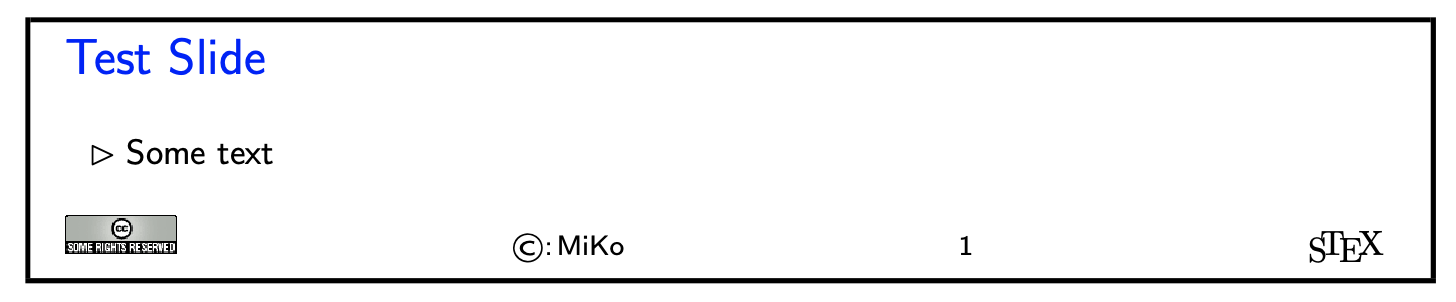
\includegraphics[width=.95\textwidth]{\stexdocpath/../lib/img/notes-frame}
  
The footer line can be customized. In particular the logos. 

\begin{function} {\setslidelogo}
  The default logo provided by the \pkg{notesslides} package is the {\sTeX} logo it can be
  customized using |\setslidelogo{|\meta{logo name}|}|.
\end{function}

\begin{function}{\setsource}
  The default footer line of the \pkg{notesslides} package mentions copyright and
  licensing. In \pkg{notesslides} |\source| stores the author's name as the copyright
  holder. By default it is the author's name as defined in the |\author| macro in the
  preamble.  |\setsource{|\meta{name}|}| can change the writer's name.
\end{function}

\begin{function}{\setlicensing}
  For licensing, we use the Creative Commons Attribuition-ShareAlike license by default to
  strengthen the public domain. If package |hyperref| is loaded, then we can attach a
  hyperlink to the license logo. |\setlicensing[|\meta{url}|]{|\meta{logo name}|}| is used
  for customization, where \meta{url} is optional.
\end{function}
\end{sfragment}

\begin{sfragment}[id=sec:user:frameimages]{Frame Images}
 Sometimes, we want to integrate slides as images after all -- e.g. because we already
have a PowerPoint presentation, to which we want to add \sTeX notes.

\begin{function}{\frameimage,\mhframeimage}
  In this case we can use |\frameimage[|\meta{opt}|]{|\meta{path}|}|, where \meta{opt} are
  the options of |\includegraphics| from the \pkg{graphicx} package~\cite{CarRah:tpp99}
  and \meta{path} is the file path (extension can be left off like in
  |\includegraphics|). We have added the |label| key that allows to give a frame label
  that can be referenced like a regular |beamer| frame.

The |\mhframeimage| macro is a variant of |\frameimage| with repository support. Instead
of writing
\begin{stexcode}
\frameimage{\MathHub{fooMH/bar/source/baz/foobar}}
\end{stexcode}
  we can simply write (assuming that |\MathHub| is defined as above)
\begin{stexcode}
\mhframeimage[fooMH/bar]{baz/foobar}
\end{stexcode}
  Note that the |\mhframeimage| form is more semantic, which allows more advanced document
management features in \textsf{MathHub}.
\end{function}

If |baz/foobar| is the ``current module'', i.e. if we are on the \textsf{MathHub} path
\ldots|MathHub/fooMH/bar|\ldots, then stating the repository in the first optional
argument is redundant, so we can just use
\begin{stexcode}
\mhframeimage{baz/foobar}
\end{stexcode}
\end{sfragment}

\begin{function}{\textwarning}
  The |\textwarning| macro generates a warning sign: \textwarning
\end{function}


\begin{sfragment}{Ending Documents Prematurely}
  \begin{function}{\prematurestop,\afterprematurestop}
    For prematurely stopping the formatting of a document, \sTeX provides the
    |\prematurestop| macro. It can be used everywhere in a document and ignores all input
    after that -- backing out of the |sfragment| environments as needed. After that -- and
    before the implicit |\end{document}| it calls the internal |\afterprematurestop|, which
    can be customized to do additional cleanup or e.g. print the bibliography.
  
    |\prematurestop| is useful when one has a driver file, e.g. for a course taught multiple
    years and wants to generate course notes up to the current point in the lecture. Instead
    of commenting out the remaining parts, one can just move the |\prematurestop| macro.
    This is especially useful, if we need the rest of the file for processing, e.g. to
    generate a theory graph of the whole course with the already-covered parts marked up as
    an overview over the progress; see |import_graph.py| from the |lmhtools|
    utilities~\cite{lmhtools:github:on}.
  \end{function}
  
  Text fragments and modules can be made more re-usable by the use of global variables. For
  instance, the admin section of a course can be made course-independent (and therefore
  re-usable) by using variables (actually token registers) |courseAcronym| and |courseTitle|
  instead of the text itself. The variables can then be set in the \sTeX preamble of the
  course notes file.
\end{sfragment}


\begin{sfragment}{Global Document Variables}
  To make document fragments more reusable, we sometimes want to make the content depend
  on the context. We use \defemph{document variables} for that.

\begin{function}{\setSGvar,\useSGvar}
  |\setSGvar{|\meta{vname}|}{|\meta{text}|}| to set the global variable \meta{vname} to
  \meta{text} and |\useSGvar{|\meta{vname}|}| to reference it.
\end{function}
  
\begin{function}{\ifSGvar}
  With|\ifSGvar| we can test for the contents of a global variable: the macro call
  |\ifSGvar{|\meta{vname}|}{|\meta{val}|}{|\meta{ctext}|}| tests the content of the global
  variable \meta{vname}, only if (after expansion) it is equal to \meta{val}, the
  conditional text \meta{ctext} is formatted.
\end{function}
\end{sfragment}

\begin{sfragment}[id=sec:user:excursions]{Excursions}
In course notes, we sometimes want to point to an ``excursion'' -- material that is either
presupposed or tangential to the course at the moment -- e.g. in an appendix. The typical
setup is the following:

\begin{stexcode}
\excursion{founif}{../fragments/founif.en}
  {We will cover first-order unification in}
...
\begin{appendix}\printexcursions\end{appendix}
\end{stexcode}

It generates a paragraph that references the excursion whose source is in the file
|../fragments/founif.en.tex| and automatically books the file for the |\printexcursions|
command that is used here to put it into the appendix. We will look at the mechanics now. 

\begin{function}{\excursion}
  The |\excursion{|\meta{ref}|}{|\meta{path}|}{|\meta{text}|}| is syntactic sugar for

\begin{stexcode}
\begin{nparagraph}[title=Excursion]
  \activateexcursion{founif}{../ex/founif}
  We will cover first-order unification in \sref{founif}.
\end{nparagraph}
\end{stexcode}
\end{function}

\begin{function}{\activateexcursion,\printexcursion,\excursionref}
  Here |\activateexcursion{|\meta{path}|}| augments the |\printexcursions| macro by a call
  |\inputref{|\meta{path}|}|. In this way, the |\printexcursions| macro (usually in the
  appendix) will collect up all excursions that are specified in the main text.

  Sometimes, we want to reference -- in an excursion -- part of another. We can use
  |\excursionref{|\meta{label}|}| for that.
\end{function}

\begin{function}{\excursiongroup}
  Finally, we usually want to put the excursions into an |sfragment| environment and add
  an introduction, therefore we provide the a variant of the |\printexcursions| macro:
  |\excursiongroup[id=|\meta{id}|,intro=|\meta{path}|]| is equivalent to
\begin{stexcode}
\begin{note}
\begin{sfragment}[id=<id>]{Excursions}
  \inputref{<path>}
  \printexcursions
\end{sfragment}
\end{note}
\end{stexcode}
\end{function}
\end{sfragment}

\begin{dangerbox}
  When option |book| which uses |\pagestyle{headings}| is given and semantic macros are
  given in the |sfragment| titles, then they sometimes are not defined by the time the
  heading is formatted. Need to look into how the headings are made. This is a problem of
  the underlying \pkg{document-structure} package.
\end{dangerbox}

%%% Local Variables:
%%% mode: latex
%%% TeX-master: "../stex-manual"
%%% End:

  \end{sfragment}
  \begin{sfragment}{Representing Problems and Solutions}
    \begin{sfragment}[id=sec:intro]{Introduction}

The |problem| package supplies an infrastructure that allows specify problem.  Problems
are text fragments that come with auxiliary functions: hints, notes, and
solutions\footnote{for the moment multiple choice problems are not supported, but may
  well be in a future version}. Furthermore, we can specify how long the solution to a
given problem is estimated to take and how many points will be awarded for a perfect
solution.

Finally, the |problem| package facilitates the management of problems in small files,
so that problems can be re-used in multiple environment. 

\begin{sfragment}{Package Options}
  \begin{function}{solutions,notes,hints,gnotes,pts,min,boxed,test}
    The |problem| package takes the options |solutions| (should solutions be output?),
    |notes| (should the problem notes be presented?), |hints| (do we give the hints?),
    |gnotes| (do we show grading notes?), |pts| (do we display the points awarded for
    solving the problem?), |min| (do we display the estimated minutes for problem
    soling). If theses are specified, then the corresponding auxiliary parts of the
    problems are output, otherwise, they remain invisible.

    The |boxed| option specifies that problems should be formatted in framed boxes so that
    they are more visible in the text. Finally, the |test| option signifies that we are in
    a test situation, so this option does not show the solutions (of course), but leaves
    space for the students to solve them.
  \end{function}
\end{sfragment}

\begin{sfragment}[id=sec:user:probsols]{Problems and Solutions}


\begin{environment}{problem}
  The main environment provided by the |problem| package is (surprise surprise) the
  |problem| environment. It is used to mark up problems and exercises. The environment
  takes an optional KeyVal argument with the keys |id| as an identifier that can be
  reference later, |pts| for the points to be gained from this exercise in homework or
  quiz situations, |min| for the estimated minutes needed to solve the problem, and
  finally |title| for an informative title of the problem.
\end{environment}

\begin{latexcode}
\usepackage[solutions,hints,pts,min]{problem}
\begin{document}
  \begin{sproblem}[id=elefants,pts=10,min=2,title=Fitting Elefants,name=elefants]
    How many Elefants can you fit into a Volkswagen beetle?
\begin{hint}
  Think positively, this is simple!
\end{hint}
\begin{exnote}
  Justify your answer
\end{exnote}
\begin{solution}[for=elefants,height=3cm]
  Four, two in the front seats, and two in the back.
\begin{gnote}
  if they do not give the justification deduct 5 pts
\end{gnote}
\end{solution}
  \end{sproblem}
\end{document}
\end{latexcode}

The result of formatting this problem is
\begin{minipage}{.9\linewidth}
\begin{sproblem}[id=elefants.prob,title=Fitting Elefants,name=elefants2]
  How many Elefants can you fit into a Volkswagen beetle?
\begin{hint}
  Think positively, this is simple!
\end{hint}
\begin{exnote}
  Justify your answer
\end{exnote}
\smallskip\noindent\hrule\textbf{Solution:}
  Four, two in the front seats, and two in the back.
\hrule
\end{sproblem}
\end{minipage}

\begin{environment}{solution}
  The |solution| environment can be to specify a solution to a problem. If the package
  option |solutions| is set or |\solutionstrue| is set in the text, then the solution will
  be presented in the output. The |solution| environment takes an optional KeyVal argument
  with the keys |id| for an identifier that can be reference |for| to specify which
  problem this is a solution for, and |height| that allows to specify the amount of space
  to be left in test situations (i.e. if the |test| option is set in the |\usepackage|
  statement).
\end{environment}

\begin{environment}{hint,exnote,gnote}
  The |hint| and |exnote| environments can be used in a |problem| environment to give
  hints and to make notes that elaborate certain aspects of the problem.  The |gnote|
  (grading notes) environment can be used to document situtations that may arise in
  grading.
\end{environment}

\begin{function}{\startsolutions,\stopsolutions}
  Sometimes we would like to locally override the |solutions| option we have given to the
  package. To turn on solutions we use the |\startsolutions|, to turn them off,
  |\stopsolutions|. These two can be used at any point in the documents.
\end{function}

\begin{function}{\ifsolutions}
  Also, sometimes, we want content (e.g. in an exam with master solutions) conditional on
  whether solutions are shown. This can be done with the |\ifsolutions| conditional.
\end{function}
\end{sfragment}

\begin{sfragment}[id=sec:user:mcq]{Multiple Choice Blocks}

\begin{environment}{mcb}
  Multiple choice blocks can be formatted using the |mcb| environment, in which single
  choices are marked up with |\mcc| macro.
\end{environment}

\begin{function}{\mcc}
  |\mcc[|\meta{keyvals}|]{|\meta{text}|}| takes an optional key/value argument
  \meta{keyvals} for choice metadata and a required argument \meta{text} for the proposed
  answer text. The following keys are supported
  \begin{itemize}
  \item |T| for true answers, |F| for false ones,
  \item |Ttext| the verdict for true answers, |Ftext| for false ones, and
  \item |feedback| for a short feedback text given to the student.
  \end{itemize}
\end{function}

\begin{latexcode}
\begin{sproblem}[title=Functions,name=functions1]
  What is the keyword to introduce a function definition in python?
  \begin{mcb}
    \mcc[T]{def}
    \mcc[F,feedback=that is for C and C++]{function}
    \mcc[F,feedback=that is for Standard ML]{fun}
    \mcc[F,Ftext=Nooooooooo,feedback=that is for Java]{public static void}
  \end{mcb}
\end{sproblem}
\end{latexcode}
This results in 

\begin{sproblem}[title=Functions,name=functions2]
  What is the keyword to introduce a function definition in python?
  \begin{mcb}
    \mcc[T]{def}
    \mcc[F,feedback=that is for C and C++]{function}
    \mcc[F,feedback=that is for Standard ML]{fun}
    \mcc[F,Ftext=Nooooooooo,feedback=that is for Java]{public static void}
  \end{mcb}
\end{sproblem}
\solutionstrue\hrule
\begin{sproblem}[title=Functions,name=functions3]
  What is the keyword to introduce a function definition in python?
  \begin{mcb}
    \mcc[T]{def}
    \mcc[F,feedback=that is for C and C++]{function}
    \mcc[F,feedback=that is for Standard ML]{fun}
    \mcc[F,Ftext=Nooooooooo,feedback=that is for Java]{public static void}
  \end{mcb}
\end{sproblem}
\end{sfragment}

\begin{sfragment}[id=sec:user:includeproblem]{Including Problems}
  
\begin{function}{\includeproblem}
  The |\includeproblem| macro can be used to include a problem from another file. It takes
  an optional KeyVal argument and a second argument which is a path to the file containing
  the problem (the macro assumes that there is only one problem in the include file). The
  keys |title|, |min|, and |pts| specify the problem title, the estimated minutes for
  solving the problem and the points to be gained, and their values (if given) overwrite
  the ones specified in the |problem| environment in the included file.
\end{function}
\end{sfragment}

\begin{sfragment}[id=sec:user:reporting]{Reporting Metadata}
The sum of the points and estimated minutes (that we specified in the |pts| and |min|
keys to the |problem| environment or the |\includeproblem| macro) to the log file and
the screen after each run. This is useful in preparing exams, where we want to make sure
that the students can indeed solve the problems in an allotted time period.

The |\min| and |\pts| macros allow to specify (i.e. to print to the margin) the
distribution of time and reward to parts of a problem, if the |pts| and |pts| package
options are set. This allows to give students hints about the estimated time and the
points to be awarded.
\end{sfragment}

\begin{sfragment}[id=sec:limitations]{Limitations}

In this section we document known limitations. If you want to help alleviate them,
please feel free to contact the package author. Some of them are currently discussed in
the \sTeX GitHub repository~\cite{sTeX:github:on}. 
\begin{enumerate}
\item none reported yet
\end{enumerate}
\end{sfragment}
\end{sfragment}

%%% Local Variables:
%%% mode: latex
%%% TeX-master: "../stex-manual"
%%% End:

  \end{sfragment}
  \begin{sfragment}{Homeworks, Quizzes and Exams}
  
The \pkg{wexam} package and class supplies an infrastructure that allows to format
nice-looking assignment sheets by simply including problems from problem files marked up
with the \pkg{roblem} package.  It is designed to be compatible with |problems.sty|, and
inherits some of the functionality.

\begin{sfragment}[id=sec:user:options]{Package Options}

\begin{variable}{solutions,notes,hints,gnotes,pts,min}
  The \pkg{wexam} package and class take the options |solutions|, |notes|, |hints|,
  |gnotes|, |pts|, |min|, and |boxed| that are just passed on to the \pkg{problems}
  package (cf. its documentation for a description of the intended behavior).
\end{variable}
\end{sfragment}

\begin{sfragment}{Assignments}
This package supplies the \DescribeEnv{assignment}|assignment| environment that groups
problems into assignment sheets. It takes an optional KeyVal argument with the keys
\DescribeMacro{number}|number| (for the assignment number; if none is given, 1 is
assumed as the default or --- in multi-assignment documents --- the ordinal of the
|assignment| environment), \DescribeMacro{title}|title| (for the assignment title; this
is referenced in the title of the assignment sheet), \DescribeMacro{type}|type| (for the
assignment type; e.g. ``quiz'', or ``homework''), \DescribeMacro{given}|given| (for the
date the assignment was given), and \DescribeMacro{due}|due| (for the date the
assignment is due).
\end{sfragment}

\begin{sfragment}{Typesetting Exams}

Furthermore, the \pkg{hwexam} package takes the option
\DescribeMacro{multiple}|multiple| that allows to combine multiple assignment sheets
into a compound document (the assignment sheets are treated as section, there is a table
of contents, etc.).

Finally, there is the option \DescribeMacro{test}|test| that modifies the behavior to
facilitate formatting tests. Only in |test| mode, the macros |\testspace|,
|\testnewpage|, and |\testemptypage| have an effect: they generate space for the
students to solve the given problems. Thus they can be left in the {\LaTeX} source. 

\DescribeMacro{\testspace}|\testspace| takes an argument that expands to a dimension,
and leaves vertical space accordingly. \DescribeMacro{\testnewpage}|\testnewpage| makes
a new page in |test| mode, and \DescribeMacro{\testemptypage}|\testemptypage| generates
an empty page with the cautionary message that this page was intentionally left empty.

Finally, the \DescribeEnv{testheading}|\testheading| takes an optional keyword argument
where the keys \DescribeMacro{duration}|duration| specifies a string that specifies the
duration of the test, \DescribeMacro{min}|min| specifies the equivalent in number of
minutes, and \DescribeMacro{reqpts}|reqpts| the points that are required for a perfect
grade.

\begin{latexcode}
\title{320101 General Computer Science (Fall 2010)}
\begin{testheading}[duration=one hour,min=60,reqpts=27]
  Good luck to all students!
\end{testheading}
\end{latexcode}

Will result in
\begin{center}
  \begin{minipage}{.9\textwidth}
\makeatletter
\@problem{1.1}{4}{10}
\@problem{2.1}{4}{8}
\@problem{2.2}{6}{10}
\@problem{2.3}{6}{10}
\@problem{3.1}{4}{8}
\@problem{3.2}{4}{8}
\@problem{3.3}{2}{4}
\makeatother
\vspace*{-3ex}\hrule\vspace*{.5ex}  formats to\vspace*{1ex}
\hrule\par\noindent\vspace*{2ex}
\title{320101 General Computer Science (Fall 2010)}
\begin{testheading}[duration=one hour,min=60,reqpts=27]
  good luck
\end{testheading}
\end{minipage}
\end{center}
\end{sfragment}

\begin{sfragment}{Including Assignments}

The \DescribeMacro{\inputassignment}|\inputassignment| macro can be used to input
an assignment from another file. It takes an optional KeyVal argument and a second
argument which is a path to the file containing the problem (the macro assumes that
there is only one |assignment| environment in the included file).  The keys
\DescribeMacro{number}|number|, \DescribeMacro{title}|title|,
\DescribeMacro{type}|type|, \DescribeMacro{given}|given|, and \DescribeMacro{due}|due|
are just as for the |assignment| environment and (if given) overwrite the ones specified
in the |assignment| environment in the included file.
\end{sfragment}

%%% Local Variables:
%%% mode: latex
%%% TeX-master: "../stex-manual"
%%% End:

  \end{sfragment}
\end{sfragment}

\csname if@infulldoc\endcsname\else
\newpage 
\printbibliography
\end{document}
\fi

%%% Local Variables:
%%% mode: latex
%%% TeX-master: t
%%% End:

%  LocalWords:  stex-docheader infulldoctrue l@subsubsection toclevel@part ExplSyntaxOff
%  LocalWords:  l_document_structure_section_level_int dangerbox mmtbox omdoc OBJref lmh
%  LocalWords:  own:fifom MueRabRot:rslffml20 sec.stexarchives stex-mathhub ngerman a,b
%  LocalWords:  Metatheory sec.customhighlight sproof stexthm xspace stexpatchmodule
%  LocalWords:  stexpatchexample stexpatchparagraph sexampleid amsthm sassertiontitle
%  LocalWords:  sdefinitiontitle compemph varemph srefsymuri stex-hwexam TeXLive:on tlmgr
%  LocalWords:  stexls:on,stexls-vscode-plugin:on
